\documentclass[a4paper,fleqn]{cas-dc}

% If the frontmatter runs over more than one page
% use the longmktitle option.

%\documentclass[a4paper,fleqn,longmktitle]{cas-dc}

\usepackage{color,colortbl}
\definecolor{ligthYellow}{RGB}{255,255,204}
\definecolor{ligthBlue}{RGB}{193,255,255}
\definecolor{ligthRed}{RGB}{255,231,231}
\definecolor{ligthViolet}{RGB}{235,235,255}
\definecolor{ligthGreen}{RGB}{204,255,204}

\usepackage{makecell}

\usepackage[numbers]{natbib}
%\usepackage[authoryear]{natbib}
%\usepackage[authoryear,longnamesfirst]{natbib}

%%%Author macros
\def\tsc#1{\csdef{#1}{\textsc{\lowercase{#1}}\xspace}}
\tsc{WGM}
\tsc{QE}
%%%

% Uncomment and use as if needed
%\newtheorem{theorem}{Theorem}
%\newtheorem{lemma}[theorem]{Lemma}
%\newdefinition{rmk}{Remark}
%\newproof{pf}{Proof}
%\newproof{pot}{Proof of Theorem \ref{thm}}

\begin{document}
\let\WriteBookmarks\relax
\def\floatpagepagefraction{1}
\def\textpagefraction{.001}

% Short title
\shorttitle{Meta--heuristic parameter estimation of solar cells with S--shaped IV characteristics}

% Short author
\shortauthors{O. Olikh}

% Main title of the paper
\title [mode = title]{Estimation of parameters for solar cells with S--shaped current--voltage characteristics using meta--heuristic algorithms}

% First author
%
% Options: Use if required
% eg: \author[1,3]{Author Name}[type=editor,
%       style=chinese,
%       auid=000,
%       bioid=1,
%       prefix=Sir,
%       orcid=0000-0000-0000-0000,
%       facebook=<facebook id>,
%       twitter=<twitter id>,
%       linkedin=<linkedin id>,
%       gplus=<gplus id>]
\author{Oleg~Olikh}
%\cormark[1]
\ead{olegolikh@knu.ua}
%\address[1]{Taras Shevchenko National University of Kyiv, 64/13, Volodymyrska Street, City of Kyiv, Ukraine, 01601}


% Address/affiliation
\affiliation{organization={Taras Shevchenko National University of Kyiv},
            addressline={64/13, Volodymyrska Street},
            city={Kyiv},
%          citysep={}, % Uncomment if no comma needed between city and postcode
            postcode={01601},
 %           state={},
            country={Ukraine}}

% For a title note without a number/mark
%\nonumnote{}

% Here goes the abstract
\begin{abstract}
Defect-assisted recombination processes frequently
limit the photovoltaic device performance.
The low-cost and express methods of impurity contamination control
are in demand at solar cell manufacturing.
In this paper, we applied deep learning-based
approach to extract the iron concentration in silicon solar cell from an
ideality factor values.
\end{abstract}

% Use if graphical abstract is present
%\begin{graphicalabstract}
%\includegraphics{}
%\end{graphicalabstract}

% Research highlights
\begin{highlights}
\item Proposed deep learning-based method to predict iron contamination in Si-SC by using IV curve.
\item The simulated IV characteristics are used to create training and test datasets.
\item The DNN's configurations are proposed.
\item The mean squared relative error of prediction is up to 0.005.
\end{highlights}

% Keywords
% Each keyword is seperated by \sep
\begin{keywords}
S--shaped current--voltage characteristics \sep Opposed two-diode model \sep Parameter estimation \sep
Meta--heuristic algorithms \sep Nonparametric statistical procedure \sep Solar cell models
\end{keywords}

\maketitle

% Main text
\section{Introduction}\label{Int}

Photovoltaics (PV) is widely regarded as the most promising sustainable
clean energy technology to meet the rising energy demand of our global population.
By the end of 2021, the installed capacity of global solar PV panels reached an impressive 971 GW,
with an additional 183 GW added in 2021 alone \cite{Divya2023}.
According to the International Energy Agency (IEA) reports, the cumulative installed PV capacity
was predicted to increase to 1.826 TW by 2026 and 14.5 TW by 2050 \cite{Wang2022}.
Currently, silicon solar cells make up approximately 90\% of the global photovoltaic production capacity.
But recently, intensive research is underway for innovative developments,
further experiments, and practical PV applications of various new-generation solar cells (SCs).
The operating principle of new-generation solar cells is qualitatively similar to silicon-based ones.
However, it is important to note that the fourth quadrant of their current-voltage (IV) characteristics
often exhibits an S-shaped deformation or kink.
This kink’s origin has been attributed to various physical phenomena:
charge trapping at the cathode interface \cite{Sesa2019,Finck2013},
rectifying Schottky junction at the anode interface \cite{Zuo2014}
change of the electric field distribution \cite{Castro2010},
presence of strong interface dipoles \cite{Romero2017},
unbalanced charge transport \cite{Gao2011}.
Furthermore, it is worth noting that such a feature of the IV characteristics is typical
in the most promising candidates for the next generation of photovoltaic devices.
Specifically, S-shaped IV curves have been observed in silicon heterojunction SCs \cite{Saive2019},
thin-film SCs such as CdTe, CI(G)S, and amorphous silicon PV devices \cite{Saive2019,Roland2016},
normal and inverted organic SCs \cite{Gaur2014,Tran2017,Lastra2019},
perovskite SCs \cite{Saive2019,Xu2016},
quantum dot SCs \cite{Gao2011,Yu2019a},
and hybrid SCs \cite{VeinbergVidal2016,Romero2017,Finck2013}.


One of the most common approaches to understanding the electrical characteristics of PV devices
is to use an equivalent circuit model to fit the shape of the IV curve.
Such lumped-parameter modeling allows simulation, analysis, and optimization of device performance.
The most frequently used conventional solar cell lumped-parameter models are single-diode model (SDM), double-diode
model (DDM), and three-diode model (TDM) models.
The models incorporate parallel-connected diodes that activate in one direction,
a photo-current source, a parallel shunt resistance, and a series resistance.
The PV module model (PVMM) is based on SDM and is made up of several diodes in series or parallel.

Unfortunately, the conventional models failed in describing the S-shaped kink.
Thus, new models are proposed to give some reasonable IV curve shape explanations on the IV curve shape from the view of electricity.
One of the earliest attempts to develop such a model was proposed by Mazhari \cite{Mazhari2006}.
This model is essentially a simplified version of the SDM, achieved by excluding resistances and incorporating an additional diode.
Up to now, Mazhari’s model is the simplest circuit because the least fitting parameters are required for simulations.
Mazhari’s model fails to capture the linear-like rise S-shaped kink in the third quadrant,
and the model, which improved by incorporating two resistance, proposed for organic SCs \cite{Yu2019}.
Gaur and Kumar \cite{Gaur2014} proposed equivalent circuit models to represent the behavior of polymer solar in the dark.
This model is almost identical to the DDM, except one of the diodes is the opposite.
Another way to develop equivalent models involved using multiple series diodes, unlike conventional approaches.
Zuo \emph{et al}. \cite{Zuo2014} offered to explain the S-shape by utilizing a model consisting
of two series diodes connected in the same direction, two shunt resistors, and one series resistor.
Another lumped-parameter equivalent circuit holds two opposed diodes, two opposed current sources, and no resistors \cite{Gao2011}.
De Castro et al \cite{Castro2010} proposed a model consisting of two opposed diodes with shunt resistance for each,
a series resistance, and a photo-current source.
The last model represents a significant advancement
as it successfully reproduces the S-shaped kink in the power-producing fourth quadrant
of the illuminated IV characteristics.
However, it falls short of adequately describing the IV curve
beyond the open-circuit point in the first quadrant,
where the current of many practical devices tends to continue increasing \cite{SshapeRewShot}.
To address this challenge, a potential solution was suggested ---
incorporating a third diode that would either replace one of the shunt resistances \cite{GarciaSanchez2013}
or be placed in parallel with it \cite{DeCastro2016,Roland2016}.
In general, the developing models to describe S-shaped IV curves continues.
For instance, a relatively recent proposal \cite{Sesa2019} is the B2BDM model:
back-to-back diodes in parallel with a shunt resistor and the photo-current source, all in series with an offset voltage source, and
then connected in parallel to another diode and shunt resistor, again in series with a resistor.
Some review about models for PV devices with S-shaped IV curves can be found in \cite{SshapeRewShot,GarciaSanchez2017}.

The next step after developing the model is to identify the corresponding parameters from the IV characteristics. 
Essentially, this task is an optimization problem.
One popular approach for solving such problems is the application of meta--heuristic algorithms. 
In fact, there have been numerous meta--heuristic algorithms developed specifically for this purpose.
The No Free Lunch theory (NFL) \cite{NFL} provides the foundation for such diversity, 
stating that no single meta--heuristic algorithm can solve all optimization tasks effectively.
In other words, the optimization algorithm can have brilliant results in a specific class of problems 
and at the same time fails to solve other ones.
As a result, each problem, including the parameter estimation of each equivalent model, necessitates a distinct algorithm selection.
Numerous studies have been conducted to compare the efficiency of meta-heuristic algorithms for parameter estimation under conventional SC models. 
Some studies focus on a single model, such as SDM \cite{DE_EM}, DDM \cite{SSA,FWA}, or TDM \cite{ELSHADE_INR}, 
while others examine both SDM and DDM concurrently \cite{BBO_M,CSO,BPFPA,MPALW}.
Several papers have investigated algorithms' efficiency in processing IV curves according to three models: SDM, DDM, and PVMM \cite{IMPA,SCA_NM_OBL,MPSO,IWOA,IJAYA}.
Indeed, the utilization of conventional SC models for testing newly developed 
algorithms is among the most popular approaches after using CEC20XX test functions.
The wide range of metaheuristic optimization methods allows for situations in which 
various studies examine identical models but prioritize different algorithms array.


%Що ж до оцінки параметрів відповідно до  models for PV devices with S-shaped IV curves, то тут ситуація не настільки ж райдужна.
%Звичайно, метаеврістичні алгоритми застосовуються до обробки екпериментальних S-подібних ВАХ [], проте роботи, присвячені вибору найбільш ефективного підходу до вирішення подібної задачі нам нажаль невідомі. Хоча, відповідно до NFL theory, не можна очікувати, що алгоритми, які показали чудові результати для моделей кремнієвих монокристалічних сонячних елементів, будуть настільки ж ефективні у і випадку моделей для next generation of photovoltaic devices with S-shaped IV curves.
%
%Метою даного дослідження було порівняння ефективності визначення параметрів відповідно до дво-діодної моделі Кастро для набору з 14 метаеврістичних алгоритмів та визначення кращого з них.
%Вибір саме цієї моделі з усього різноманіття зумовлений тим що вона є достатньо універсальною.
%Незважаючи на вказані вище її недоліки у першому квадранті, вона привертає увагу з точки зору
%знаходження аналітичних рівнянь, які описують ВАХ,
%deriving the analytical solutions of the equivalent circuits
%а також широко
%використовується для опису експериментально отриманих ВАХ сонячних елементів з різною будовою.
%Зокрема мова йде про polymer та polymer/fullerene bulk heterojunction photocell, ternary organic solar cells \cite{Makha2018} та інші типи органічних структур,
%perovskite SC with fullerene transport layer and the carbon nanotube  electrode,  and perovskite SC with ionic liquid gating та багато інших.
%Розглянуті метаеврістичні алгоритми належать до різних категорій відносно their sources of inspiration, деякі з них є достатньо класичними, інші - більш новітніми, розробленими з врахуванням досвіду використання попередників.
%Отримані результати порівнюються з використанням різноманітних методів непараметричної статистики.
%
%
%This study aimed to determine the best
%algorithms
%
% conventional solar cell
%
%In the literature, meta-heuristics are frequently categorized based on their sources of inspiration.


%------------------------------------
%organic \cite{Pillai2017} GA
%organic \cite{Arredondo2018}


%perovskite SC with fullerene electron transport layer and the carbon nanotube  top electrode \cite{CastroUsePerovskitIonikLiquid}
%Ionic Liquid Gating in Perovskite Solar Cells with Fullerene/Carbon Nanotube Collectors \cite{CastroUsePerovskitFullerene}
%\cite{CastroUseBook}
%
%organic solar cells through gold ion implantation in the PEDOT:PSS laye \cite{BrenesBadilla2018}
%---------------------------------------------
%An S-shaped current–voltage characteristic is frequently observed in a photovoltaic
%cell using emerging materials such as organic semiconductors and organic–
%inorganic perovskite materials. \cite{Tada2021}
%
%small molecular bulk heterojunction photocells
%using a composite consisting of p-DTS(FBTTh2)2 and neat
%C70 (organic) \cite{Tada2015Organic}
%
% photocell \cite{Tada2017}
%
%ternary organic solar cells \cite{Makha2018}
%
%polymer/fullerene  organic \cite{delPozo2012}
% typical phenomenon in BHJ
%solar cells is the appearance of a ‘‘kink’’ or S-shape in the J–V
%characteristic.
%This bulk
%heterojunction (BHJ)
%

%-----------------------------------------------------
%\cite{Yu2019a}
%
%
%In fact, the most important attribution of our manuscript is
%deriving the analytical solutions of the reported circuits [7,14,17] to
%improve the simulation efficiency and giving the detailed discussions
%about the effects from the model parameters on
%
%-------------------------------------





%\section{Models and Methods}\label{MM}
\section{Problem definition}\label{MM}
\subsection{Solar cell model}\label{SCModel}
Fig.~\ref{fig_chem}
vividly reveals the structure of the used model \cite{Castro2010}.
It can be seen from the figure that model contains a current source accompanied by a diode D1, a shunt
resistor $R_\mathrm{p1}$ to show the leakage current, and a series resistor $R_\mathrm{s}$ to consider the
losses associated with the load current.
Besides, the second diode D2 with a second parallel resistance $R_\mathrm{p2}$ is placed opposite to the first one and is essential to
simulate the non-ideal effects of the active layer/cathode interface.
In this model, D1 is responsible for the exponential behavior of the IV curve,
the main contribution of D2 is to simulate the S--shape.
The analytical solution $V(I)$ of the opposed two--diode equivalent circuit model was
 obtained \cite{CastroSolution} using Lambert $W$-function \cite{LambertNew}:


\begin{figure}[]
	\centering
		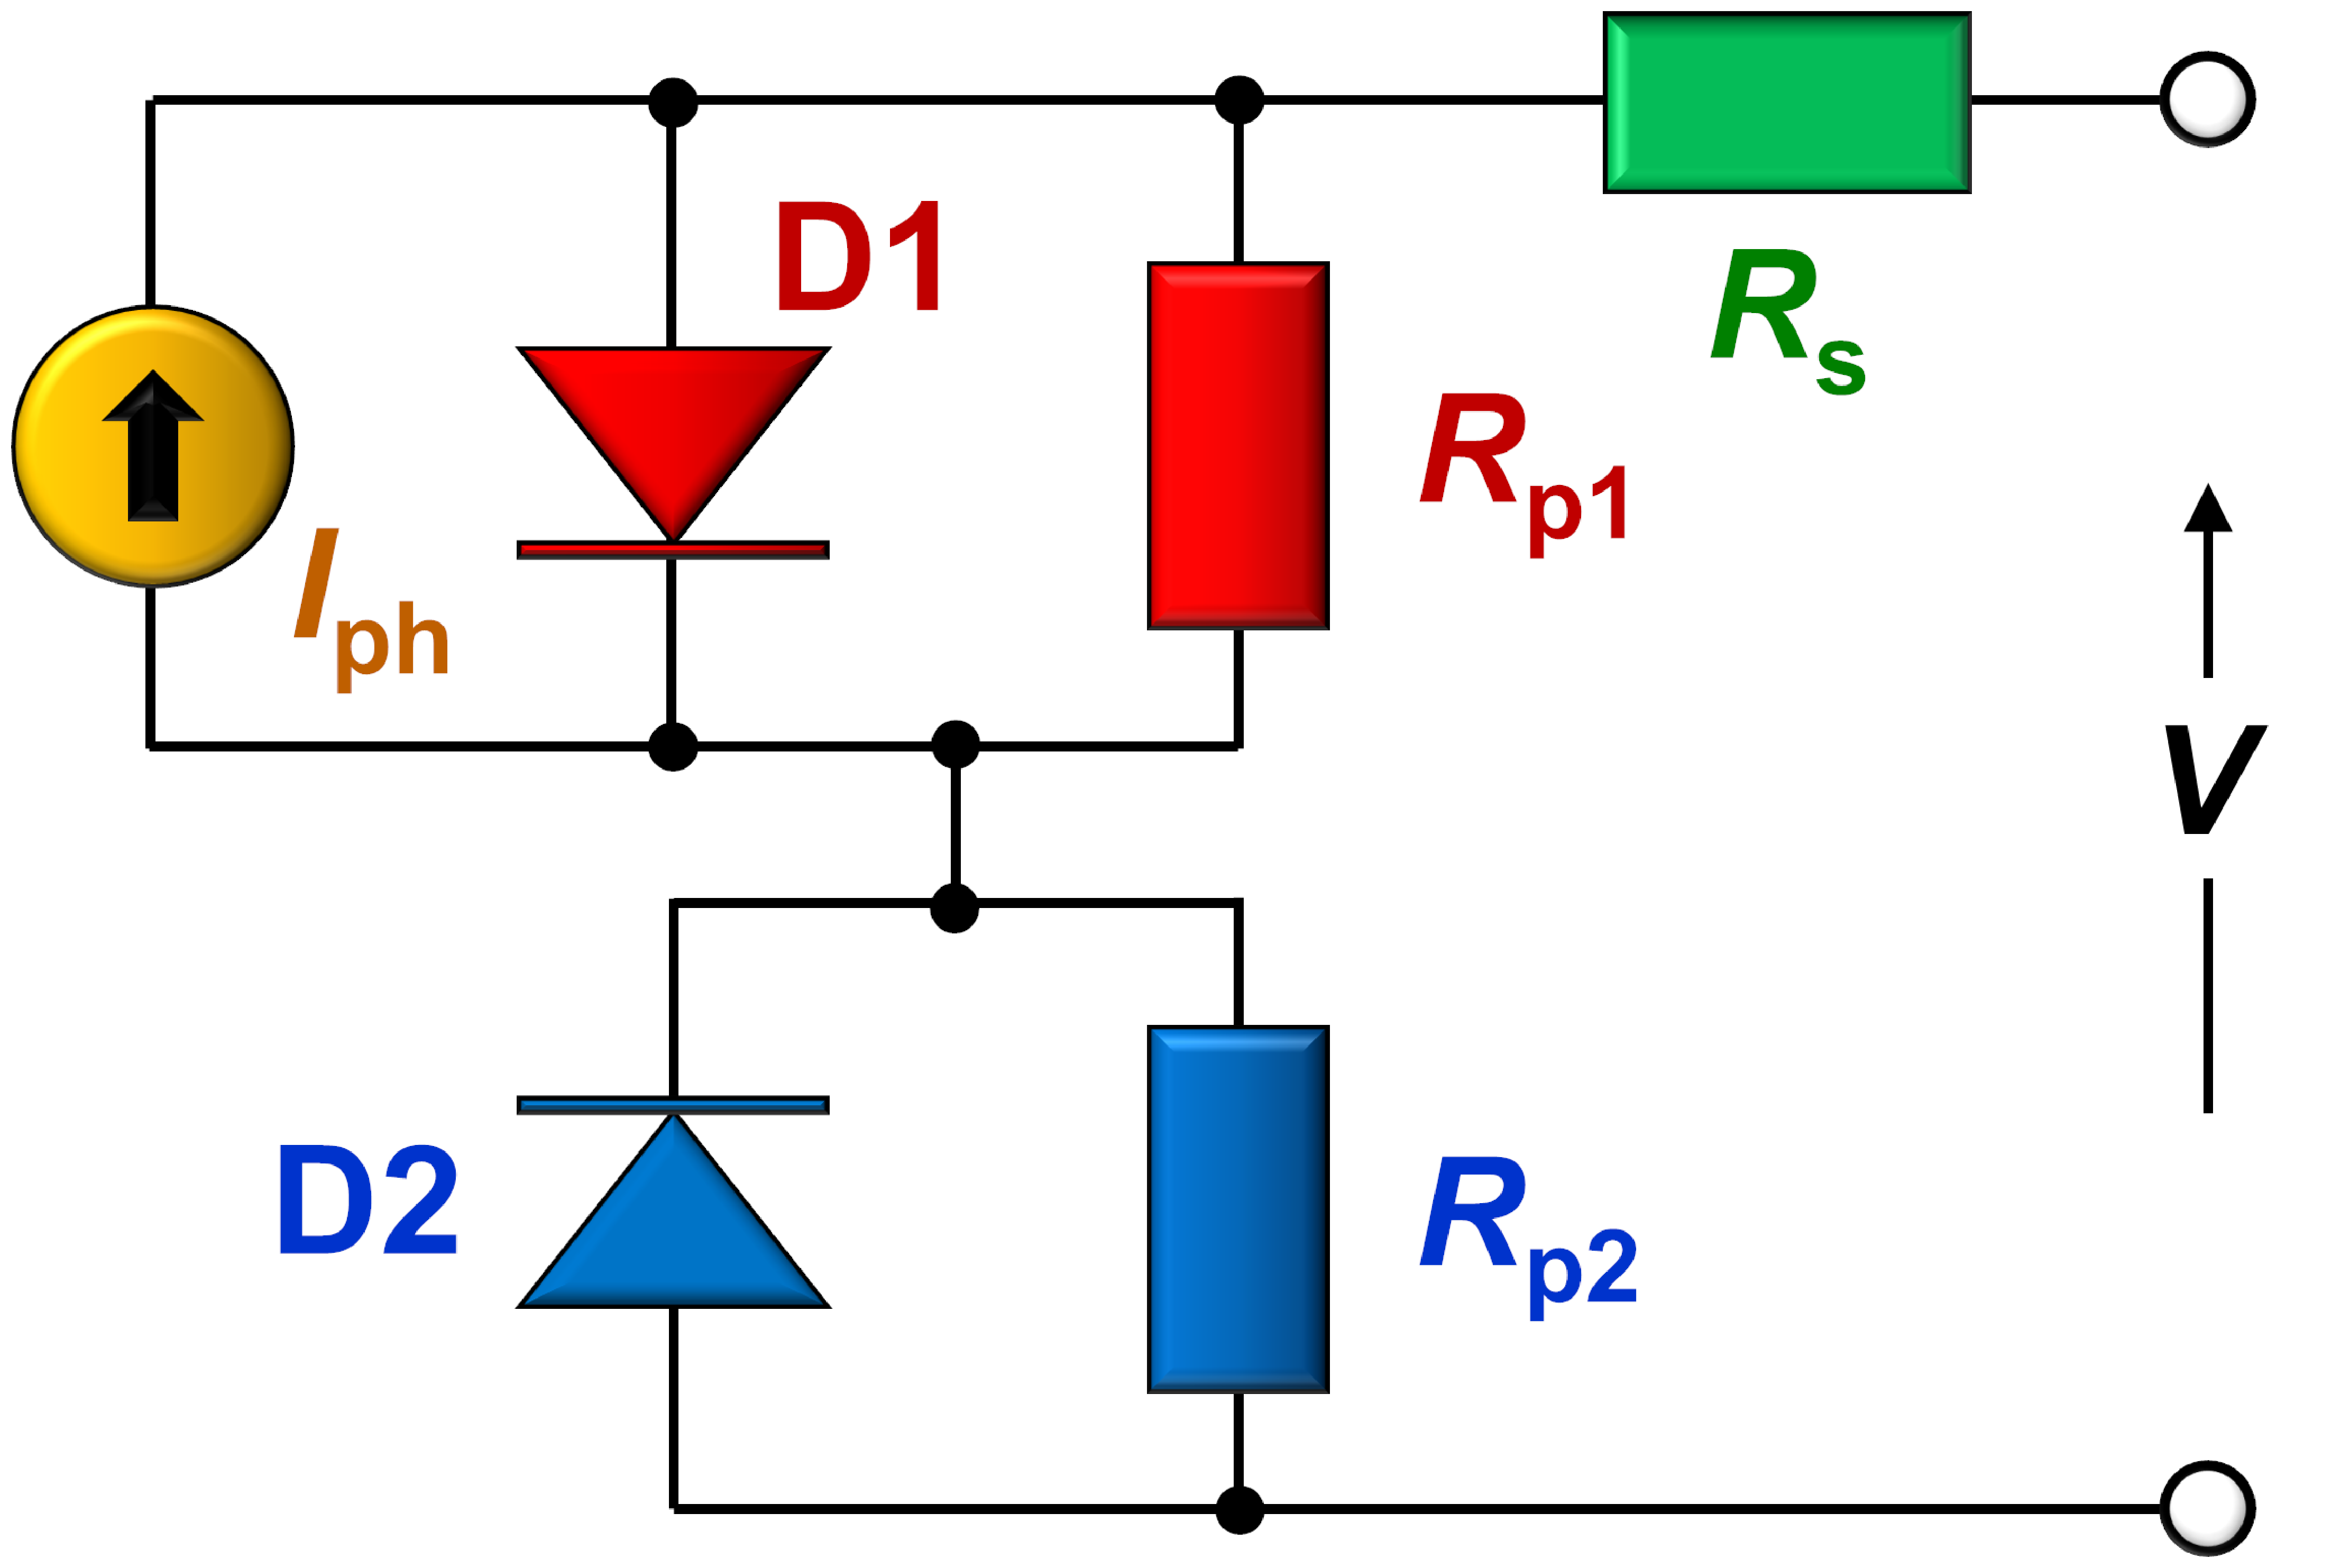
\includegraphics[width=0.9\columnwidth]{Chem}
	  \caption{The opposed two--diode equivalent--circuit model of a solar cell.}\label{fig_chem}
\end{figure}


\begin{eqnarray}
% \nonumber to remove numbering (before each equation)
\label{eqIV_W}
V&=& (I+I_\mathrm{ph}+I_{01})R_\mathrm{p1} \nonumber \\
  &&-\frac{n_1kT}{q}W\left\{\frac{qI_{01}R_\mathrm{p1}}{n_1kT}\exp\left[\frac{qR_\mathrm{p1}(I+I_\mathrm{ph}+I_{01})}{n_1kT}\right]\right\} \nonumber \\
  &&+\frac{n_2kT}{q}W\left\{\frac{qI_{02}R_\mathrm{p2}}{n_2kT}\exp\left[-\frac{qR_\mathrm{p2}(I-I_{02})}{n_2kT}\right]\right\} \nonumber \\
  &&+(I-I_{02})R_\mathrm{p2}+IR_\mathrm{s}\,,
\end{eqnarray}
where
$I_{01}$ and $I_{02}$ are the saturation currents and
$n_1$ and $n_2$ are
the ideality factors for D1 and D2 respectively,
and $I_\mathrm{ph}$ is the ideal photocurrent.
Thus, the model employs eight lumped parameters
($I_{01}$, $n_1$, $R_\mathrm{p1}$, $I_{02}$, $n_2$, $R_\mathrm{p2}$,
$R_\mathrm{s}$, and $I_\mathrm{ph}$)
that need to be determined from the IV curve.
Thus, from an optimization perspective, the dimension of the problem is $D=8$.

The expression~(\ref{eqIV_W}) has a drawback in that it tends to stray from the range of numbers that can be accommodated by the standard 64-bit floating-point format owing to the presence of exponential functions for larger numbers.
To overcome this drawback, the use of the $g$--function $g(x)=\ln(W(\exp(x)))$ was suggested \cite{roberts2015calculating}.
The analytical solution $V(I)$ using the $g$--function is as follows \cite{roberts2015calculating}
\begin{equation}
\label{eqIV_g}
\begin{split}
V(I)= &IR_\mathrm{s}+\frac{n_1kT}{q}g(x_1)-\frac{n_2kT}{q}g(x_2) \\
  &-\frac{n_1kT}{q}\ln\left[\frac{qI_{01}R_\mathrm{p1}}{n_1kT}\right] +\frac{n_2kT}{q}\ln\left[\frac{qI_{02}R_\mathrm{p2}}{n_2kT}\right]\,,
\end{split}
\end{equation}
with
\begin{equation}
\label{eqx1}
x_1= \ln\left(\frac{qI_{01}R_\mathrm{p1}}{n_1kT}\right)+\frac{q(I+I_\mathrm{ph}+I_{01})R_\mathrm{p1}}{n_1kT}\,,
\end{equation}
and
\begin{equation}
\label{eqx2}
x_2= \ln\left(\frac{qI_{02}R_\mathrm{p2}}{n_2kT}\right)-\frac{q(I-I_{02})R_\mathrm{p2}}{n_2kT}\,.
\end{equation}
We used Eqs.~(\ref{eqIV_g})--(\ref{eqx2}) both for simulation IV curves and during the approximation procedure.
The $g$--function was evaluated by using iterative procedure \cite{roberts2015calculating}.

\subsection{Synthetic IV curves}\label{SynIV}
The research involved the parameter estimation of solar cells using meta-heuristic algorithms based
on synthetic IV characteristics simulated using the opposed two--diode model.
This approach allows for assessing the accuracy of the employed optimization methods,
as the simulation was performed using known parameter values.

In first part of the study, a detailed analysis was conducted on a single IV curve,
evaluating the performance of meta--heuristic algorithms for parameter estimation in a one--time application mainly.
Additionally, the suitability of employing two different fitness functions was examined.
In the second part, we simulated a set of IV characteristics and evaluated the average performance metrics of various algorithms.

\subsubsection{Single--IV case}\label{SingleIV}

Previous studies have demonstrated \cite{Tada2015Organic,Tada2021} that when the ideality factor of D2 is either equal to or significantly larger than $n_1$
($n_1=n_2=1.92$ or $n_1=1.00$, $n_2=3.00$), the nonlinear least--squares method successfully determines a set of equivalent circuit parameters
that accurately replicate the experimental data of an organic photovoltaic cell.
Therefore this approach does not allow for distinguishing between similar IV curves obtained from solar cells with different parameters.
To overcome this issue, Tada \cite{Tada2021} successfully employed Bayesian estimation of parameters.
To assess the capabilities of meta-heuristic methods in overcoming additional similar challenges,
they were applied to a IV curve corresponding to such a problematic case.
The parameter values were taken from \cite{Tada2021}:
\begin{equation}
\label{eqParSingleIV}
\begin{split}
I_{01}&=1.6\cdot10^{-6}\,\text{mA},\\
n_1&=1.92,\\
R_\mathrm{p1}&=190\,\Omega,\\
I_{02}&=0.16\,\text{mA},\\
n_2&=1.92,\\
R_\mathrm{p2}&=190\,\Omega,\\
R_\mathrm{s}&=45\,\Omega,\\
I_\mathrm{ph}&=8\,\text{mA},
\end{split}
\end{equation}
%($I_{01}=1.6\cdot10^{-6}$~mA,
%$n_1=1.92$,
%$R_\mathrm{p1}=190$~$\Omega$,
%$I_{02}=0.16$~mA,
%$n_2=1.92$,
%$R_\mathrm{p2}=190$~$\Omega$,
%$R_\mathrm{s}=45$~$\Omega$,
%$I_\mathrm{ph}=8$~mA),
and the IV curve was simulated over a range of 0-0.8~V with step 10~mV at $T=300$~K.
The simulation result is presented on Fig.~\ref{figSigleIV} by symbols.


\begin{figure}[]
	\centering
		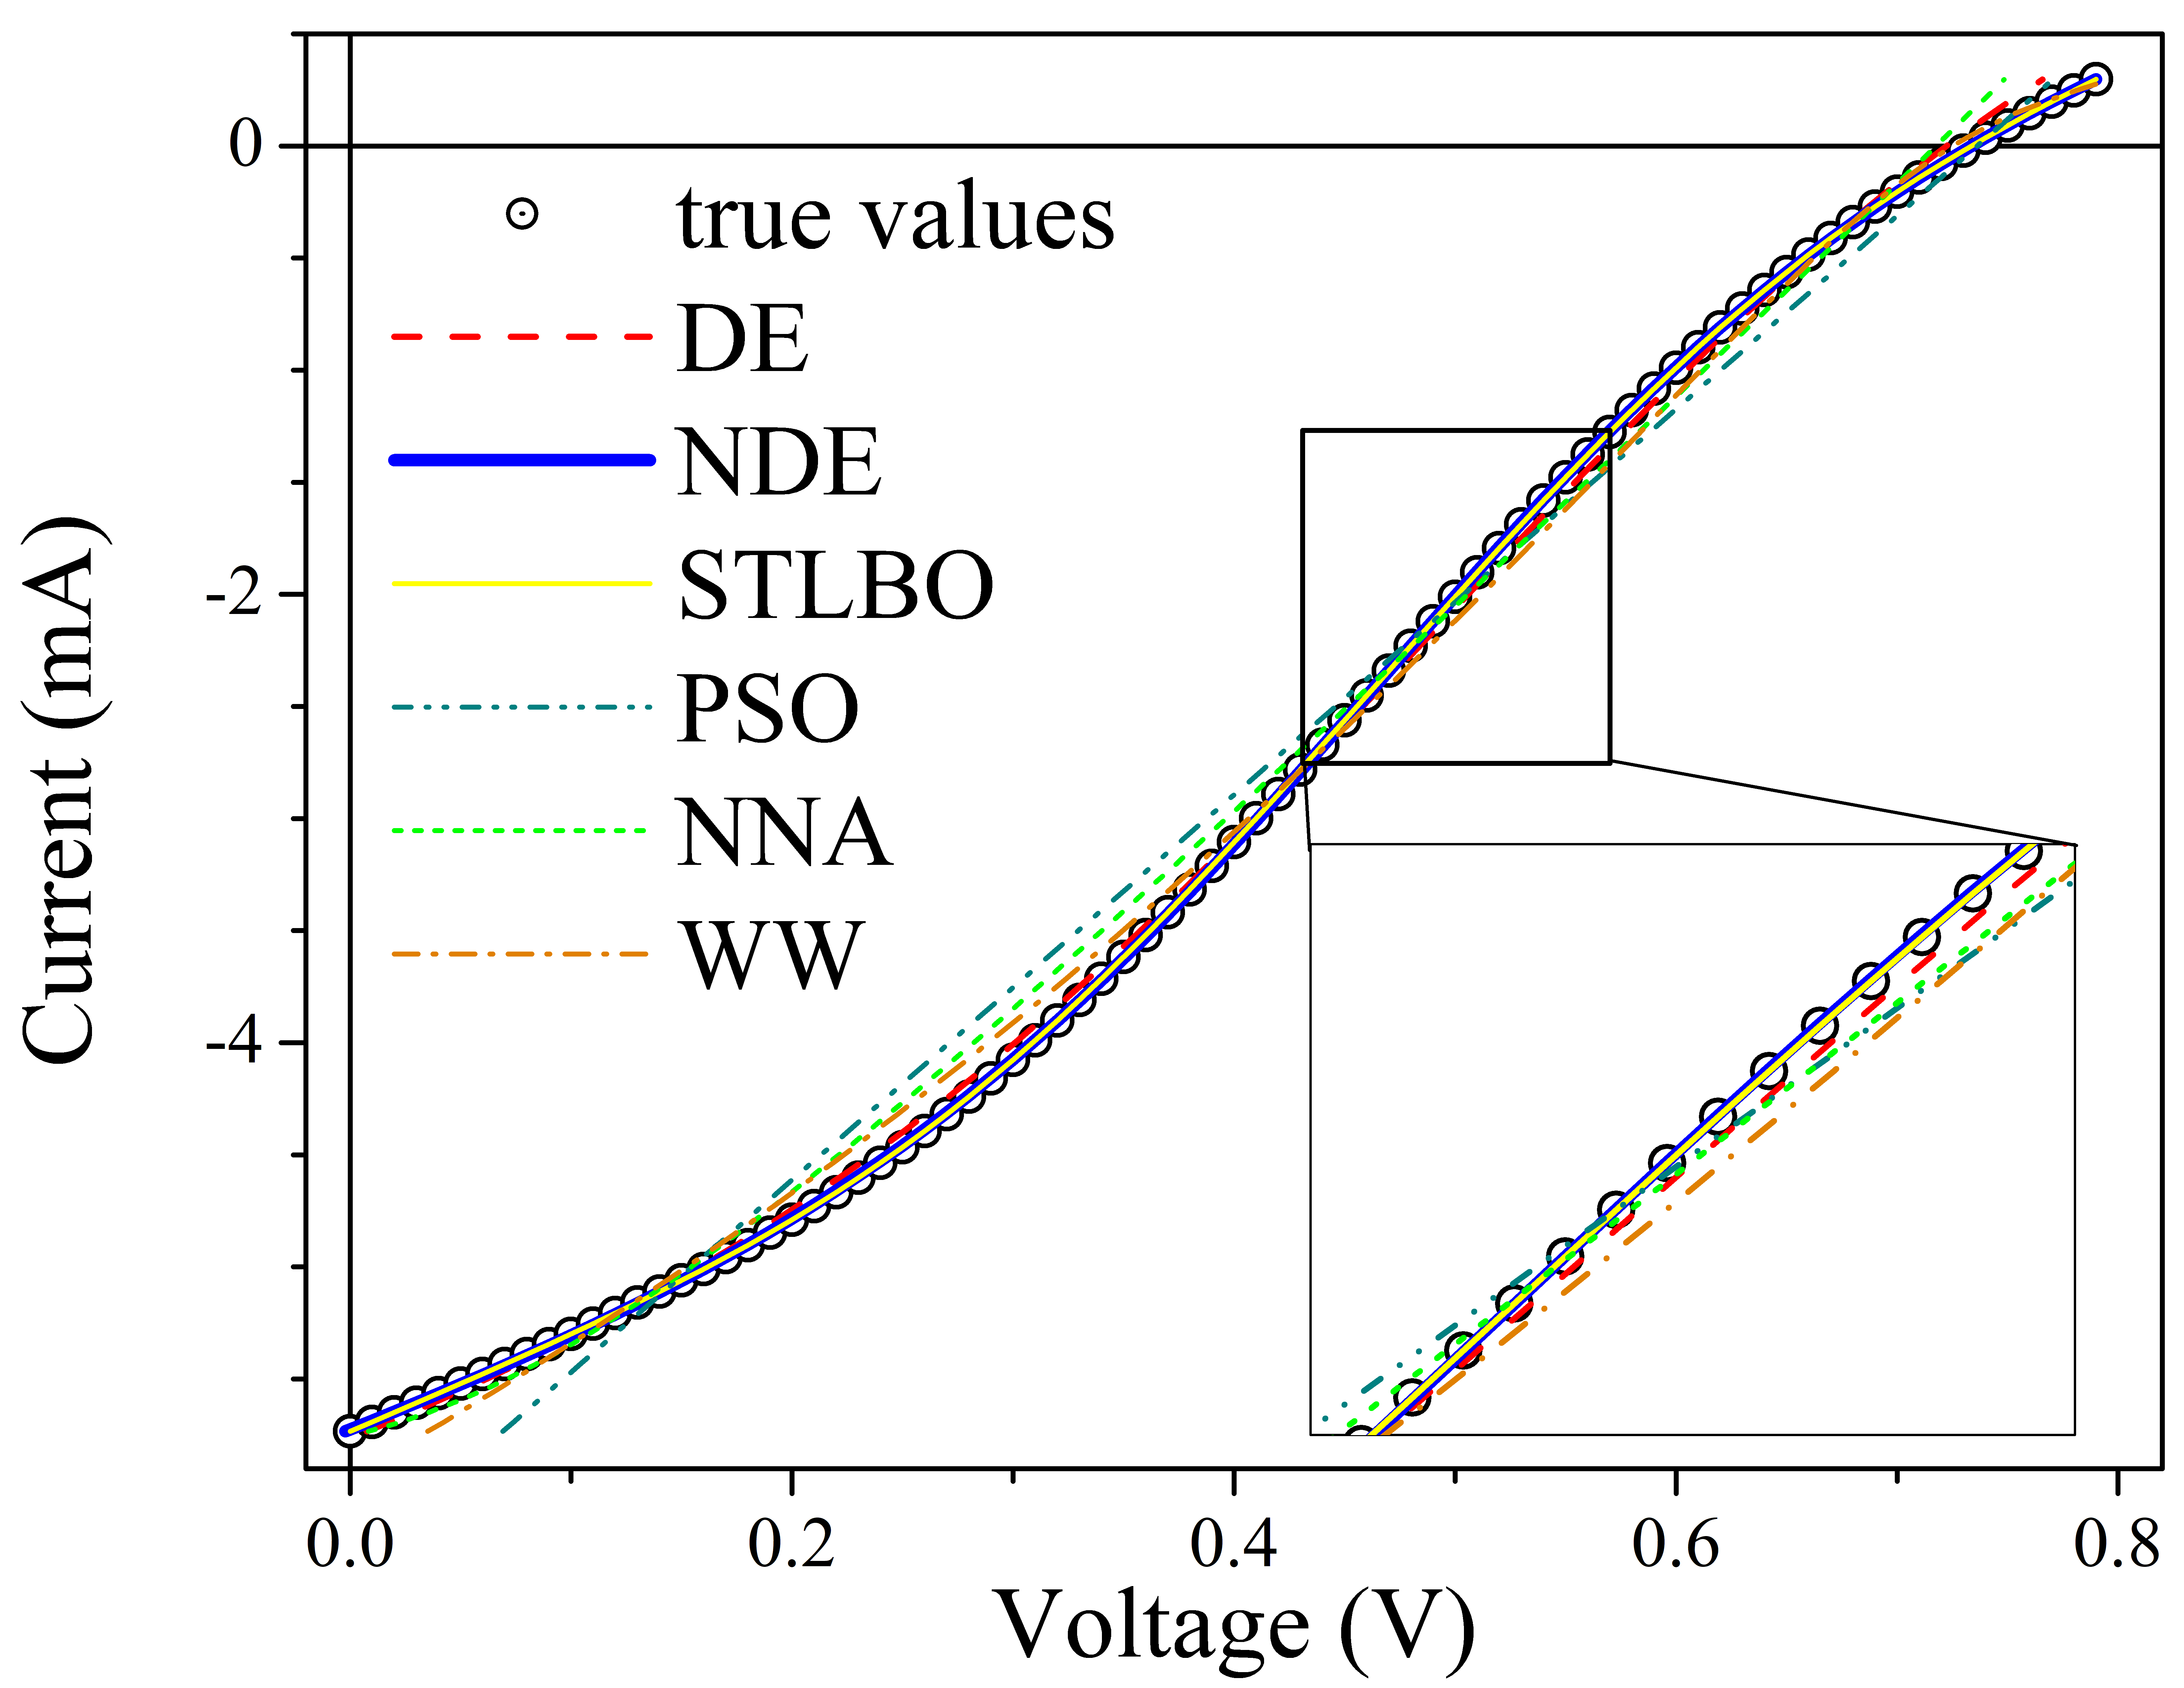
\includegraphics[width=1.0\columnwidth]{IVsimple}
	  \caption{Fitting results (lines) for the simulated current-voltage characteristic (symbols).
             The values from  Eq.~(\ref{eqParSingleIV}) were assumed under simulation.}\label{figSigleIV}
\end{figure}

%It has been shown previously whether the ideality factor of D2 ($n_2$) is the same as that of D1
%($n_1=n_2=1.92$) or very larger than $n_1$ ($n_1=1.00$, $n_2=3.00$),
%the nonlinear least--squares method finds a set of equivalent circuit parameters that reproduces the experimental
%data of an organic photovoltaic cell.


\subsubsection{IV--set case}\label{SetIV}
Employing various meta--heuristic algorithms to analyze a single IV curve
is insufficient to obtain comprehensive insights into the methods' efficacy in parameter estimation.
The accuracy of parameter determination is closely tied to their absolute values.
For instance, an increase in the $R_\mathrm{p}$ value can pose challenges for accurately estimating resistance
because the shunt will have a lesser impact on the overall shape of IV curve.
In addition, the ratio between the parameter values also plays a crucial role.

To test the methods across different parameter values, we generated synthetic data in a temperature range from 260 K to 350 K.
During the simulation process, we considered various temperature dependencies of the parameters.
We based our approach on known physical mechanisms but focused on achieving the diversity of parameter ratio
instead of attempting to replicate real--life photovoltaic converters precisely.
Furthermore, an S--shaped IV curve is observed in solar cells of various types,
and diverse charge transport mechanisms significantly complicate the selection of
the only possible temperature dependence for each of the eight model parameters.
Therefore, we assumed that the current conduction mechanism through D1 is close to tunneling,
and hence, $I_{01}$, $R_\mathrm{p1}$, and $(n_1kT)$ remain constant,
with $I_{01}=0.015$~mA, $R_\mathrm{p1}=10^4$~$\Omega$, $n_1kT=7$~eV.
In the case of D2, the thermionic emission current was suggested
and $I_{02}$ and $n_2$ increased and decreased, respectively, with temperature rise \cite{Sze2012}:
\begin{eqnarray}
%\label{eqIV_W}
I_{02}&=& I_{002}\exp\left(-\frac{E_I}{kT}\right)\,,\\
n_2&=&1+\frac{T^*}{T}\,,
\end{eqnarray}
where $I_{002}$, $E_I$, and $T^*$ are the constants which are independent of temperature.
The values of $I_{002}=500$~A, $E_I=0.40$~eV, and $T^*=500$~K were used.
For $R_\mathrm{p2}$, an exponential temperature dependence was employed,
as it is widely observed \cite{Kondratenko2019} in modern solar cells for the shunt resistance:
\begin{equation}
R_\mathrm{p2}=R_\mathrm{p20}\exp\left(\frac{E_R}{kT}\right)\,.
\end{equation}
with
$R_\mathrm{p20}=9$~m$\Omega$,
$E_R=0.32$~eV.
The linear temperature dependencies is expected for both $I_\mathrm{ph}$ \cite{Green2003,Eberle2021} and $R_\mathrm{s}$ \cite{Ibrahim2017,Bradaschia2019}:
\begin{equation}
y=y_{0}[1+\mathrm{TC}_y(T-300)]\,,
\end{equation}
where
$y=I_\mathrm{ph}$ or $R_\mathrm{s}$,
$y_0$ is the parameter value at room temperature,
$\mathrm{TC}_y$ is the temperature coefficient of parameter.
For most types of monocrystalline silicon solar cells, the $\mathrm{TC}_{I_\mathrm{ph}}$ typically ranges from around $-0.0004$~K$^{-1}$ \cite{TuanLe2021}.
However, as the base thickness decreases, the temperature coefficient can increase to $-0.0014$~K$^{-1}$ \cite{Dupre2016}.
For hydrogenated amorphous silicon solar cells, $\mathrm{TC}_{I_\mathrm{ph}}$ is equal to $-10^{-3}$~K$^{-1}$ \cite{Riesen2016}.
For organic solar cells, the temperature coefficient can reach a magnitude of $-0.003$~K$^{-1}$ \cite{Rana2018}.
During the simulation, we assumed $\mathrm{TC}_{I_\mathrm{ph}}=-10^{-3}$~K$^{-1}$.
Furthermore, the values of $I_\mathrm{ph0}=1$~mA,
$\mathrm{TC}_{R_\mathrm{s}}=0.02$~K$^{-1}$,
and $R_\mathrm{s0}=50$~$\Omega$ were used.



%Thus, the set of synthetic IV curves was generated using the following temperature dependencies of the parameters:
%\begin{equation}
%\label{eqParSetIV}
%\begin{split}
%I_{01}(T)[\text{mA}]&=0.015\,,\\
%n_1(T)&=(7kT)^{-1},\\
%R_\mathrm{p1}(T)[\Omega]&=10^4\,,\\
%I_{02}(T)[\text{mA}]&=10^3\exp\left(-\frac{0.40}{kT}\right)\,,\\
%n_2&=1.92,\\
%R_\mathrm{p2}&=190\,\Omega,\\
%R_\mathrm{s}&=45\,\Omega,\\
%I_\mathrm{ph}&=8\,\text{mA},
%\end{split}
%\end{equation}
The set of I–V data was composed of 10 curves,
which were simulated at 10~K intervals from 260 to 350~K;
in this case,
$n_1$,
$I_{02}$,
$n_2$,
$R_\mathrm{p2}$,
$R_\mathrm{s}$,
and $I_\mathrm{ph}$
varied
from 6.37 to 4.73,
from 9 to 880 $\mu$A,
from 2.92 to 2.43,
from $1.4\cdot10^4$ to 360~$\Omega$,
from 10 to 100~$\Omega$,
and from 0.96 to 1.05~mA, respectively.
The simulation results are presented on Fig.~\ref{figSetIV} by symbols.
\begin{figure}[]
	\centering
		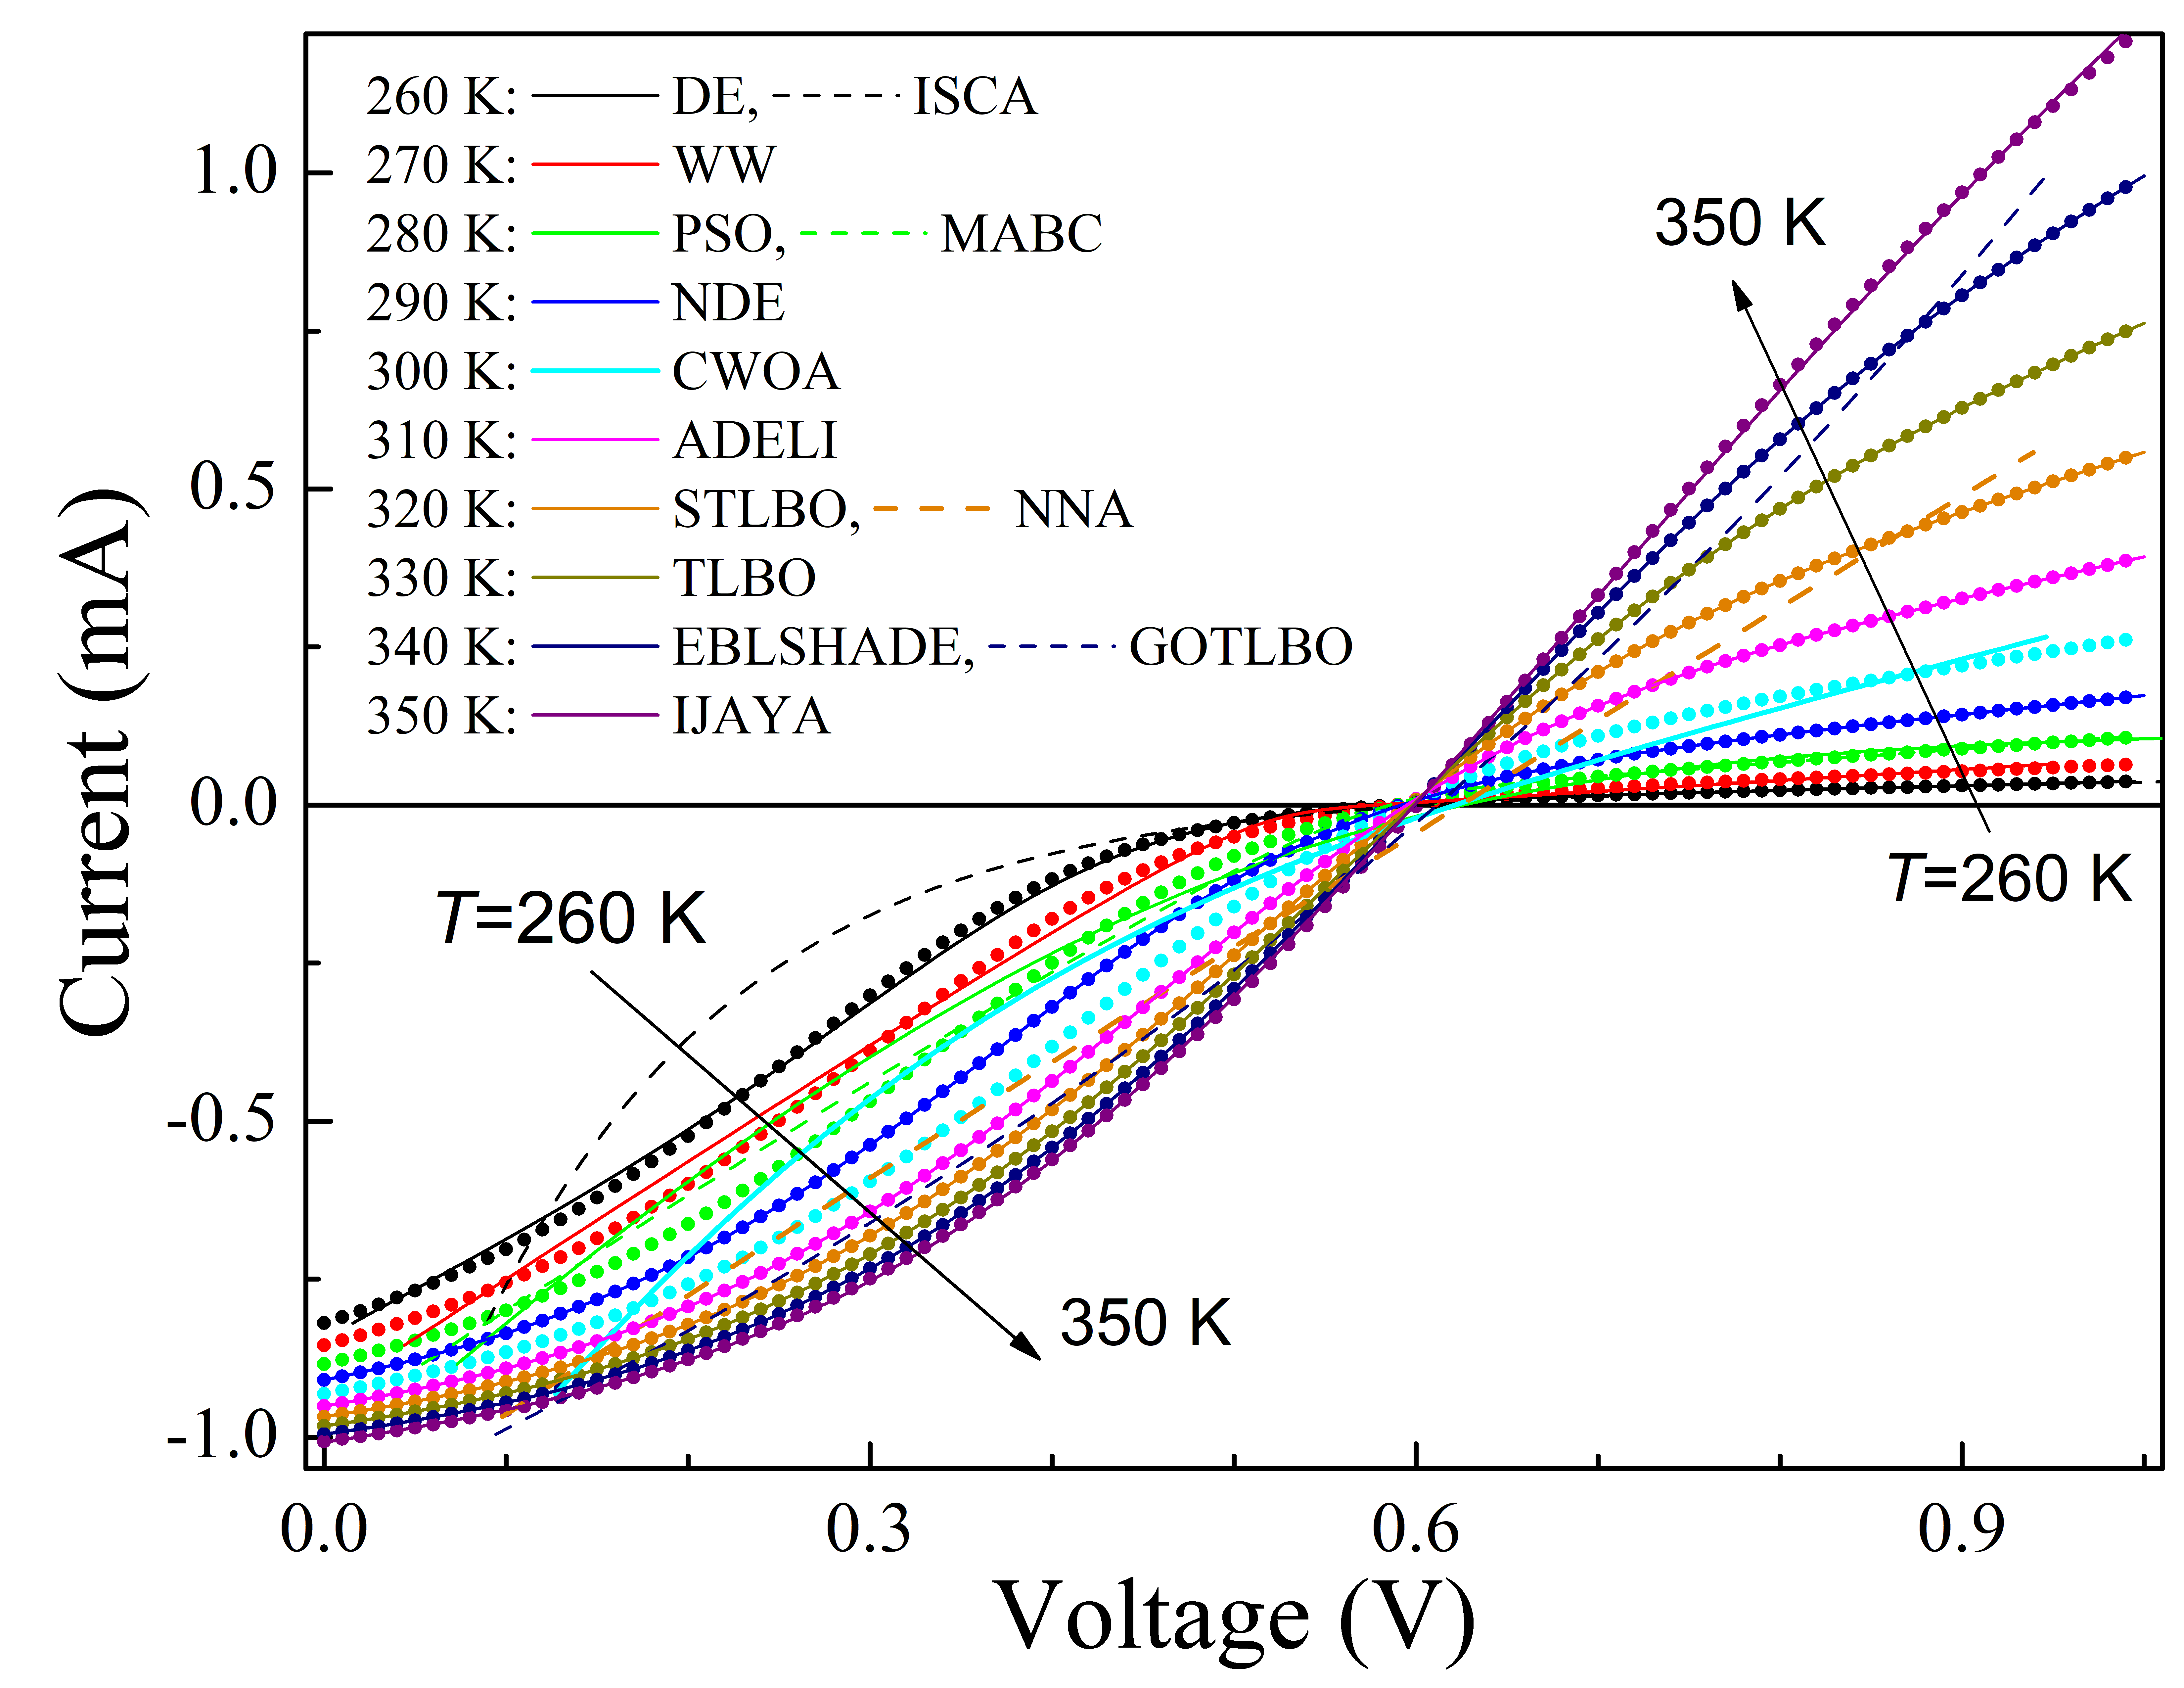
\includegraphics[width=1.0\columnwidth]{IVset}
	  \caption{Fitting results (lines) for the simulated current-voltage characteristic (symbols).
             The values from  Sec.~\ref{SetIV} were assumed under simulation.}\label{figSetIV}
\end{figure}

%перекласти на англійську "Таким чином, узагальнюючи, при створенні набору штучних ВАХ були використані наступні температурні залежності параметрів"



%виправити стилістичні помилки ""

%Estimation of parameters for solar cells with S--shaped current--voltage characteristics using meta--heuristic algorithms

\subsection{Meta-heuristic algorithms}\label{MHA}
In the literature, meta-heuristics are frequently categorized based on their sources of inspiration.
This categorization involves incorporating elements of true simulations and principles that incorporate stochasticity,
with the objective of emulating diverse characteristics observed in biological behavior, the lives of creatures in nature, human behavior, or natural phenomena.
On this basis, any meta-heuristic algorithm can fall into one of the following main classes \cite{WhiteShark,Gannet,Dandelion}:
evolution-based methods (emulate the principles of evolutionary behavior observed in creatures in nature by relying on the concept of survival of the fittest),
swarm intelligence--based methods (simulate the collective, dynamic, intelligent, and concerted gregarious conduct of collections of flocks or communities found in nature),
bio--based methods (use biological processes unrelated to group behavior),
chemical \& physical--based methods (originate from the physical phenomena or chemical laws that exist in the universe),
human-society--based methods (inspired by human beings, including various activities such as thinking and social behavior),
and math--based methods (borrow the mathematical functions).
Generally, there are hundreds of meta-heuristic optimization methods available.
While we acknowledge that our selection may not be fully comprehensive,
we utilized 14 methods, representing all classes mentioned above,
to tackle the parameter estimation task within the framework of the opposed two-diode model for a solar cell.
Hereafter, we provide a succinct description of each method alongside the parameters employed during the fitting process.

\emph{Differential evolution} (\textbf{DE}).
DE is one of the classical methods,
and  it is based on the natural selection law and uses the randomly generated initial population,
differential mutation, and probability crossover \cite{DEWang}.
During the implementation, we employed a penalty function suggested by Ishaque \emph{et al} \cite{P-DE_Ishaque}.
Besides, according to Wang and Ye \cite{DEWang}, the values of mutation scaling factor $F=0.8$,
crossover rate $C\!r=0.3$, and population size $N\!p=8\times D=64$ were used in this work.

\emph{Adaptive differential evolution with the Lagrange interpolation argument} (\textbf{ADELI}).
The method is based on DE, which integrates an adaptive local search scheme with Lagrange interpolation \cite{ADELI}.
This incorporation aims to enhance the exploitation capability and accelerate the convergence speed.
In ADELI, the scaling factor and crossover rate are set to self--adapting to optimize the results.
We used parameter values recommended by Huang \emph{et al} \cite{ADELI} during the implementation process.
Additionally, we set $N\!p$ to 64 for our numerical experiments.

\emph{Differential evolution with neighborhood--based adaptive evolution mechanism} (\textbf{NDE}).
The method uses a mutation strategy, which takes into account neighborhood and individual information, and an adaptive evolution mechanism \cite{NDE}.
The determination of $F$ and $C\!r$ values is achieved through the utilization of the weighted adaptive procedure \cite{Tanabe2014},
and an adaptive adjustment of the population size is implemented using a simple reduction method (from $10\times D=80$ to 5).

\emph{Success history based DE with hybridization mutation strategies and population size reduction} (\textbf{EBLSHADE}).
The method is the hybridization framework between \emph{pbest} and \emph{ord\_pbest} mutation strategies
and stores a set of $Cr$ and $F$ values that have performed well in the recent past \cite{EBLSHADE}.
A linear $N\!p$ reduction (from $18\times D=144$ to 4) is used as well.

\emph{Particle swarm optimization} (\textbf{PSO}).
It is another classic method based on observations of the social behavior of animals,
such as bird flocking, fish schooling, and swarm theory.
According to Ye et al. \cite{PSO},  the values of learning factors $l_1=l_2=2$,
the final weight and the initial weight $w_{max}=0.9$, $w_{min}=0.4$, and
$N\!p=15\times D=120$ are used in this work.

The \emph{modified artificial bee colony} (\textbf{MABC}) algorithm is based
on the intelligent foraging behavior of honey bee swarms \cite{MABC}.
The control parameters include the population size ($N\!p=8\times D=64$)
and the maximum number of generations after which each non-improved food source is to be discarded ($L_{imit}=36$).

\emph{Chaotic Whale Optimization Algorithm} (\textbf{CWOA}).
WOA draws inspiration from the hunting behavior of humpback whales \cite{WOA}.
On the other hand, CWOA employs chaotic maps to compute and dynamically adjust its internal parameters \cite{CWOA}.
In our study, we utilized the Singer chaotic map and set $N\!p=100$ for the identification of the parameters of the solar cell.

The \emph{Neural Network Algorithm} (\textbf{NNA}) is a meta-heuristic algorithm that draws inspiration from
both biological nervous systems and artificial neural networks \cite{NNA}.
The recommended \cite{NNA} value $N\!p=50$ is used in our paper.

The \emph{teaching learning based optimization} (\textbf{TLBO}) algorithm employs the concept of passing on knowledge
within a classroom.
Similar to learners acquiring knowledge from a teacher and interacting with their peers,
TLBO incorporates such interactions \cite{TLBO_Patel}.
In this study, a value of $N\!p=100$ is utilized.

\emph{Generalized oppositional teaching learning based optimization} (\textbf{GOTLBO}).
This method integrates a concept that incorporates both the current estimate
and its opposite estimate simultaneously into the original TLBO algorithm
through the initialization step and generation jumping \cite{GOTLBO}.
The values of jumping rate $J\!r=1.0$ and $N\!p=20$ were used.

\emph{Simplified teaching-learning based optimization algorithm} (\textbf{STLBO}).
In STLBO, an elite strategy is employed to improve the searching capability,
and a the chaotic map is used to enrich the uniformity of random values in the mutation phase \cite{STLBO}.
The logistic chaotic map and $N\!p=20$ were used.


\emph{Water wave optimization} (\textbf{WWO}) takes inspiration from shallow water wave models
and borrows ideas from wave propagation, refraction, and breaking \cite{WW}.
WWO is easy to implement with a small-size population, and there are four control parameters:
the maximum wave height $h_{max}$,
the wavelength reduction coefficient $\alpha$,
the breaking coefficient $\beta$,
and the maximum number $k_{max}$ of breaking directions.
According to Zheng \cite{WW}, we used
the values $h_{max}=6$, $\alpha=1.026$,  $N\!p=10$,
$k_{max}=\min(12,D/2)=4$, and $\beta$ linearly decreased from 0.25 to 0.001.

\emph{Improved JAYA} (\textbf{IJAYA}).
Jaya algorithm is based on the concept
that the solution obtained for a given problem should move toward the best solution and should
avoid the worst solution and does not require any algorithm-specific parameter \cite{JAYA}.
In IJAYA, a self-adaptive weight is introduced to adjust the tendency of approaching the best solution
and avoiding the worst solution;
an experience-based learning strategy is employed to maintain the population diversity and enhance the exploration ability,
and a chaotic elite learning method is proposed to refine the quality of the best solution in each generation \cite{IJAYA}.
The logistic chaotic map and $N\!p=4\times D=32$ were used.

\emph{Improved sine cosine algorithm} (\textbf{ISCA}).
SCA based on simulating the behaviors of sine and cosine mathematical functions \cite{SCA}.
ISCA implementation included a modified position-updating equation based on inertia weight
($w_{start}=1$, $w_{end}=1$),
a nonlinear conversion parameter strategy based on the Gaussian function
($a_{start}=2$, $a_{end}=0$) \cite{ISCA2},
the creation of the opposite population to jump out from the local optima with $J\!r=0.1$ \cite{ISCA3},
a greedy selection, and $N\!p=30$.

The majority of the utilized algorithms demonstrate excellent performance when
it comes to parameter estimation of solar cells within conventional models (single or double diode) \cite{CWOA,DEWang,GOTLBO,IJAYA,MABC,PSO,STLBO,TLBO_Patel,LSHADE,IWOA}.

In meta-heuristic optimization methods, the quality of the extracted parameters is evaluated using the fitness function at
every iteration.
In our investigation, absolute error and square error fitness functions were under consideration:
\begin{equation}
\label{eqFae}
F_\mathrm{AE}(Y)= \sum_{k=1}^p \left|V^\mathrm{tr}(I_k)-V^\mathrm{cal}(I_k,Y)\right|\,,
\end{equation}
\begin{equation}
\label{eqFse}
F_\mathrm{SE}(Y)= \sum_{k=1}^p \left[V^\mathrm{tr}(I_k)-V^\mathrm{cal}(I_k,Y)\right]^2\,,
\end{equation}
where
$V^\mathrm{tr}(I_k)$ is the simulated value of voltage at current $I_k$,
$V^\mathrm{cal}(I_k,Y)$ is the calculated values of voltage, which can be obtained
by Eqs.~(\ref{eqIV_g})--(\ref{eqx2}),
for given set of parameters (i.e. $Y = \{I_{01},n_1,R_\mathrm{p1},I_{02},n_2,R_\mathrm{p2},R_\mathrm{s},I_\mathrm{ph}\}$)
at current $I_k$,
and $p$ is the total number of voltage steps in the IV characteristic.



%Each algorithm was run 51 times with different random seed for each simulated IV curves.
%The numbers of independent algorithmic runs are equal to 51 on each simulated IV curve
%to generate the statistical results.
We executed each tested algorithm for $N_\mathrm{runs}=51$ independent runs on each simulated IV curve
to generate the statistical results.
The search ranges were set as follows:

\noindent
$I_{01}(\mathrm{mA})\in[10^{-13},1]$,
$n_1\in[0.5,50]$,
$R_\mathrm{p1}(\Omega)\in[10,10^6]$,
$I_{02}(\mathrm{mA})\in[10^{-7},10]$,
$n_2\in[0.5,50]$,
$R_\mathrm{p2}(\Omega)\in[10,5\cdot10^4]$,
$R_\mathrm{s}(\Omega)\in[0.1,1000]$,
$I_\mathrm{ph}(\mathrm{mA})\in[10^{-3},100]$.
%\begin{eqnarray}
%\label{eqSR}
%I_{01}(\mathrm{mA})&\in&[10^{-13},1]\nonumber, \\
%n_1&\in&[0.5,50]\nonumber, \\
%R_\mathrm{p1}(\Omega)&\in&[10,10^6]\nonumber, \\
%I_{02}(\mathrm{mA})&\in&[10^{-7},10]\nonumber, \\
%n_2&\in&[0.5,50]\nonumber, \\
%R_\mathrm{p2}(\Omega)&\in&[10,5\cdot10^4]\nonumber, \\
%R_\mathrm{s}(\Omega)&\in&[0.1,1000]\nonumber, \\
%I_\mathrm{ph}(\mathrm{mA})&\in&[10^{-3},100]\nonumber .
%\end{eqnarray}

\subsection{Evaluation metrics}\label{EvalCr}

To better show the performance differences between compared algorithms,
several evaluation metrics are considered, which can be described as follows:
\begin{enumerate}[1.]
\item
Mean value (MEAN), median value (MEDIAN), standard deviance (STD), and interquartile range (IQR)
for each two--diode model parameter $y$
($y$ is one of $\left\{I_{01}\right.$, $n_1$, $R_\mathrm{p1}$, $I_{02}$, $n_2$, $R_\mathrm{p2}$, $R_\mathrm{s}$, $\left.I_\mathrm{ph}\right\}$).
MEAN and MEDIAN are often used to measure the solution quality.
The closer the obtained MEAN and MEDIAN values are to the actual parameter values,
the closer the obtained solution is to the optimal solution.
To quantify, we used the  absolute percentage of error (APE):
\begin{equation}
\label{eqAPE}
\mathrm{APE}\,(y)= \left| \frac{y-y^\mathrm{tr}}{y^\mathrm{tr}}\right|\,,
\end{equation}
where
$y^\mathrm{tr}$ is the parameter value used during the IV curve simulation.
APE was calculated for $y_i$, obtained by one--run algorithm application ($\mathrm{APE}_i$),
MEAN ($\mathrm{APE}_\mathrm{MEAN}$), and MEDIAN ($\mathrm{APE}_\mathrm{MEDIAN}$).
Reducing STD and IQR result in a more stable algorithm performance.

\item
%Run time average $t_\mathrm{run}$: is the average run time in seconds for an
%individual optimizer on a IV curve.
Another evaluation criterion used to compare the algorithms’ performance is to compare their execution time.
We used average run time $t_\mathrm{run}$ in seconds for an
individual optimizer on one IV curve.

\item
Root mean square percentage of error (RMSPE) is a statistical measure that indicates
how well the fitted curve matches the actual IV curve:
\begin{equation}
\label{eqRMSPE}
\mathrm{RMSPE}= \sqrt{\frac{1}{p} \sum_{k=1}^p \left[\frac{V^\mathrm{tr}(I_k)-V^\mathrm{cal}(I_k,Y)}{V^\mathrm{tr}(I_k)} \right]^2}\,.
\end{equation}

\item
Wilcoxon signed-rank test is a nonparametric statistical test used for pairwise comparisons of algorithms.
This test assigns a rank to all the scores considered as one group and then sums the ranks of each group.

\item
Friedman, Friedman Aligned Ranks, and Quade tests are used for comparing the performance differences
among optimization algorithms
(multiple comparisons $1\times N$ with a control method).
Therefore, the average rankings of the algorithms according to the
tests are reported.
Besides, the post--hoc  Finner, Holm, Hochberg, and Holland procedures
are used to establish proper comparisons between each algorithm and a set of other algorithms.

\item
Multiple Comparisons Test (Friedman) with Shaffer’s static, Nemenyi, and Holm procedures
are employed to compute all possible pairwise comparisons between groups ($N\times N$)
and identify the differences.

\end{enumerate}




\section{Numerical results and discussion}\label{Result}
%Results and analysis of the experiment

\subsection{Comparison of algorithms time}
In meta--heuristic algorithms, a different termination can be defined.
For instance, a termination condition can be a specific number of iterations $N_\mathrm{it}$,
constraints on the number of fitness function evaluations $N_\mathrm{FE}$,
a specific rate of precision,
a specific time,
no sign of change in solutions after a specific number of iterations,
or a combination of these cases \cite{IntelligentChaoticClonal}.
In this study, the primary focus was on the accuracy of parameter estimation.
Therefore to ensure that both exploration and exploitation processes could be fully realized
by each algorithm with an equal opportunity, the termination criterion used was the absence of changes in the solution.
Based on this condition, the required number of iterations $N_\mathrm{it}$ was determined,
and the corresponding calculation time was measured $t_\mathrm{run}$.
In addition, the $N_\mathrm{FE}$ was evaluated.

All the applied algorithms have been coded and implemented in Embarcadero\textregistered Delphi $10.3$ programming software.
The run time was estimated by using WinAPI-functions \emph{QueryPerformanceCounter()} and \emph{QueryPerformanceFrequency()}.
The experiments were performed on Windows 10 Pro 64-bit,
2.9 GHz AMD Ryzen 7 4800H CPU, and 8~GB RAM.

%перекласти на англійську "Тому для того, щоб дати кожному з алгоритмів шанс повністю реалізувати процеси exploration and exploitation, кретиріем зупинки був вибраний наступний"


\begin{table}[<options>]
\caption{Comparison of optimization algorithms for single IV curve parameter estimation}\label{tblRun}
\begin{tabular*}{\tblwidth}{@{}LCCC@{}}
\toprule
Algorithm  &  $N_\mathrm{it}$ & $N_\mathrm{FE}$ & $t_\mathrm{run}$ (s)\\ % Table header row
\midrule
DE & 8000& 1024000& $42\pm1$\\
EBLSHADE & 3000& 444600& $22\pm1$\\
ADELI & 12000& 1800000& $93\pm2$\\
NDE & 5000& 430000&$20.2\pm0.3$ \\
MABC & 8000& 1024000&$48\pm11$ \\
TLBO & 5000& 1000000&$56.1\pm0.3$ \\
GOTLBO & 6000& 360000&$15\pm1$ \\
STLBO & 13000& 273000&$13.8\pm0.3$ \\
PSO & 4000& 480000&$19\pm3$ \\
IJAYA & 30000& 960000&$37\pm1$ \\
ISCA & 5000& 150000&$6.5\pm0.1$ \\
NNA & 5000& 250000&$10.6\pm0.5$ \\
CWOA & 3000& 300000&$16.6\pm0.5$ \\
WW & 3000& 35000&$1.4\pm0.1$ \\
\bottomrule
\end{tabular*}
\end{table}

The obtained results are listed in Table~\ref{tblRun}.
As can be seen from the table, the number of iterations required for an algorithm does not always correlate directly
with the number of fitness function evaluations or computation time needed to converge.
The reason is the unique features of each algorithm.
The run time of the algorithms varies considerably, with a range of 1.5 seconds to 93 seconds.
Notably, WW, ISCA, NNA, and STLBO converge the fastest, while ADELI, TLBO, and MABC require the most time.

\subsection{Fitness function selection}

To choose the more suitable fitness function, we evaluated each algorithm using the IV curve generated from the parameters
provided in Eq.~(\ref{eqParSingleIV}) with both $F_\mathrm{AE}$ and $F_\mathrm{SE}$ functions (see Eqs.~(\ref{eqFae}) and (\ref{eqFse})).
Afterward, the results obtained using each of the functions were compared through pairwise comparisons.
In this case, the absolute percentage error values obtained for one-run algorithm application ($\mathrm{APE}_i$) were used.
Table~\ref{tblFF} gives the statistical results produced by Wilcoxon sign-rank test with a significant level $\alpha = 0.05$.
A cell marked with the symbol ``SE'' indicates that estimation of parameter specified in the column by the algorithm with $F_\mathrm{SE}$ outperforms result obtained by this  algorithm with $F_\mathrm{AE}$.
A cell marked with the symbol ``AE'' indicates better results for function $F_\mathrm{AE}$.
In the case of the symbol ``='', there is no significant difference between function $F_\mathrm{SE}$ and function $F_\mathrm{AE}$ aplication.


%\newcolumntype{G}{>{\columncolor{ligthGreen}}C}
%\newcolumntype{Y}{>{\columncolor{ligthYellow}}C}


\begin{table}[<options>]
\caption{Wilcoxon signed ranks test results of fitness functions comparisons with a level of significance $\alpha = 0.05$}\label{tblFF}
\begin{tabular*}{\tblwidth}{@{}LCCCCCCCCC@{}}
\toprule
\multirow{2}{*}{Algorithm}& \multicolumn{9}{C}{Parameter} \\
  & $I_{01}$& $n_1$ & $R_\mathrm{p1}$ &$I_{02}$& $n_2$& $R_\mathrm{p2}$&$R_\mathrm{s}$&$I_\mathrm{ph}$&RMSPE\\ % Table header row
\midrule
%\rowcolor{ligthYellow}
DE &\cellcolor{ligthRed}SE &\cellcolor{ligthRed}SE &\cellcolor{ligthYellow}= & \cellcolor{ligthYellow}= &\cellcolor{ligthRed}SE &\cellcolor{ligthRed}SE &\cellcolor{ligthYellow}=  &\cellcolor{ligthYellow}=  &\cellcolor{ligthYellow}= \\
EBLSHADE &\cellcolor{ligthRed}SE &\cellcolor{ligthYellow}=  &\cellcolor{ligthYellow}=  &\cellcolor{ligthYellow}=  &\cellcolor{ligthYellow}=  &\cellcolor{ligthYellow}=  &\cellcolor{ligthYellow}=  &\cellcolor{ligthYellow}=  &\cellcolor{ligthBlue} AE \\
ADELI &\cellcolor{ligthRed}SE &\cellcolor{ligthYellow}=  & \cellcolor{ligthYellow}= & \cellcolor{ligthYellow}= & \cellcolor{ligthYellow}= & \cellcolor{ligthYellow}= &\cellcolor{ligthYellow}=  &\cellcolor{ligthYellow}=  & \cellcolor{ligthBlue} AE\\
NDE &\cellcolor{ligthYellow}=  &\cellcolor{ligthYellow}=  &\cellcolor{ligthYellow}=  &\cellcolor{ligthYellow}=  &\cellcolor{ligthYellow}=  &\cellcolor{ligthYellow}=  & \cellcolor{ligthYellow}= &\cellcolor{ligthRed}SE &\cellcolor{ligthRed}SE \\
MABC & \cellcolor{ligthYellow}= &\cellcolor{ligthRed}SE &\cellcolor{ligthYellow}=  & \cellcolor{ligthYellow}= &\cellcolor{ligthYellow}=  &\cellcolor{ligthYellow}=  &\cellcolor{ligthYellow}=  &\cellcolor{ligthYellow}=  &\cellcolor{ligthRed}SE \\
TLBO &\cellcolor{ligthRed}SE &\cellcolor{ligthRed}SE &\cellcolor{ligthRed}SE & \cellcolor{ligthRed}SE& \cellcolor{ligthRed}SE&\cellcolor{ligthRed}SE &\cellcolor{ligthRed}SE &\cellcolor{ligthRed}SE &\cellcolor{ligthRed}SE \\
GOTLBO &\cellcolor{ligthYellow}=  &\cellcolor{ligthYellow}=  &\cellcolor{ligthYellow}=  &\cellcolor{ligthYellow}=  &\cellcolor{ligthYellow}=  &\cellcolor{ligthRed}SE &\cellcolor{ligthYellow}=  &\cellcolor{ligthYellow}=  &\cellcolor{ligthYellow}=  \\
STLBO &\cellcolor{ligthRed}SE &\cellcolor{ligthYellow}=  &\cellcolor{ligthYellow}=  &\cellcolor{ligthYellow}=  &\cellcolor{ligthYellow}=  &\cellcolor{ligthYellow}=  &\cellcolor{ligthYellow}=  &\cellcolor{ligthYellow}=  &\cellcolor{ligthBlue} AE \\
PSO &\cellcolor{ligthYellow}=  &\cellcolor{ligthYellow}=  &\cellcolor{ligthYellow}=  &\cellcolor{ligthYellow}=  &\cellcolor{ligthYellow}=  &\cellcolor{ligthYellow}=  &\cellcolor{ligthBlue} AE &\cellcolor{ligthYellow}=  &\cellcolor{ligthYellow}=  \\
IJAYA &\cellcolor{ligthBlue} AE &\cellcolor{ligthBlue} AE & \cellcolor{ligthYellow}= &\cellcolor{ligthYellow}=  &\cellcolor{ligthRed}SE & \cellcolor{ligthYellow}= & \cellcolor{ligthYellow}= &\cellcolor{ligthYellow}=  &\cellcolor{ligthYellow}=  \\
ISCA &\cellcolor{ligthYellow}=  &\cellcolor{ligthYellow}=  &\cellcolor{ligthYellow}=  &\cellcolor{ligthYellow}=  &\cellcolor{ligthYellow}=  &\cellcolor{ligthYellow}=  &\cellcolor{ligthYellow}=  &\cellcolor{ligthYellow}=  &\cellcolor{ligthYellow}=  \\
NNA &\cellcolor{ligthYellow}=  &\cellcolor{ligthYellow}=  &\cellcolor{ligthYellow}=  &\cellcolor{ligthYellow}=  &\cellcolor{ligthYellow}=  &\cellcolor{ligthYellow}=  &\cellcolor{ligthYellow}=  &\cellcolor{ligthYellow}=  & \cellcolor{ligthRed}SE\\
CWOA &\cellcolor{ligthYellow}=  &\cellcolor{ligthYellow}=  & \cellcolor{ligthRed}SE&\cellcolor{ligthYellow}=  & \cellcolor{ligthBlue} AE&\cellcolor{ligthYellow}=  &\cellcolor{ligthYellow}=  &\cellcolor{ligthYellow}=  &\cellcolor{ligthRed}SE \\
WW &\cellcolor{ligthYellow}=  &\cellcolor{ligthYellow}=  & \cellcolor{ligthRed}SE& \cellcolor{ligthYellow}= &\cellcolor{ligthBlue} AE & \cellcolor{ligthYellow}= &\cellcolor{ligthYellow}=  &\cellcolor{ligthYellow}=  & \cellcolor{ligthRed}SE\\
\bottomrule
\end{tabular*}
\end{table}

As evidenced in the provided data, utilizing the square error fitness function more frequently yields better outcomes in comparison to $F_\mathrm{AE}$.
In rare cases, the absolute error fitness function can enhance the alignment between the fitted and actual curves,
as well as improve the accuracy of some parameter estimations by PSO, IJAVA, CWOA, and WW algorithms.
However, RMSPE is not the most crucial factor in determining model parameters, and the mentioned methods,
as will be shown later, do not provide the highest accuracy.
As such, the results presented in the following sections are exclusive to the application of the $F_\mathrm{SE}$ function.
Therefore, it can be recommended that researchers consider
the square error fitness function as a more effective and reliable option for the task of opposed two--diode model parameter estimation.

%Estimation of parameters for solar cells with S--shaped current--voltage characteristics using meta--heuristic algorithms

\subsection{Performance comparison}

\subsubsection{Evaluation of single--IV}

In this subsection, we show and analyze the statistical results of different meta-heuristic algorithm
applications to an IV curve, simulated with Eq.~(\ref{eqParSingleIV}) values.
Several typical fitting results of the synthesized curve are shown in Fig.~\ref{figSigleIV}.
A more comprehensive version, including the fitting results obtained using each algorithm,
is provided in the supplementary materials (figure S1).
It can be seen, that the closest match between the approximation curves and the IV curve points is
observed for EBLSHADE, ADELI, NDE, IJAYA, TLBO, and STLBO.
On the contrary, the PSO and GOTLBO fitting curves had the least replication of the original data.

Fig.~\ref{figBoxSingleIV} shows the results of cell parameters estimation by comparative algorithms.
In addition, the figure presents the RMSPE data,
which confirms the conclusions of the visual comparison between the fitting lines and the points of the IV curve.
The results in terms of MEAN, MEDIAN, STD, and IQR are tabulated as well (table~S1 in the supplementary material).


\begin{figure*}[]
	\centering
		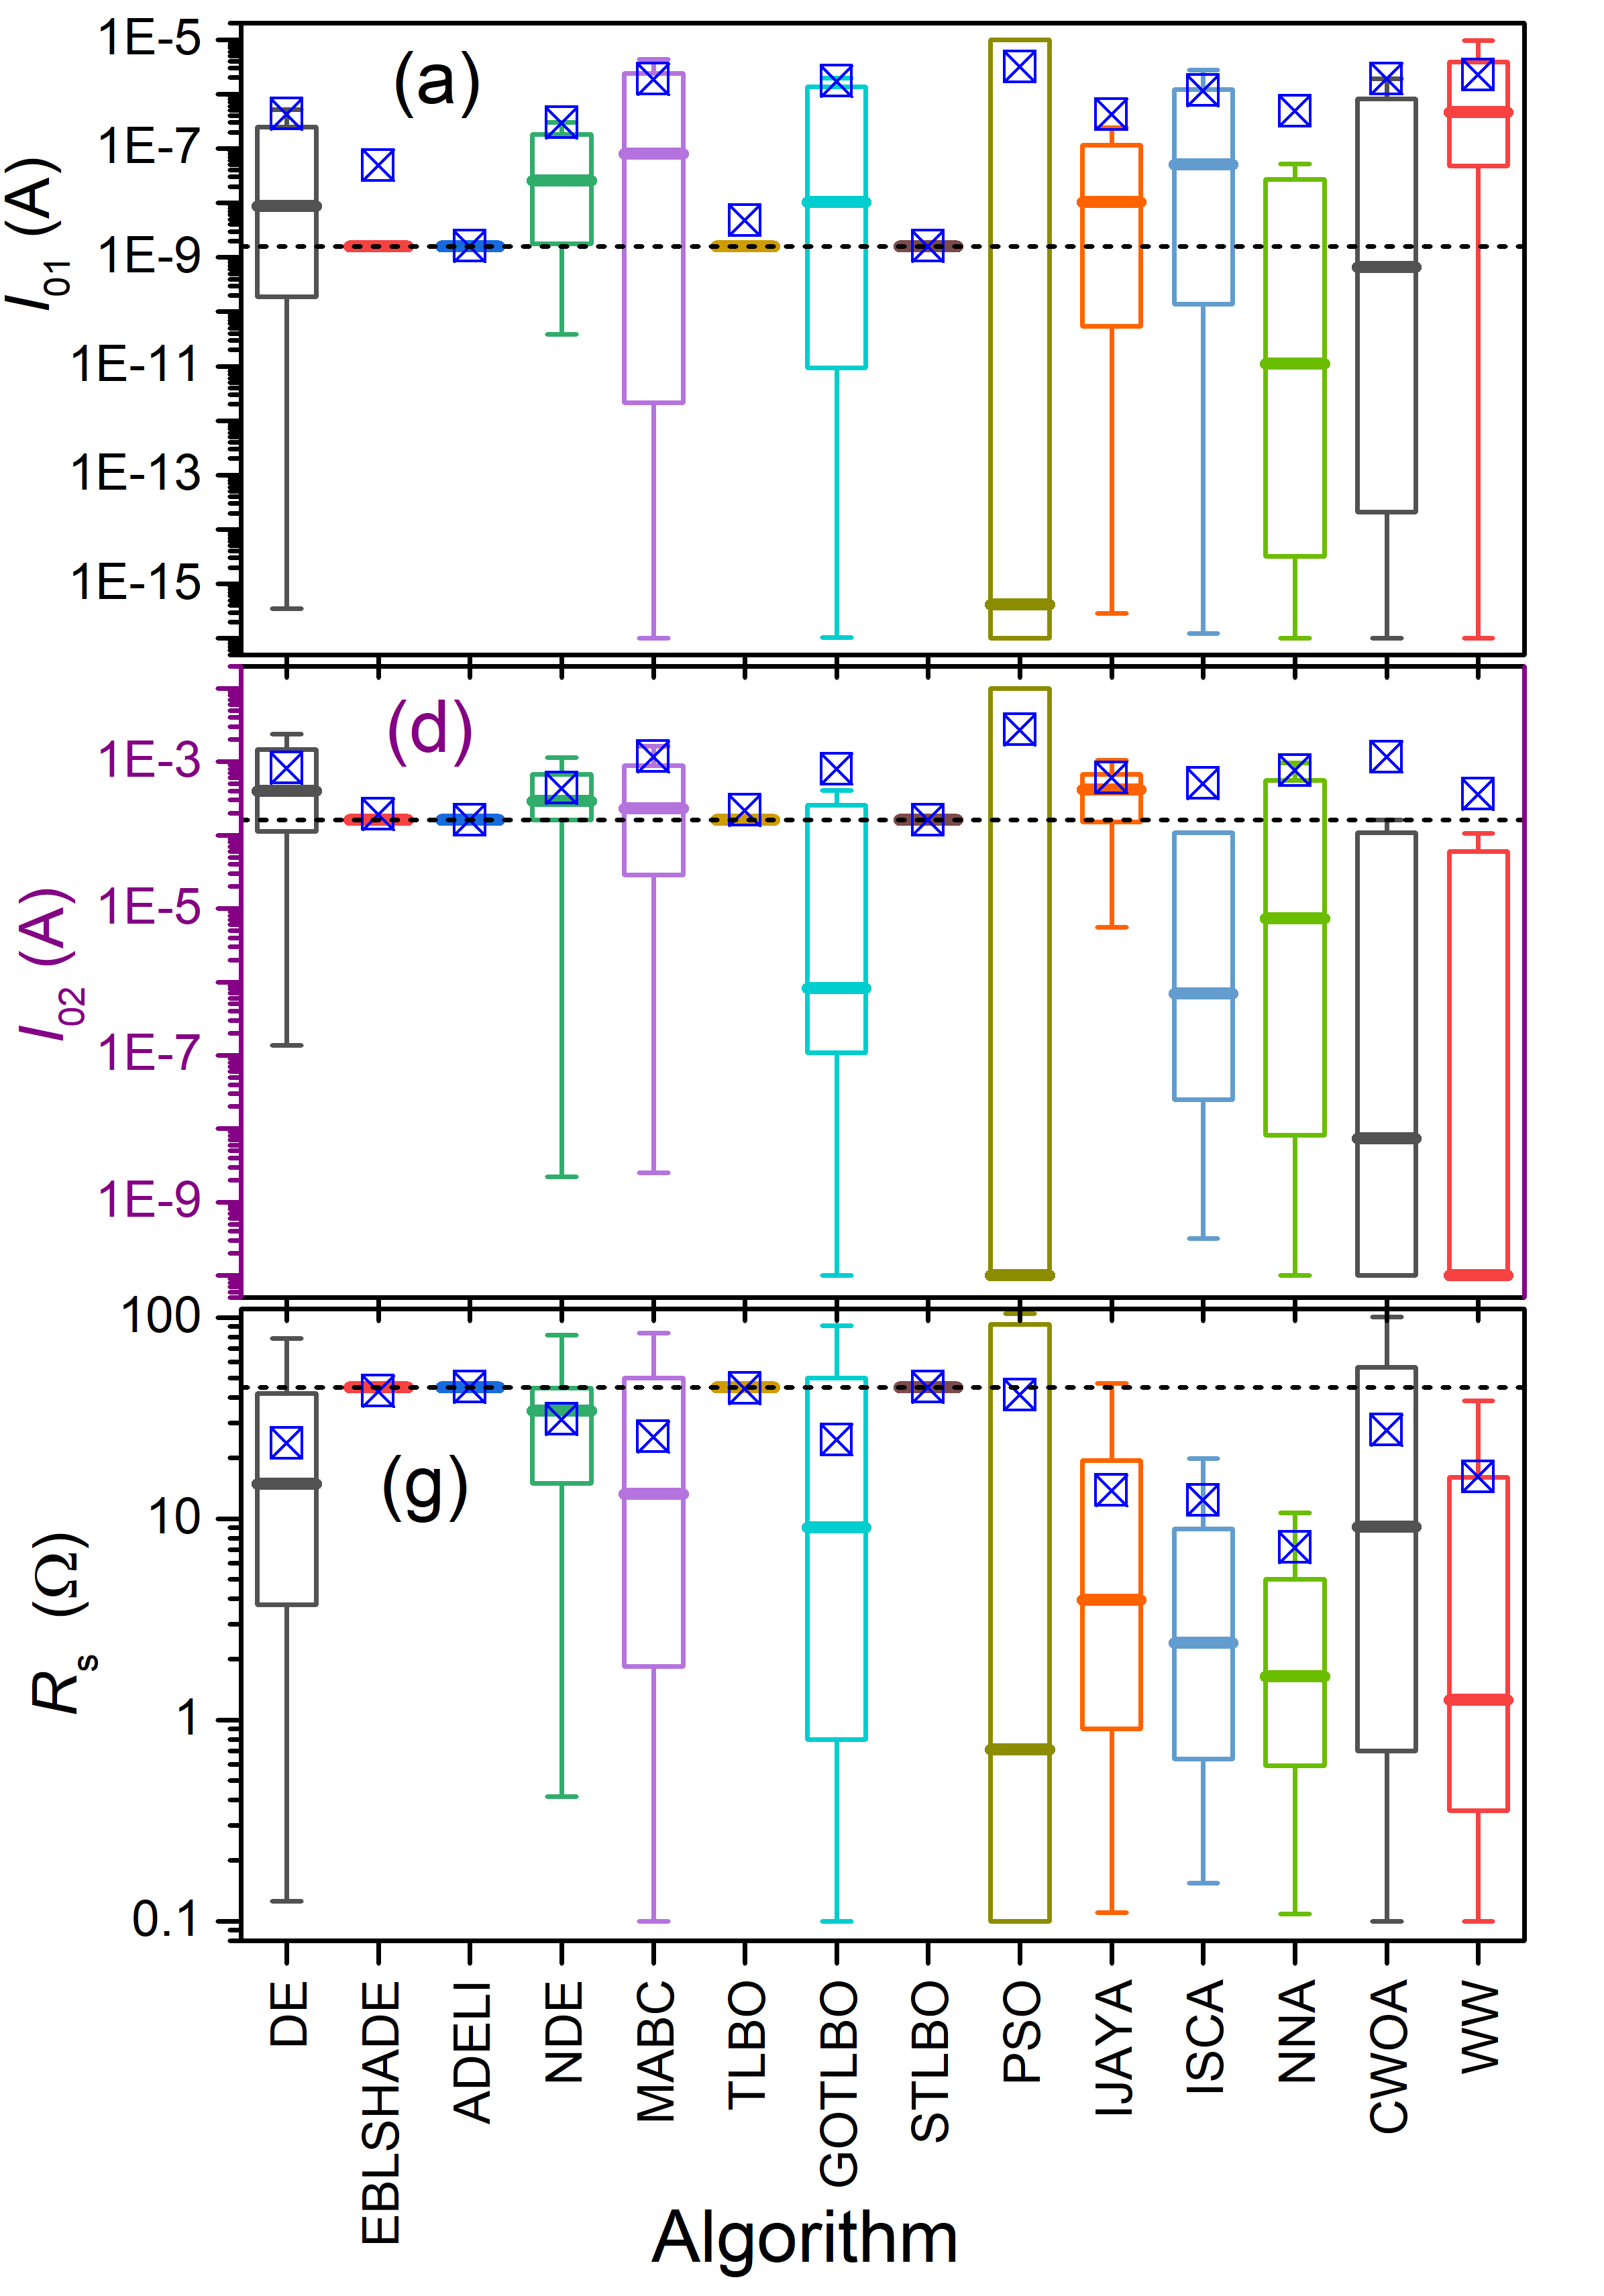
\includegraphics[width=.32\textwidth]{Fig3a}
        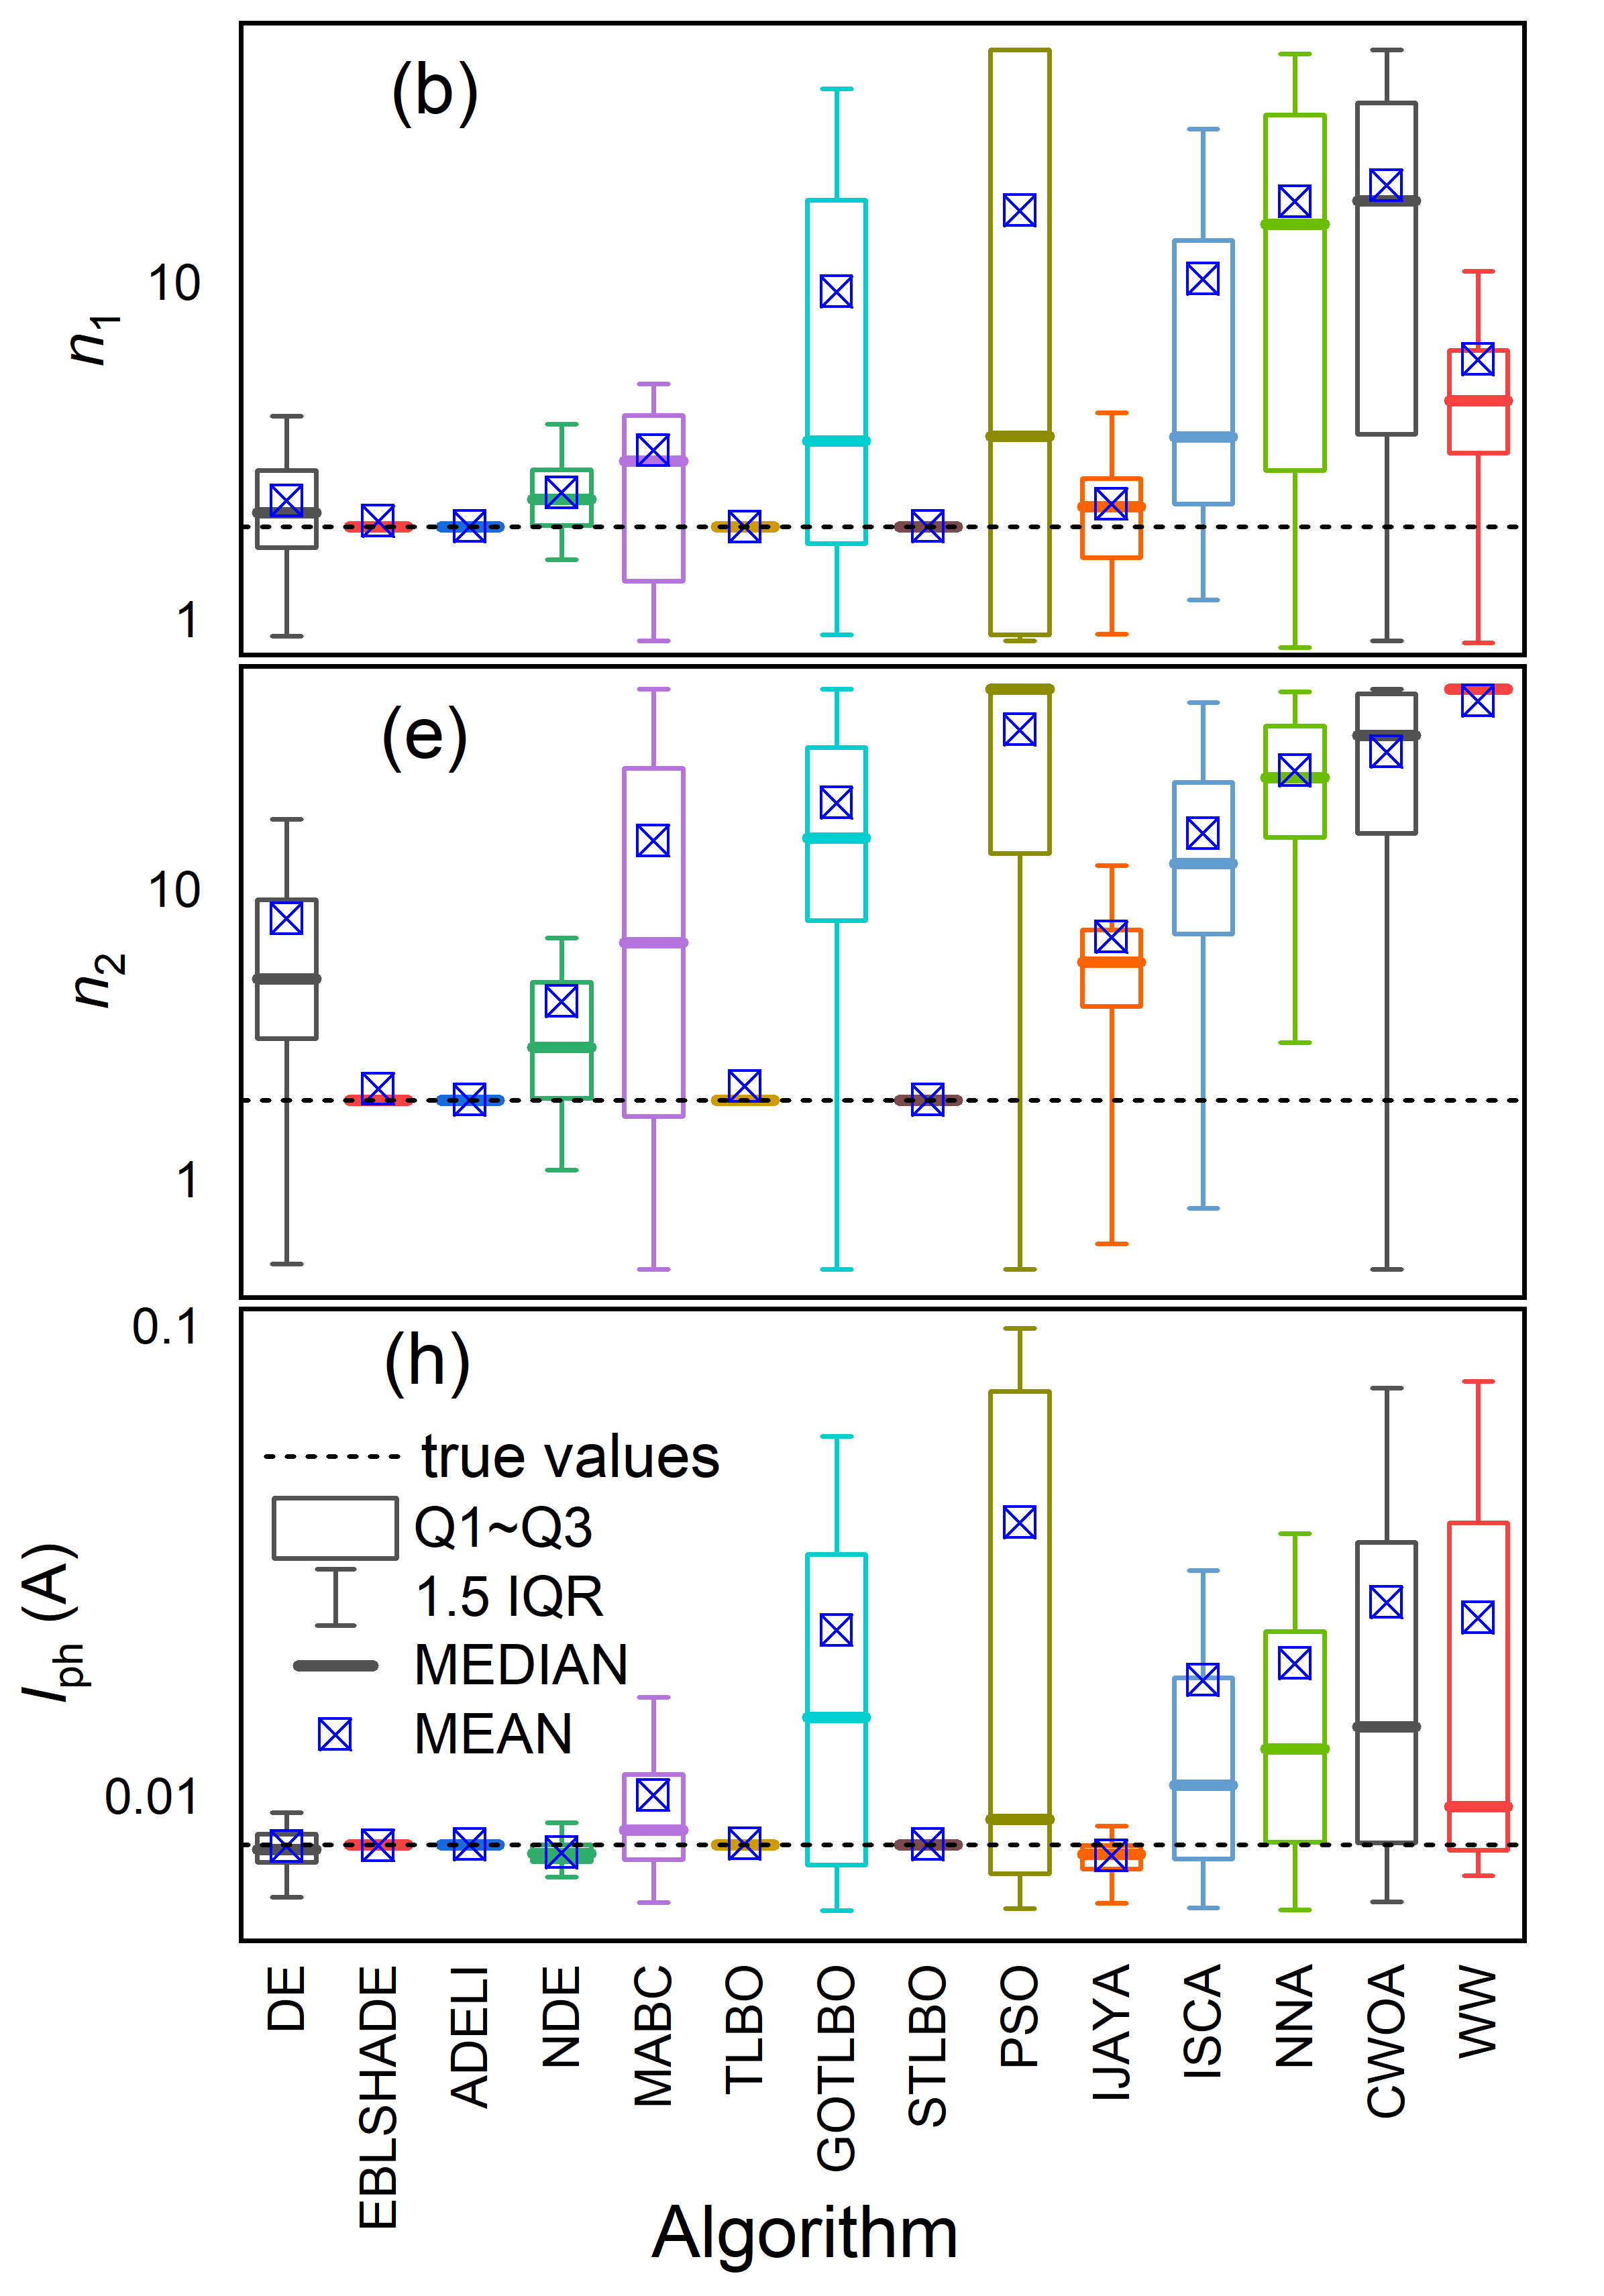
\includegraphics[width=.32\textwidth]{Fig3b}
        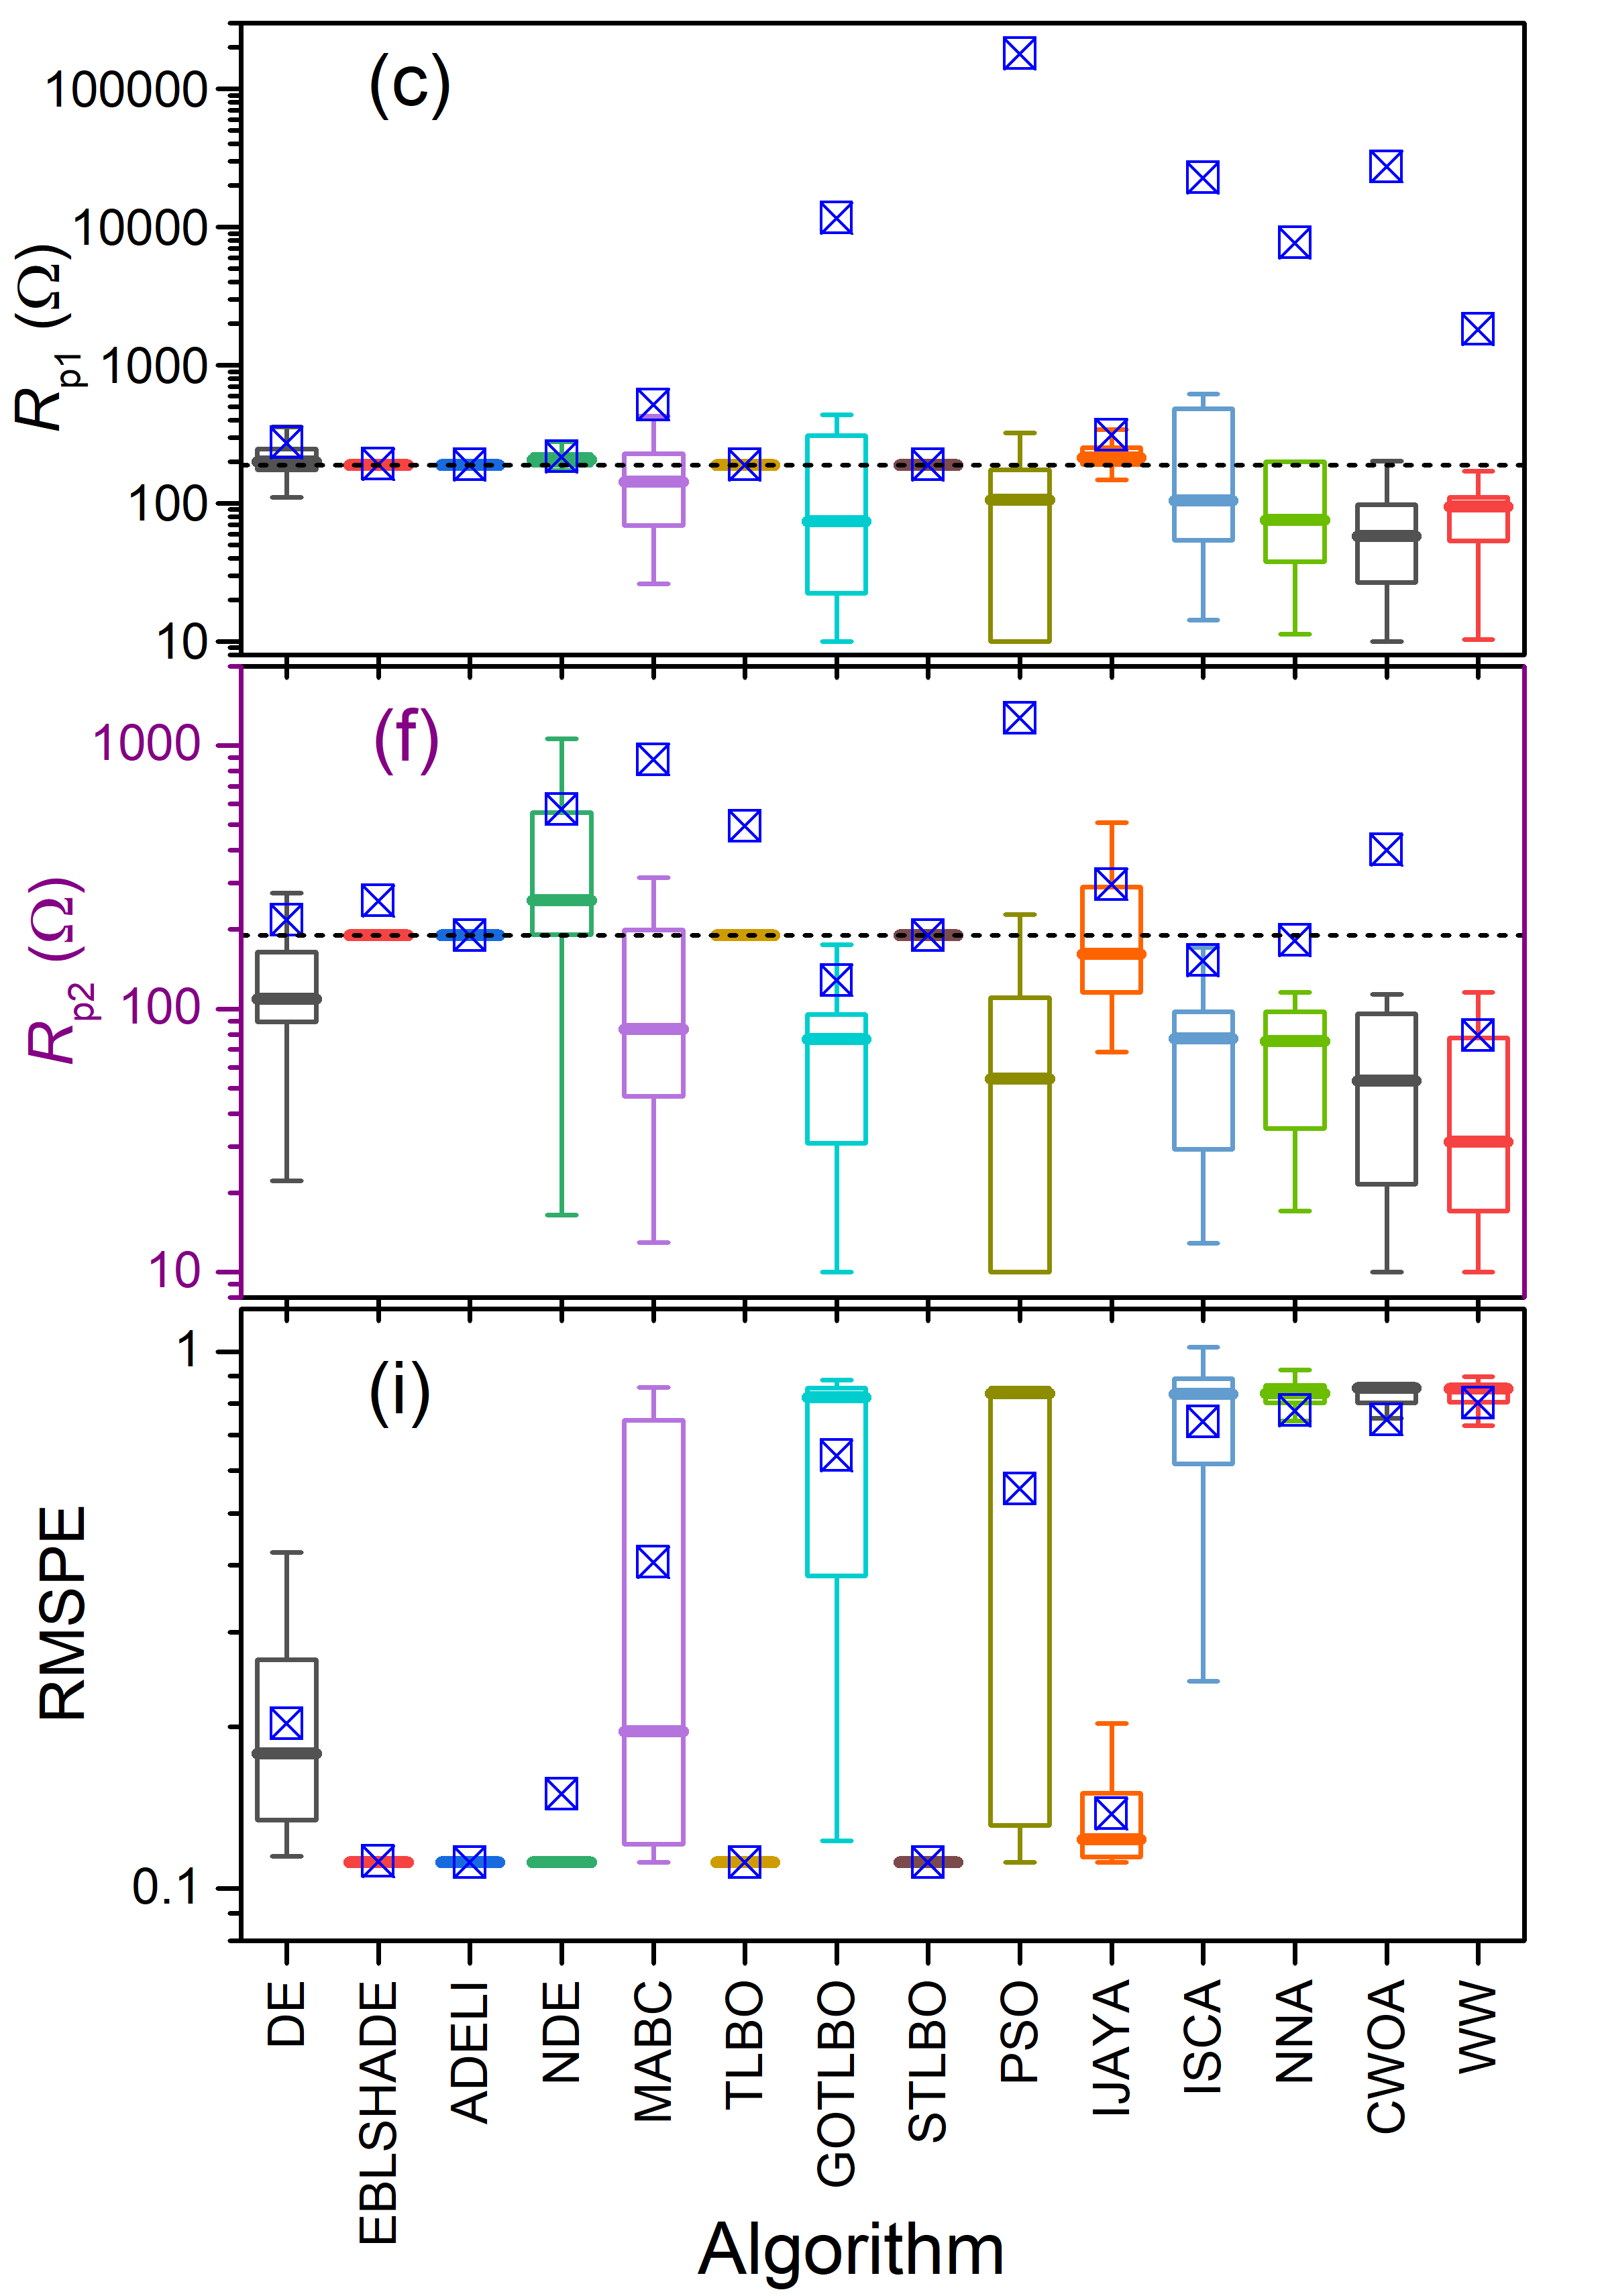
\includegraphics[width=.32\textwidth]{Fig3c}
	  \caption{Box--plot of  two--diode model parameter estimation from single IV curve using different optimizers.
      The squares are the mean values, and the dashed lines correspond to the true parameter values.}\label{figBoxSingleIV}
\end{figure*}

We would like to stress the following.
In most cases, median values are more relevant to the actual parameter values than the mean values.
Possible exceptions only apply to the estimation of $R_\mathrm{s}$ and $R_\mathrm{p2}$ only.
However, in cases where a method allows for parameter estimation with high accuracy (EBLSHADE, ADELI, TLBO, and STLBO),
MEDIANs are at least as good as the MEANs.
As a result, we will utilize median values as a robust measure of central tendency in nonparametric statistical tests.
Secondly, the increase in algorithm stability (reduction in STD and IQR values) in determining each model parameter correlates with the accuracy of parameter estimation.
Furthermore, IQR values are generally no worse than STD values.
Finally, small RMSPE values (close match between the fitting curve and the IV points)
do not always indicate high accuracy in determining the parameters of a solar cell --- see IJAYA and NDE data.
For example, the difference between the $\mathrm{MEDIAN}_\mathrm{RMSPE}$ values for NDE and ADELI is approximately 0.0001
(about 0.08\% of their absolute value).
At the same time, in the ADELI case, the values of $\mathrm{APE}_\mathrm{MEDIAN}$ do not exceed $6\cdot 10^{-4}$
for all model parameters estimation,
whereas for the NDE algorithm application, the obtained $\mathrm{APE}_\mathrm{MEDIAN}$ values are significantly higher
and range from 0.04 for $I_\mathrm{ph}$ to 11.4 for $I_{01}$.
On one hand, this confirms the issue identified by Tada \cite{Tada2015Organic,Tada2021}, which arises when estimating
parameters according to the opposed two--diode model from similar IV curves corresponding to photovoltaic cells with distinct characteristics.
Furthermore, the results indicate that some metaheuristic algorithms, such as NDE and IJAYA, can fall into a similar trap.
On the other hand, the high accuracy in parameter estimation demonstrated by EBLSHADE, ADELI, and STLBO indicates
that these algorithms are able to overcome the mentioned issue when applied.
It should be noted that a similar problem has been previously addressed by employing Bayesian estimation of parameters \cite{Tada2021}.
However, each Bayesian calculation took approximately half a day on a computer better equipped than ours \cite{Tada2021}.
In our case, when applying meta--heuristic algorithms, the worst--case run time did not exceed 100 seconds.

In order to statistically compare the algorithm under consideration, we use nonparametric tests.
In the single--IV case, all nonparametric statistical tests were used to compare the performance of meta--heuristic algorithms in assessing each of the eight model parameters.
The $\mathrm{APE}_i$ values were used, and the number of case problems in the study $N_\mathrm{pr}$ was equal to $N_\mathrm{runs}=51$.
Additionally, algorithms were compared in terms of curve-fitting accuracy by using RMSPE values.
Furthermore, tests were employed for a composite parameter as well.
This parameter, referred to as ``Comp'' hereafter, includes $\mathrm{APE}_\mathrm{MEDIAN}$ for each of the eight defined model parameters,
the median value for RMSPE, and $t_\mathrm{run}$.
This parameter may provide the most valuable insights for comparing algorithms. However, it is important to note that the value of $N_\mathrm{pr}$ is only 10.
According to Derrac \emph{et al} \cite{Derrac2011}, the number of case problems should be $N_\mathrm{pr}\geq 2k$,
where $k$ is the number of algorithms ($k=14$ in our study).
Therefore, the use of the Comp parameter is not strictly rigorous.
Indeed, it would have been possible to increase the $N_\mathrm{pr}$ value using, for example, $\mathrm{APE}_\mathrm{MEAN}$.
However, considering the deliberate utilization of a suboptimal parameter would have appeared inappropriate.



\begin{figure}[]
	\centering
		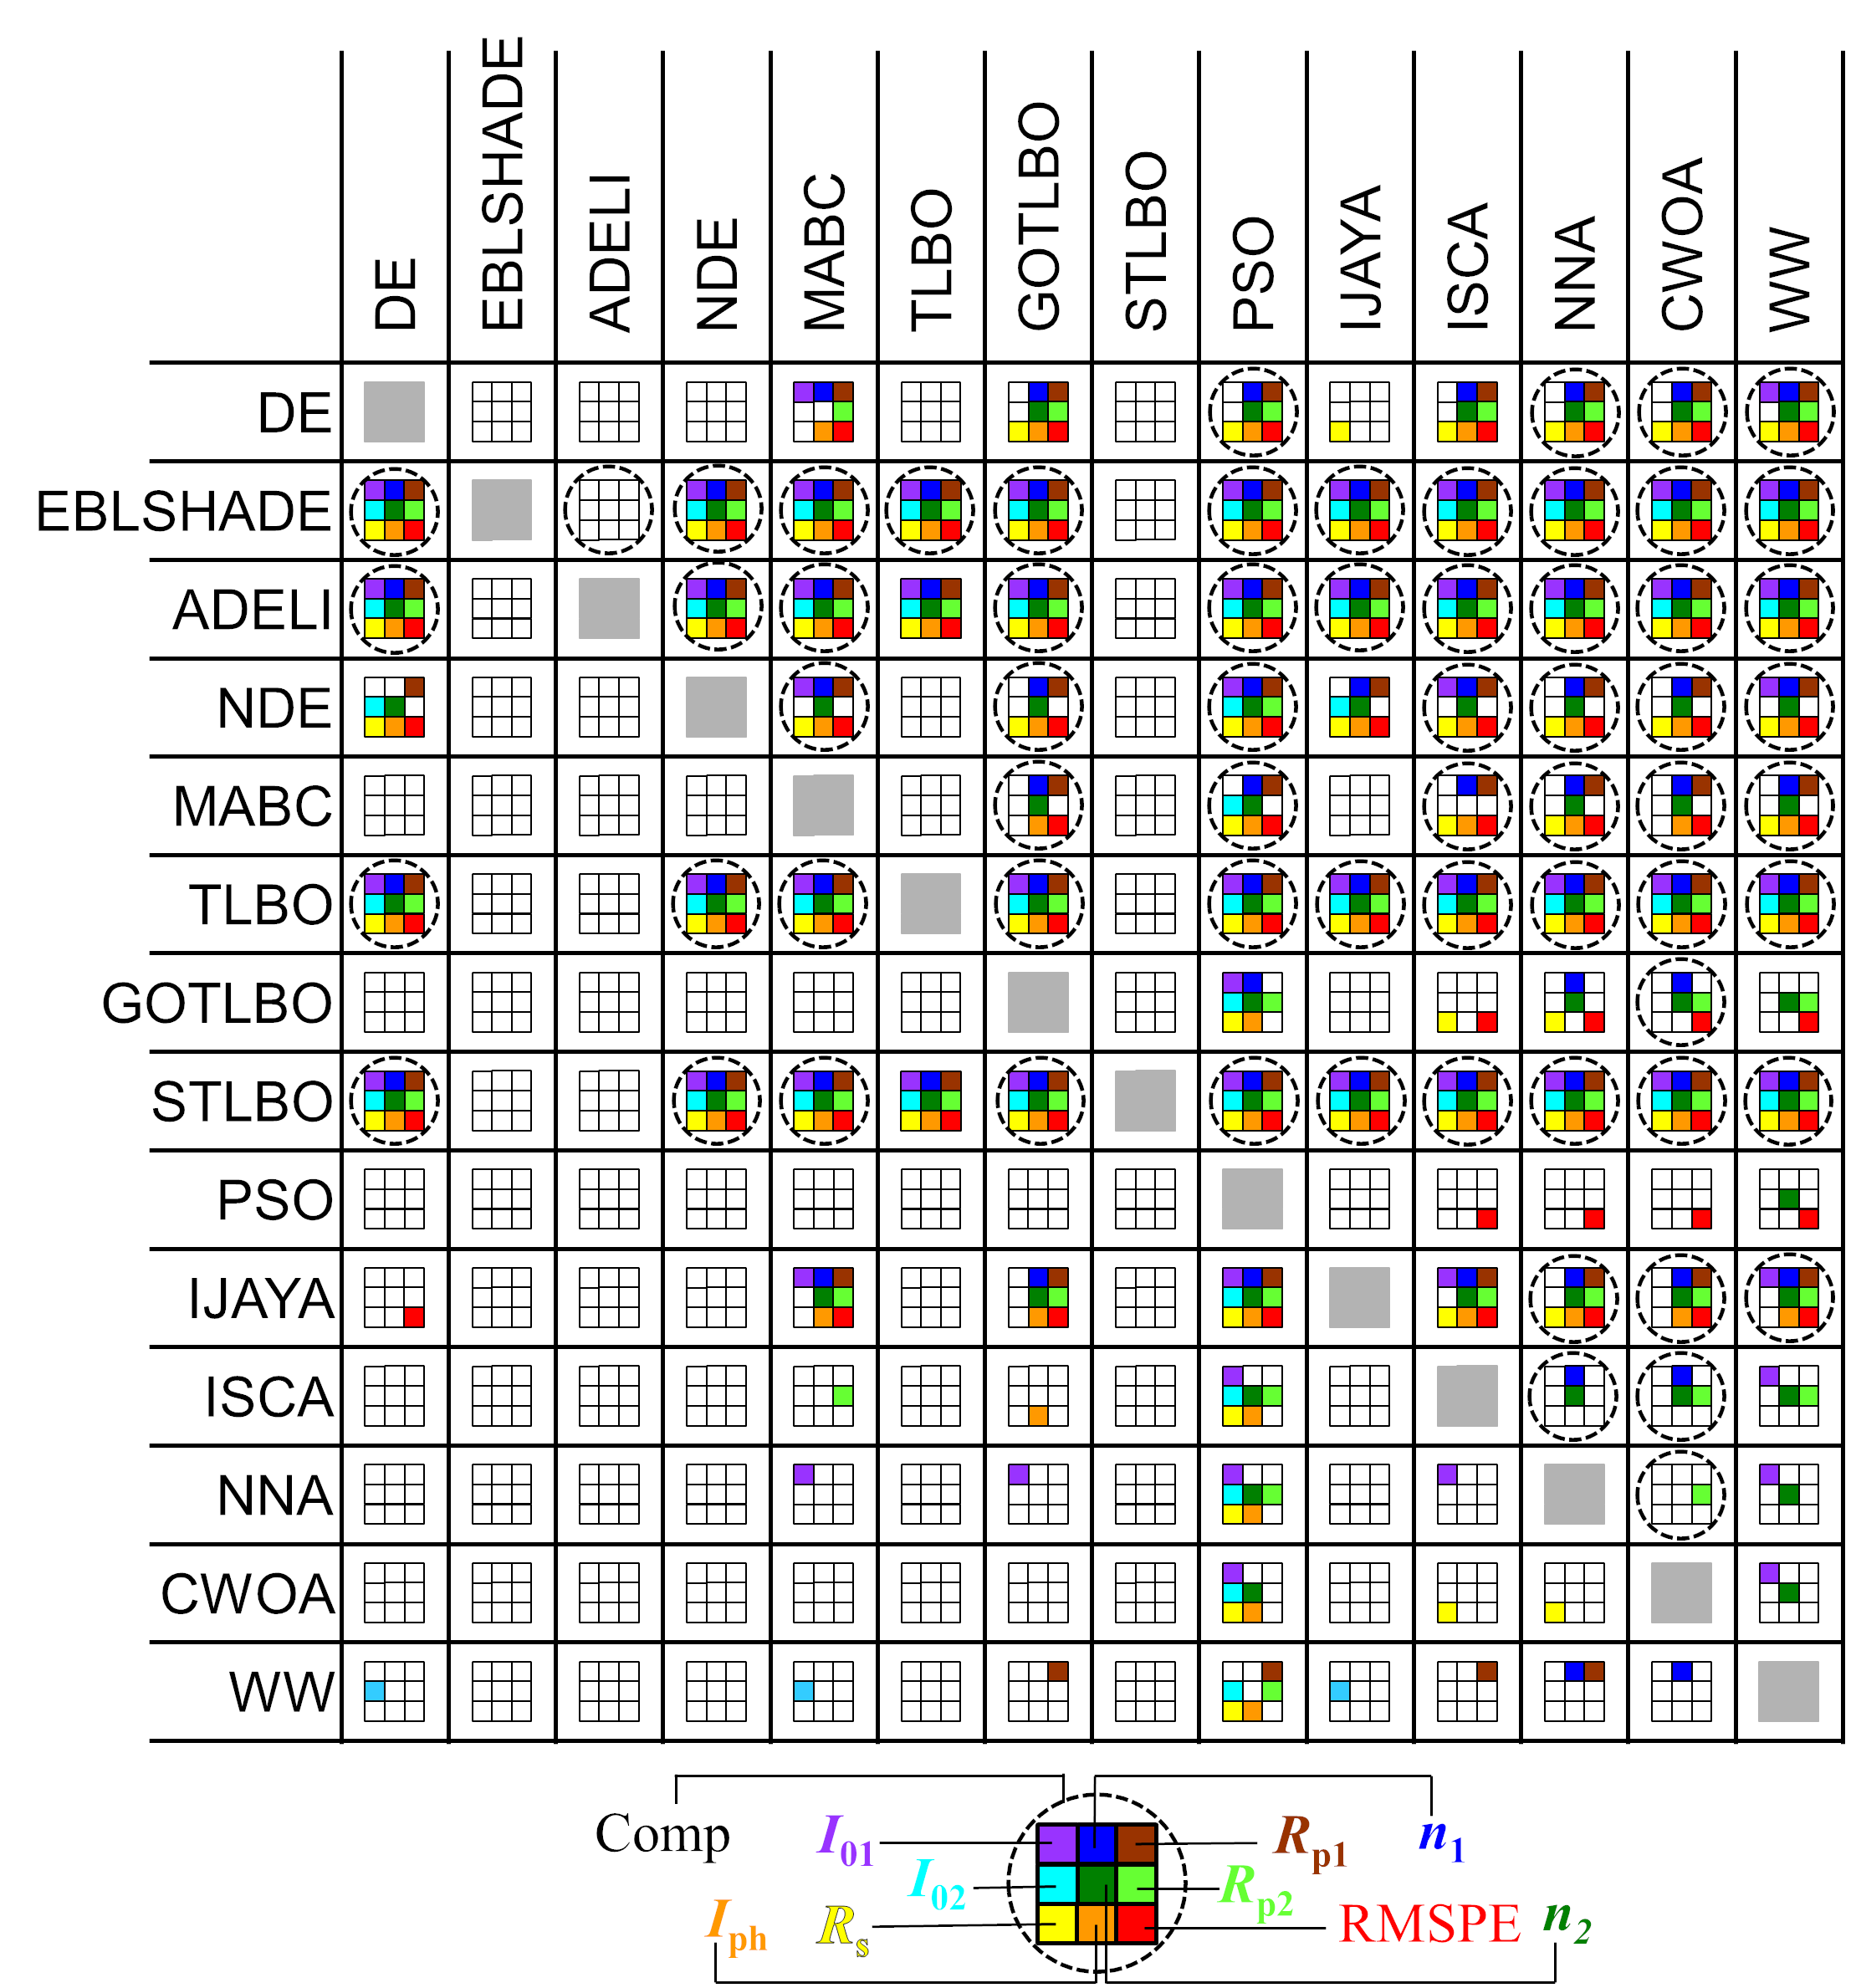
\includegraphics[width=1.0\columnwidth]{Fig4}
	  \caption{The results of Wilcoxon signed-rank test with a level of significance $\alpha = 0.05$ in the single-IV case.
               Each colored small square indicates that the algorithm specified in the row outperforms the algorithm
               specified in the column in evaluating one of the parameters of the two--diode model.
               The correspondence between the color and position of the square to a model parameter
               is shown in a legend at the figure bottom.
               The advantage of the row algorithm in the Comp parameter is indicated by the presence of a dashed circle.}\label{figWilSingleIV}
\end{figure}

\begin{figure}[]
	\centering
		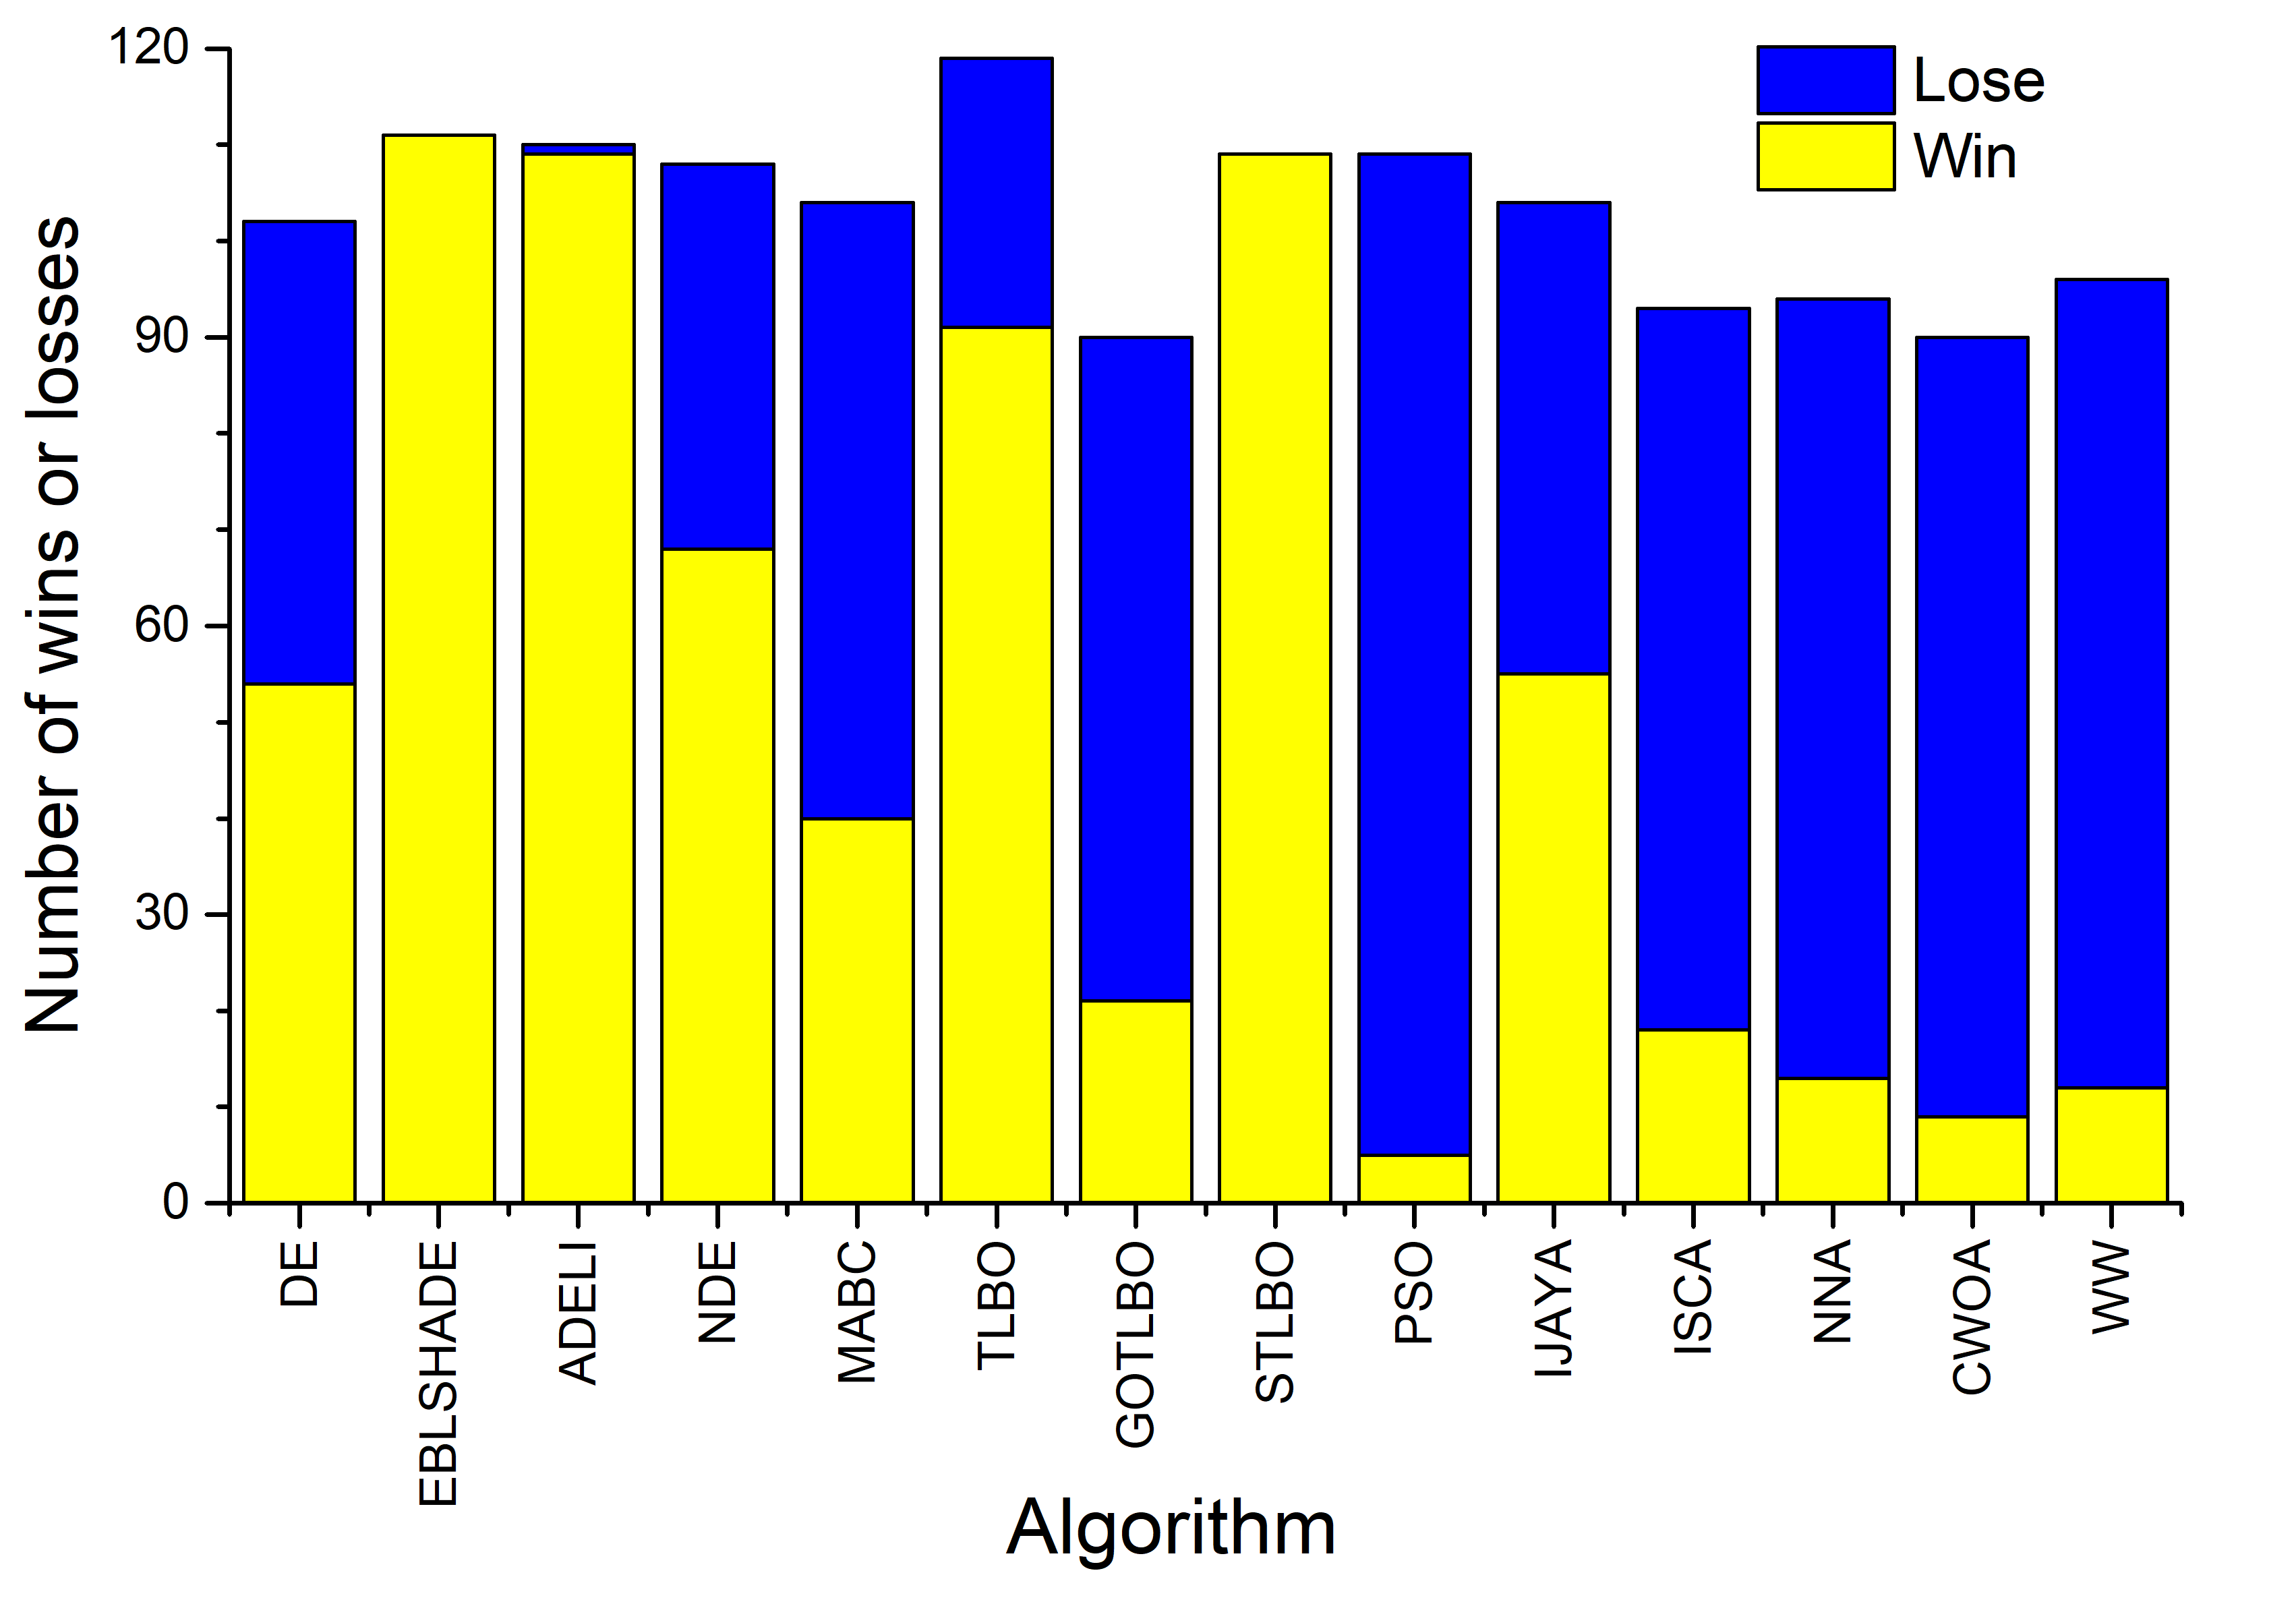
\includegraphics[width=1.0\columnwidth]{Fig5}
	  \caption{The total count of wins and losses for each algorithm in pairwise comparisons using the
               Wilcoxon signed-rank test with a significance level of $\alpha = 0.05$ in the single-IV case.}\label{figWilTotSingleIV}
\end{figure}




Fig.~\ref{figWilSingleIV} graphically show
the non--parametric statistical results of pairwise comparisons of algorithms
based on the Wilcoxon signed--rank test.
In the case of Comp comparisons, the differences in performance scores
were normalized to the interval $[0,\, 1]$.
As seen from the figure, no algorithm outperforms all others in evaluating each parameter.
Furthermore, no algorithm surpasses all others in the estimation even a single parameter.
For example, as the figure states, STLBO shows a significant improvement over
DE, NDE, MABC, GOTLBO, PSO, IJAYA, ISCA, NNA, CWOA, and WW across all the parameters considered
with a level of significance $\alpha = 0.05$.
Simultaneously, it was not detected the significant differences
between STLBO and both EBLSHADE and ADELI for all parameter estimations
as well as between STLBO and TLBO in the Comp case.
EBLSHADE outperforms nearly all other algorithms in the composite parameter, except for STLBO.
According to the Wilcoxon test victories count,
the worst performances are exhibited by PSO and CWOA.
PSO achieved better results than ISCA, NNA, and CWOA in terms of RMSPE value,
as well as outperformed WW in $n_2$ estimation and RMSPE.
Test detected significant differences between CWOA and WW in $n_2$ and $I_{01}$ estimations,
between CWOA and PSO in $I_{01}$, $I_{02}$, $R_\mathrm{s}$, and $I_\mathrm{ph}$ estimations),
and between CWOA and both ISCA and NNA in $R_\mathrm{s}$  estimation case only.


Looking at the results of the Wilcoxon signed-rank test from another perspective,
it can be observed that neither EBLSHADE nor STLBO had any defeats in pairwise comparisons,
while ADELI had only one loss.
ADELI was only outperformed by EBLSHADE in terms of the Comp parameter, primarily due to its significantly longer run time.
The highest count of defeats was observed for the PSO and WW algorithms (104 and 84, respectively).
The data regarding the total count of wins and losses when applying the Wilcoxon test
for each algorithm are summarized in Fig.~\ref{figWilTotSingleIV}.

\begin{figure}[!ht]
	\centering
		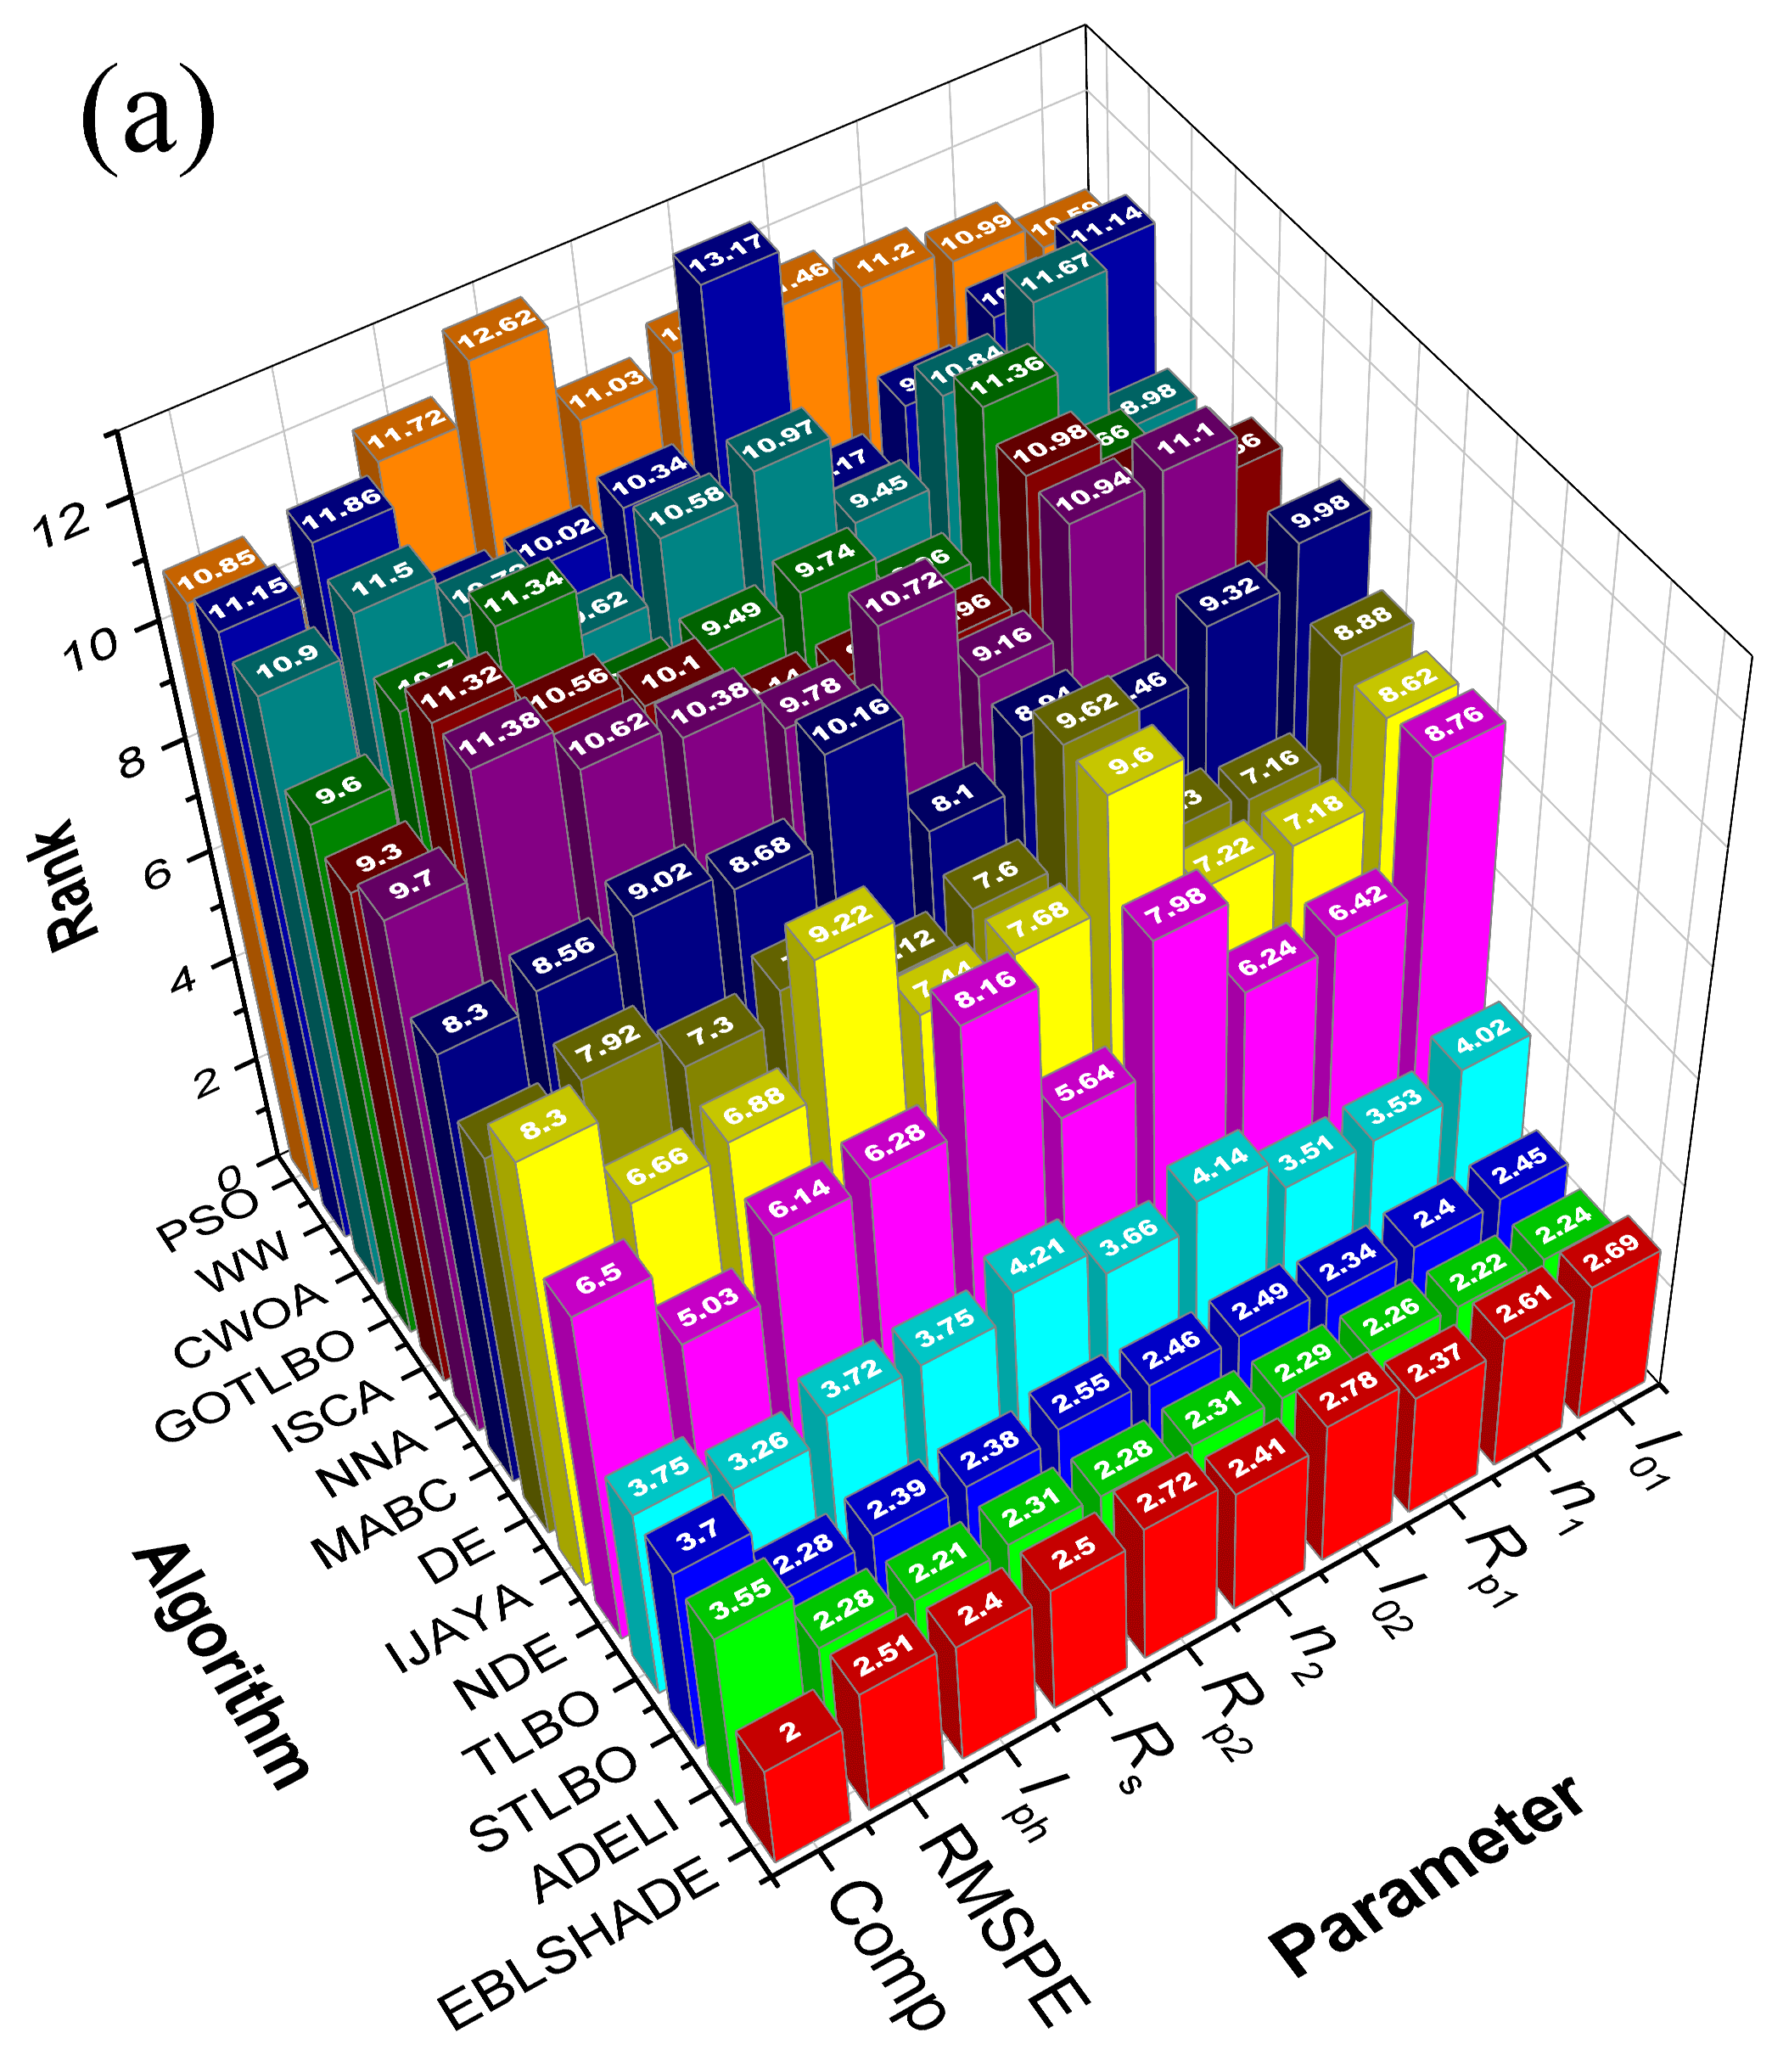
\includegraphics[width=.76\columnwidth]{Friedman}
        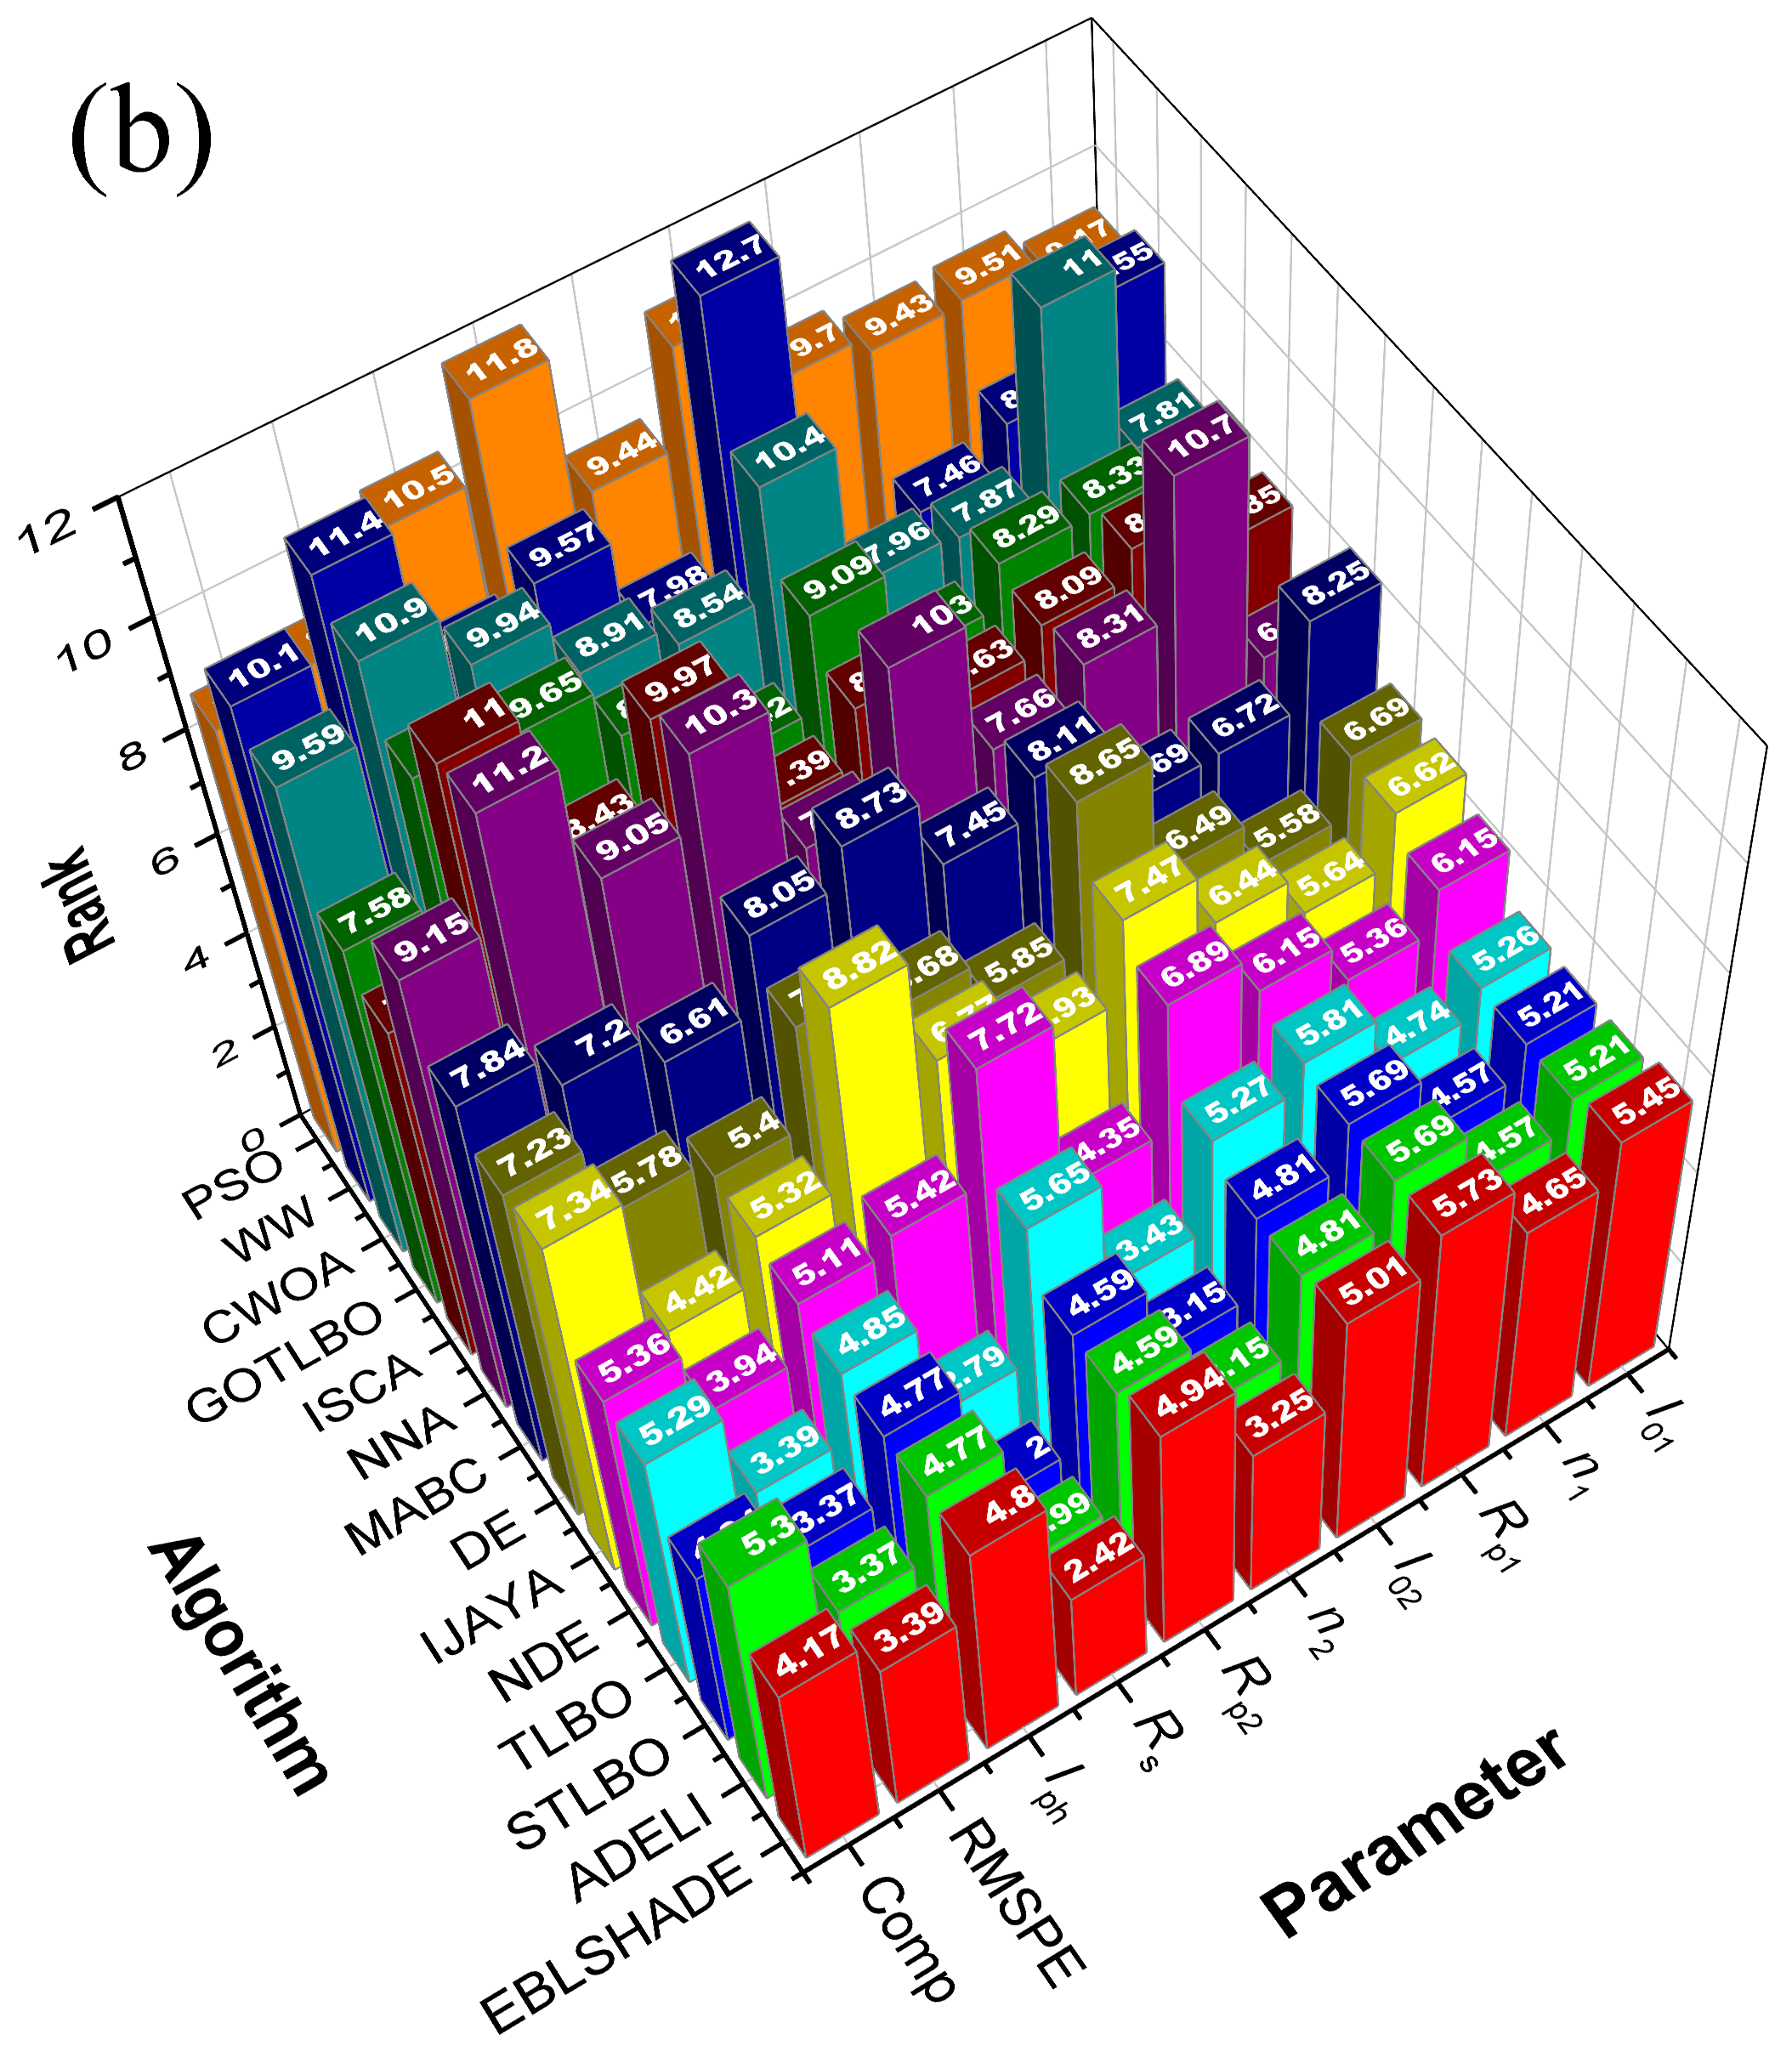
\includegraphics[width=.76\columnwidth]{FriedmanAlignedRank}
        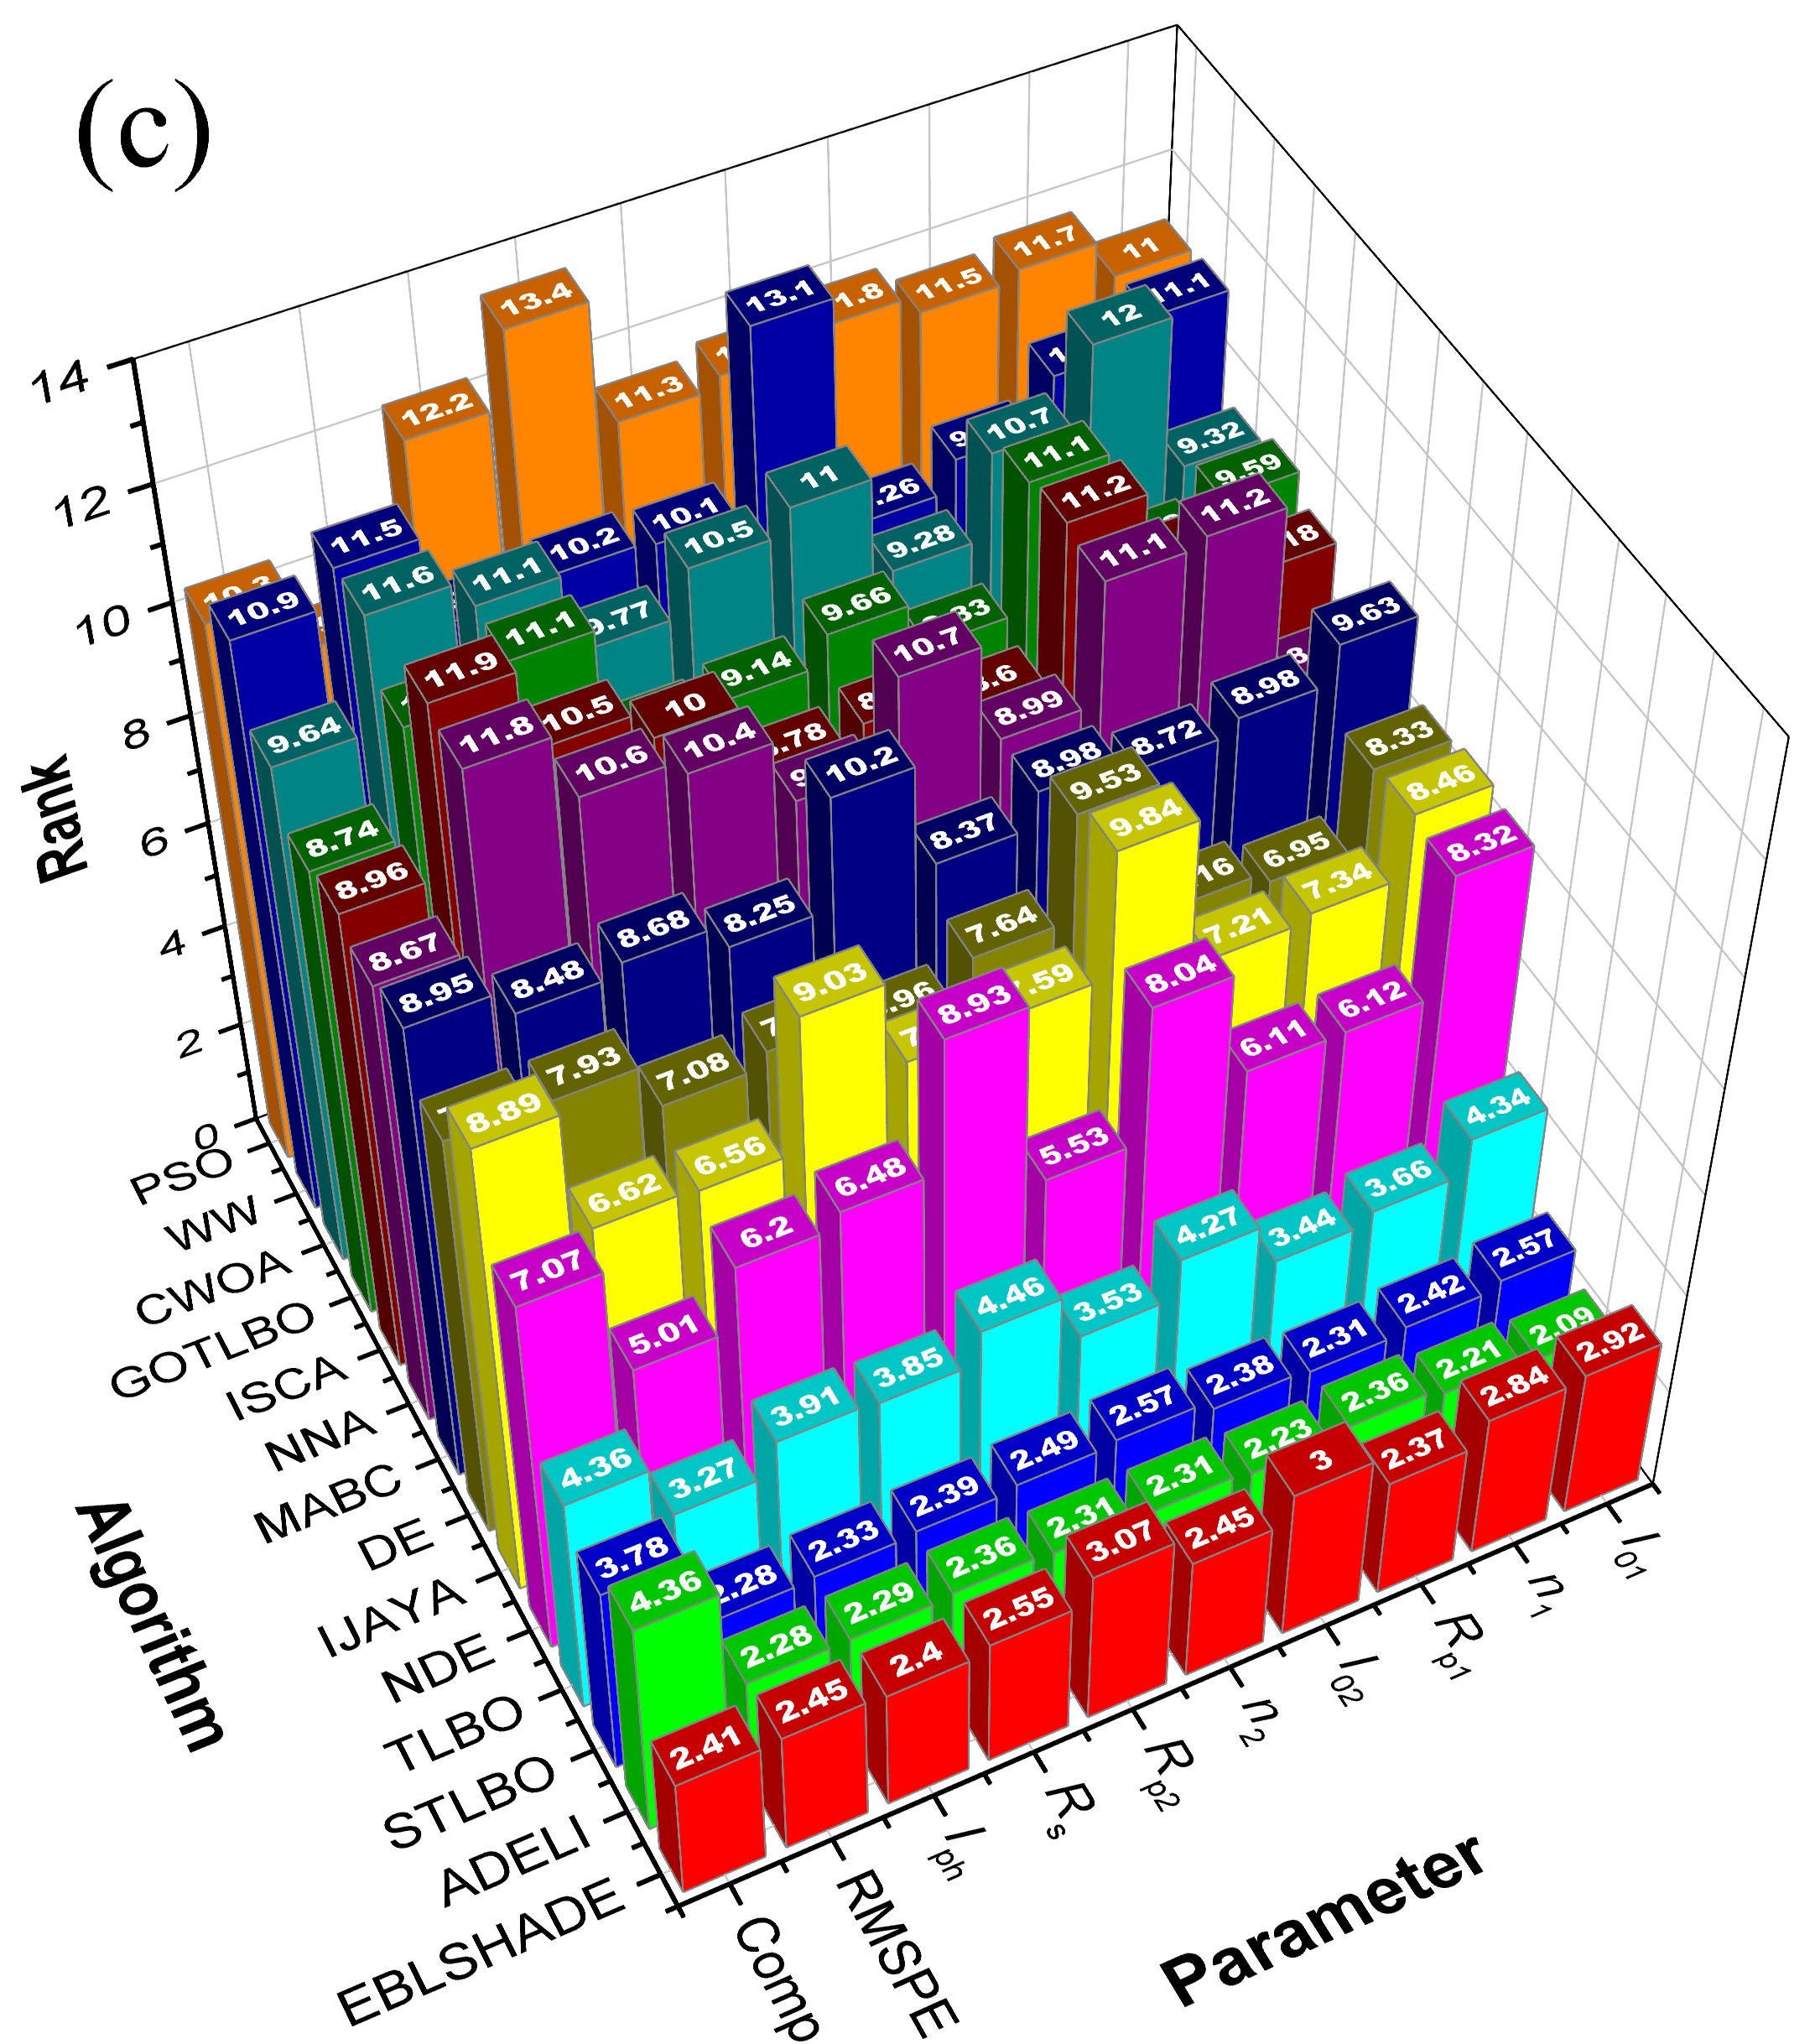
\includegraphics[width=.76\columnwidth]{QuadeRank}
	  \caption{Ranking of the algorithms according to Friedman (a), Friedman Aligned (b), and Quade (c) tests in the single-IV case.}\label{figRanksSingleIV}
\end{figure}

It is recommended \cite{Derrac2011} to begin the multiple comparisons tests by examining the null hypothesis $H_0$,
which asserts the equality of medians between the populations of results obtained by different algorithms.
The null hypothesis $p$--values computed through the statistics of  Friedman, Friedman Aligned, and Quade test
and the Iman–Davenport extension
are given in the supplementary material (table S2).
The highest observed $p(H_0)$--values were found to be $2.7\cdot10^{-5}$ (Friedman Aligned test for the task of $R_\mathrm{p1}$ estimation),
$4.4\cdot10^{-4}$ (Friedman Aligned test for the composite parameter case),
and $8.3\cdot10^{-6}$ (Quade test, Comp parameter).
Thus obtained data strongly suggest the existence of significant differences
among the considered algorithms in the accuracy of all model parameter determination, RMSPE values, and Comp parameter.



Fig.~\ref{figRanksSingleIV} shows
ranks achieved by the Friedman, Friedman Aligned, and Quade tests for applied optimization algorithms in different tasks.
Ranks are tabulated in the supplementary material as well (table S3).
In almost all cases, the algorithms EBLSHADE, ADELI, and STLBO consistently achieve the top (smallest value) three ranks.
For example, in assessing the accuracy of model parameter estimation, ADELI has ranked first 22 times.
The STLBO algorithm ranked first six times,
taking the sole first place twice ($I_{01}$ estimation according Friedman Aligned test and
$R_\mathrm{p1}$ estimation according Quade test)
and sharing it with ADELI four times ($n_1$, $R_\mathrm{p1}$, $n_2$, and $I_\mathrm{ph}$ estimation according Friedman Aligned test).
In the RMSPE value case, ADELI and STLBO achieved equal and best ranks by all three used tests.
When comparing based on the Comp parameter,
the STLBO algorithm obtained the top rank according to the Friedman Aligned test,
while the Friedman and Quade tests recognized EBLSHADE as the best.
In most cases, the TLBO algorithm secured the fourth position, and in four cases, it even ranked third.
In the majority of cases, the TLBO algorithm consistently ranked fourth out of all the algorithms tested.
Interestingly, in four cases ($I_{01}$ estimation, RMSPE value, and Comp parameter by Friedman Aligned test,
and Comp parameter by Quade test),
it even achieved a commendable third-place ranking.
We must note that overall, the absolute values of ranks for ADELI, STLBO, EBLSHADE and TLBO algorithms differ little,
and the difference between the first and fourth ranks is often less than 0.5.
The worst ranks are observed for PSO, NNA, CWOA, and WW.

It is known \cite{Derrac2011} that
the Friedman, Friedman Aligned, and Quade tests are insufficient in establishing accurate comparisons between the algorithms considered.
To compare a control method (1 of 14 compared) with a set of other algorithms (rest 13),
one can define a family of hypotheses related to the control method.
Applying a post-hoc test makes it possible to obtain a $p$--value that indicates the extent to which each hypothesis can be rejected.
We calculated $p$--values using four post-hoc procedures (Finner, Holm, Hochberg, and Holland) for all algorithms, tests, and tasks.
By following the indications given for the four post-hoc procedures considered, Table~\ref{tbl1NADELI} shows the $p$--values
obtained, using the ranks computed by the Friedman, Friedman Aligned, and Quade tests for the case of control algorithm ADELI
and the task of $R_\mathrm{p1}$ estimation.
These are typical results, the reader is referred to the supplementary material for rest of $p$-values (Tables S4-S143).


\begin{table*}[<options>]
\caption{Adjusted $p$-values for Friedman, Friedman Aligned, and Quade tests in single--IV case.
 ADELI is the control algorithm, and the task of $R_\mathrm{p1}$ estimation is under consideration.}\label{tbl1NADELI}
\begin{tabular*}{\tblwidth}{@{}LLCCCC@{}}
\toprule
\multirow{2}{*}{Algorithm}& \multirow{2}{*}{Test}& \multicolumn{4}{C}{post-hoc procedure} \\
  & &Finner & Holm & Hochberg &Holland\\ % Table header row
\midrule
GOTLBO&	Friedman&<1E-13&<1E-13&<1E-13&<1E-13\\
&Friedman Aligned&2.23361E-09&6.87266E-09&6.87266E-09&6.87266E-09\\
&Quade&2.57827E-03&4.09880E-03&3.90245E-03&4.09117E-03\\
PSO&Friedman&<1E-13&<1E-13&<1E-13&<1E-13\\
&Friedman Aligned&<1E-13&<1E-13&<1E-13&<1E-13\\
&Quade&2.57827E-03&2.58134E-03&2.58134E-03&2.57827E-03\\
MABC&Friedman&6.35048E-13&1.61204E-12&1.61204E-12&1.61204E-12\\
&Friedman Aligned&7.88131E-06&2.97065E-05&2.97065E-05&2.97062E-05\\
&Quade&1.73550E-02&6.56791E-02&6.56791E-02&6.38590E-02\\
WW&Friedman&1.84926E-10&5.69003E-10&5.69003E-10&5.69003E-10\\
&Friedman Aligned&3.15599E-13&8.01137E-13&8.01137E-13&8.01137E-13\\
&Quade&5.31725E-03&1.96611E-02&1.96611E-02&1.94928E-02\\
DE&Friedman&4.61292E-09&1.59678E-08&1.59678E-08&1.59678E-08\\
&Friedman Aligned&3.62181E-04&1.33738E-03&1.33738E-03&1.33663E-03\\
&Quade&7.62673E-02&2.85885E-01&2.49968E-01&2.53918E-01\\
IJAYA&Friedman&6.88175E-09&2.54096E-08&2.54096E-08&2.54096E-08\\
&Friedman Aligned&8.79672E-04&3.04543E-03&3.04543E-03&3.04172E-03\\
&Quade&7.62673E-02&2.85885E-01&2.49968E-01&2.53918E-01\\
CWOA&Friedman&8.73483E-09&3.29236E-08&3.29236E-08&3.29236E-08\\
&Friedman Aligned&4.27917E-09&1.58000E-08&1.58000E-08&1.58000E-08\\
&Quade&2.57827E-03&5.93402E-03&5.93402E-03&5.91840E-03\\
NNA&Friedman&1.17491E-08&4.33811E-08&4.27586E-08&4.33811E-08\\
&Friedman Aligned&2.23361E-09&7.25937E-09&7.25937E-09&7.25937E-09\\
&Quade&2.57827E-03&4.09880E-03&3.90245E-03&4.09117E-03\\
ISCA&Friedman&1.23525E-08&4.33811E-08&4.27586E-08&4.33811E-08\\
&Friedman Aligned&<1E-13&<1E-13&<1E-13&<1E-13\\
&Quade&2.57827E-03&3.65691E-03&3.65691E-03&3.65079E-03\\
NDE&Friedman&2.55436E-06&7.85957E-06&7.85957E-06&7.85955E-06\\
&Friedman Aligned&4.19953E-02&1.29854E-01&1.29854E-01&1.23666E-01\\
&Quade&1.60056E-01&5.02233E-01&5.02233E-01&4.15313E-01\\
TLBO&Friedman&1.57702E-01&4.05499E-01&4.05499E-01&3.53159E-01\\
&Friedman Aligned&6.48054E-01&1.0&1.0&9.29409E-01\\
&Quade&7.18467E-01&1.0&1.0&9.59945E-01\\
EBLSHADE&Friedman&9.13338E-01&1.0&9.23824E-01&9.89059E-01\\
&Friedman Aligned&8.67482E-01&1.0&1.0&9.76034E-01\\
&Quade&9.98363E-01&1.0&1.0&9.99993E-01\\
STLBO&Friedman&9.23824E-01&1.0&9.23824E-01&9.89059E-01\\
&Friedman Aligned&1.0&1.0&1.0&1.0\\
&Quade&1.0&1.0&1.0&1.0\\
\bottomrule
\end{tabular*}
\end{table*}


As we can see in the table, the Finner post-hoc procedure exhibits the most powerful behavior,
reaching the lowest $p$-values in the comparisons.
The Friedman test shows a significant improvement in $R_\mathrm{p1}$ estimation of ADELI over
DE, NDE, MABC, GOTLBO, PSO, IJAYA, ISCA, NNA, CWOA, and WW
for all the post-hoc procedures considered.

The Friedman Aligned test only confirms the improvement of ADELI
over the aforementioned 10 algorithms for every post-hoc procedure considered,
except Holm, Hochberg, and Holland,
which fail to highlight the differences between ADELI and NDE as significant.

Finally, the Quade test find significant difference between ADELI and
MABC, GOTLBO, PSO, ISCA, NNA, CWOA, WW for every post-hoc procedure.
In the DE and IJAYA cases, ADELI obtains better results in $R_\mathrm{p1}$ estimation
according Finner post-hoc procedure only.
This result supports the conclusion that,
although ADELI outperforms the weaker algorithms of our study,
its performance differences are not significant when compared to other power algorithms (STLBO, EBLSHADE, TLBO).

In our study, a threshold value of $p_{cr}=0.1$ was adopted to establish a critical level
for comparing the effectiveness of two algorithms in both multiple $1\times N$ and $N\times N$ comparisons.
That is, it was determined that the likelihood of obtaining a result as extreme as the observed one,
under the assumption that there is no difference between the two algorithms (null hypothesis), was less than 10\%.



\begin{figure*}[]
	\centering
		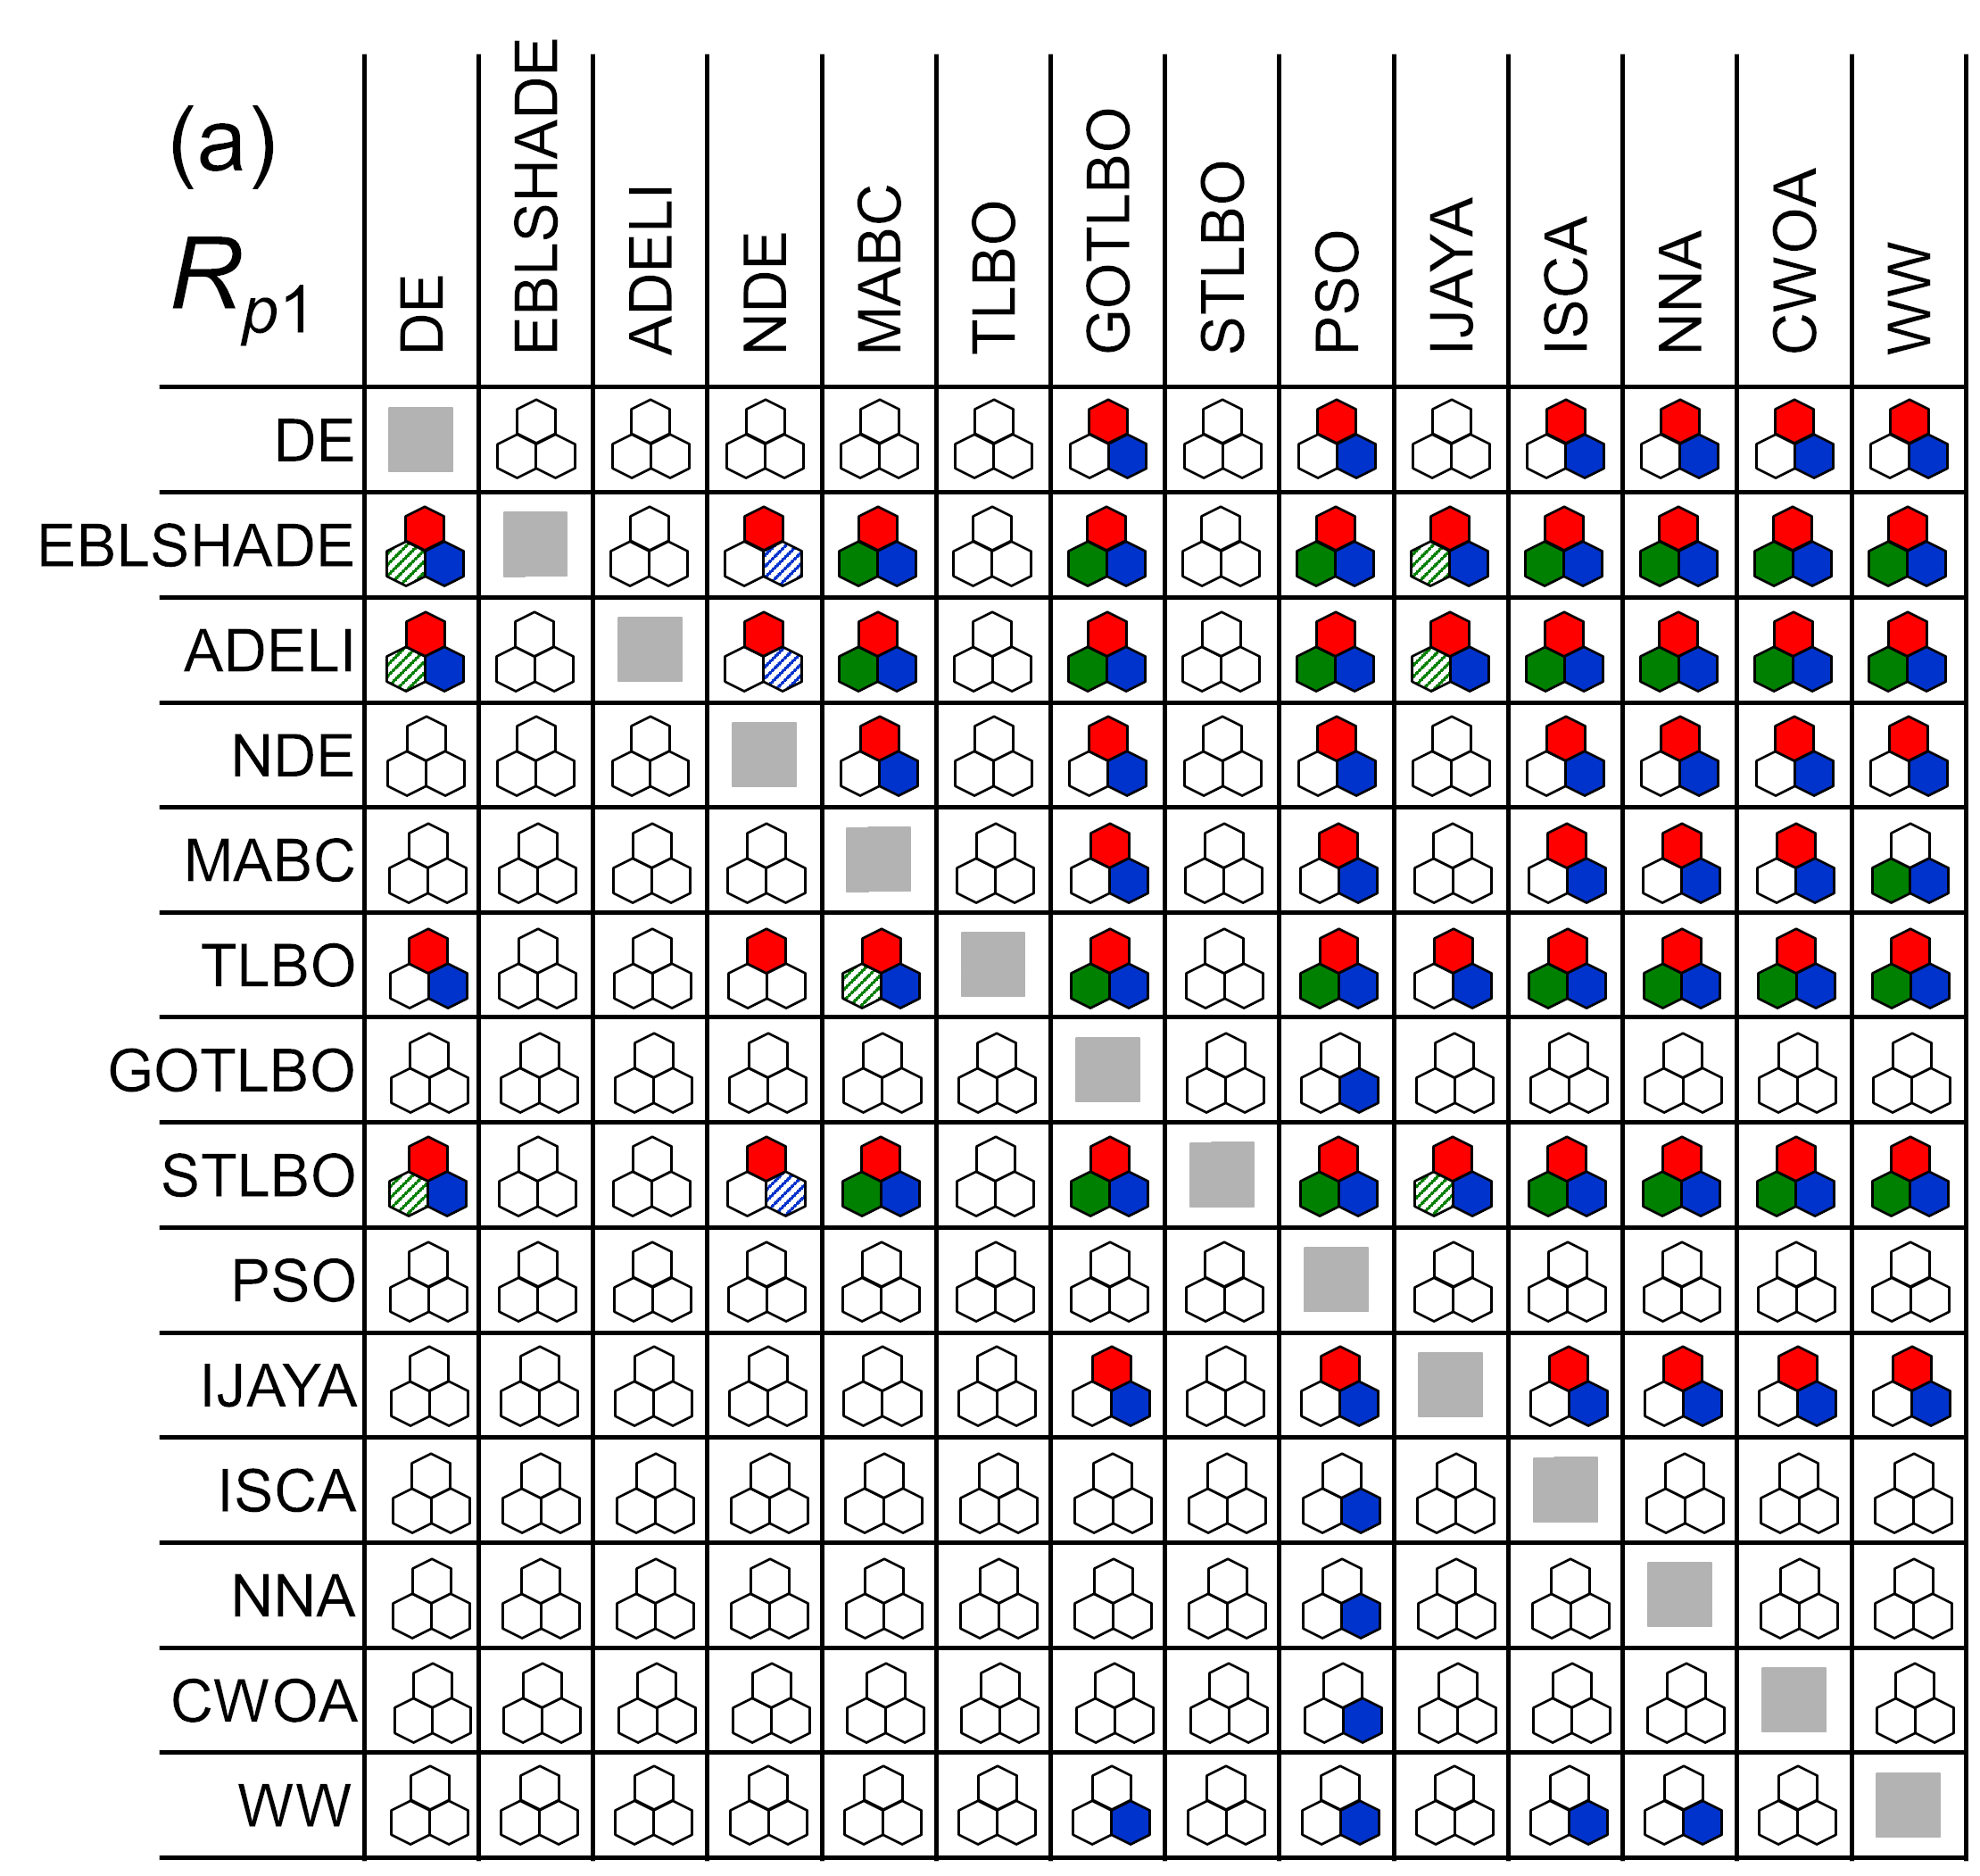
\includegraphics[width=.49\textwidth]{Rp1shotN1}
        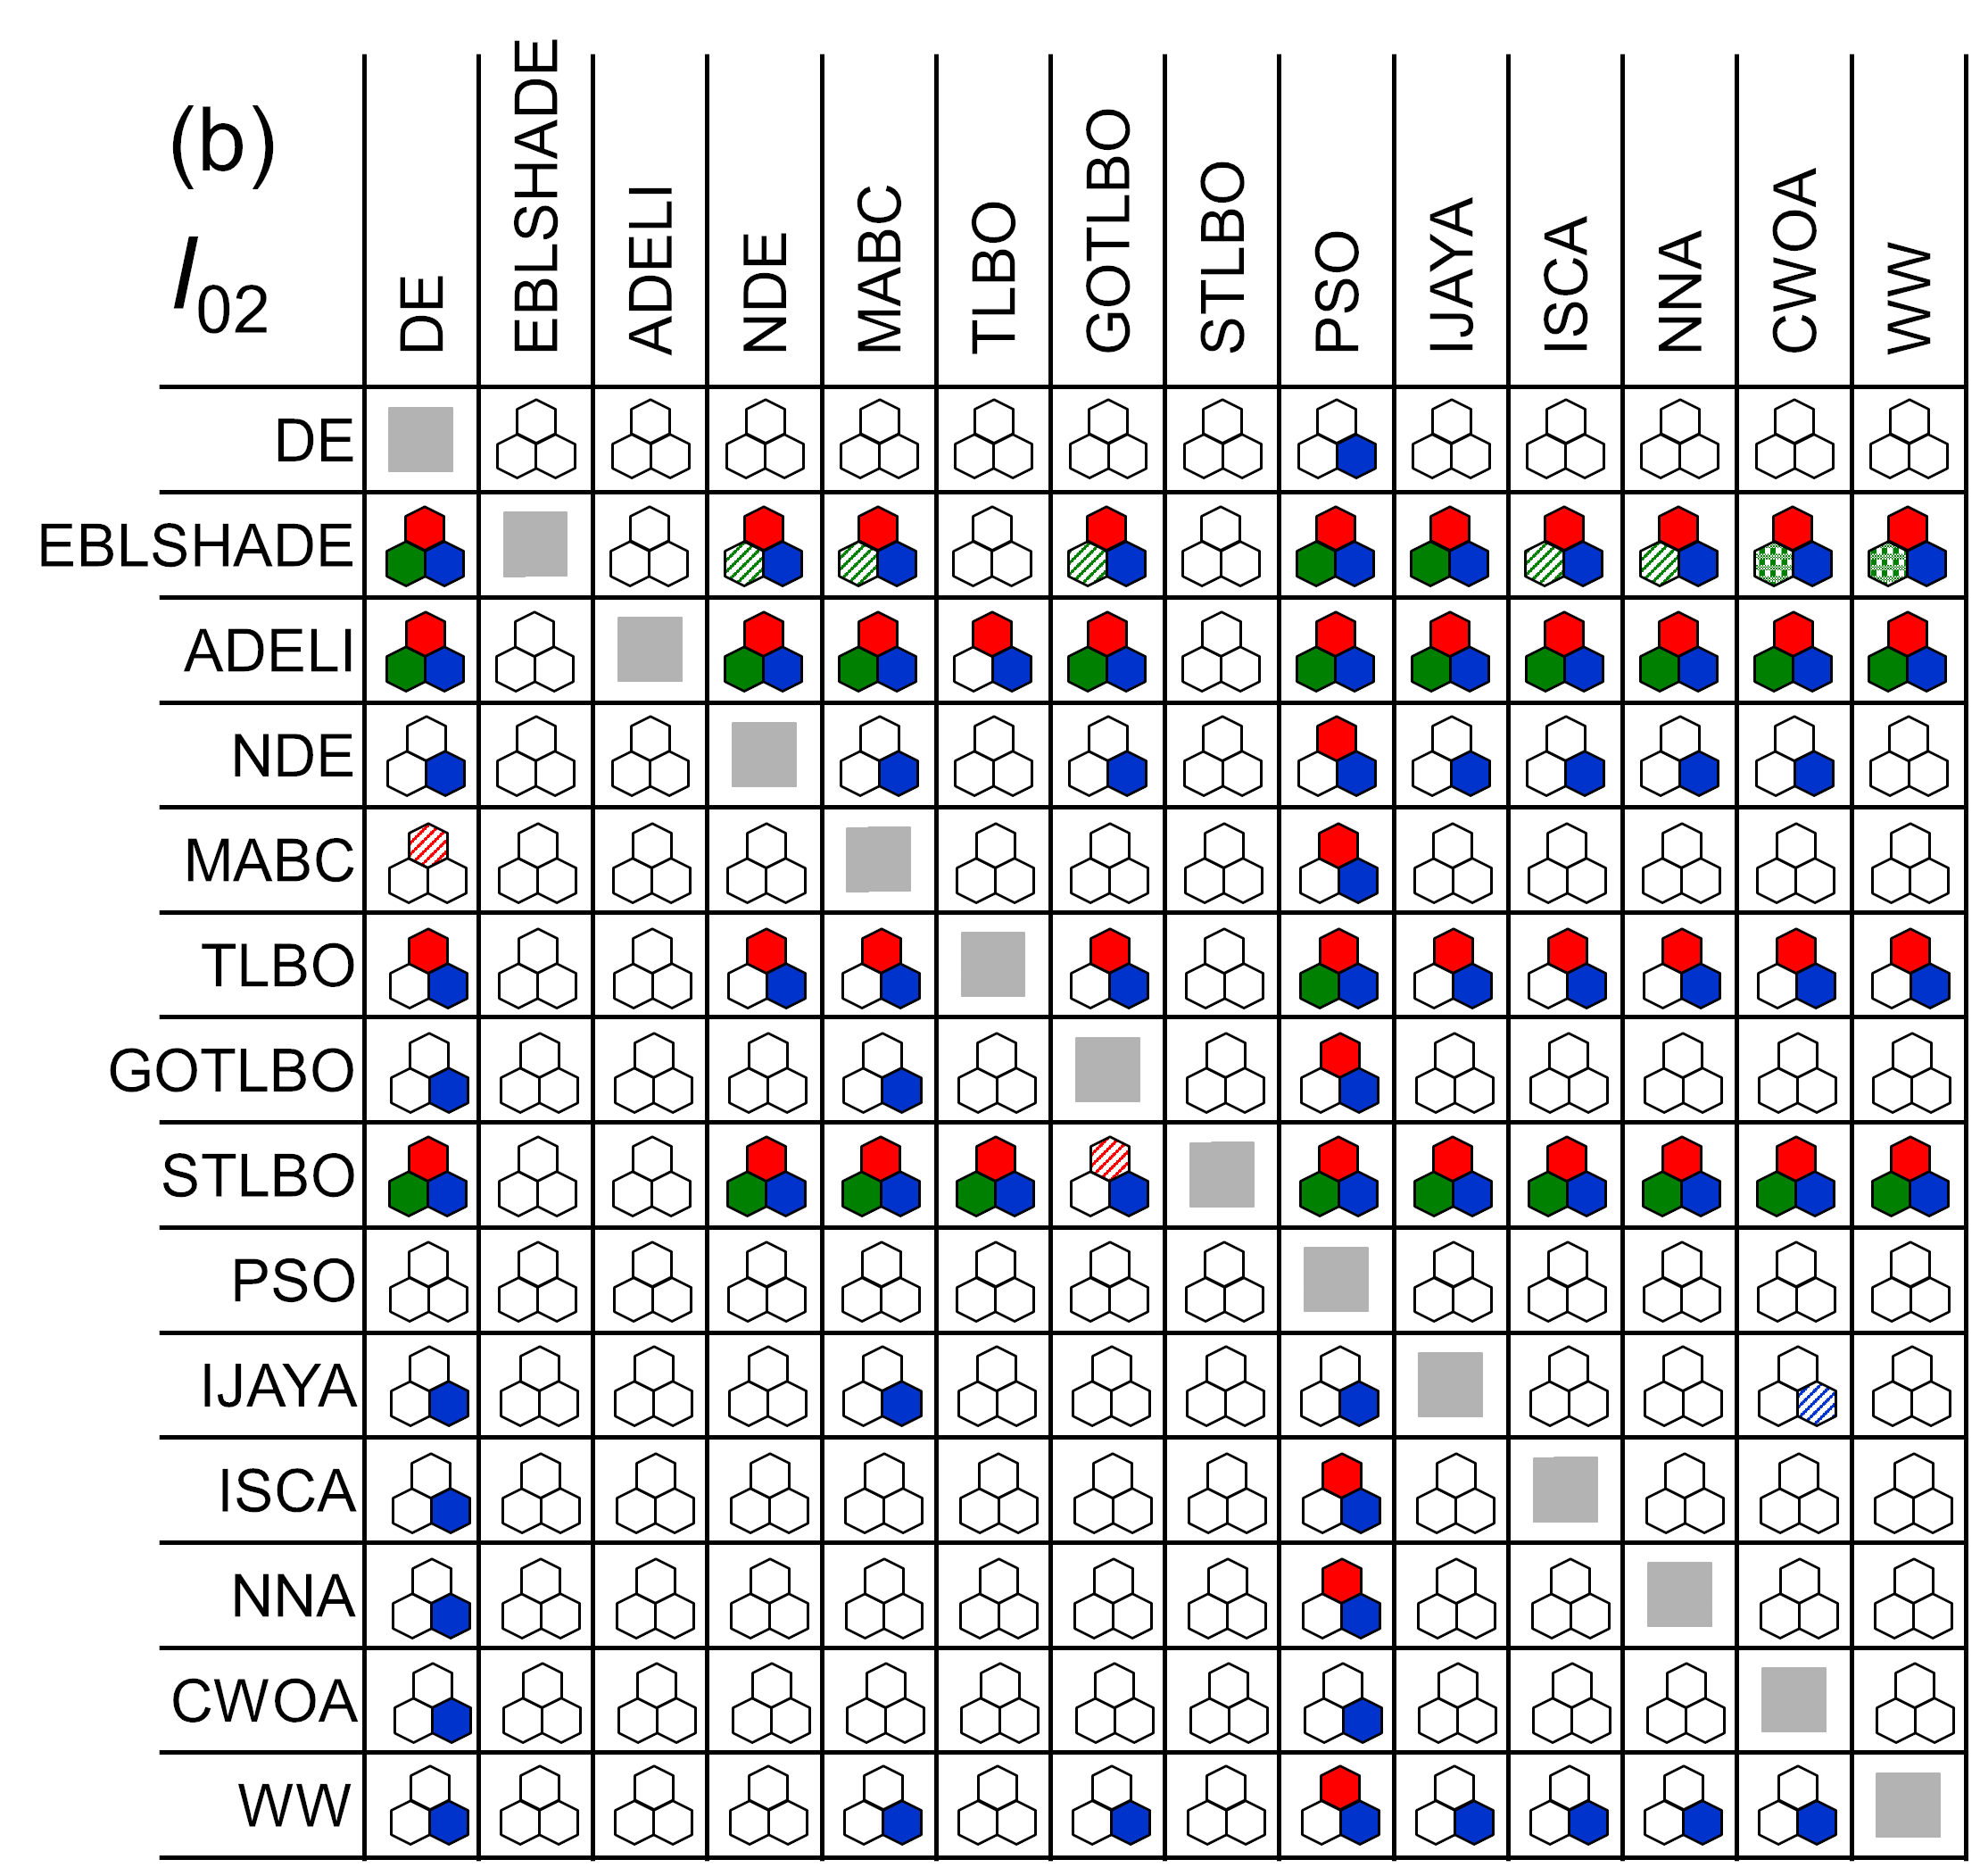
\includegraphics[width=.49\textwidth]{I02shotN1}
        
\includegraphics[width=.48\textwidth]{Titleshot11N}
		
\includegraphics[width=.48\textwidth]{Titleshot21N}
	  \caption{The results of algorithm $1\times N$ comparisons in $R_\mathrm{p1}$ (a) and $I_{02}$ (b) estimation
               by Friedman, Friedman Aligned, and Quade tests in the single--IV case.
               The colored hexagon indicates that the adjusted $p$-value,
               which tests the hypothesis that an algorithm in a row outperforms the algorithm in a column,
               is not greater than $p_{cr}=0.1$.
               The solid fill signifies that every post-hoc procedure resulted in $p<p_{cr}$;
               the patterned fill indicates that only specific post-hoc procedures achieved this outcome.
               The correspondence between the color and position of the hexagon to a test
               as well as the fill pattern to procedures are shown in a legend at the bottom of the figure.
               }\label{figN1RezSingleIV}
\end{figure*}


\begin{table*}[<options>]
\caption{The total count of wins and losses for each algorithm in $1\times N$ multiple comparisons using the
Friedman, Friedman Aligned, and Quade tests and Finner, Holm, Hochberg, and Holland post-hoc procedures
in single--IV case.
The criterion for victory was a adjusted $p$-value less than 0.1.
}\label{tbl1NWins}
\begin{tabular*}{\tblwidth}{@{}LCCCCCCCCCCC@{}}
\toprule
\multirow{3}{*}{Algorithm}& \multicolumn{11}{C}{Wins / Loses} \\
&  \multicolumn{10}{C}{task}  &\multirow{2}{*}{Total}\\
  & $I_{01}$& $n_1$ & $R_\mathrm{p1}$ &$I_{02}$& $n_2$& $R_\mathrm{p2}$&$R_\mathrm{s}$&$I_\mathrm{ph}$&RMSPE&Comp&\\ % Table header row
\midrule
DE & 24/43 & 56/34 & 48/35 &  4/73 & 48/43 & 49/34 & 49/40  & 45/35  & 49/48 & 16/27  & 388/412\\
EBLSHADE & 108/\textbf{0} & 108/\textbf{0}  & \textbf{107}/\textbf{0}  & 103/\textbf{0}  & 107/\textbf{0}  & 104/\textbf{0}  & 111/2  & \textbf{105}/\textbf{0}  &  \textbf{109}/\textbf{0}& \textbf{88}/\textbf{0}  & 1050/2 \\
ADELI & \textbf{122}/\textbf{0} & \textbf{110}/\textbf{0}  &  \textbf{107}/\textbf{0} &  \textbf{128}/\textbf{0} &  \textbf{110}/\textbf{0} &  \textbf{122}/\textbf{0} & \textbf{119}/\textbf{0}  & \textbf{105}/\textbf{0}  &  \textbf{109}/\textbf{0}& 61/2  & \textbf{1093}/2\\
NDE & 35/19  & 56/32  & 56/19  & 36/49  & 77/32  & 23/45  &  73/32 & 48/8 & 83/29 & 23/20  & 519/285\\
MABC &  8/61 & 28/69 & 44/45  &  9/57 & 40/55  & 4/82  & 32/51  & 32/66  & 44/62 & 8/30  & 249/578\\
TLBO & 80/3 & 102/\textbf{0} & 101/\textbf{0} &  84/13&  99/\textbf{0}& 87/18 & 93/10 & 94/\textbf{0} & 100/\textbf{0} & 65/2  & 905/46\\
GOTLBO & 8/60  & 12/73  & 4/84  & 16/49  & 20/74  & 13/54 & 20/61  & 4/80 & 16/85  & 13/28  & 126/648\\
STLBO & 109/\textbf{0} & \textbf{110}/\textbf{0}  & \textbf{107}/\textbf{0}  & 125/\textbf{0}  & 107/\textbf{0}  & 119/\textbf{0}  & 116/\textbf{0}  & \textbf{105}/\textbf{0}  & \textbf{109}/\textbf{0} & 81/\textbf{0}  & 1088/\textbf{0}\\
PSO & 0/84  & 8/88  & 0/100  & 0/108  & 4/101  & 0/96  &  0/124 & 0/96  & 20/70  & 4/49  & 72/916\\
IJAYA &  28/28 &  56/34 &  48/35 & 13/52  & 45/43 &  54/34 &  20/61 & 56/29  & 57/38  & 16/34  & 393/388\\
ISCA & 8/56  & 12/76  & 4/84  & 12/45  & 28/65  & 16/51  & 8/61  & 17/68  & 0/92  & 16/32  & 121/630\\
NNA & 33/29  & 0/92  & 4/84  & 12/49  & 12/84  & 12/57  & 8/77  & 12/80  & 0/92& 0/52  & 93/696\\
CWOA & 8/60  & 0/96  &  4/80& 8/52  & 8/84& 4/83  & 20/61  & 0/88  & 0/92 & 0/52  & 52/748\\
WW & 0/96  & 12/76  & 16/76&  36/43 & 0/108 & 10/60 & 12/77  & 12/66  & 0/92& 0/52  & 98/844\\
\bottomrule
\end{tabular*}
\end{table*}


%\begin{table}[<options>]
%\caption{Wilcoxon signed ranks test results of fitness functions comparisons with a level of significance $\alpha = 0.05$}\label{tblFF}
%\begin{tabular*}{\tblwidth}{@{}LCCCCCCCCC@{}}
%\toprule
%\multirow{2}{*}{Algorithm}& \multicolumn{9}{C}{Parameter} \\
%  & $I_{01}$& $n_1$ & $R_\mathrm{p1}$ &$I_{02}$& $n_2$& $R_\mathrm{p2}$&$R_\mathrm{s}$&$I_\mathrm{ph}$&RMSPE\\ % Table header row
%\midrule
%DE & SE & SE & = &  = & SE & SE & =  & =  & = \\
%EBLSHADE & SE & =  & =  & =  & =  & =  & =  & =  &  AE \\
%ADELI & SE & =  &  = &  = &  = &  = & =  & =  &   AE\\
%NDE & =  & =  & =  & =  & =  & =  &  = & SE & SE \\
%MABC &  = & SE & =  &  = & =  & =  & =  & =  & SE \\
%TLBO & SE & SE & SE &  SE&  SE& SE & SE & SE & SE \\
%GOTLBO & =  & =  & =  & =  & =  & SE & =  & =  & =  \\
%STLBO & SE & =  & =  & =  & =  & =  & =  & =  &  AE \\
%PSO & =  & =  & =  & =  & =  & =  &  AE & =  & =  \\
%IJAYA &  AE &  AE &  = & =  & SE &  = &  = & =  & =  \\
%ISCA & =  & =  & =  & =  & =  & =  & =  & =  & =  \\
%NNA & =  & =  & =  & =  & =  & =  & =  & =  &  SE\\
%CWOA & =  & =  &  SE& =  &   AE& =  & =  & =  & SE \\
%WW & =  & =  &  SE&  = &  AE &  = & =  & =  &  SE\\
%\bottomrule
%\end{tabular*}
%\end{table}


The statistical results of the algorithm's effectiveness comparison in the task  of $R_\mathrm{p1}$ estimation are shown in Fig.~\ref{figN1RezSingleIV}(a).
In the figure, the outperforming of an algorithm in a row over the algorithm in the column is indicated by a colored hexagon in the corresponding cell.
The white hexagon suggests a strong likelihood of the null hypothesis.
In fact, the data in Table~\ref{tbl1NADELI} were used to create the third row in Fig.~\ref{figN1RezSingleIV}(a).
The panel (b) of figure presents the statistical results for $I_{02}$ estimation.
The results of the comparison of algorithms based on the other eight parameters are given in the supplementary materials (figure S2).


The results displayed in Fig.~\ref{figN1RezSingleIV} demonstrate a consistent trend across all parameters.
Among the compared algorithms, EBLSHADE, ADELI, and STLBO consistently outperform the others in $1\times N$ multiple comparisons.
On the other hand, algorithms such as PSO, ISCA, CWOA, and NNA consistently produce lower-quality results.
The main changes observed in nonparametric statistical estimation of different parameters estimation
mainly concern algorithms with moderate effectiveness.

For example, when comparing the accuracy of determining $R_\mathrm{p1}$ and $I_{02}$,
the IJAYA algorithm performs better in the former case.
As evident from Figure 3a,
IJAYA outperforms GOTLBO, PSO, ISCA, NNA, CWOA, and WW in the results of Friedman
and Friedman Aligned tests for every post-hoc procedure considered.
While for $I_{02}$, IJAYA only outperforms DE, MABC, PSO, and CWOA according to the Friedman test,
and in the latter case, only for Finner post-hoc procedure.
For DE, the situation is similar in the case of $I_{02}$ compared to $R_\mathrm{p1}$.
According to the results of the Friedman and Friedman Aligned tests, the algorithm loses its advantage over GOTLBO, SCA, NNA, CWOA, and WW.
Additionally, the Friedman test no longer shows the improvement of DE over PSO.




In all cases, the Quade test yields higher adjusted $p$-values.
In particular, in the case of the complex parameter, none of the conducted comparisons exceeded the chosen threshold value of the $p$-value.

The adjusted $p$-values obtained from the direct comparisons of EBLSHADE, ADELI, and STLBO
do not allow for determining the best algorithm among them.
However, for this purpose, the results of this top trio of algorithms can be used,
obtained from their comparisons with less efficient optimization methods.
Table~\ref{tbl1NWins} summarizes count of wins and losses for each algorithm in $1\times N$ multiple comparisons.
The maximum possible number of wins achieved in every 10 tasks is 156,
obtained from comparing with 13 algorithms in 3 tests using 4 procedures.
As can be seen, among the compared algorithms,
ADELI showed the highest count of statistically confirmed improvements (1093) over others,
indicating its superior performance.
Conversely, STLBO demonstrated the lowest count of defeats (0) in similar comparisons, suggesting its consistently strong performance.

Previously, we employed procedures that controlled the Family-Wise Error Rate (FWER)
for comparisons with a control algorithm.
We tested each of the 14 algorithms individually to determine if any of them were superior to the others.
Below are the results of the carried out a multiple comparisons in which
all possible pairwise comparisons need to be computed ( $N\times N$ comparison),
and three procedures (Shaffer’s static, Nemenyi, and Holm) have been used to control FWER.
These procedures take into account that the hypotheses being tested belonging
to a family of all pairwise comparisons are logically interrelated;
thus not all combinations of true and false hypotheses are possible.

Starting from the analysis performed by the Friedman test over our results, we can raise the
91 hypotheses of equality among the 14 algorithms of our study for each task,
and apply the methods mentioned earlier to contrast them.
Table~\ref{tblNNpValueI01} lists the part of the hypotheses
and the adjusted $p$-values achieved on the task of $I_{01}$ estimation.
For the remaining 46 hypotheses not indicated in the table,
a $p$-value of 1 was obtained after applying each of the procedures.
The full version of the table as well as the data, obtained for other task,
are given in the supplementary material (tables~S144-S153).

\begin{table*}[<options>]
\caption{Adjusted $p$-values for tests for $N\times N$ multiple comparisons of $I_{01}$ estimation
         among all methods in the single--IV case ($p<1.0$ are only shown).}\label{tblNNpValueI01}
\begin{tabular*}{\tblwidth}{@{}LCCC@{}}
\toprule
\multirow{2}{*}{Hypothesis}& \multicolumn{3}{C}{post-hoc procedure} \\
  &Nemenyi & Holm & Shaffer\\ % Table header row
\midrule
ADELI versus WW&<1E-13&<1E-13&<1E-13\\
ADELI versus NDE&1.17195E-12&1.15907E-12&1.00453E-12\\
STLBO versus CWOA&1.17195E-12&1.15907E-12&1.00453E-12\\
TLBO versus PSO&1.21236E-12&1.17240E-12&1.03917E-12\\
STLBO versus GOTLBO&1.21236E-12&1.17240E-12&1.03917E-12\\
ADELI versus DE&1.73772E-12&1.64224E-12&1.48948E-12\\
STLBO versus DE&1.83875E-12&1.71752E-12&1.57607E-12\\
ADELI versus CWOA&3.83915E-12&3.50164E-12&3.29070E-12\\
EBLSHADE versus GOTLBO&4.20286E-12&3.78719E-12&3.60245E-12\\
STLBO versus NDE&5.01110E-12&4.46043E-12&4.29523E-12\\
ADELI versus GOTLBO&5.41522E-12&4.76064E-12&4.64162E-12\\
EBLSHADE versus CWOA&5.98099E-12&5.19229E-12&5.12657E-12\\
EBLSHADE versus ISCA&1.17195E-11&1.00453E-11&1.00453E-11\\
EBLSHADE versus DE&1.45282E-11&1.22931E-11&1.06966E-11\\
EBLSHADE versus NDE&4.17053E-11&3.43725E-11&3.07061E-11\\
STLBO versus ISCA&8.17133E-11&6.64482E-11&6.01625E-11\\
TLBO versus WW&8.82197E-11&7.07696E-11&6.49529E-11\\
TLBO versus MABC&1.07900E-10&8.53717E-11&7.94431E-11\\
EBLSHADE versus MABC&3.09961E-10&2.38431E-10&2.28213E-10\\
ADELI versus NNA&3.24570E-10&2.46102E-10&2.38969E-10\\
ADELI versus ISCA&3.83410E-10&2.86504E-10&2.82291E-10\\
STLBO versus MABC&1.58351E-09&1.16588E-09&1.16588E-09\\
STLBO versus NNA&1.83408E-09&1.33021E-09&1.33021E-09\\
TLBO versus ISCA&3.49326E-09&2.49519E-09&2.22648E-09\\
ADELI versus MABC&5.83612E-09&4.10452E-09&3.71972E-09\\
EBLSHADE versus NNA&1.23520E-08&8.55140E-09&7.87272E-09\\
EBLSHADE versus PSO&1.47150E-08&1.00256E-08&9.37877E-09\\
STLBO versus PSO&5.32586E-08&3.57008E-08&3.39450E-08\\
ADELI versus PSO&1.50038E-07&9.89261E-08&.56286E-08\\
TLBO versus GOTLBO&2.16253E-07&1.40208E-07&1.37831E-07\\
EBLSHADE versus WW&2.39169E-07&1.52438E-07&1.52438E-07\\
TLBO versus CWOA&2.89034E-07&1.81043E-07&1.77867E-07\\
TLBO versus DE&5.91345E-07&3.63905E-07&3.63905E-07\\
STLBO versus WW&6.86296E-07&4.14794E-07&4.14794E-07\\
TLBO versus NDE&1.37158E-06&8.13904E-07&7.68687E-07\\
TLBO versus NNA&1.17758E-04&6.72904E-05&6.59964E-05\\
NNA versus WW&2.21281E-02&1.24015E-02&1.24015E-02\\
IJAYA versus WW&2.36193E-01&1.29777E-01&1.24585E-01\\
NNA versus PSO&2.36193E-01&1.29777E-01&1.24585E-01\\
NDE versus WW&4.04596E-01&2.13413E-01&2.13413E-01\\
DE versus WW&6.28685E-01&3.24706E-01&3.24706E-01\\
CWOA versus WW&8.94683E-01&4.52257E-01&4.52257E-01\\
GOTLBO versus WW&1.0&5.07626E-01&5.07626E-01\\
IJAYA versus PSO&1.0&8.15876E-01&7.97333E-01\\
NNA versus MABC&1.0&9.64793E-01&9.64793E-01\\
\bottomrule
\end{tabular*}
\end{table*}


It can be seen that using a level of significance 0.1, only 37 hypotheses of equality
are rejected by the Nemenyi, Holm, and Shaffer methods.
These hypotheses show the improvement of EBLSHADE, ADELI,  TLBO, and STLBO
over DE, NDE, MABC, GOTLBO, PSO, ISCA, NNA, CWOA, and WW,
and NNA over WW.
None of the remaining 54 hypotheses can be rejected using these procedures.

It should be noted that when testing complementary hypotheses
(``algorithm A vs algorithm B'' and ``algorithm B vs algorithm A''),
only in one out of the two cases can a $p$-value less than 1 be obtained.
For instance, when using the Nemenyi procedure to task $I_{01}$ evaluating of comparing ``ADELI vs MABC''
a $p$-value of $5.84\cdot10^{-9}$ was obtained.
Conversely, when comparing ``MABC vs ADELI'', the $p$-value was 1.
The $p$-values were computed for all possible hypotheses in the study to identify algorithms whose results statistically deviate from those of other algorithms.
In this case, a critical value of $p_{cr}=0.1$ was used, similar to the $1\times N$ multiple comparisons.
Typical examples of the obtained results for specific parameter cases are presented in Fig.~\ref{figNNRezSingleIV}.
For more comprehensive data, please refer to figure S3 in the supplementary materials.
Generalized results regarding the total count of victories and defeats in the $N\times N$ comparisons are listed in Table~\ref{tblNNWins}.
In the case of $N\times N$ comparisons, the maximum possible number of wins achieved in every 10 tasks is 39,
obtained from comparing 13 algorithms in 3 post-hoc procedures.

\begin{figure*}[!ht]
	\centering
		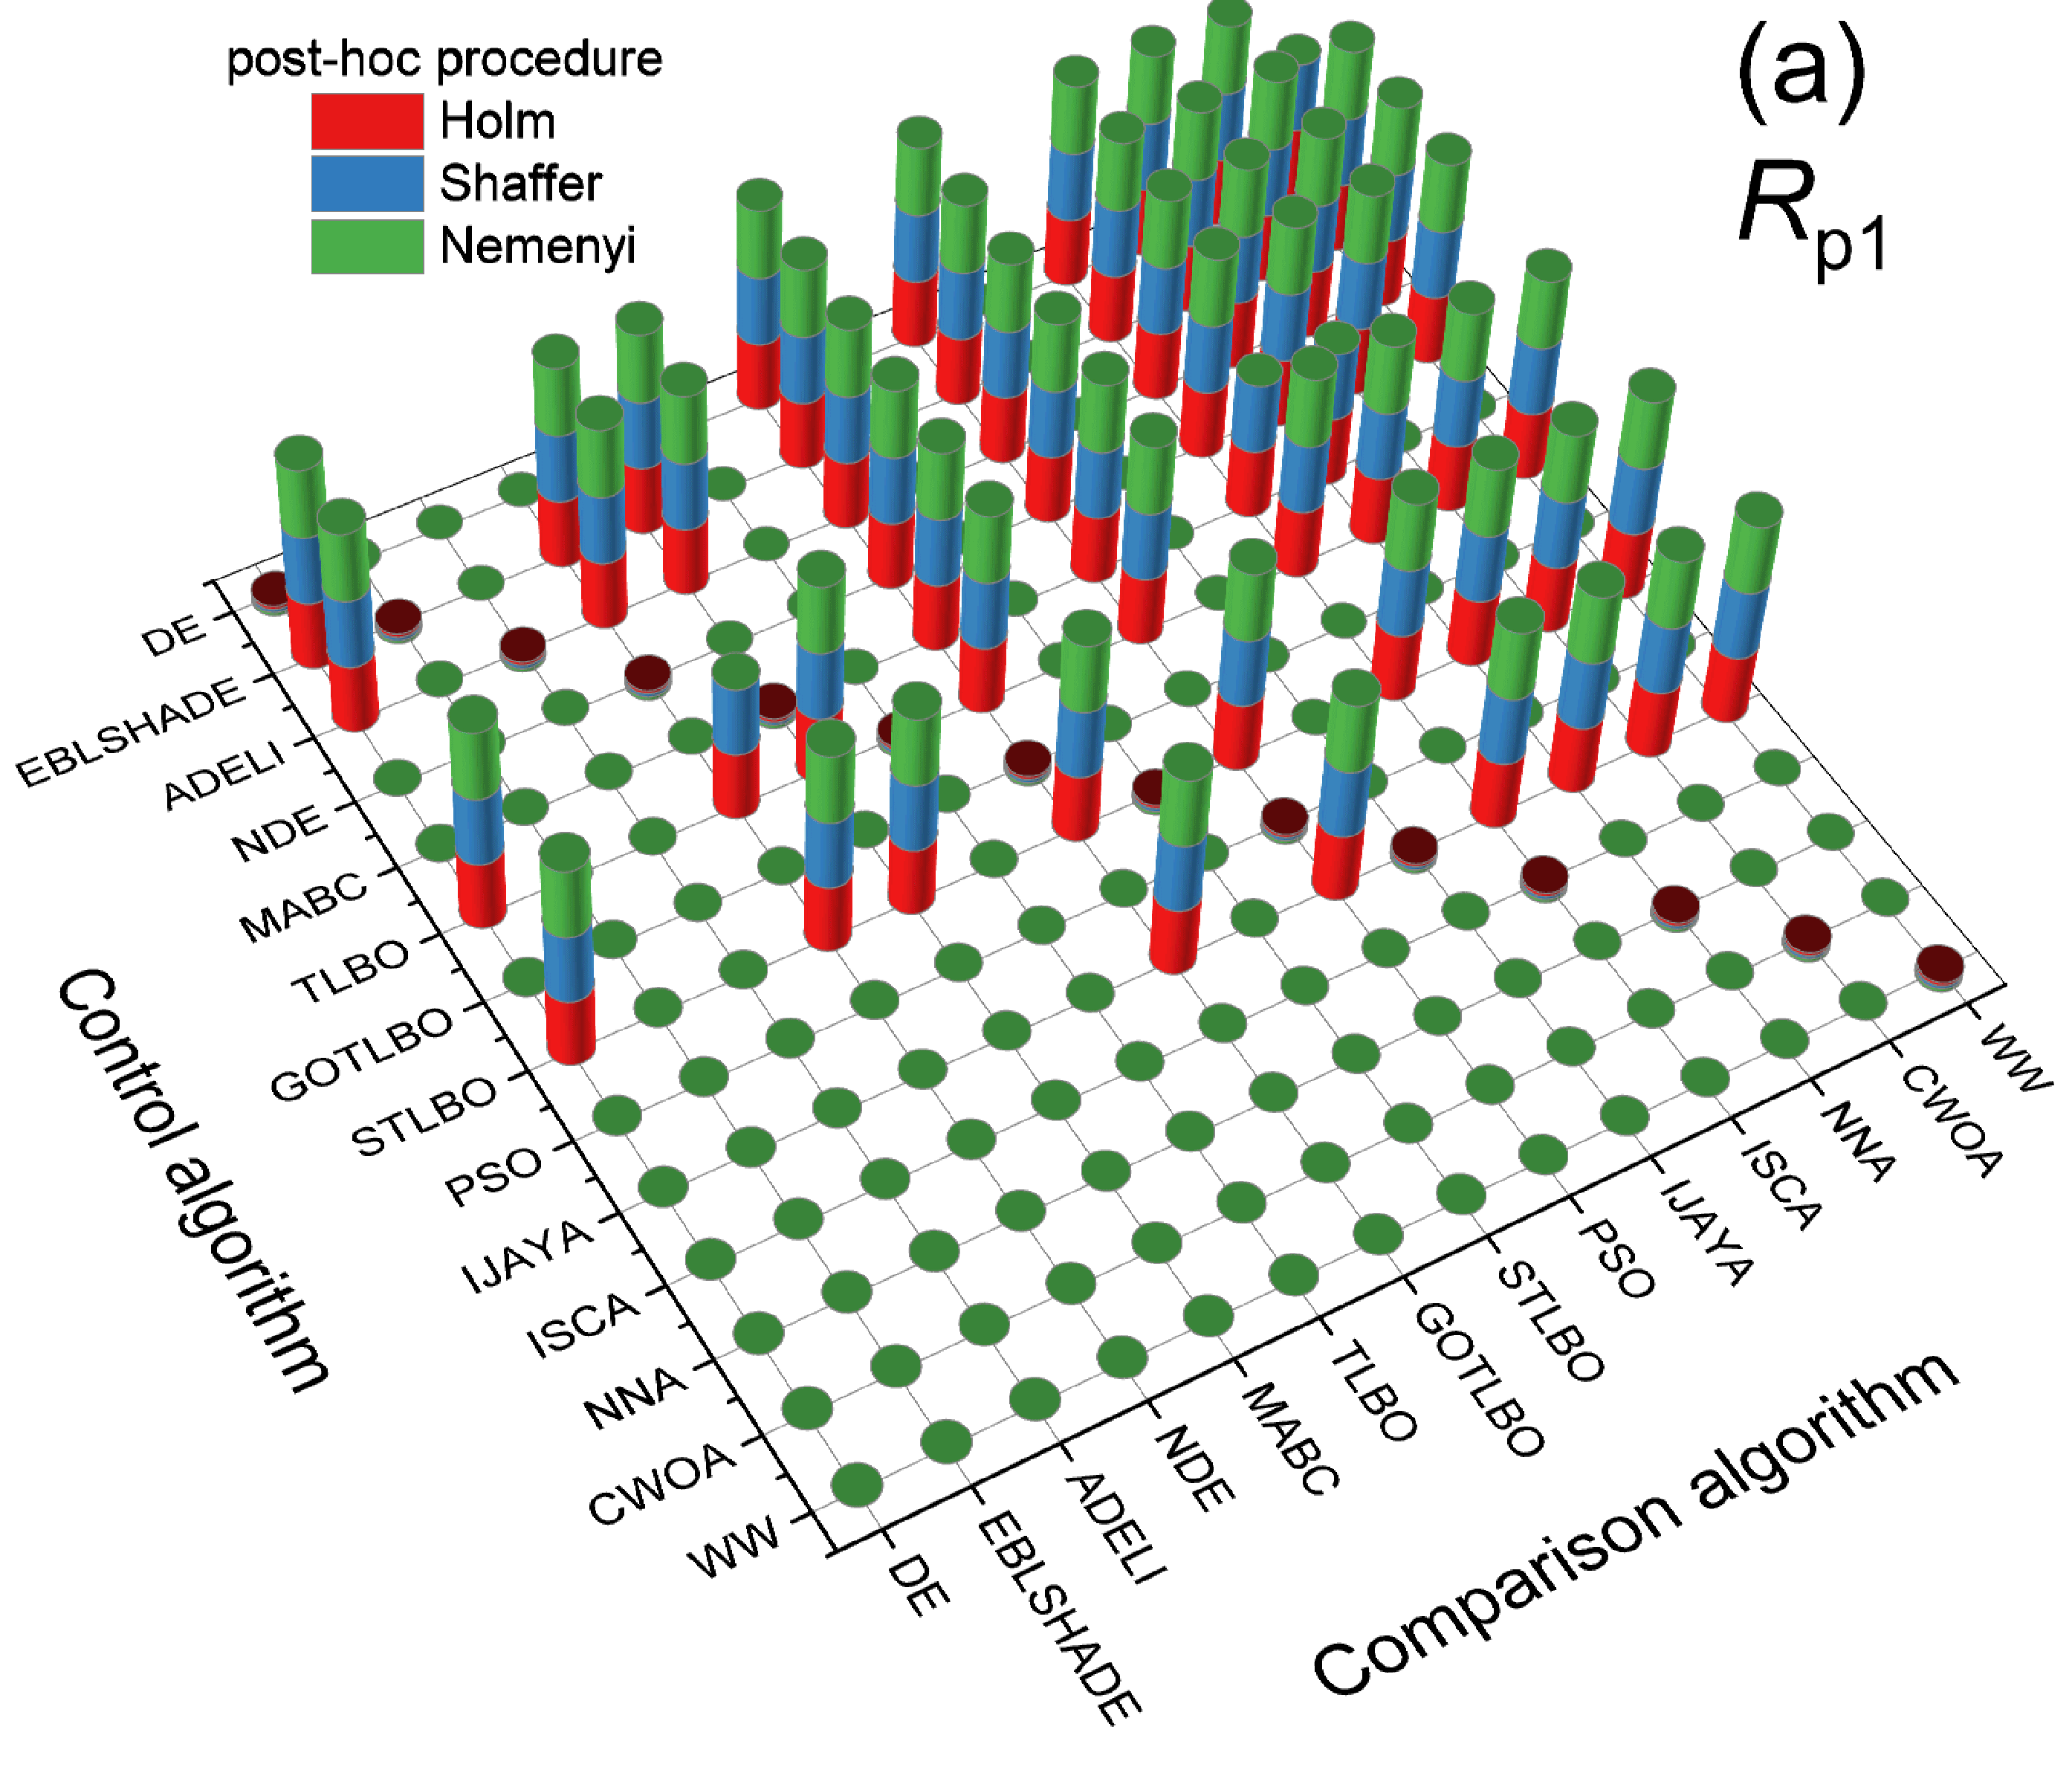
\includegraphics[width=.49\textwidth]{Rp1shot_NN}
        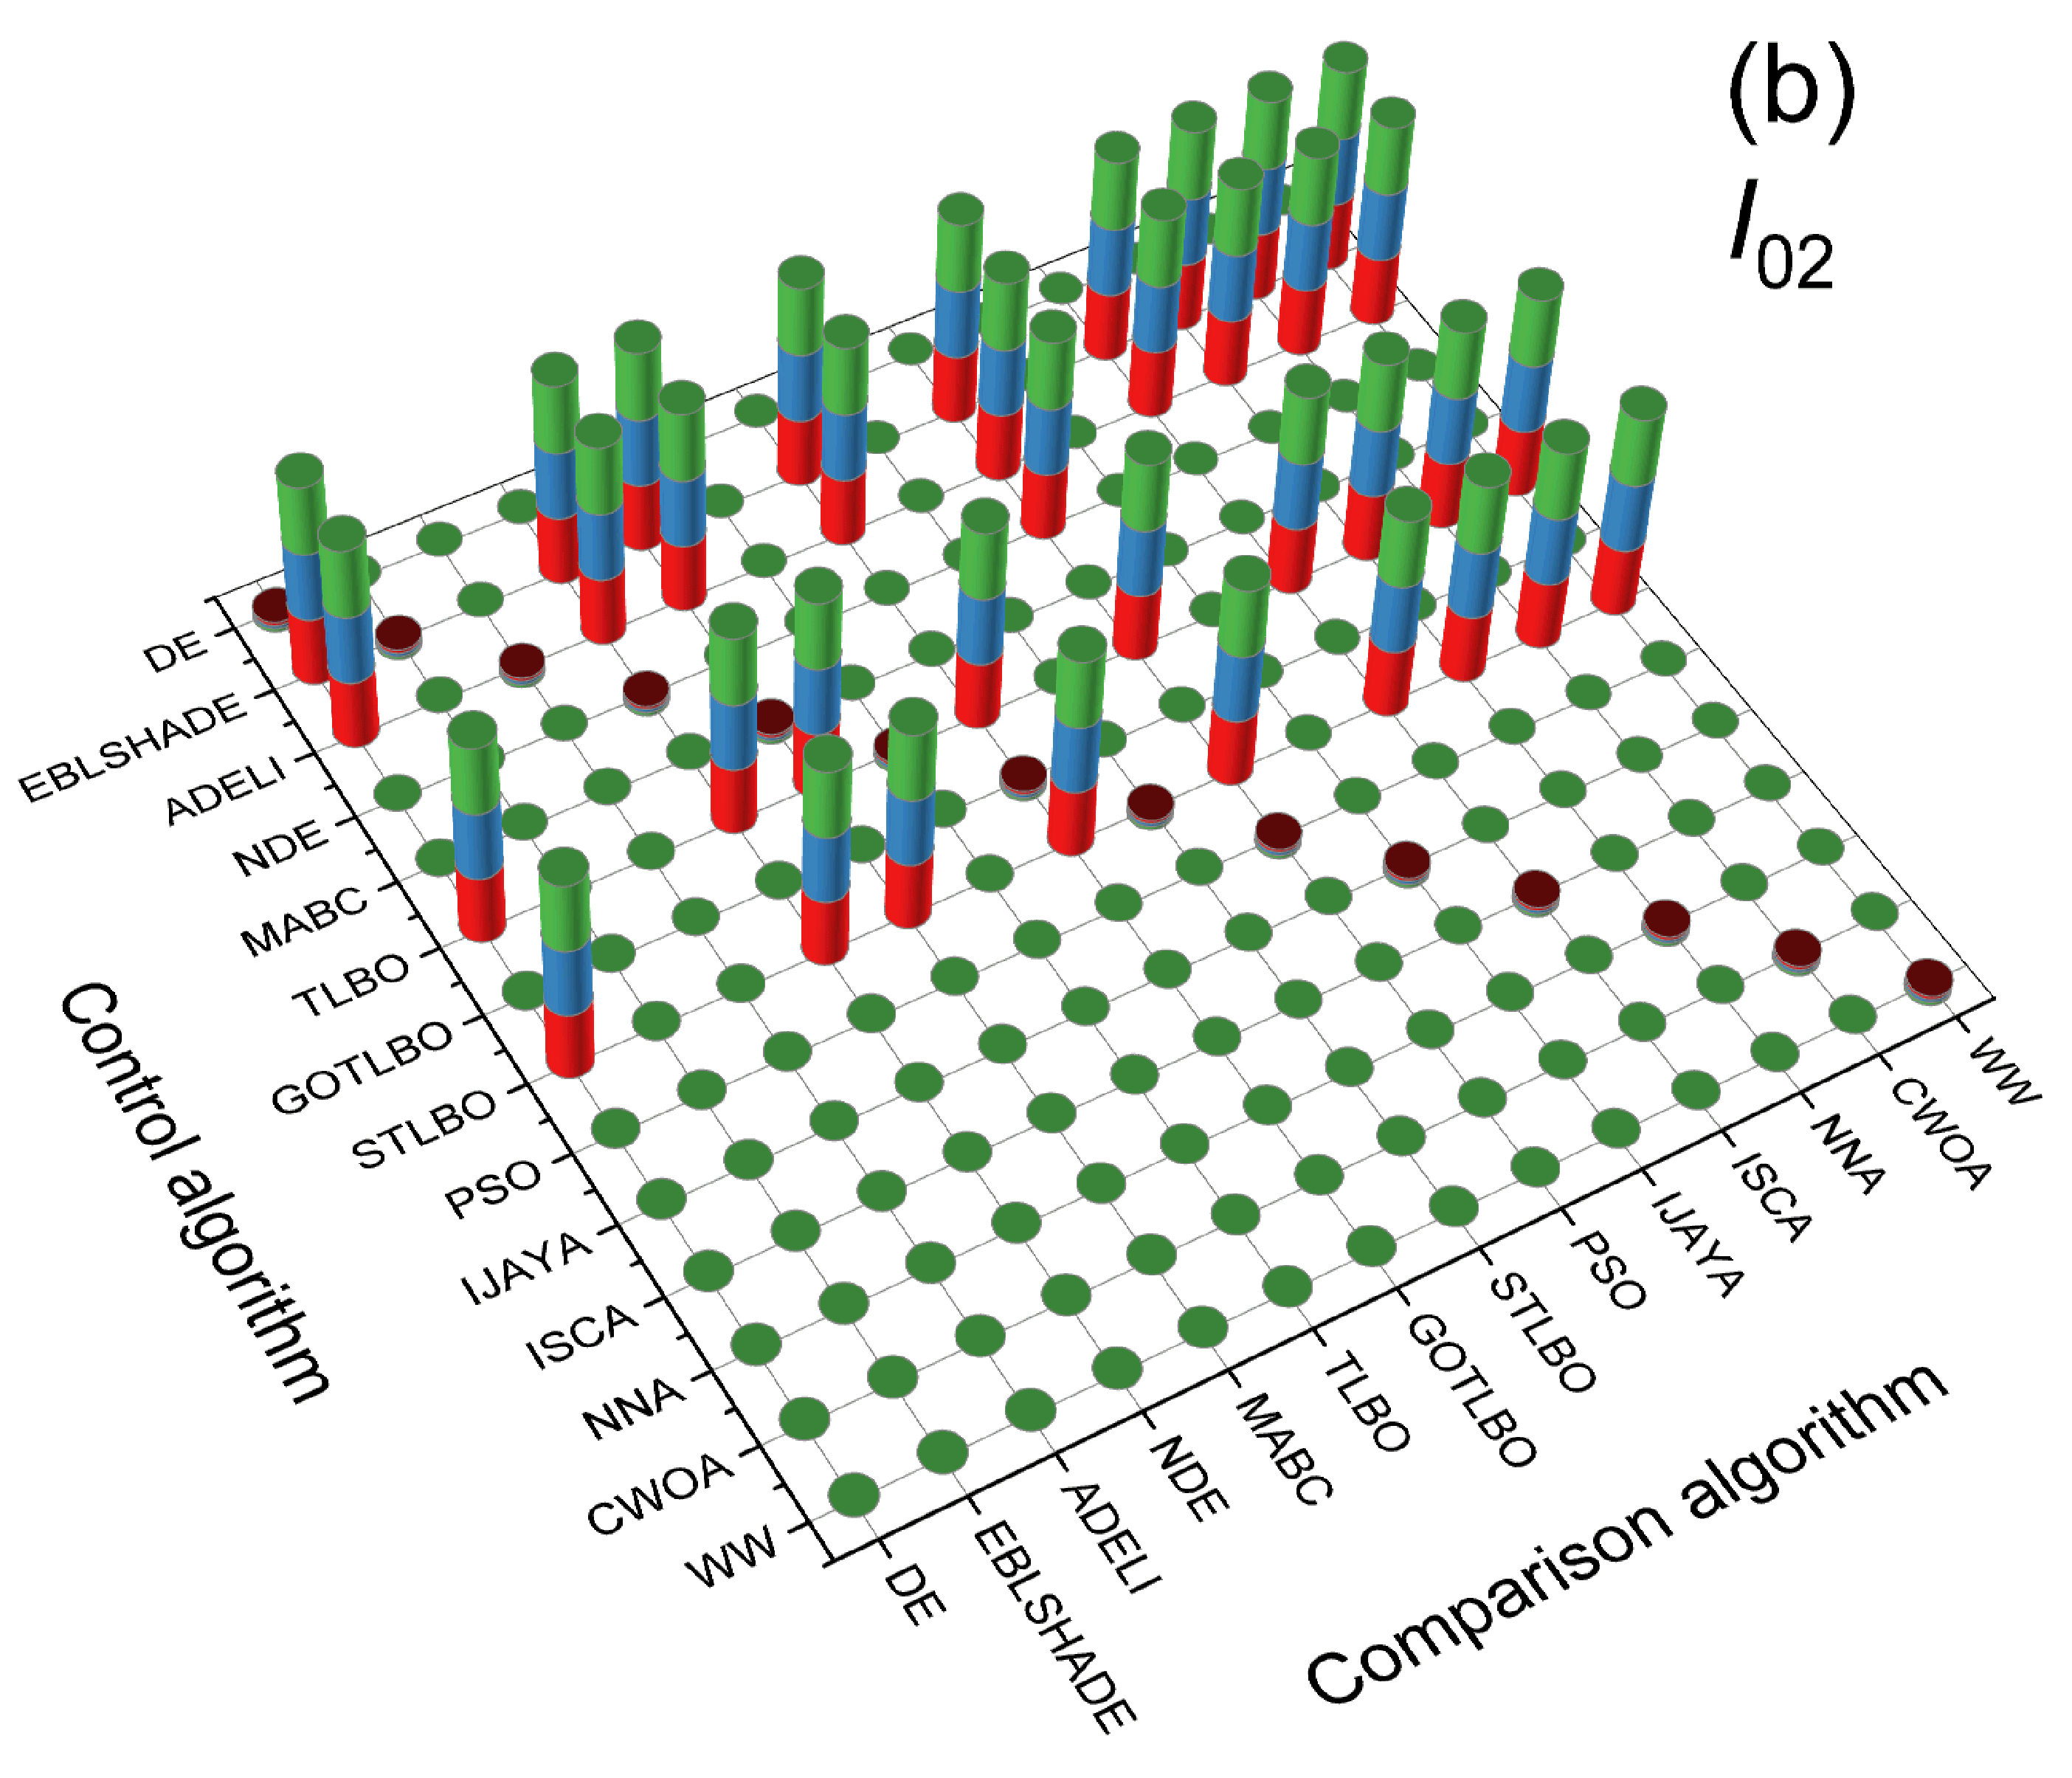
\includegraphics[width=.49\textwidth]{I02shot_NN}
	  \caption{The results of $N\times N$ multiple comparisons of $R_\mathrm{p1}$ (a) and $I_{02}$ (b) estimation
               among all algorithms in the single--IV case.
               The colored cylinder indicates that the adjusted $p$-value,
               which tests the control algorithm outperforms the comparison algorithm,
               is not greater than $p_{lim}=0.1$.
               The correspondence between the color of the cylinder to a post-hoc procedure is shown in the figure's legend.
               }\label{figNNRezSingleIV}
\end{figure*}

\begin{table*}[<options>]
\caption{The total count of wins and losses for each algorithm in $N\times N$ multiple comparisons using the
Friedman test and Shaffer's static, Nemenyi, and Holm post-hoc procedures
in single--IV case.
The criterion for victory was a adjusted $p$-value less than 0.1.
}\label{tblNNWins}
\begin{tabular*}{\tblwidth}{@{}LCCCCCCCCCCC@{}}
\toprule
\multirow{3}{*}{Algorithm}& \multicolumn{11}{C}{Wins / Loses} \\
&  \multicolumn{10}{C}{task}  &\multirow{2}{*}{Total}\\
  & $I_{01}$& $n_1$ & $R_\mathrm{p1}$ &$I_{02}$& $n_2$& $R_\mathrm{p2}$&$R_\mathrm{s}$&$I_\mathrm{ph}$&RMSPE&Comp&\\ % Table header row
\midrule
DE & 0/12 & 17/12 & 17/12 &  0/12 & 12/12 & 14/12 & 5/12  & 17/12  & 15/15 & 0/0  & 97/111\\
EBLSHADE & 27/0 & 27/0  & 27/0  & 27/0  & 27/0  & 27/0  & 27/0 & 27/0  &  26/0& 21/0  & \textbf{263}/\textbf{0} \\
ADELI & 27/0 & 27/0  &  27/0 &  27/0 &  27/0 &  27/0 & 27/0  & 27/0  &  27/0& 14/0  & 257/\textbf{0}\\
NDE & 0/12  & 21/12  & 18/11  & 3/12  & 18/9  & 3/12  &  18/11 & 21/9 & 24/8 & 0/0  & 126/96\\
MABC &  0/12& 0/15& 10/12  &  0/12 & 11/12  & 0/17  & 3/12  & 2/15  & 12/15 & 0/3  & 38/125\\
TLBO & 27/0& 27/0 & 26/0 &  27/0&  24/0& 27/0 & 26/0 & 24/0 & 24/0 & 10/0  & 242/0\\
GOTLBO & 0/12  & 0/18  & 0/24  & 0/12  & 3/15  & 0/12 & 3/15  & 0/21 & 0/21  & 0/5  & 6/155\\
STLBO & 27/0 & 27/0  & 27/0  & 27/0  & 27/0  & 27/0  & 27/0  & 27/0  & 27/0 & 11/0  & 254/\textbf{0}\\
PSO & 0/12  & 0/21  & 0/24  & 0/15  & 0/24  & 0/21  &  0/34 & 0/23  & 0/18  & 0/12  & 0/204\\
IJAYA &  0/0 &  16/0 &  18/0 & 0/0  & 12/0 &  11/0 &  3/0 & 18/0  & 18/0  & 0/0  & 96/\textbf{0}\\
ISCA & 0/12  & 0/21  & 0/23  & 0/12  & 3/15  & 0/12  & 2/15  & 0/21  & 0/24 & 0/3  & 5/158\\
NNA & 3/12  & 0/21  & 0/23  & 0/12  & 0/23  & 0/14  & 0/17  & 0/21  & 0/24& 0/9  & 3/176\\
CWOA & 0/12  & 0/21  &  0/21& 0/12  & 0/24& 0/18  & 3/15  & 0/21  & 0/24 & 0/12  & 3/180\\
WW & 0/15  & 0/21  & 0/20&  0/12 & 0/30 & 0/18 & 2/15  & 0/20  & 0/24& 0/12  & 2/187\\
\bottomrule
\end{tabular*}
\end{table*}


In the majority of cases, all post-hoc procedures considered lead to similar conclusions regarding the outperforming of one algorithm over another.
For example, in the case of the $R_\mathrm{p1}$ estimation task,
the Nemenyi procedure disagrees with Holm and Shaffer methods in only 4 out of 57 cases.
Specifically, this occurs for the hypotheses "DE vs WW," "MABC vs ISCA," "MABC vs NNA," and "TLBO vs NDE" --- see Fig.~\ref{figNNRezSingleIV}(a).
On the other hand, as evident from Fig.~\ref{figNNRezSingleIV}(b), such situations are not observed at all for the $I_{02}$ task.
The Holm procedure results, in general, differs from the Shaffer procedure ones in only two comparisons:
the improvement of IJAYA over GOTLBO in the $n_1$ estimation and the outperforming of TLBO over NNA for the composite parameter.

Totally $1\times N$ multiple comparisons exhibit more powerful behavior than $N\times N$ ones, reaching the lower $p$-values.
As a result, IJAYA did not lose in any of the $N\times N$ comparisons --- see Table~\ref{tblNNWins}.
Another striking  example can be observed when considering the case of the composite parameter.
Based on the $1\times N$ comparisons, conclusions were drawn about the outperforming of one algorithm over another in 67 cases,
whereas for the $N\times N$ comparisons, such situations were found in only 20 cases:
the improvement of EBLSHADE over MABC, GOTLBO, PSO, ISCA, NNA, CWOA, and WW,
the statistically significant difference ADELI and GOTLBO, PSO, NNA, CWOA, and WW,
and outperforming of both TLBO and STLBO over PSO, NNA, CWOA, and WW.
Consequently, $N\times N$ comparisons provide a less precise ranking of all algorithms.
However, it is still possible to identify the best and worst-performing algorithms.
The obtained data reveal that EBLSHADE, ADELI, and STLBO are the top-performing algorithms in all tasks,
while PSO, ISCA, NNA, CWOA, and WW are the worst-performing.

Thus, the results presented in this subsection demonstrate that
among the examined algorithms, none can be applied for the maximally accurate determination
of a specific individual parameter (e.g., only $R_\mathrm{p2}$ or only $I_{02}$) in the opposed two-diode model.
The algorithms that exhibit high efficiency (EBLSHADE, ADELI, and STLBO) allow for the most precise estimation of all parameters.
However, certain algorithms really display higher accuracy in determining specific parameters.
Indeed, DE and IJAYA are the most effective in estimating $R_\mathrm{p2}$ and $I_\mathrm{ph}$ --- see table~S1.
Nevertheless, this highest level of accuracy appears unworthy of significant attention when compared to other optimization methods.
As a result, the performance metrics of algorithms for individual parameters will not be analyzed
in the following subsection, dedicated to the analysis of IV curves with different parameter ratios.




\subsubsection{Evaluation of IV--set}


\begin{figure*}[]
	\centering
		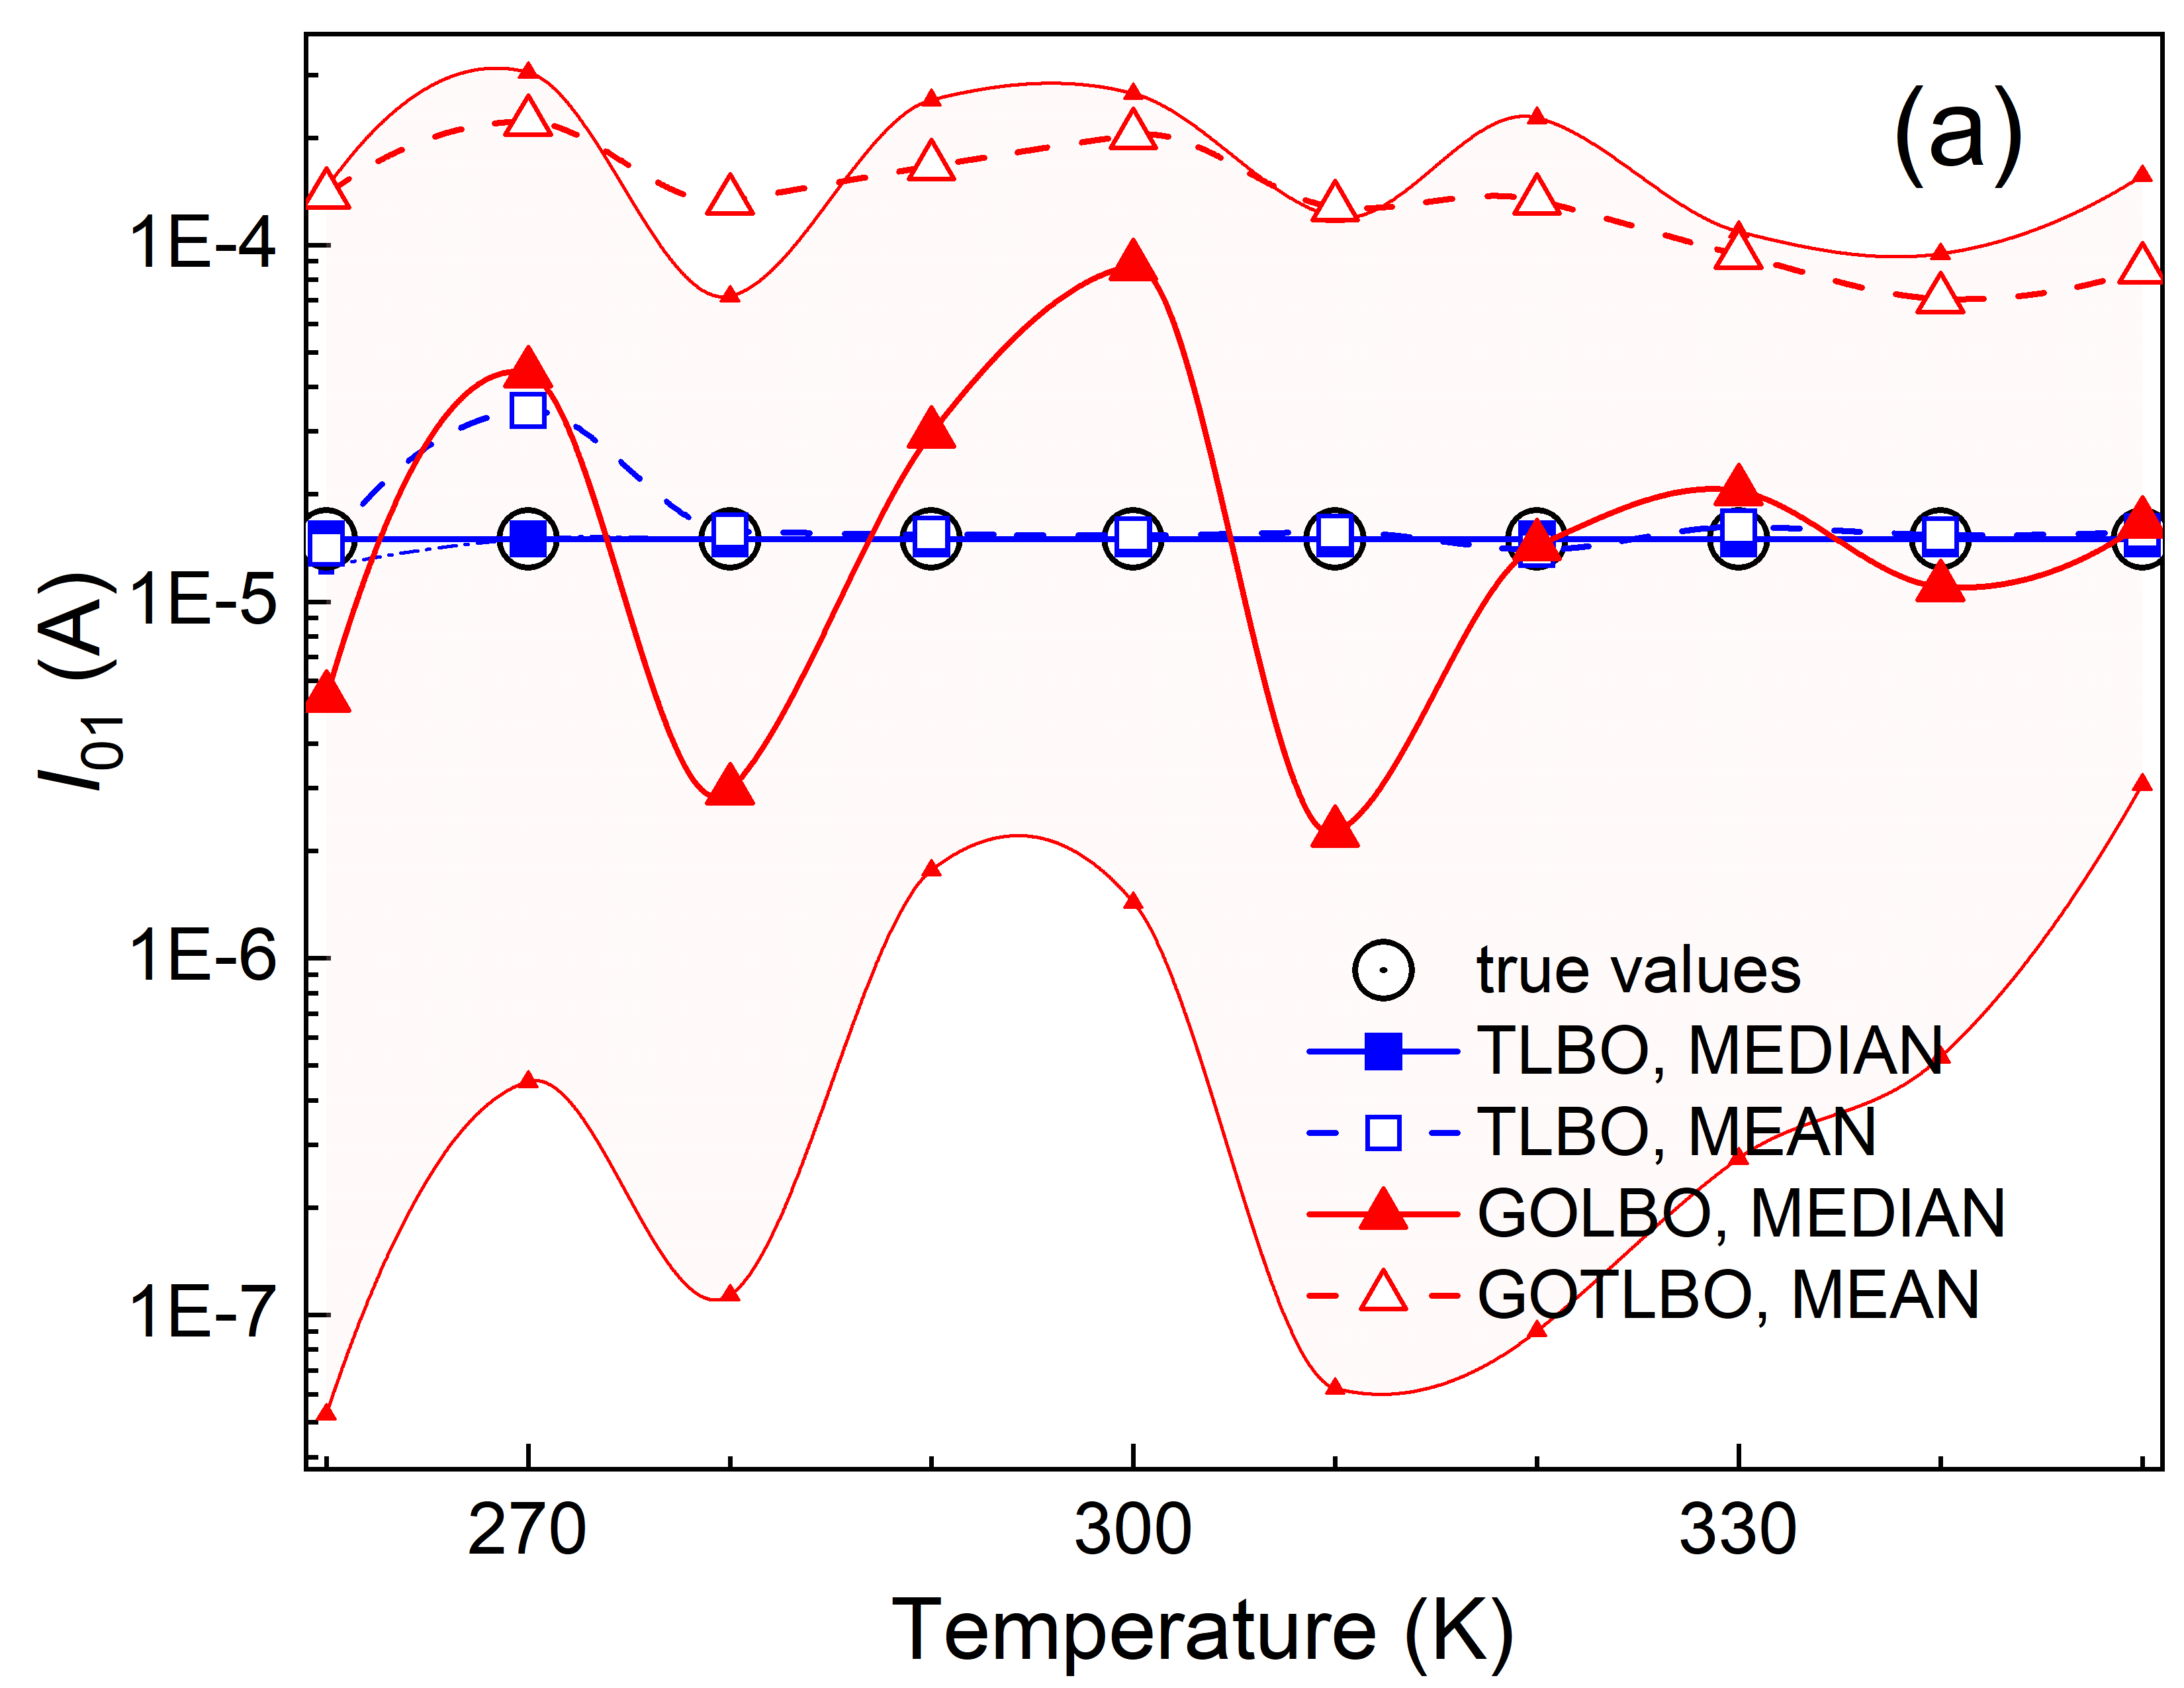
\includegraphics[width=.32\textwidth]{AfigA}
        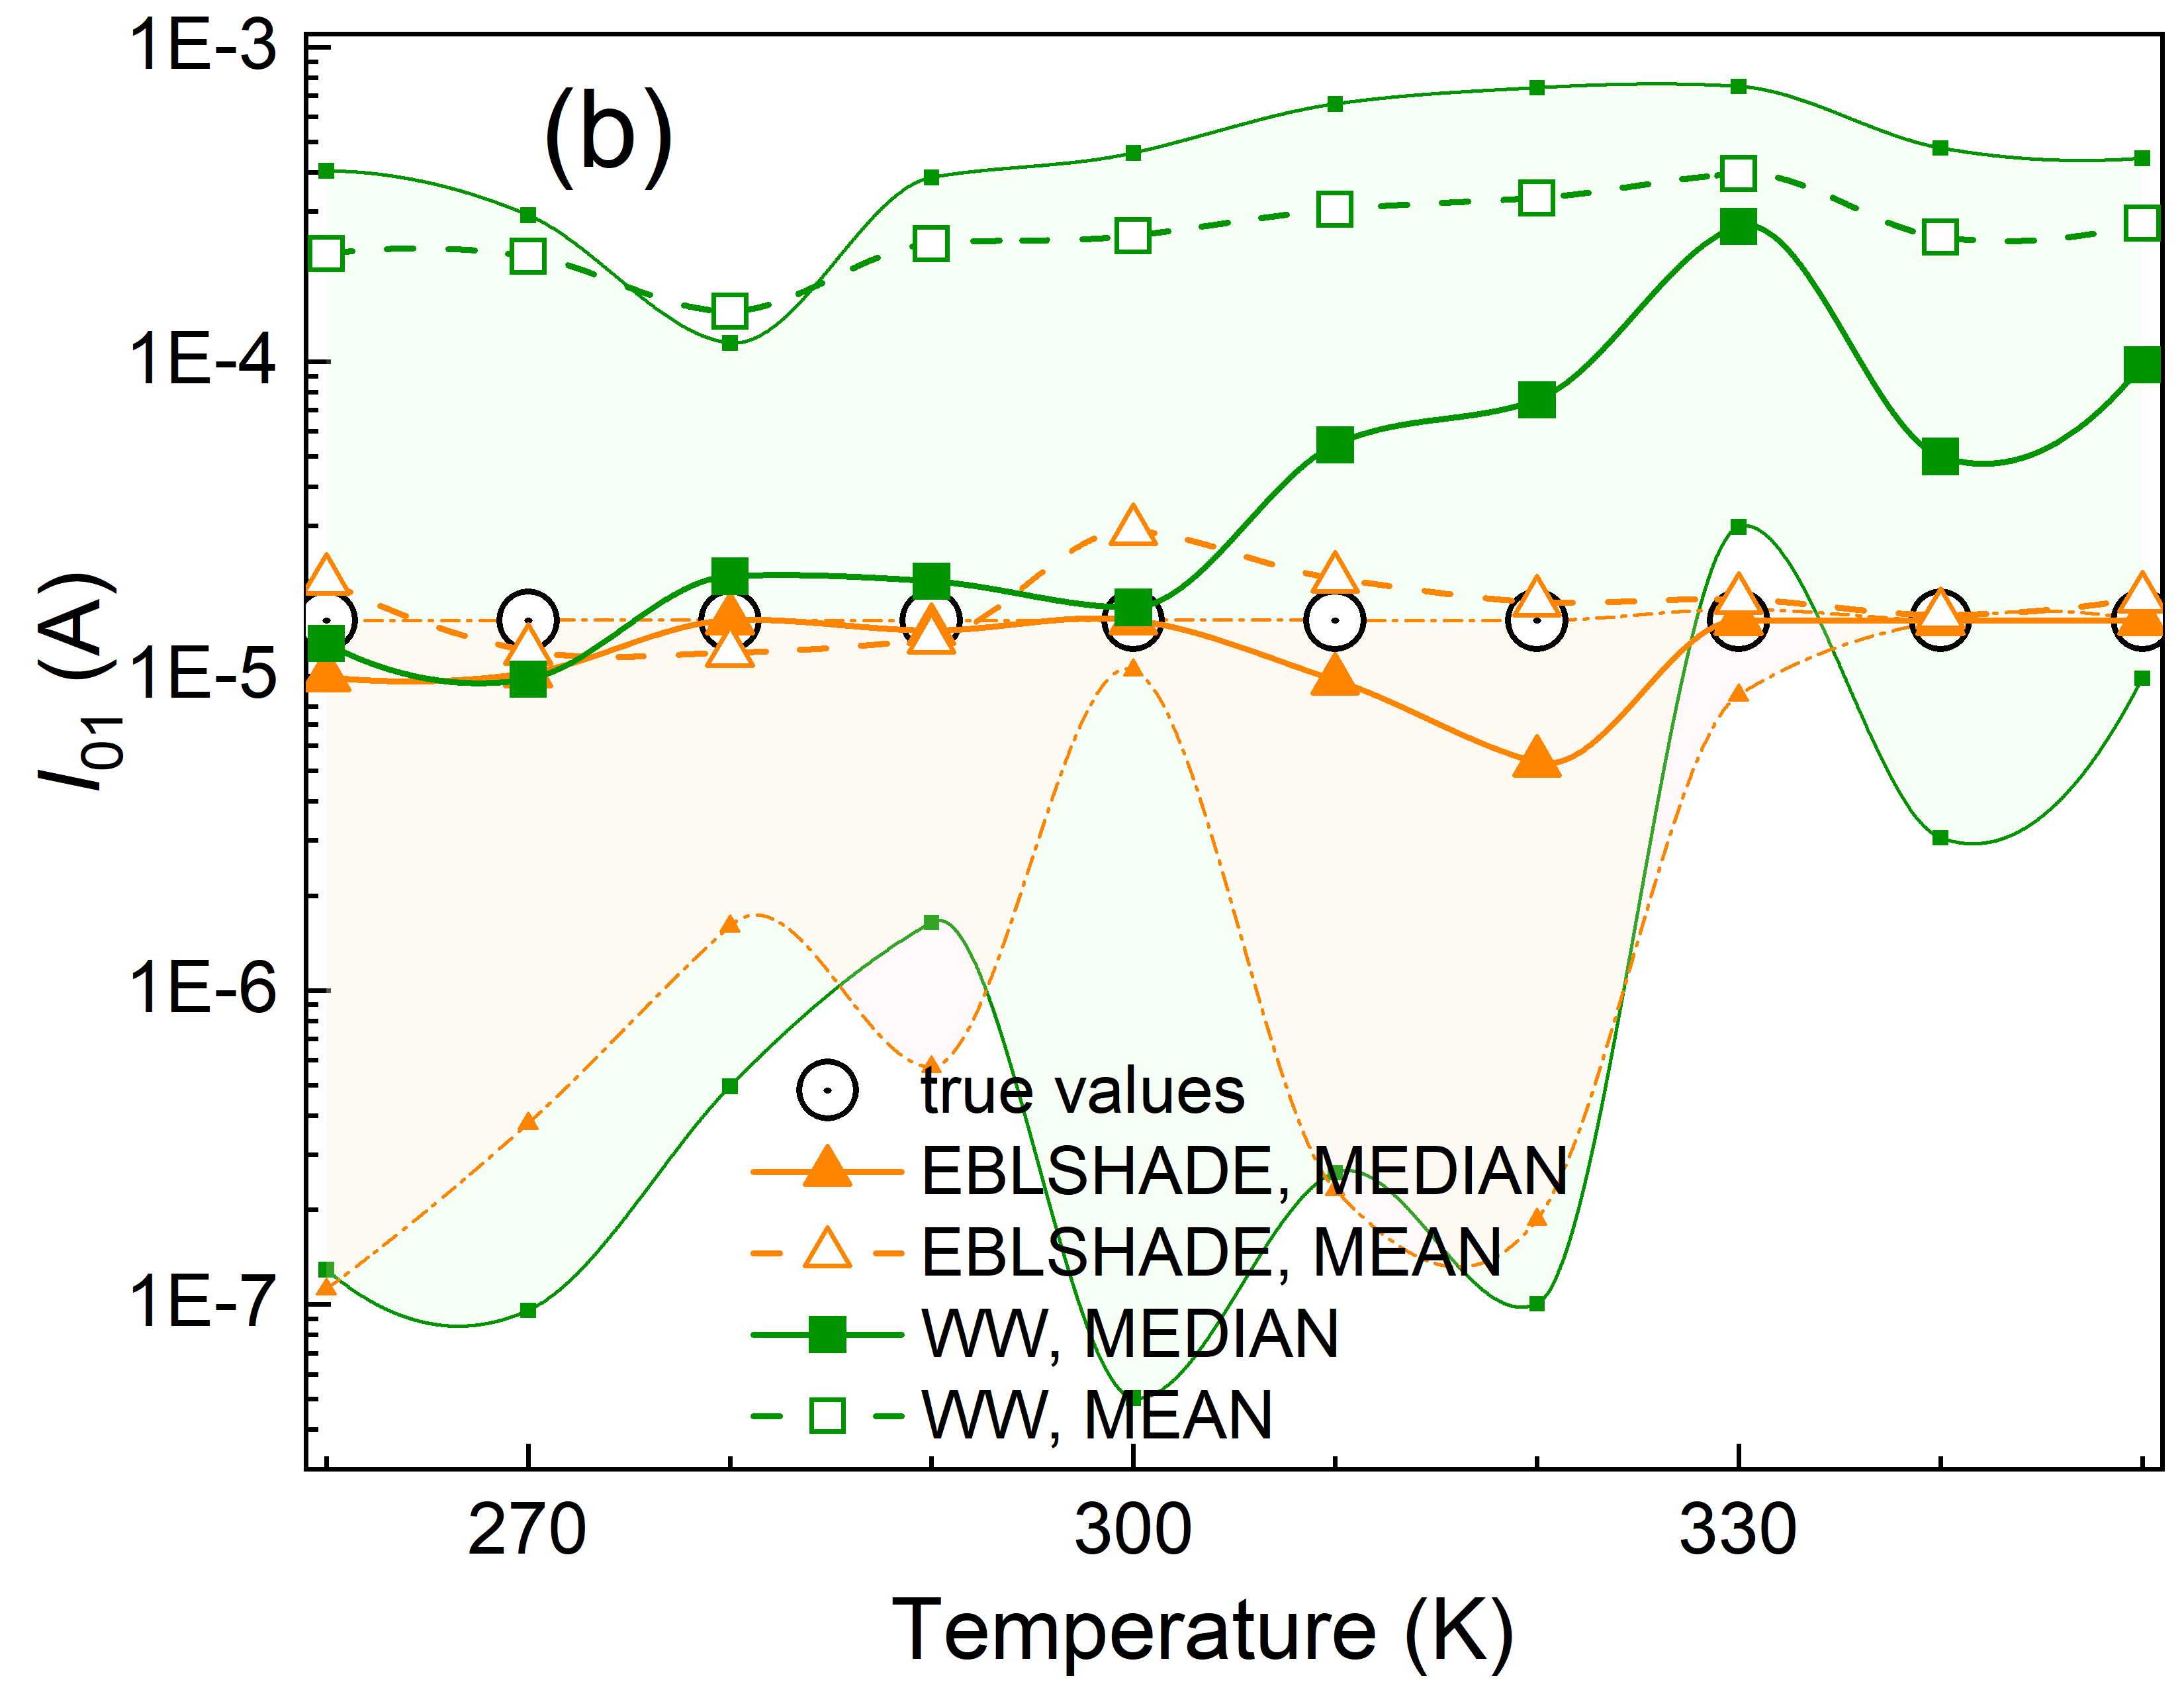
\includegraphics[width=.32\textwidth]{AfigB}
        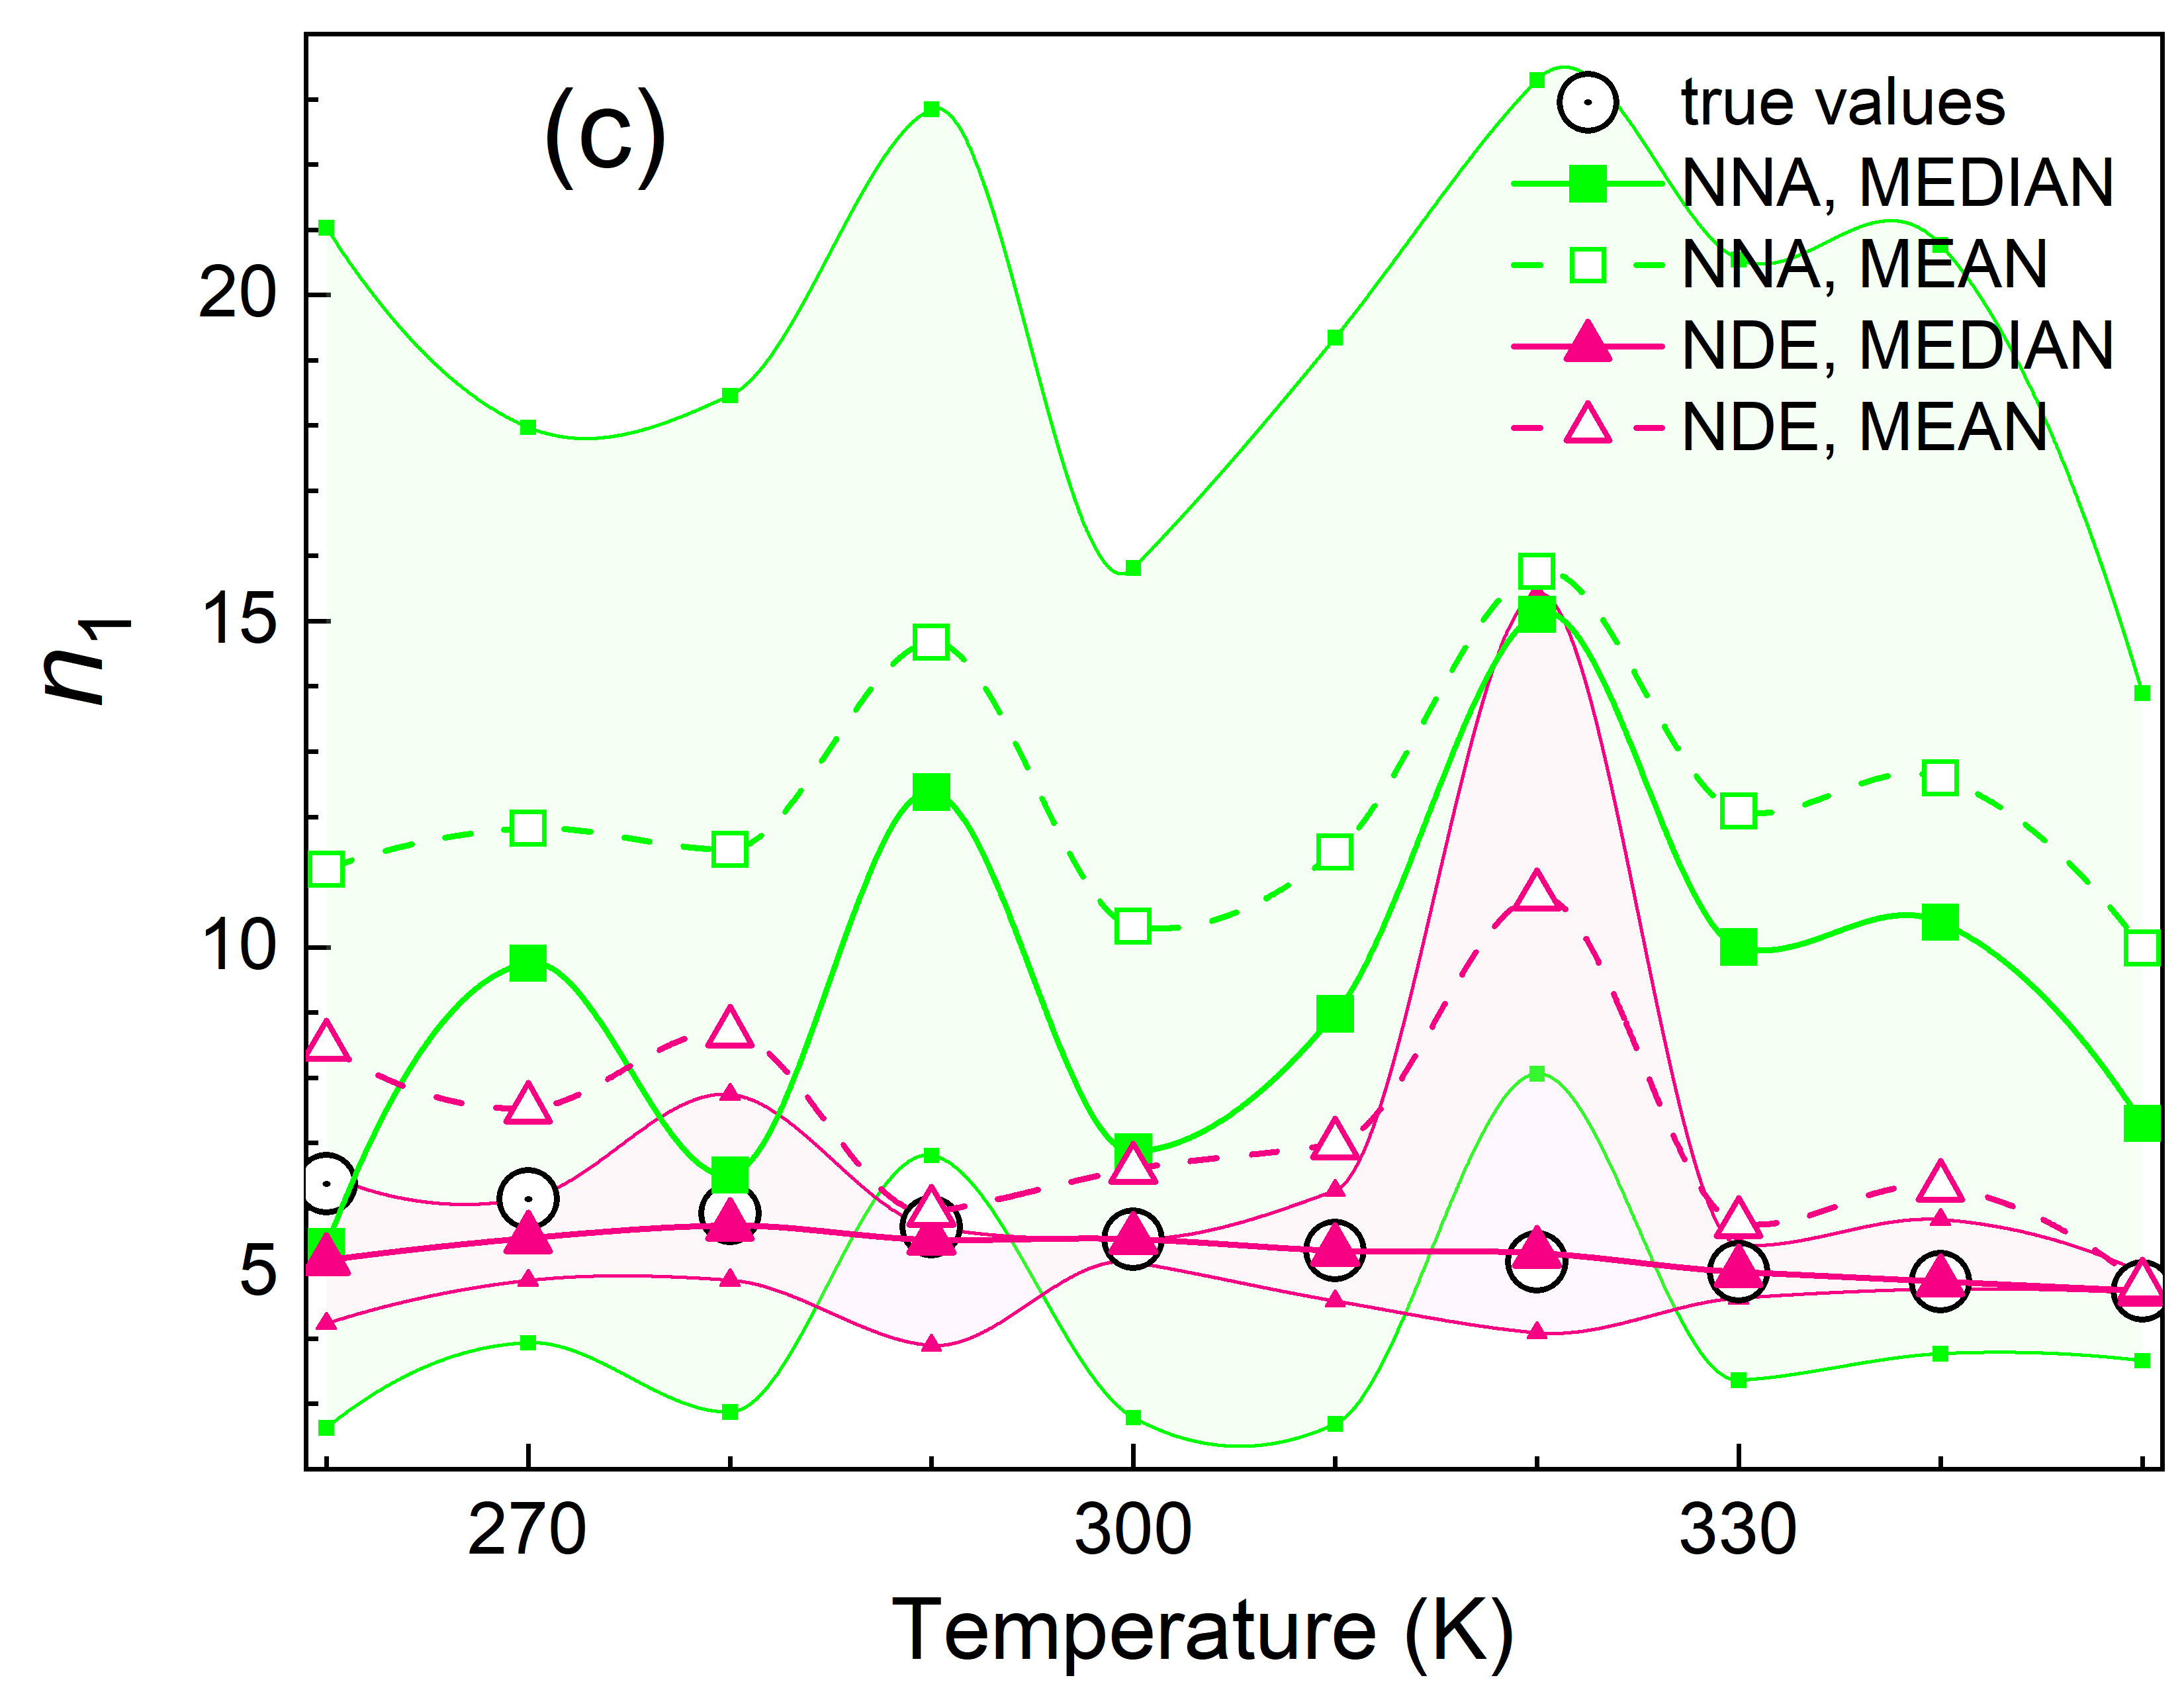
\includegraphics[width=.32\textwidth]{AfigC}
		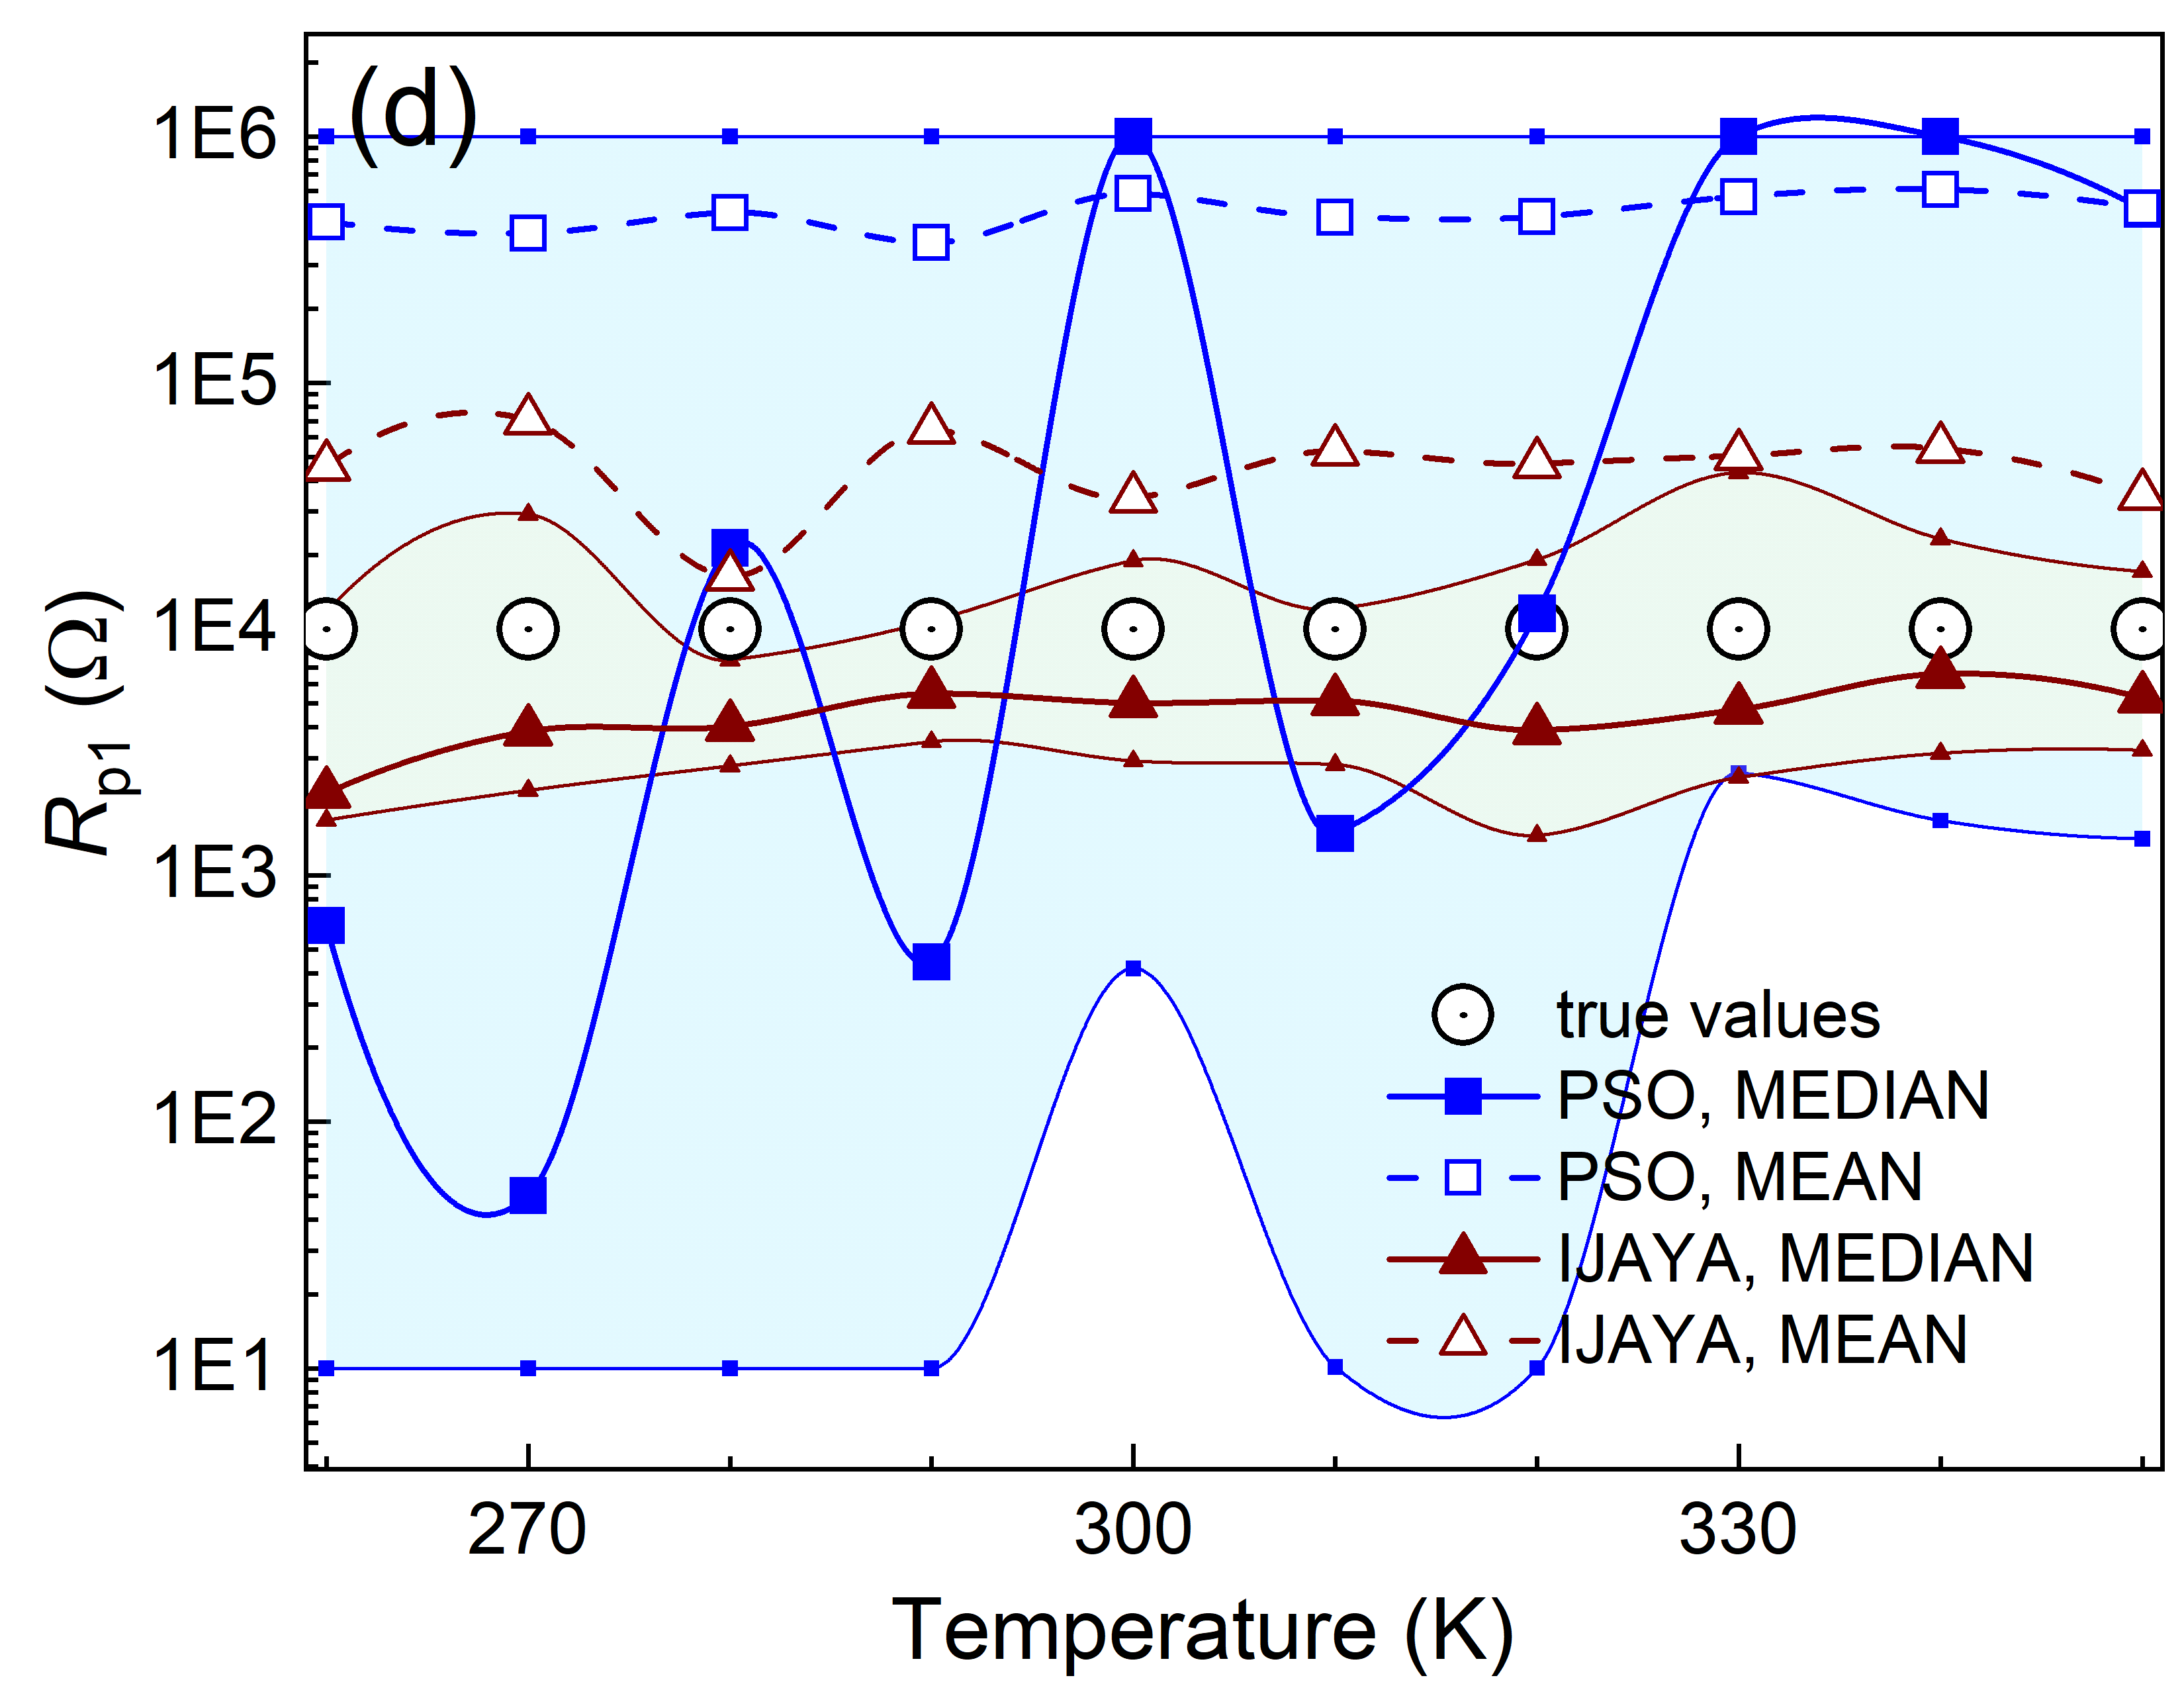
\includegraphics[width=.32\textwidth]{AfigD}
        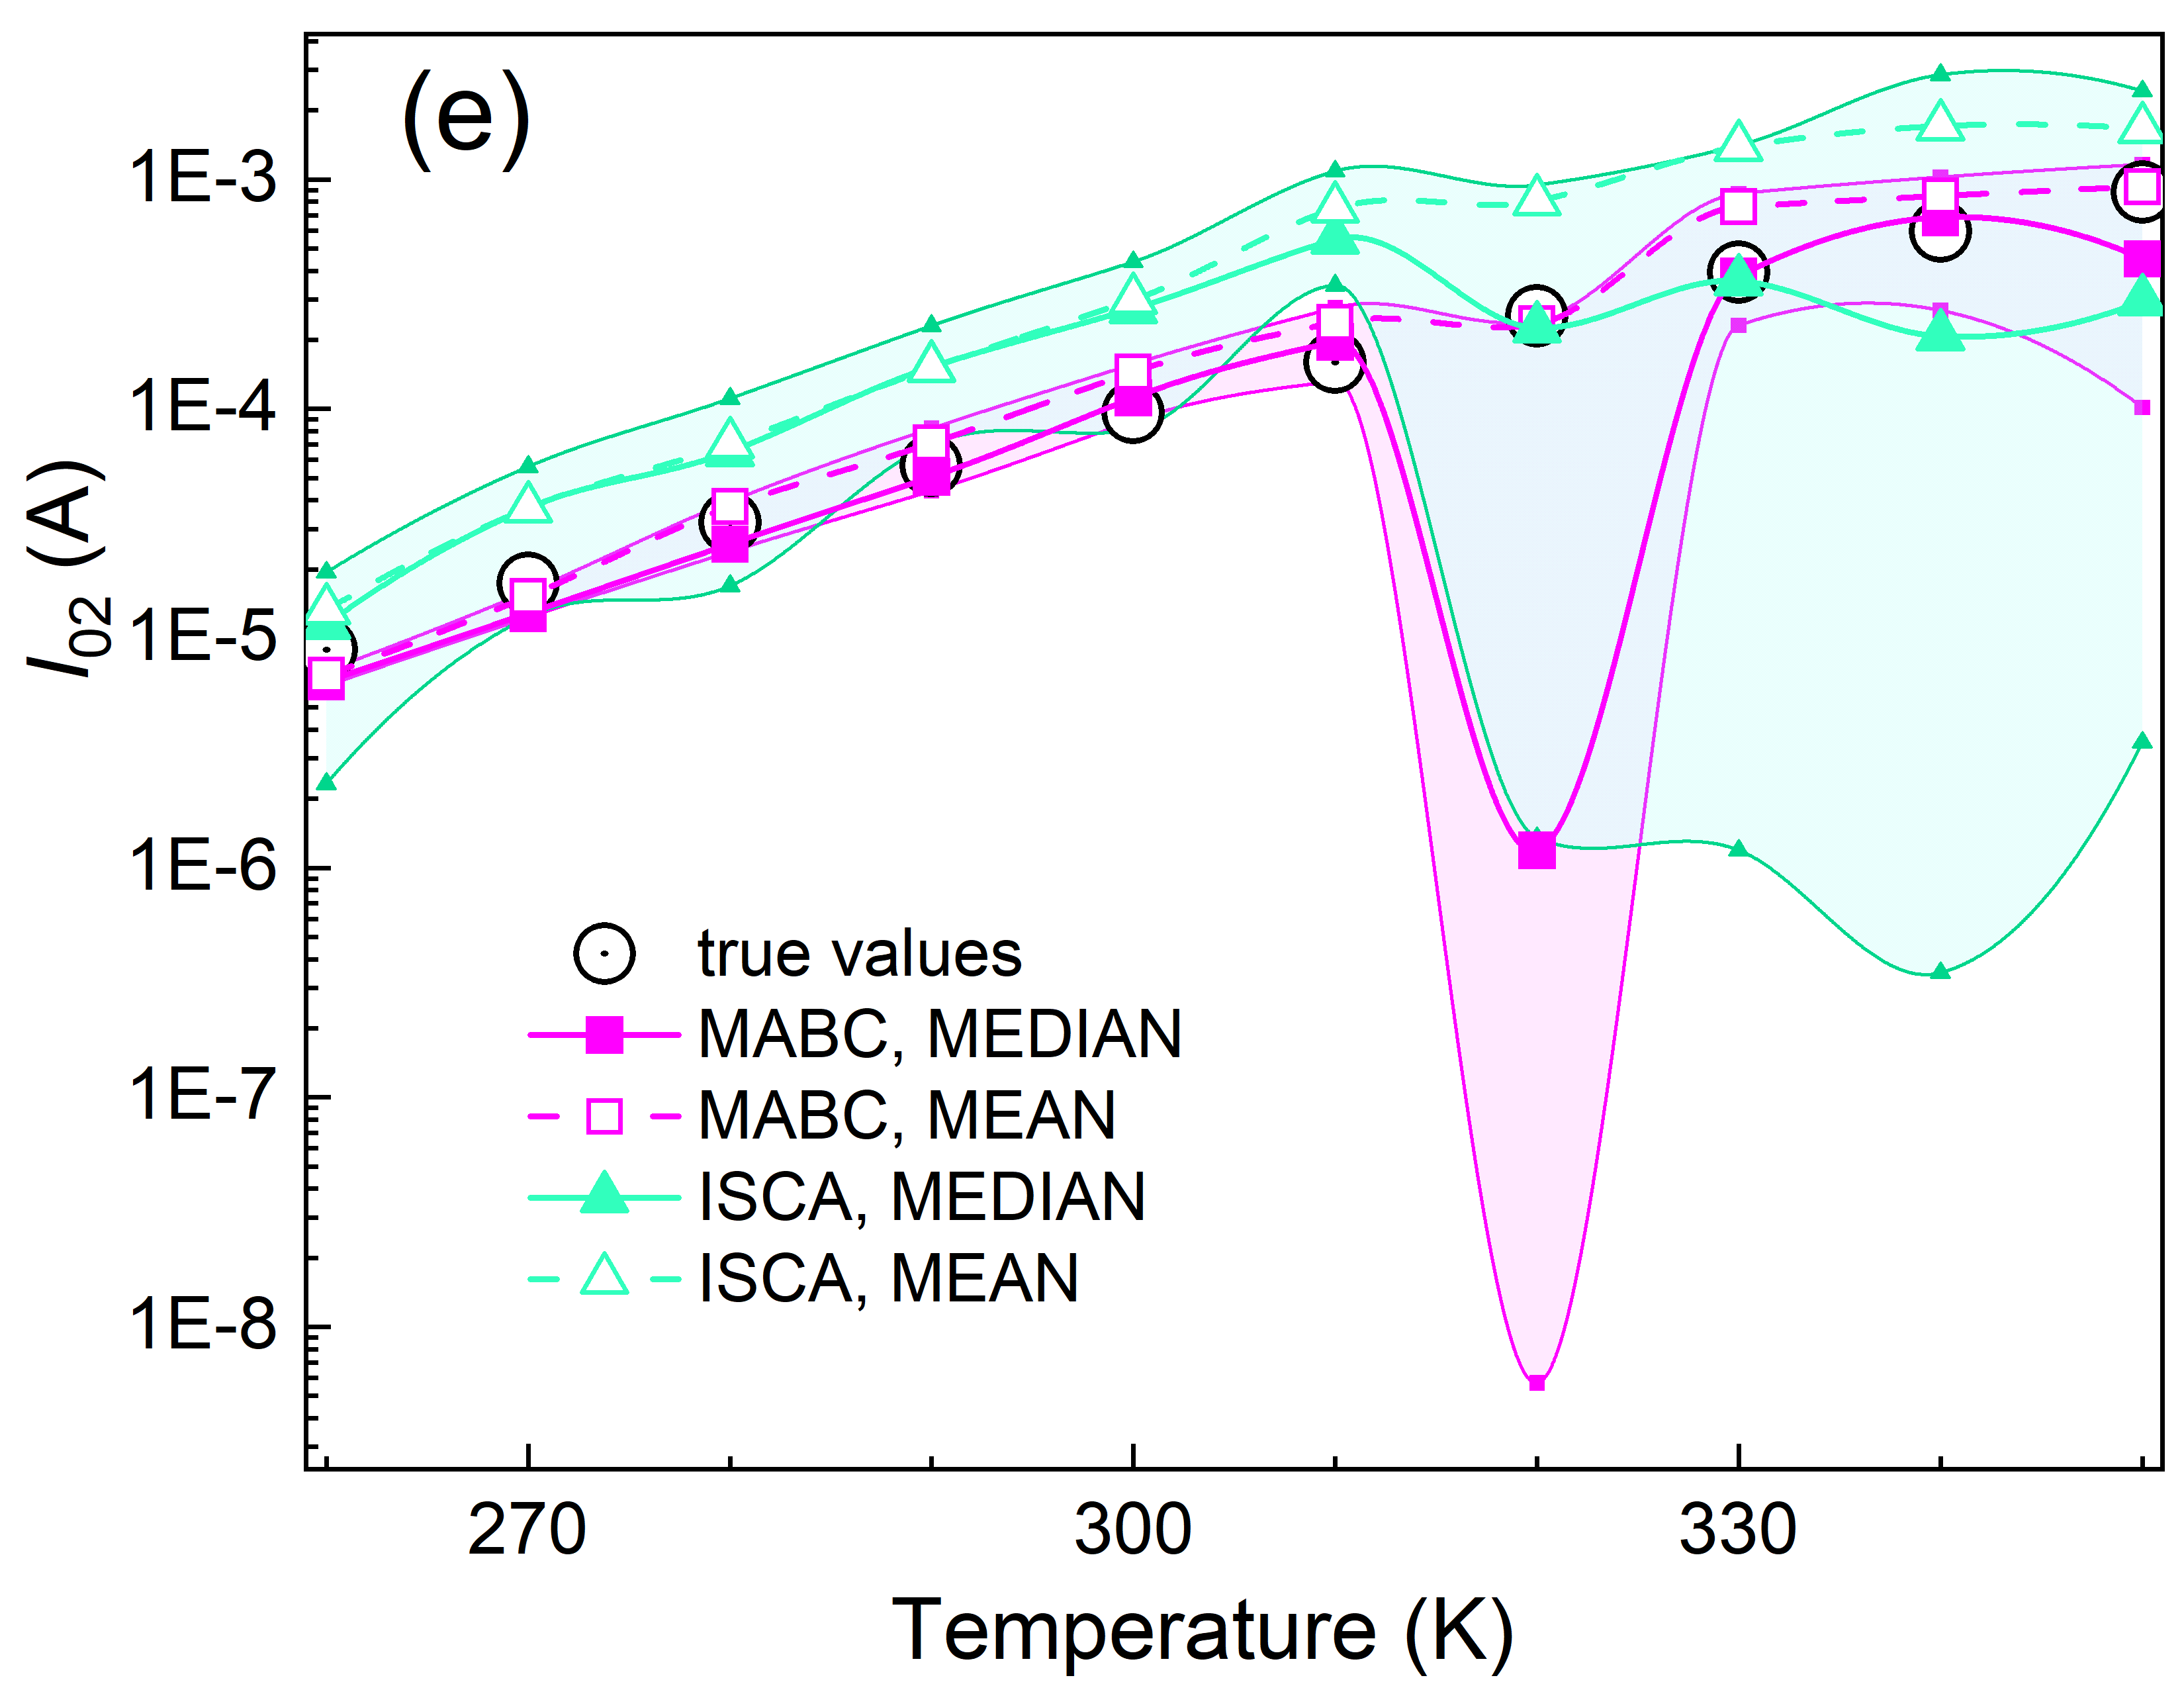
\includegraphics[width=.32\textwidth]{AfigE}
        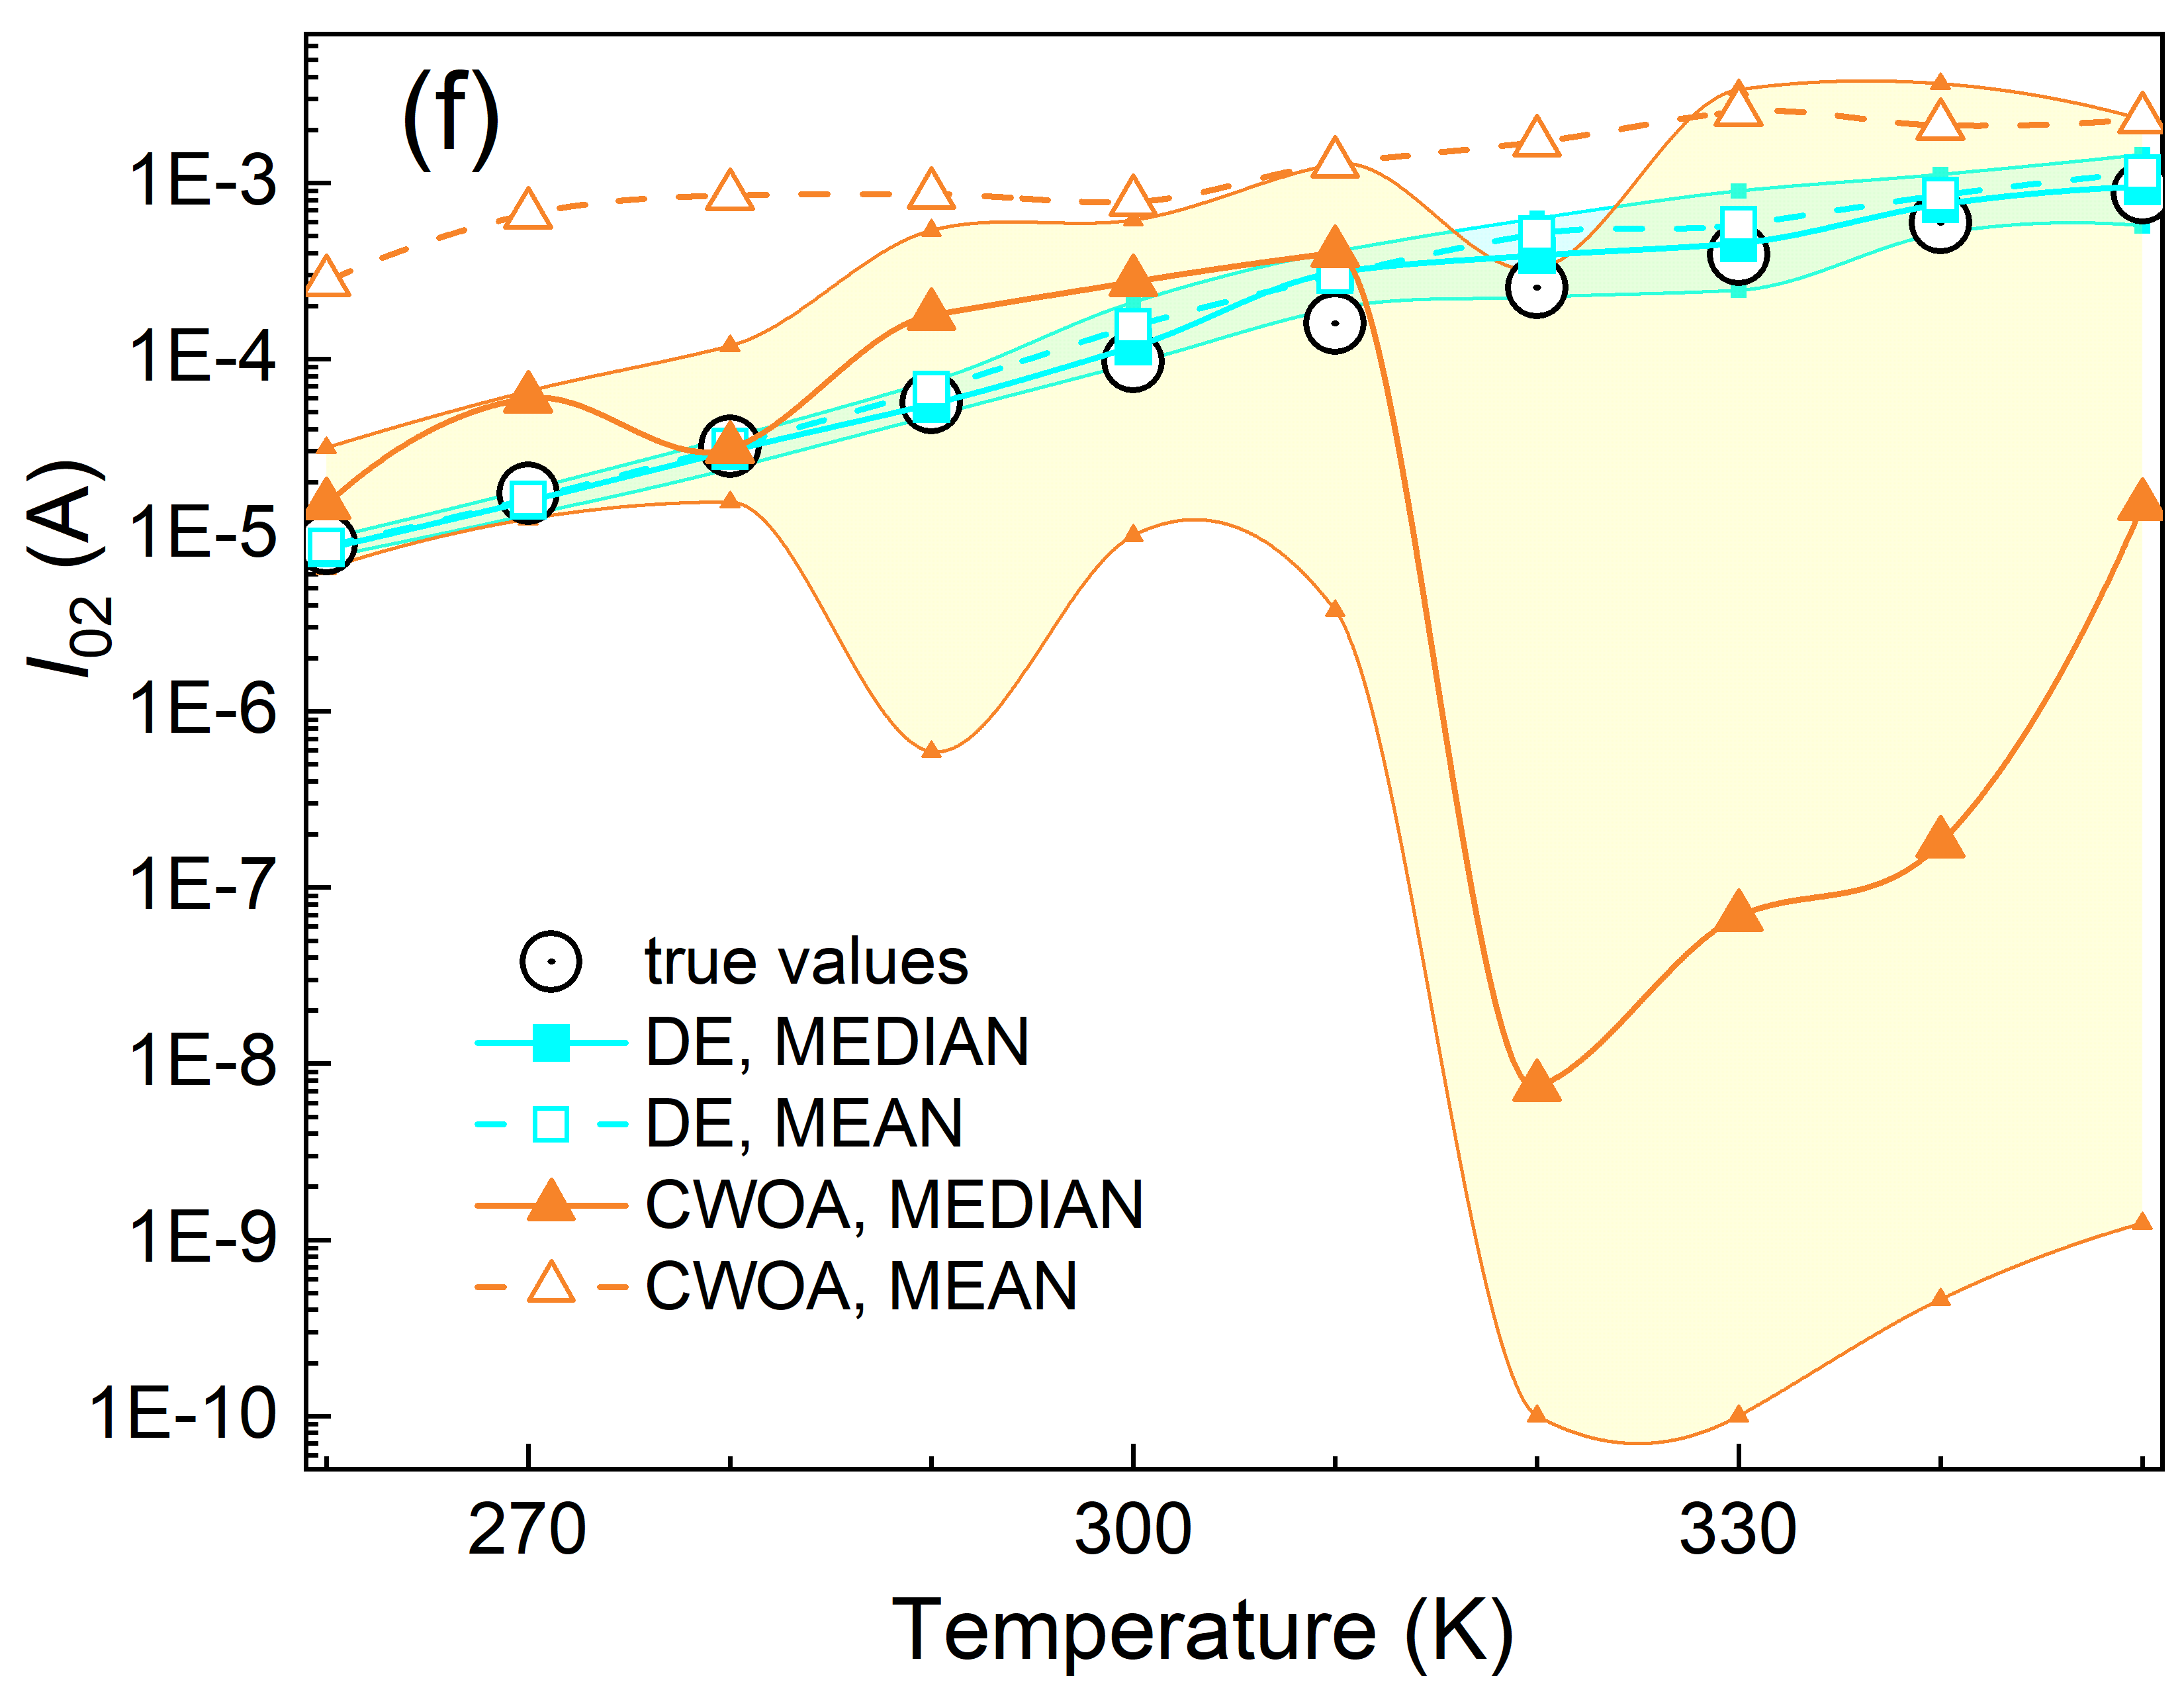
\includegraphics[width=.32\textwidth]{AfigF}
		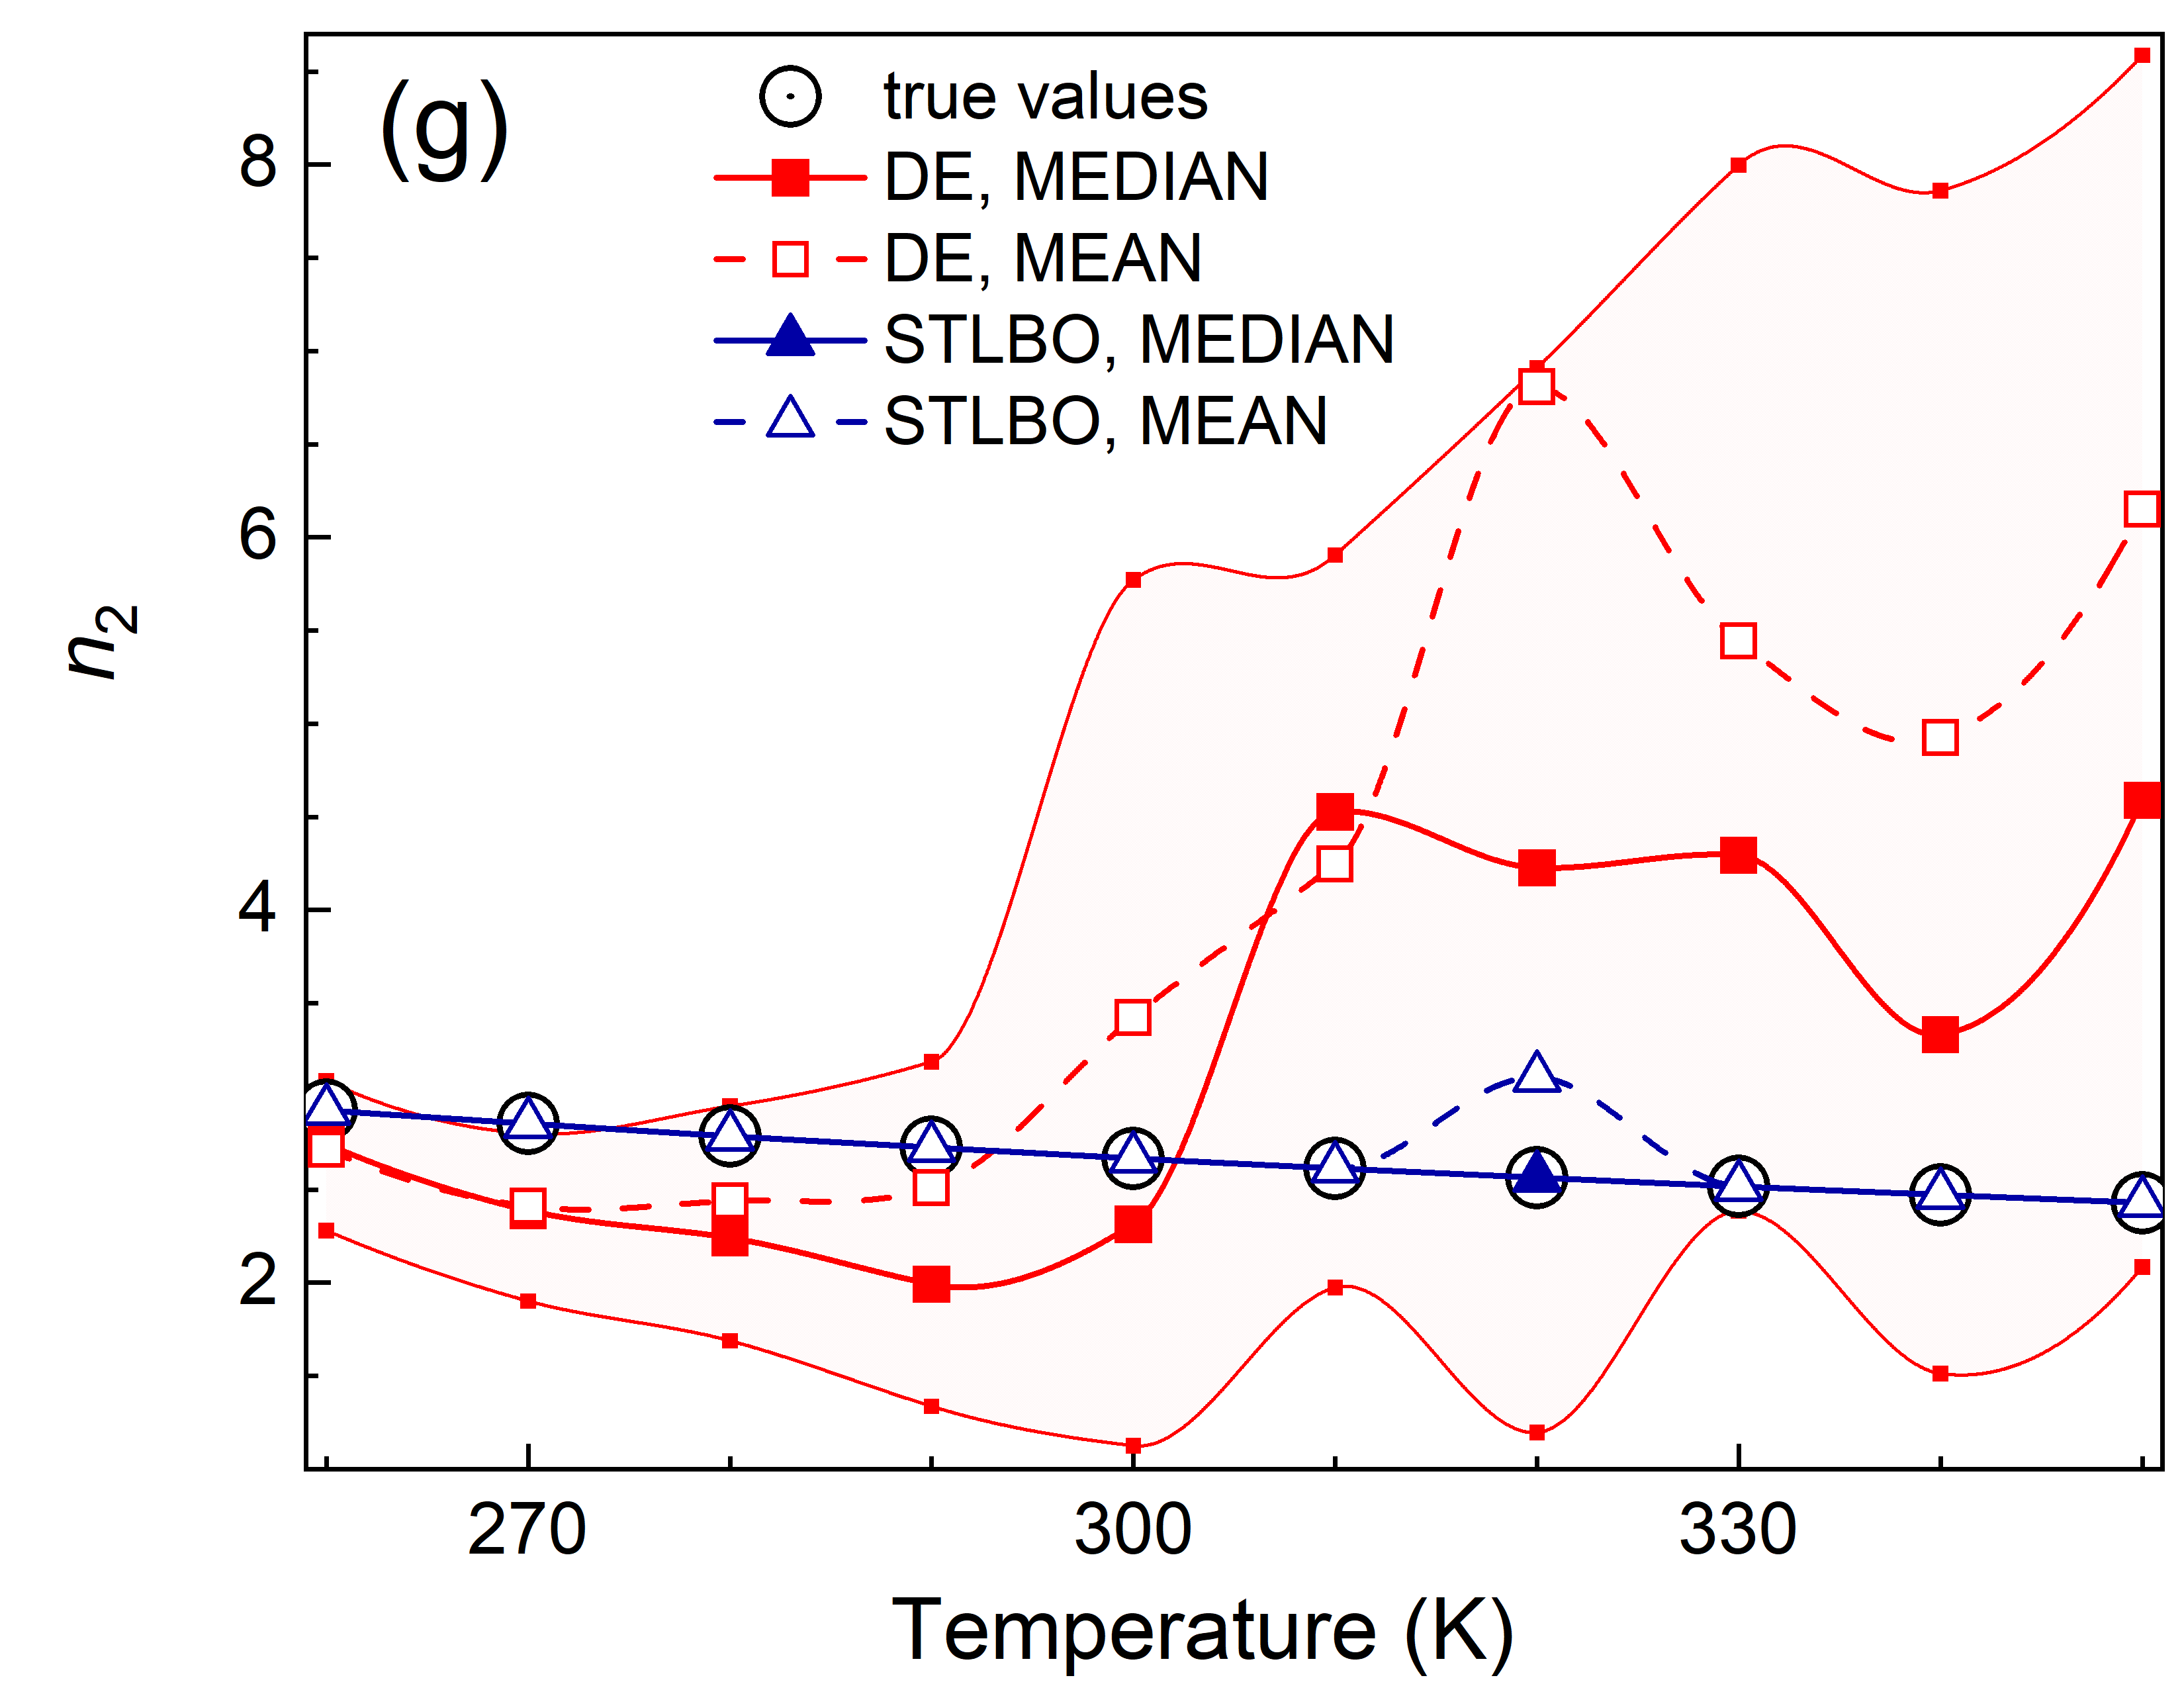
\includegraphics[width=.32\textwidth]{AfigG}
        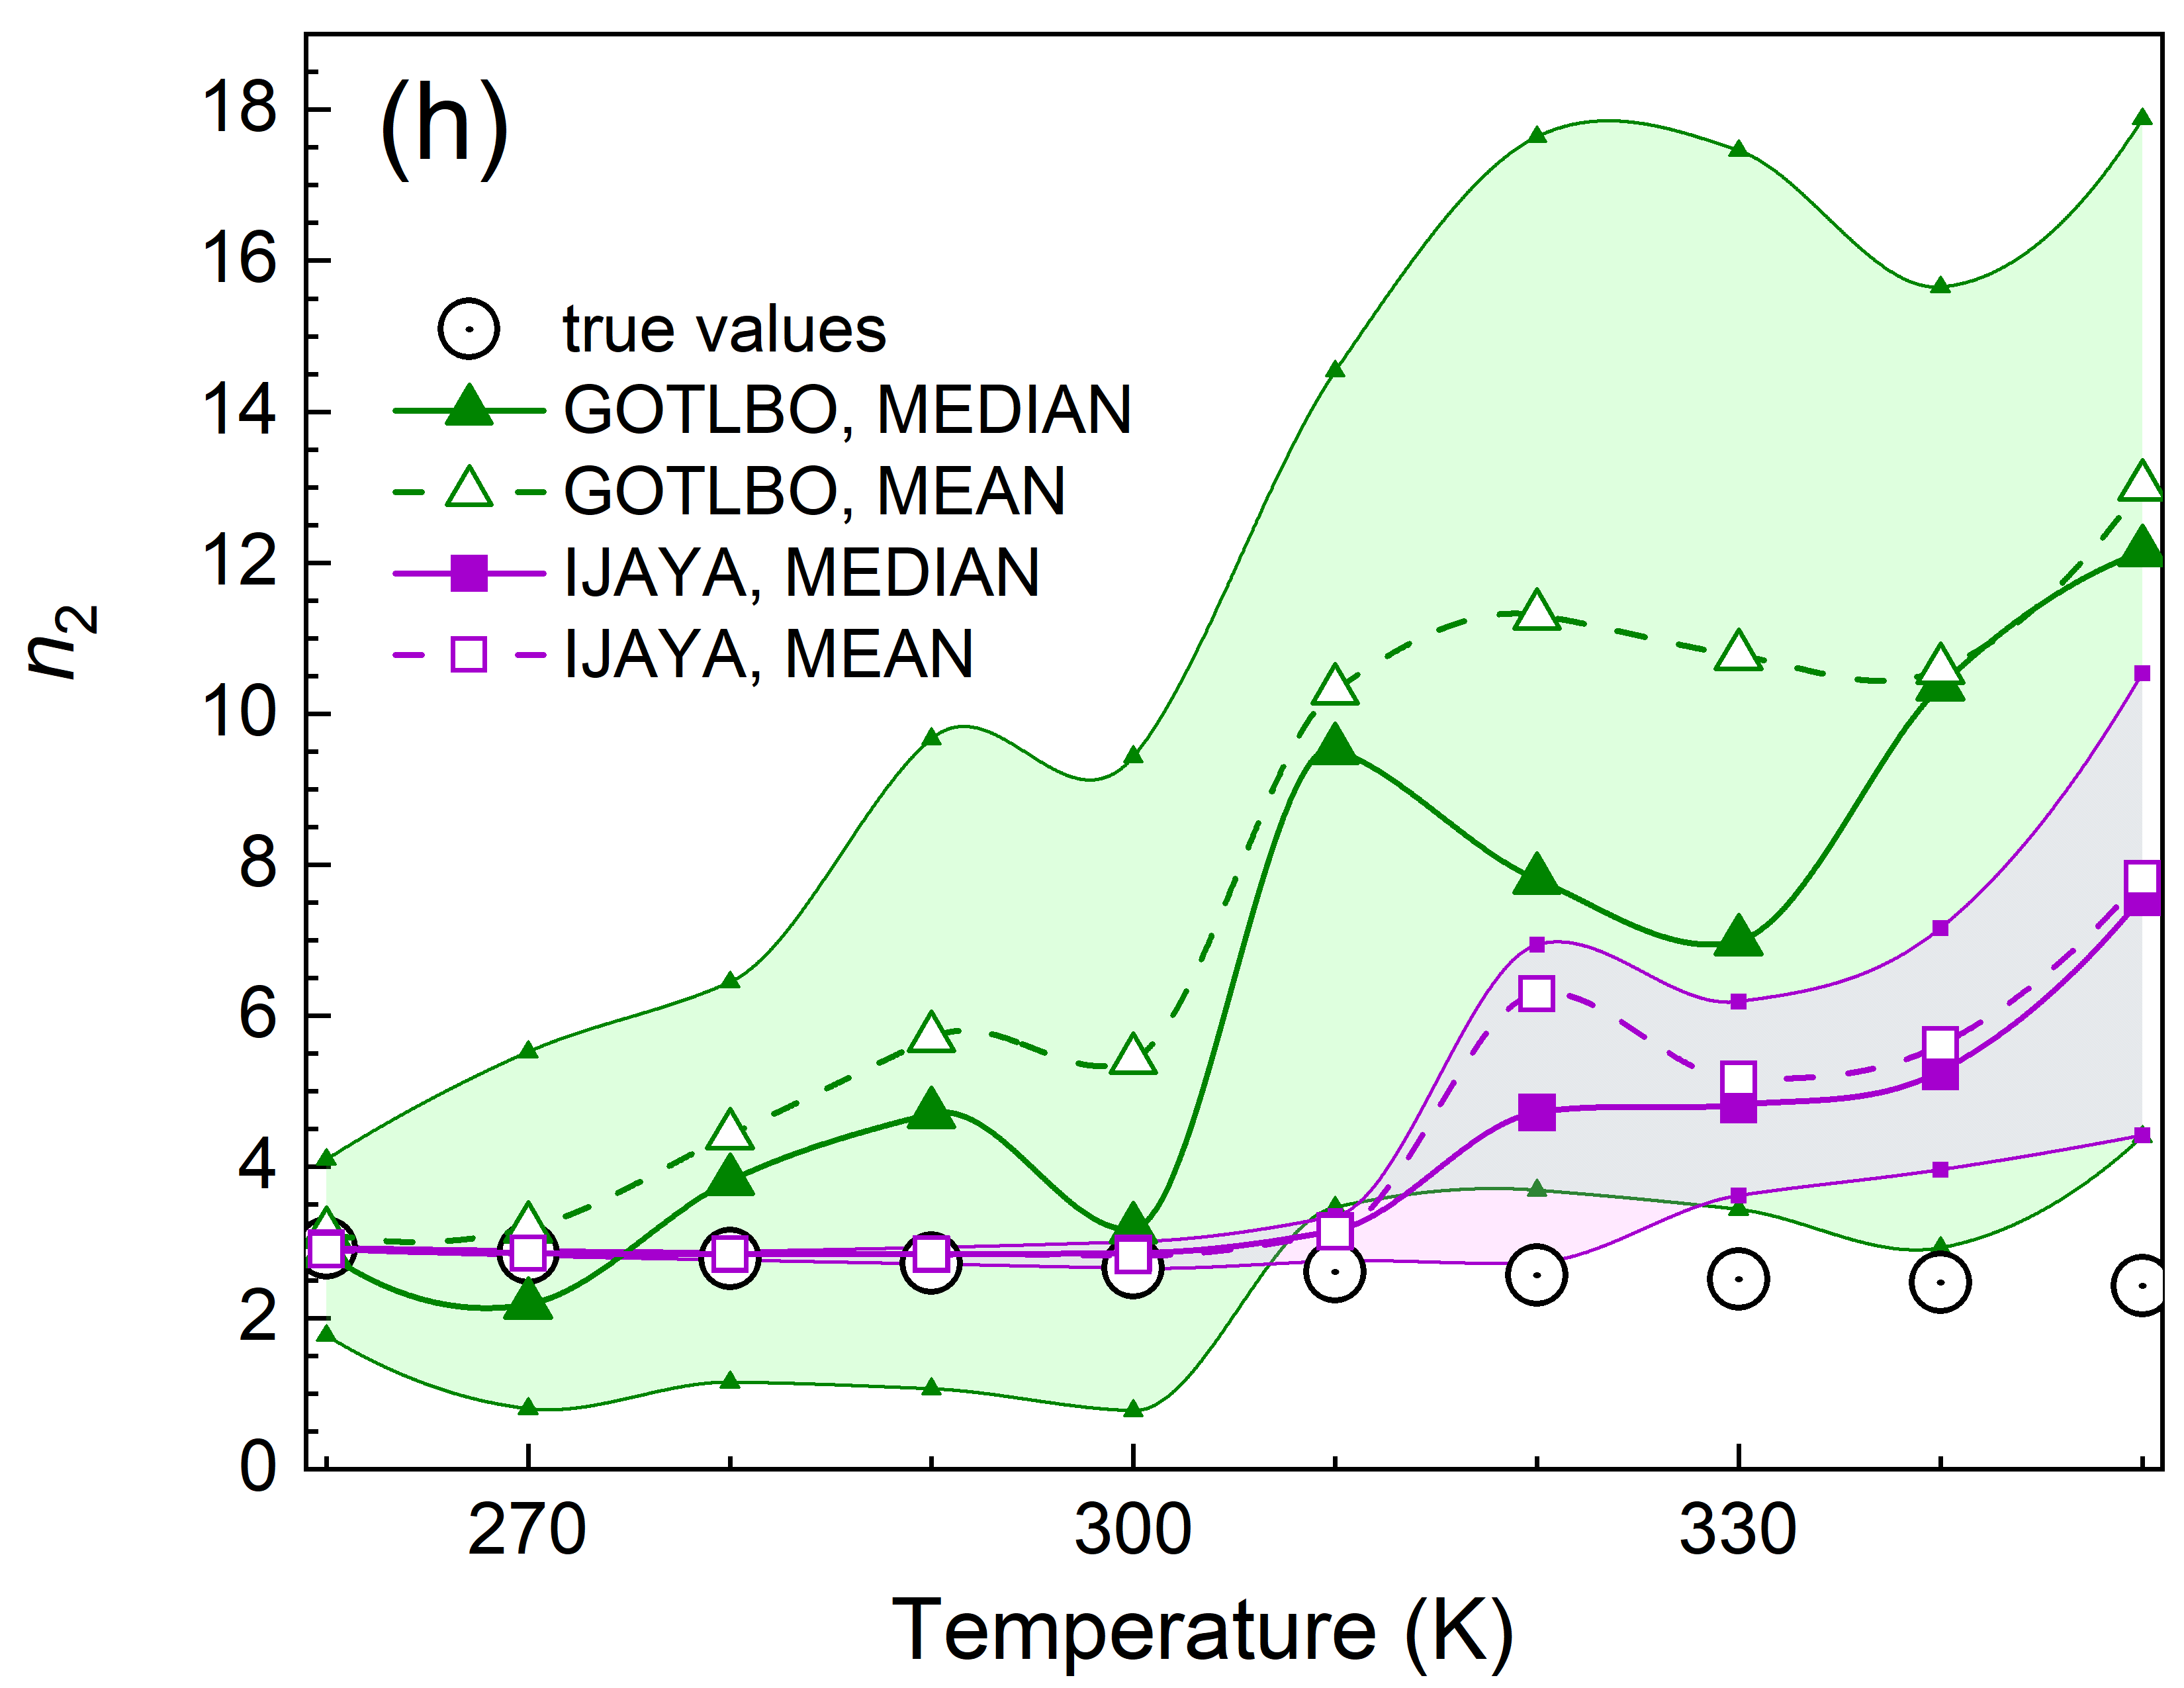
\includegraphics[width=.32\textwidth]{AfigH}
        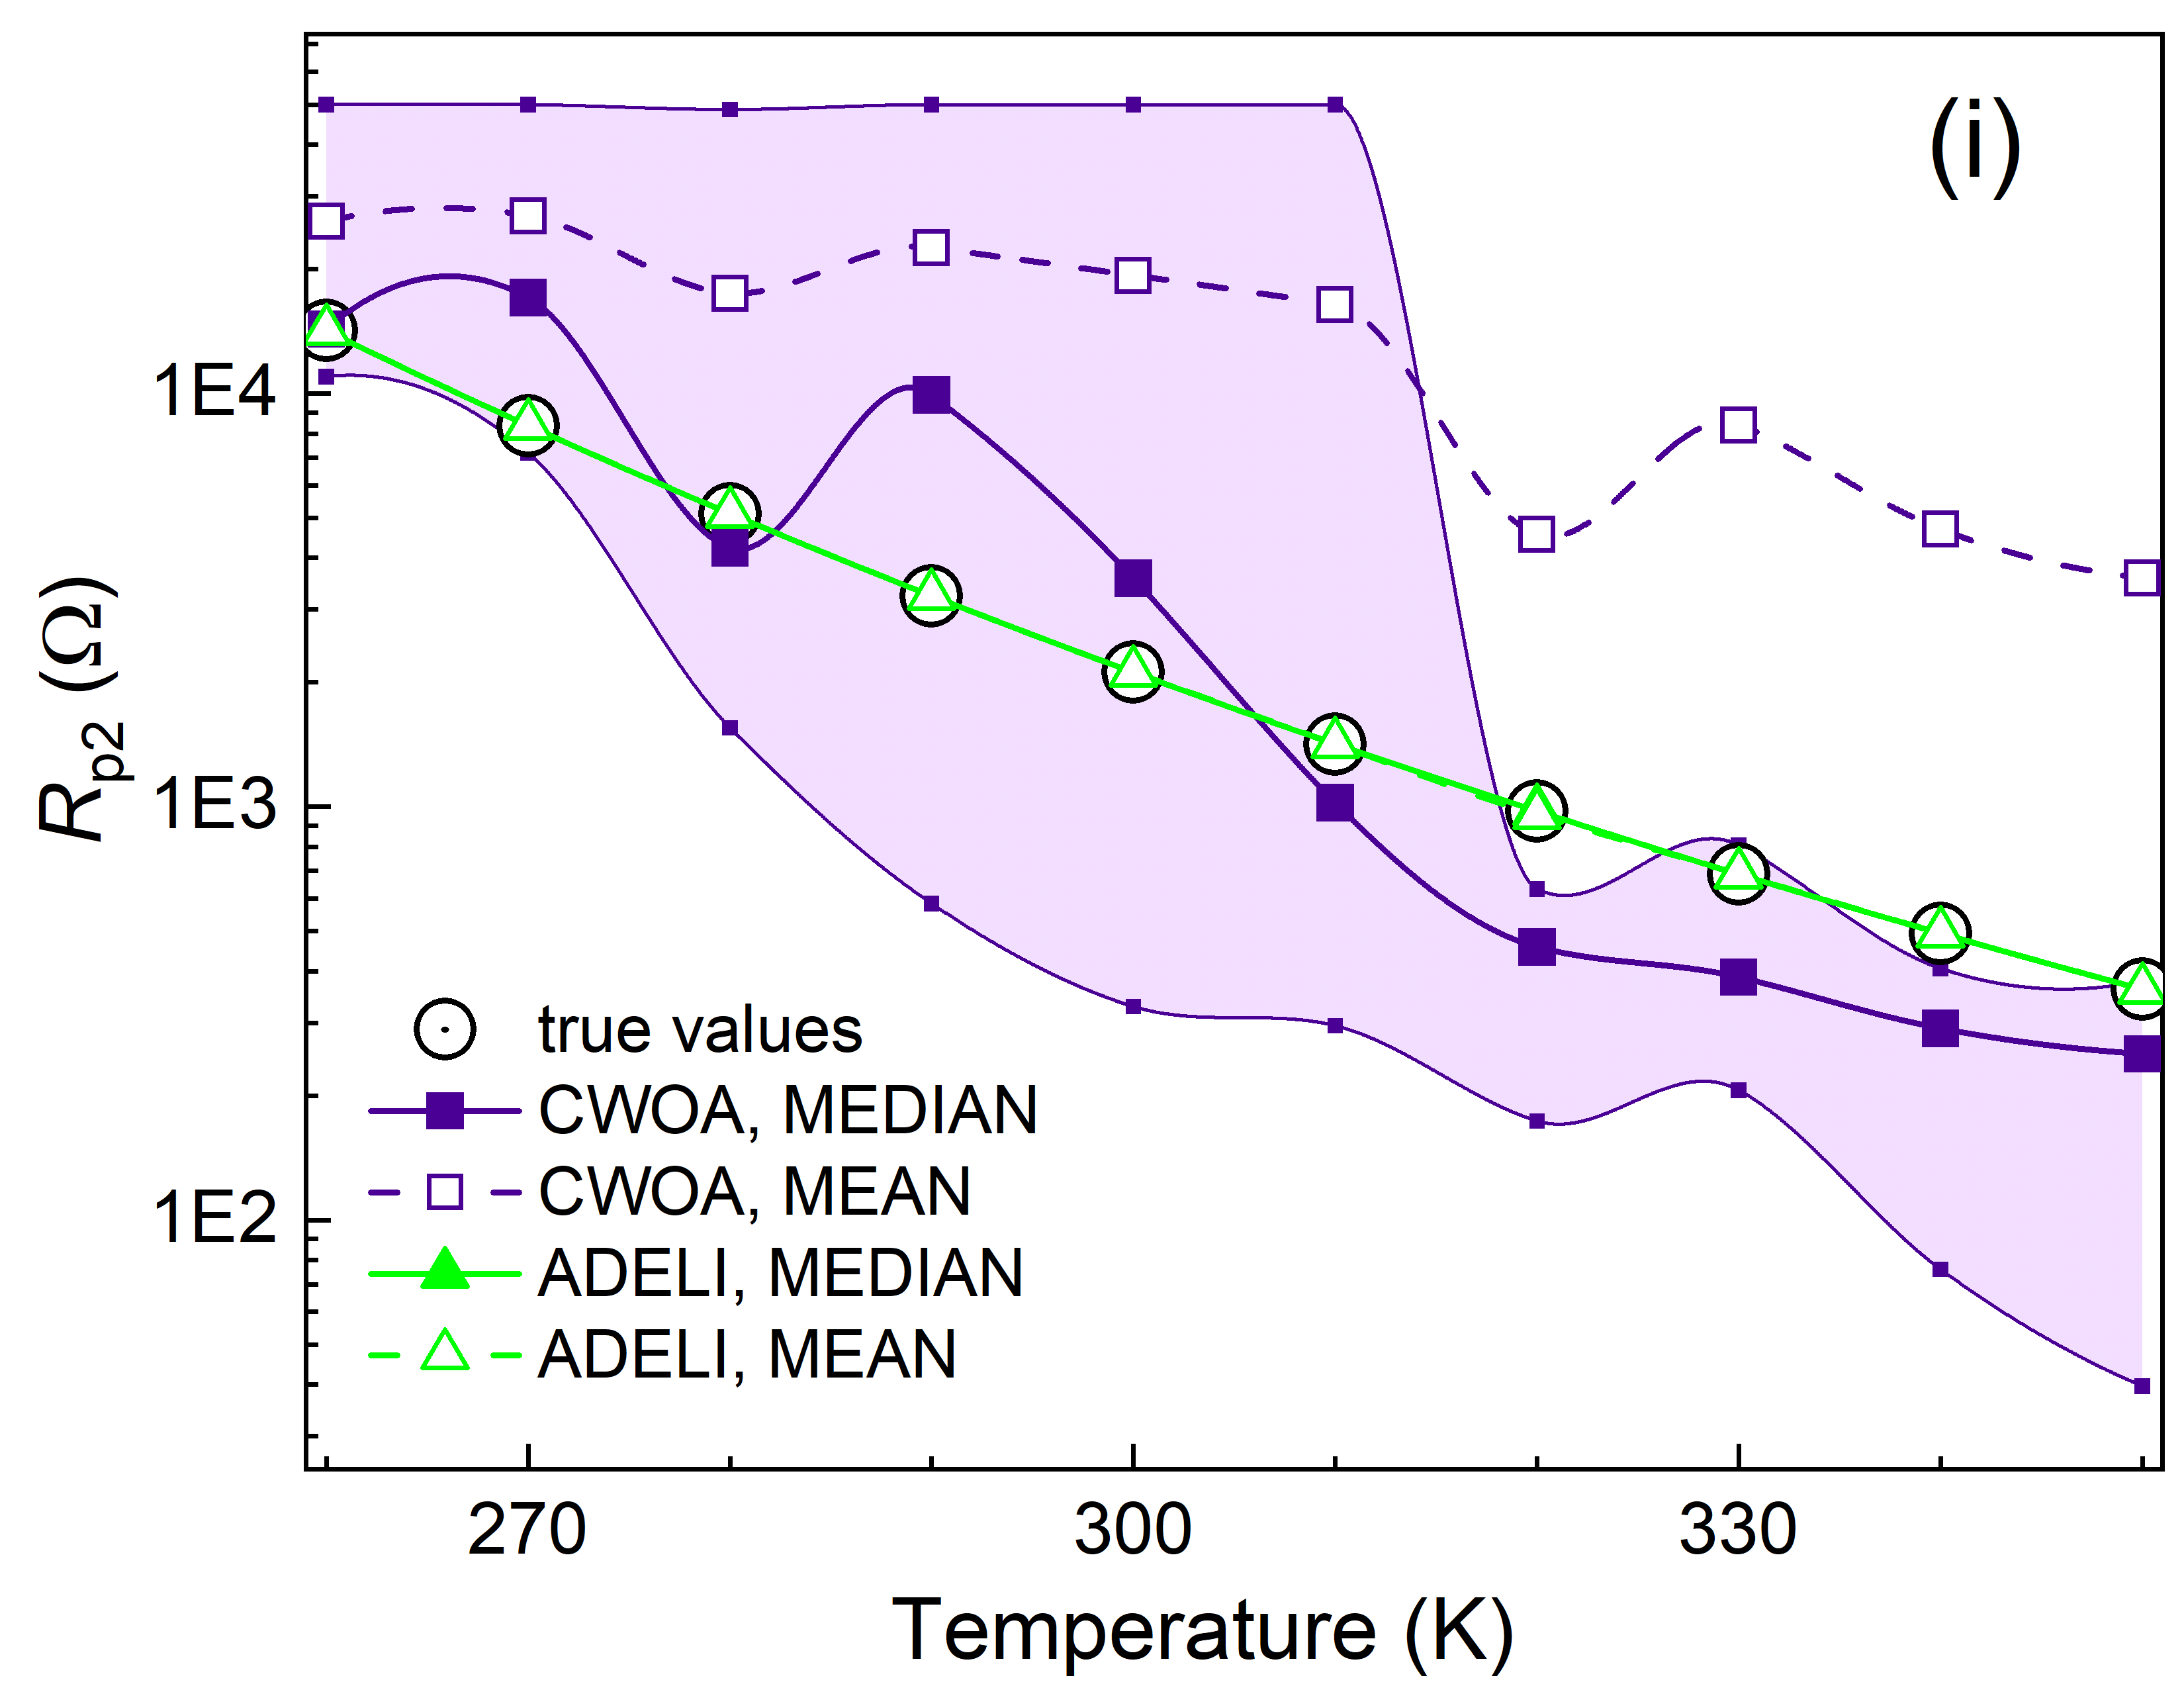
\includegraphics[width=.32\textwidth]{AfigI}
		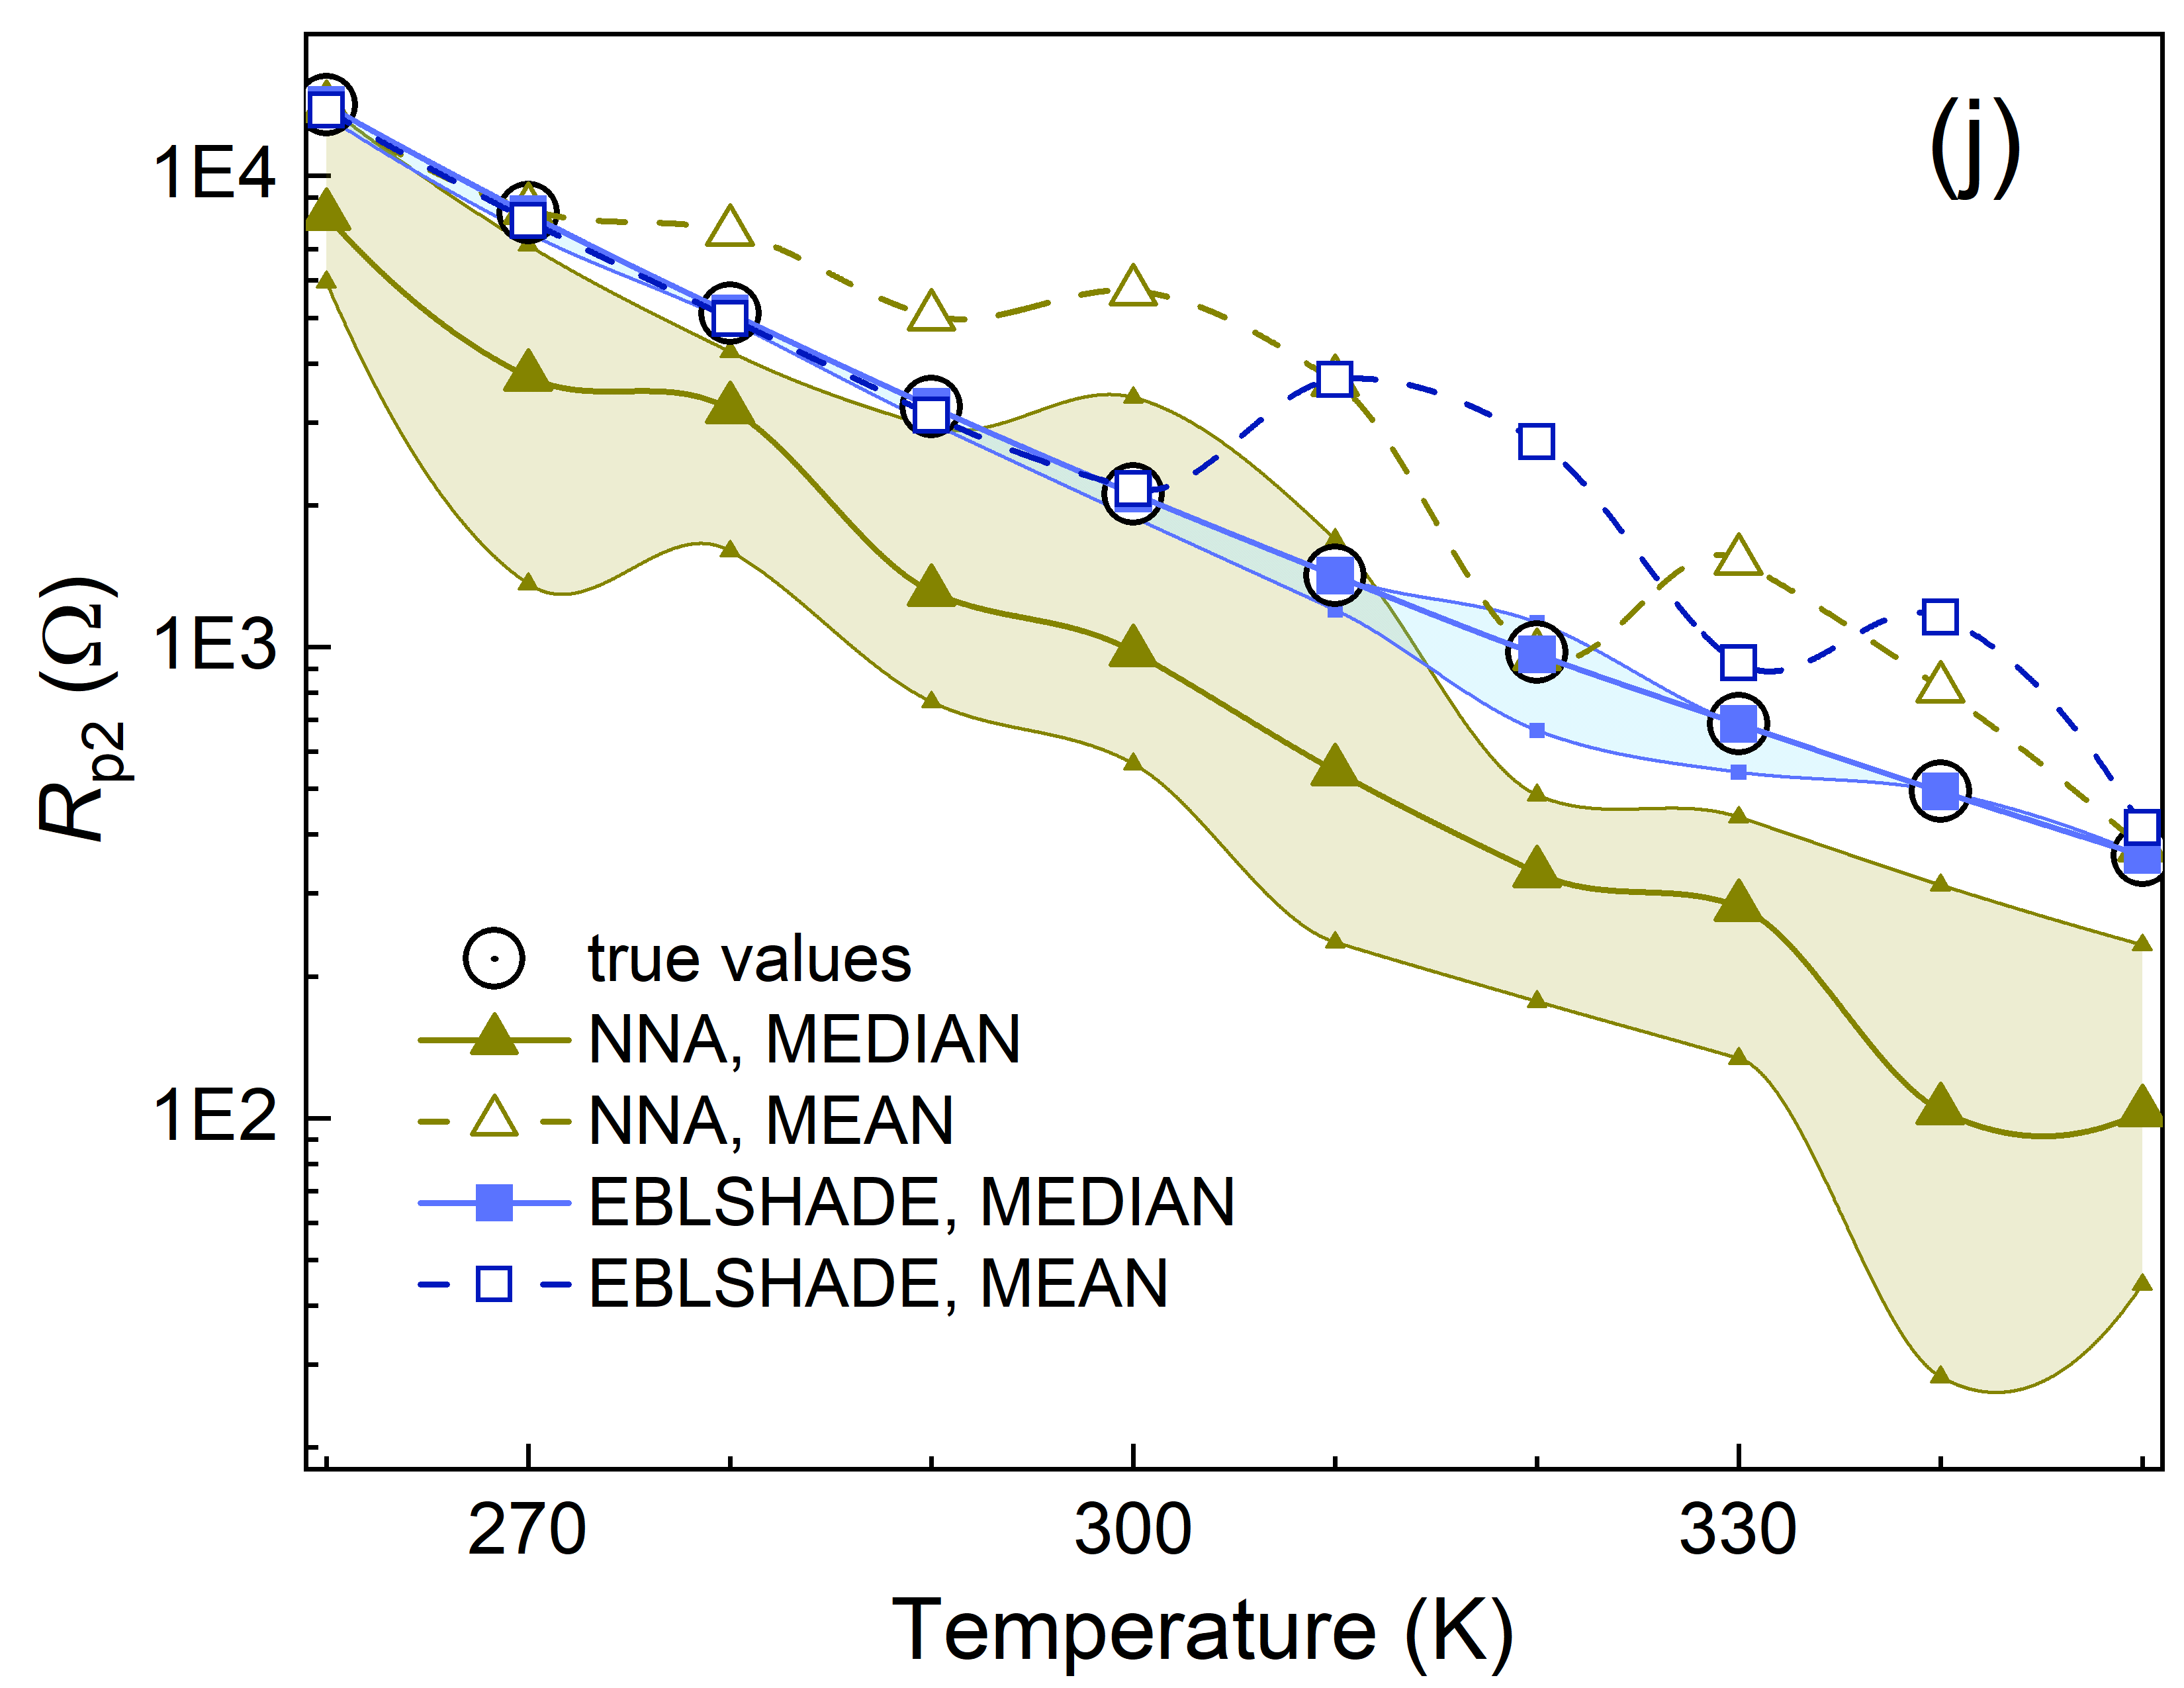
\includegraphics[width=.32\textwidth]{AfigJ}
        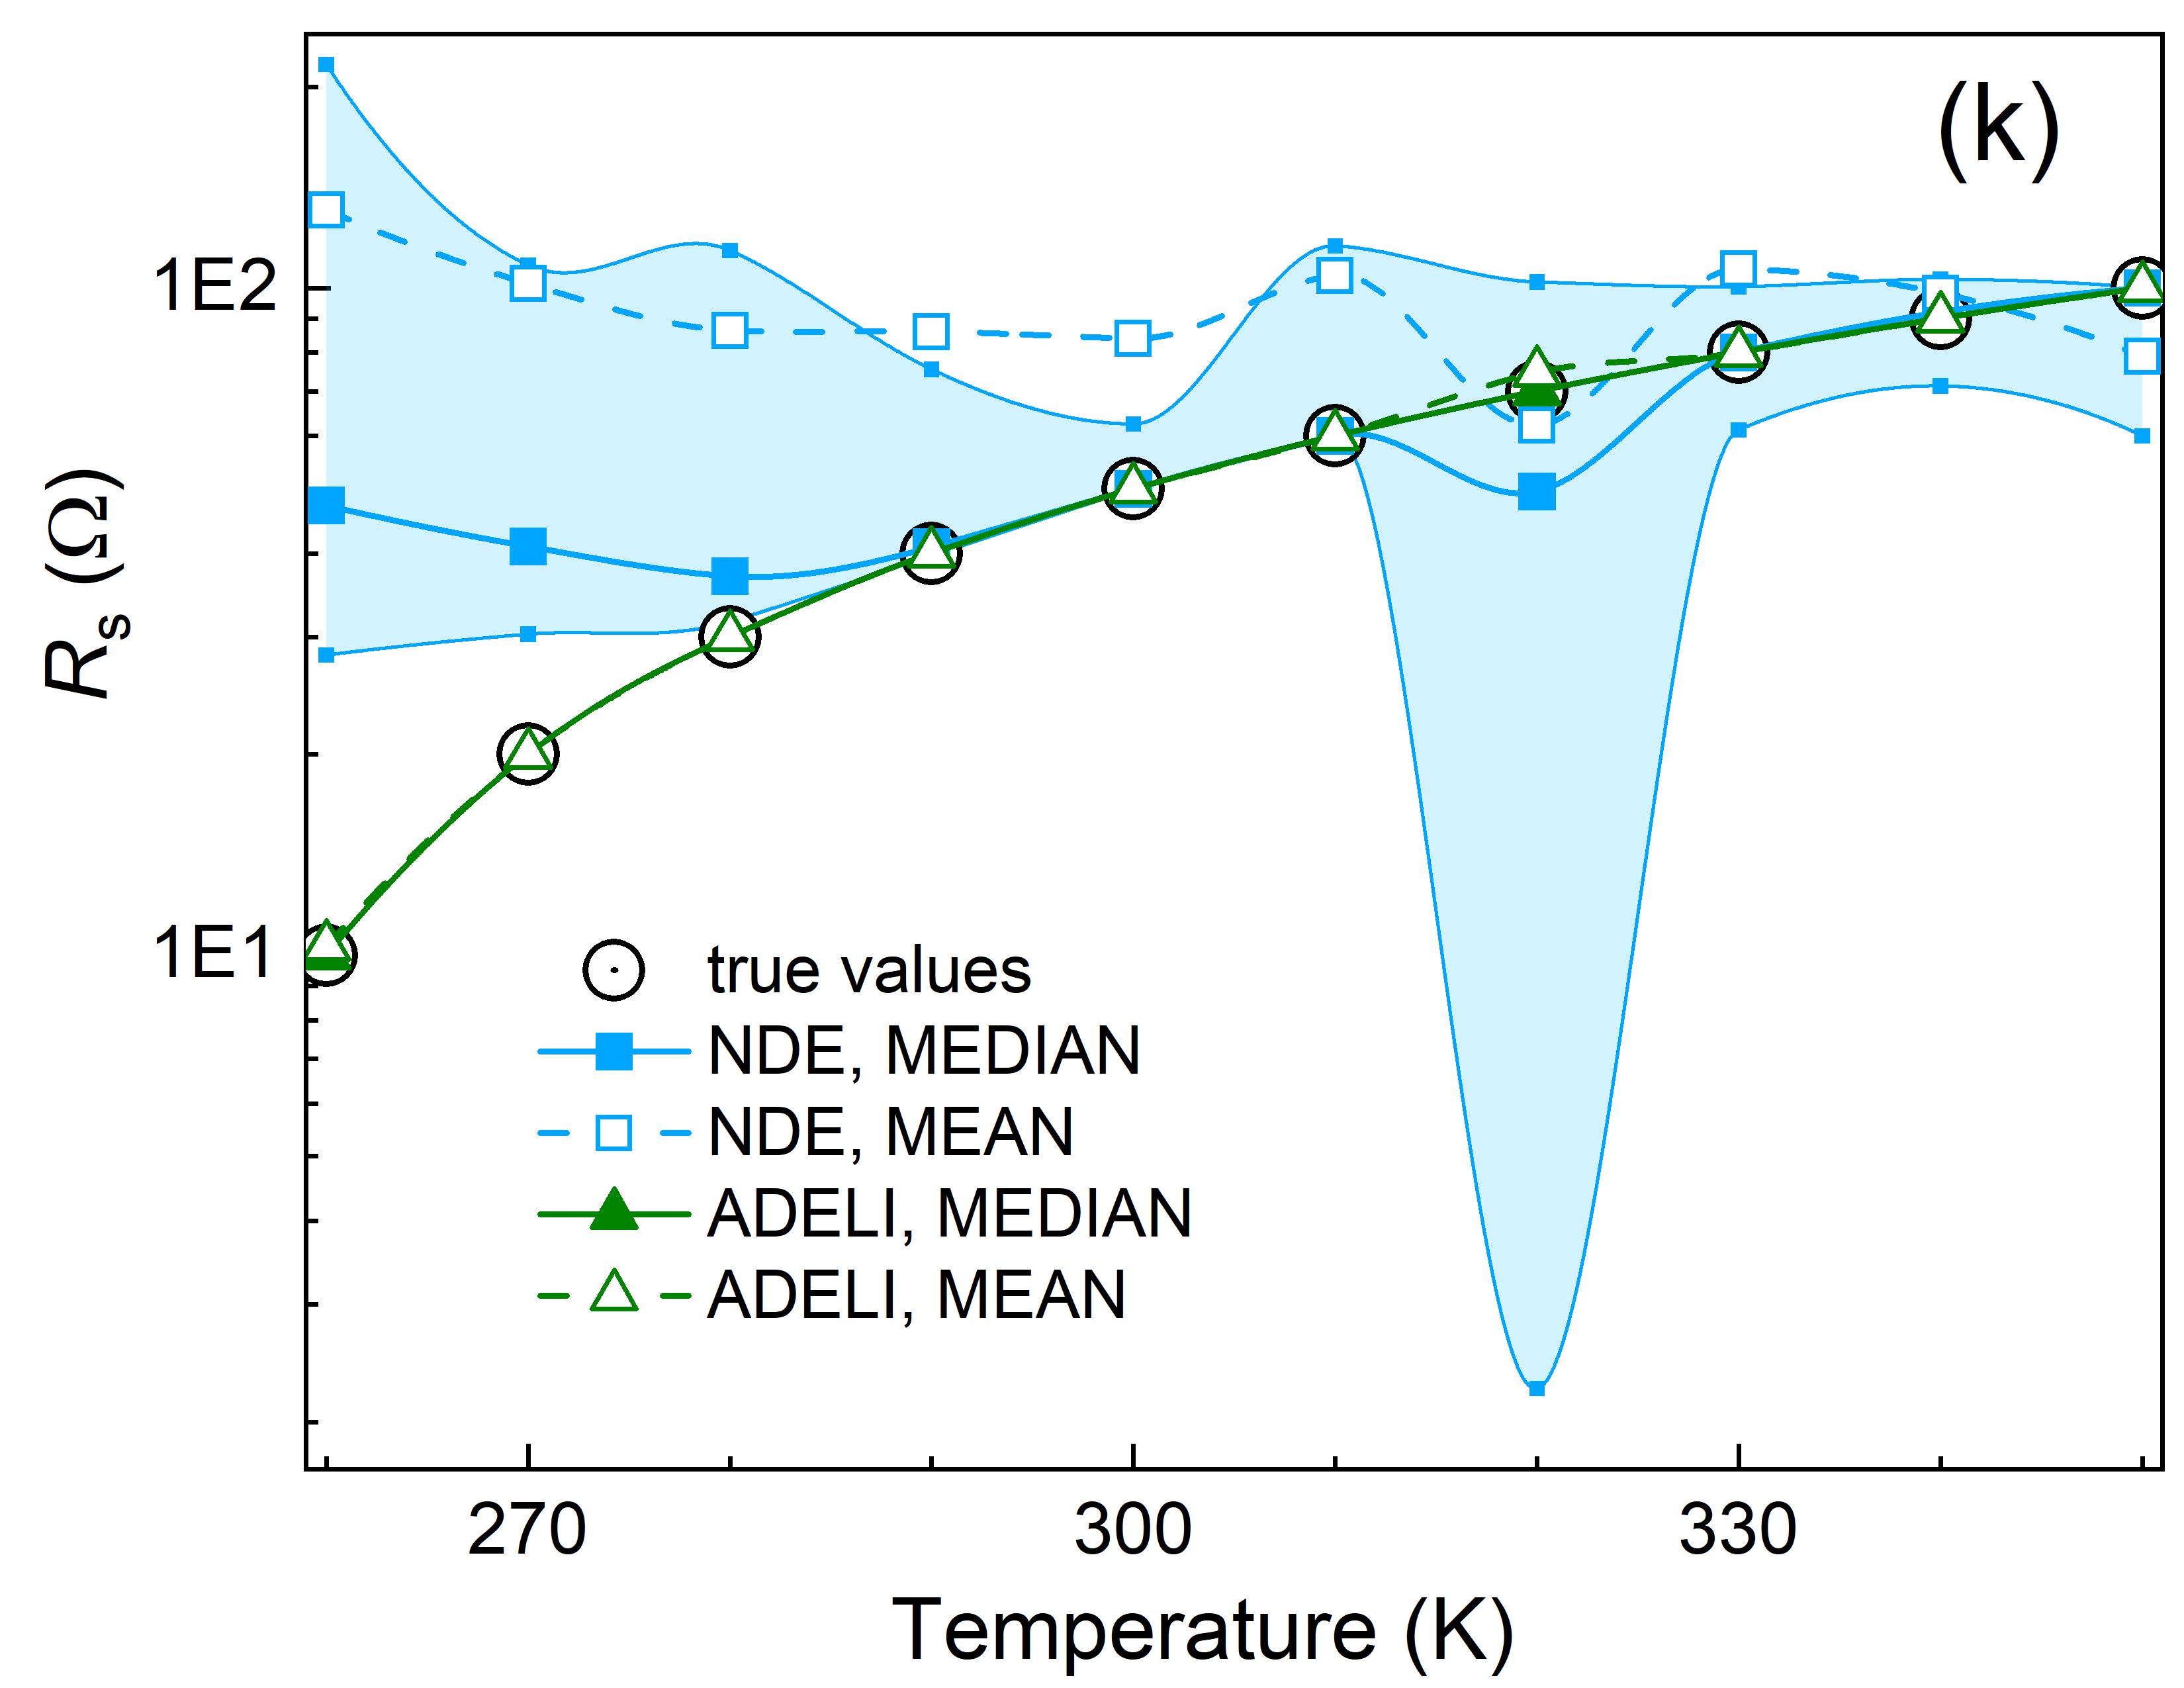
\includegraphics[width=.32\textwidth]{AfigK}
        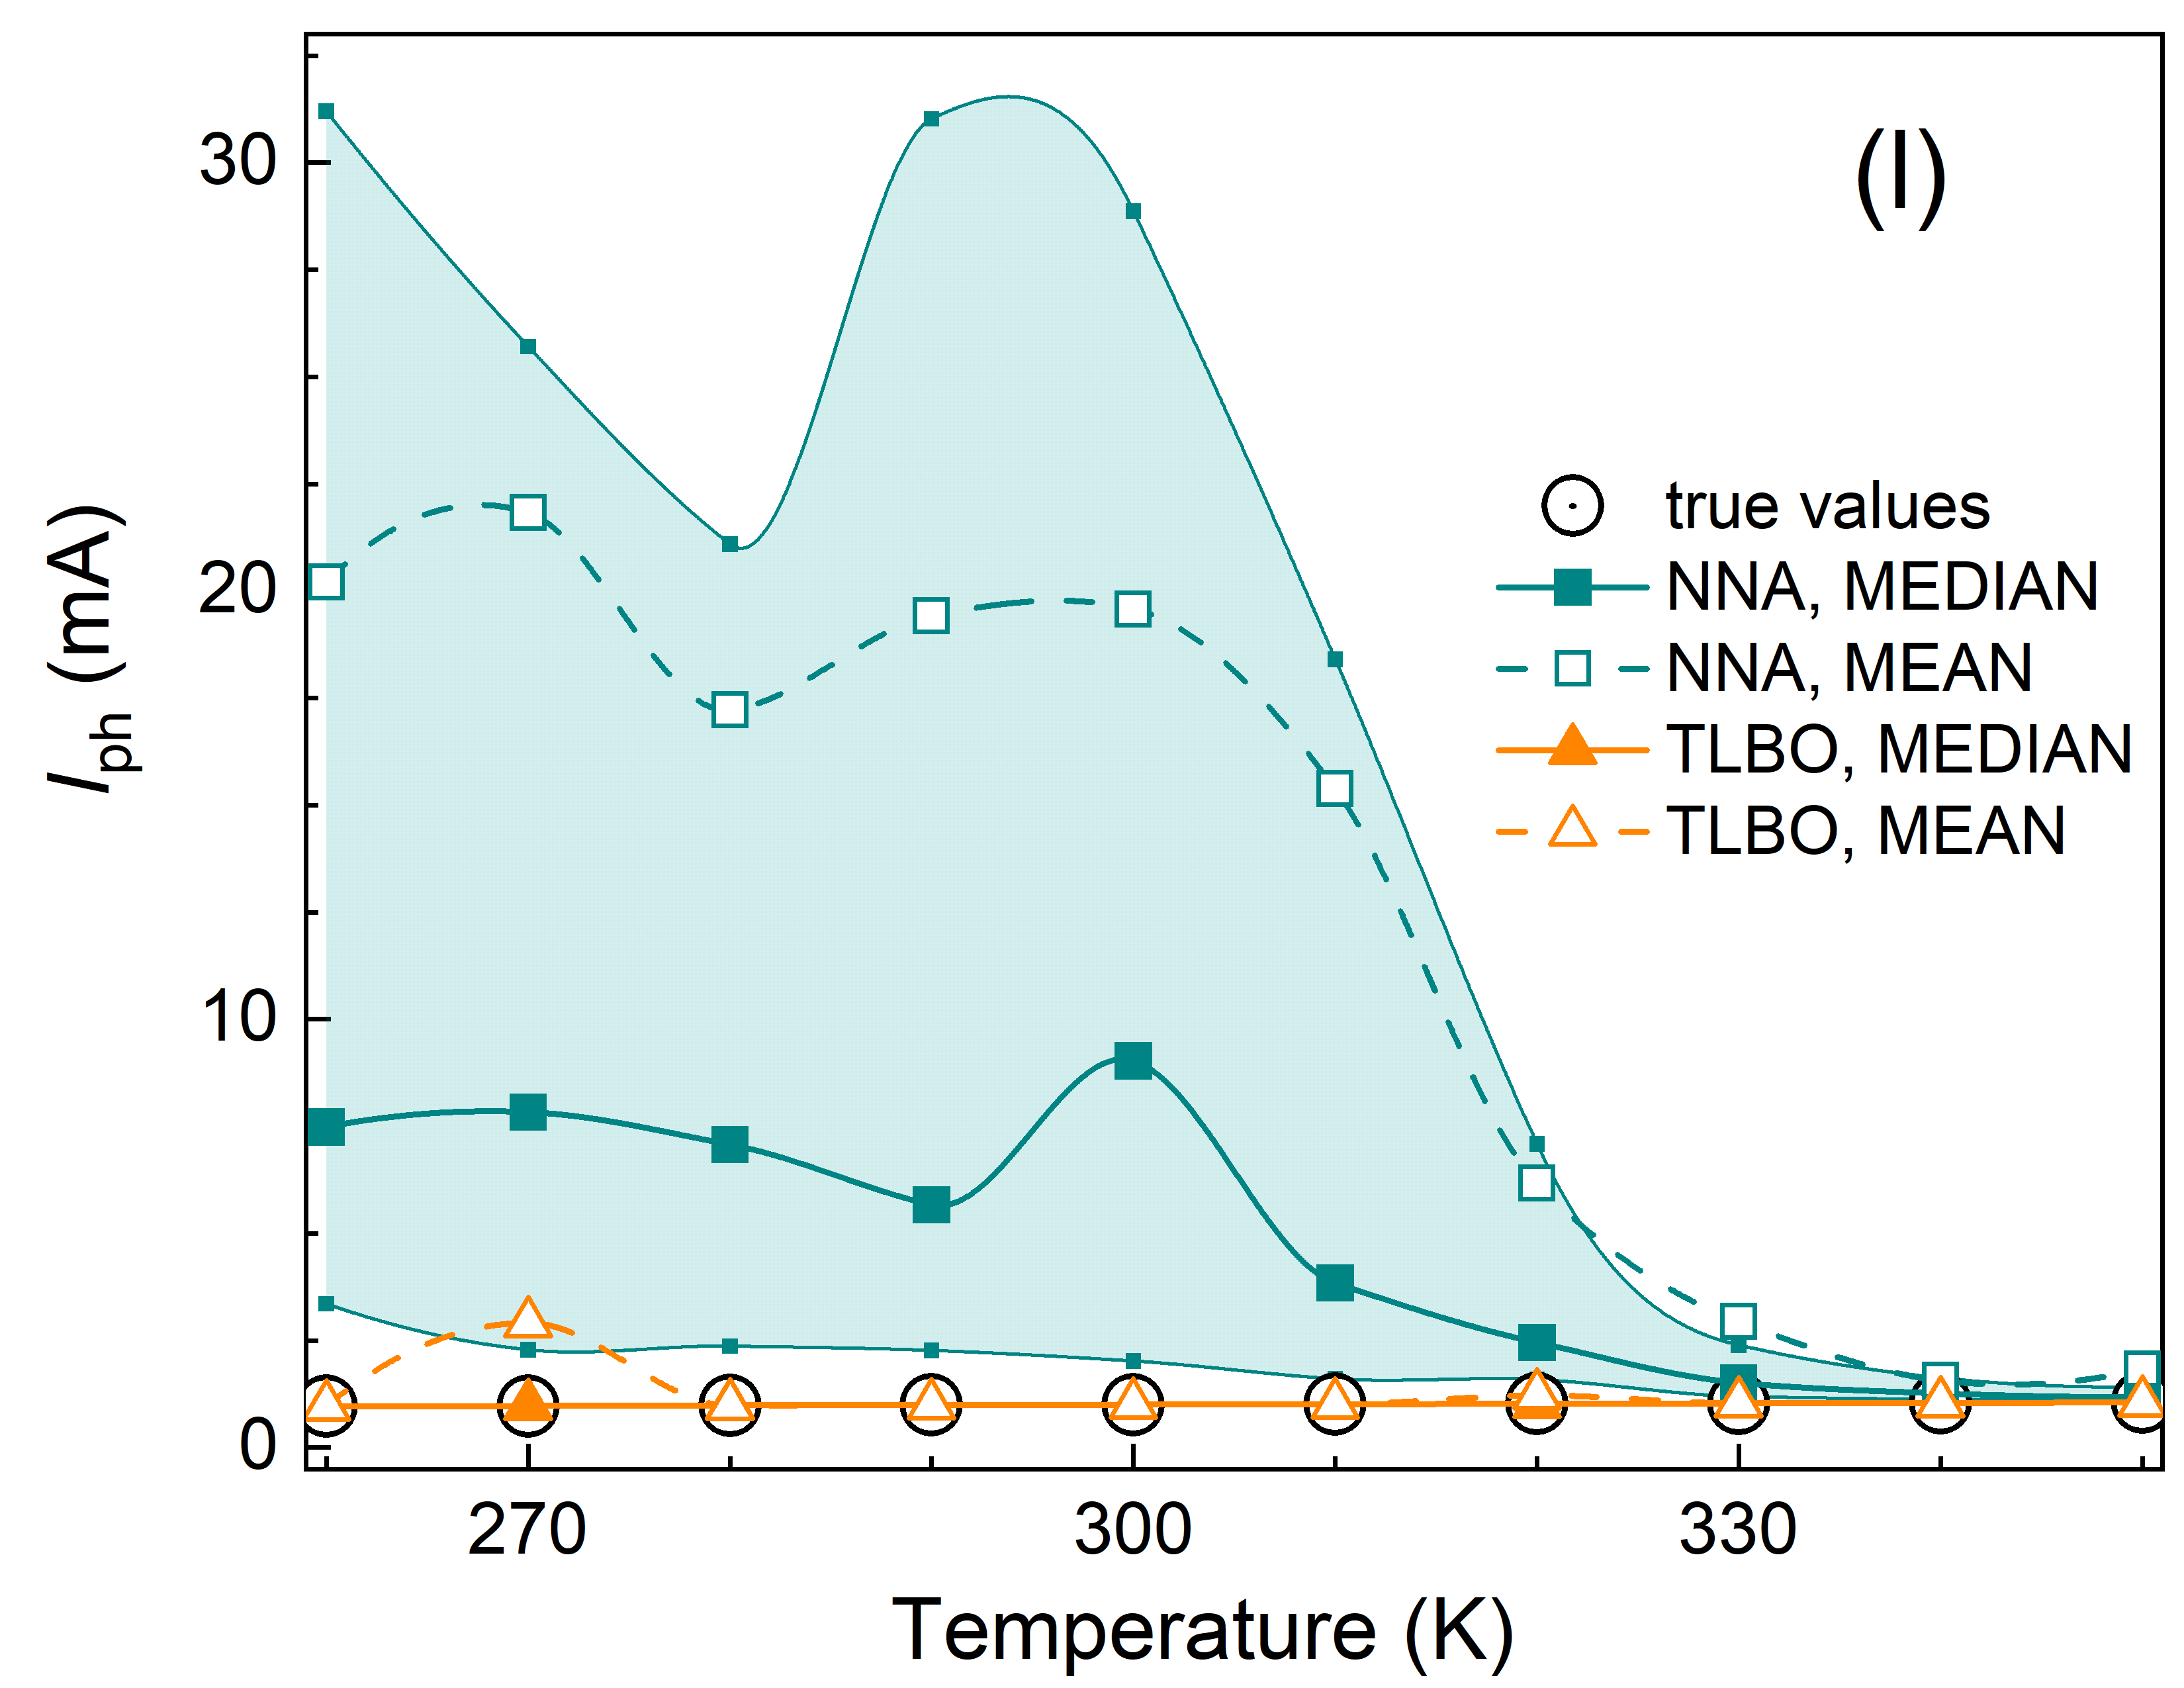
\includegraphics[width=.32\textwidth]{AfigL}
		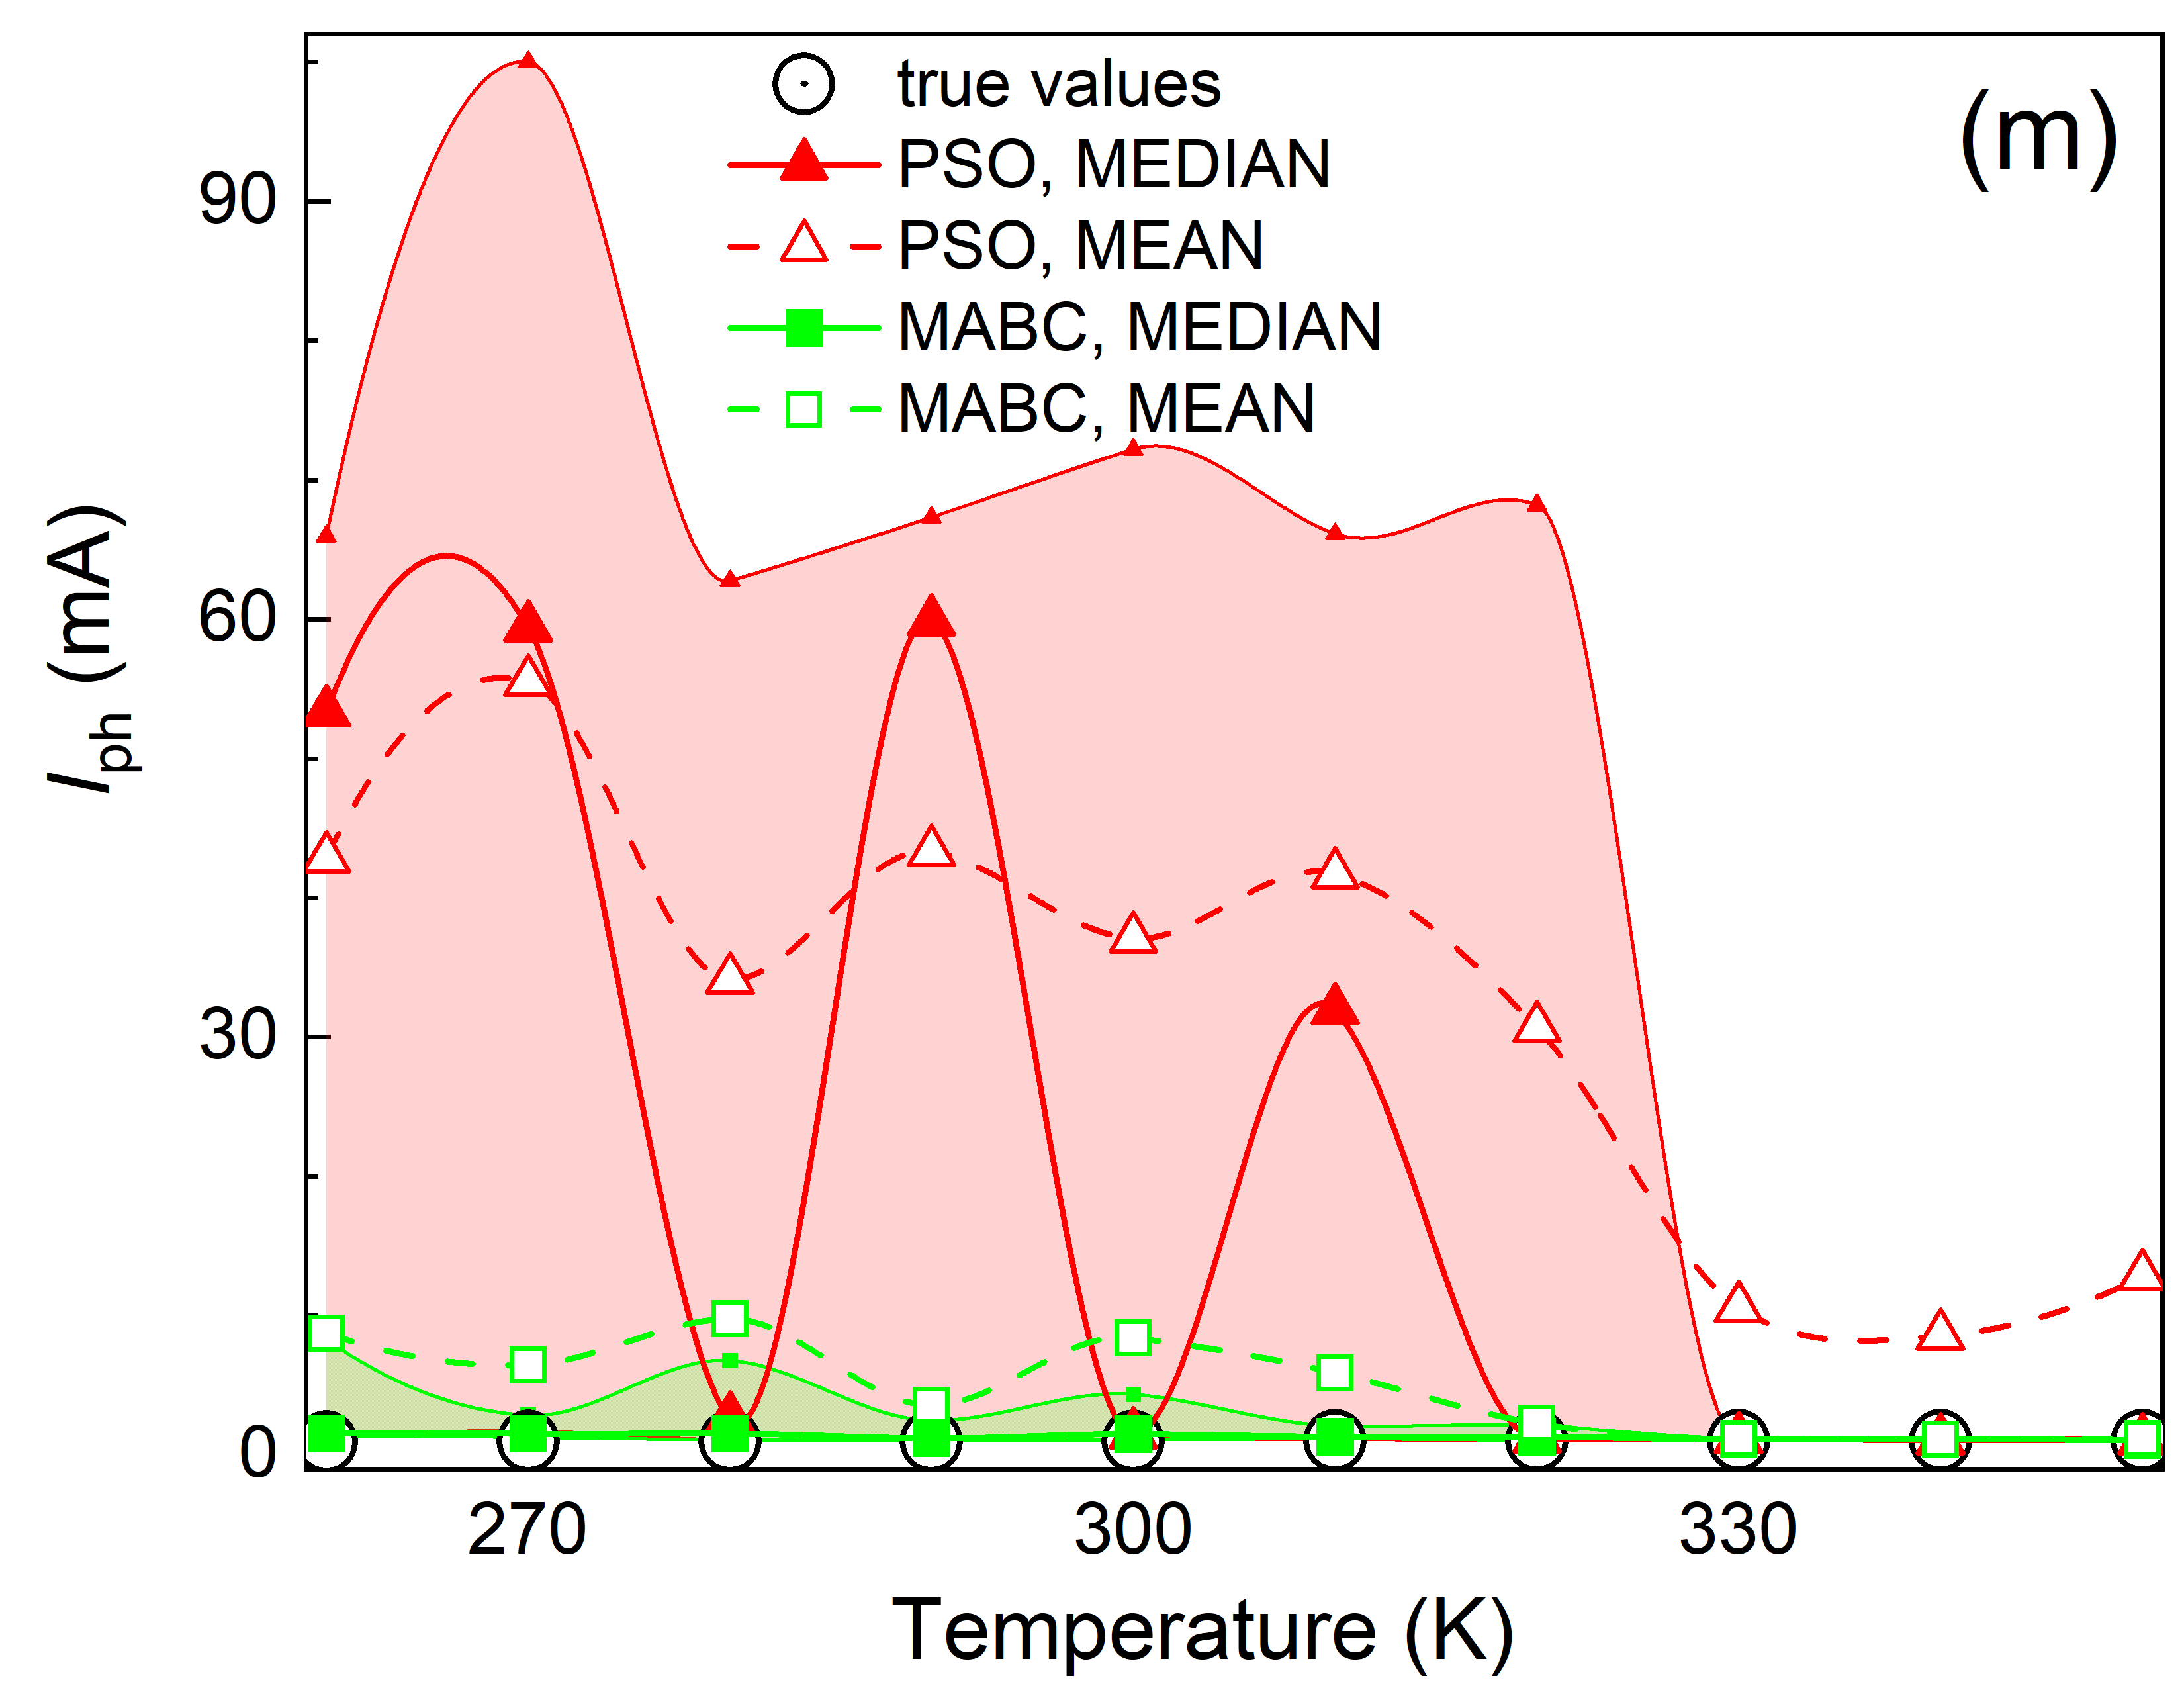
\includegraphics[width=.32\textwidth]{AfigM}
        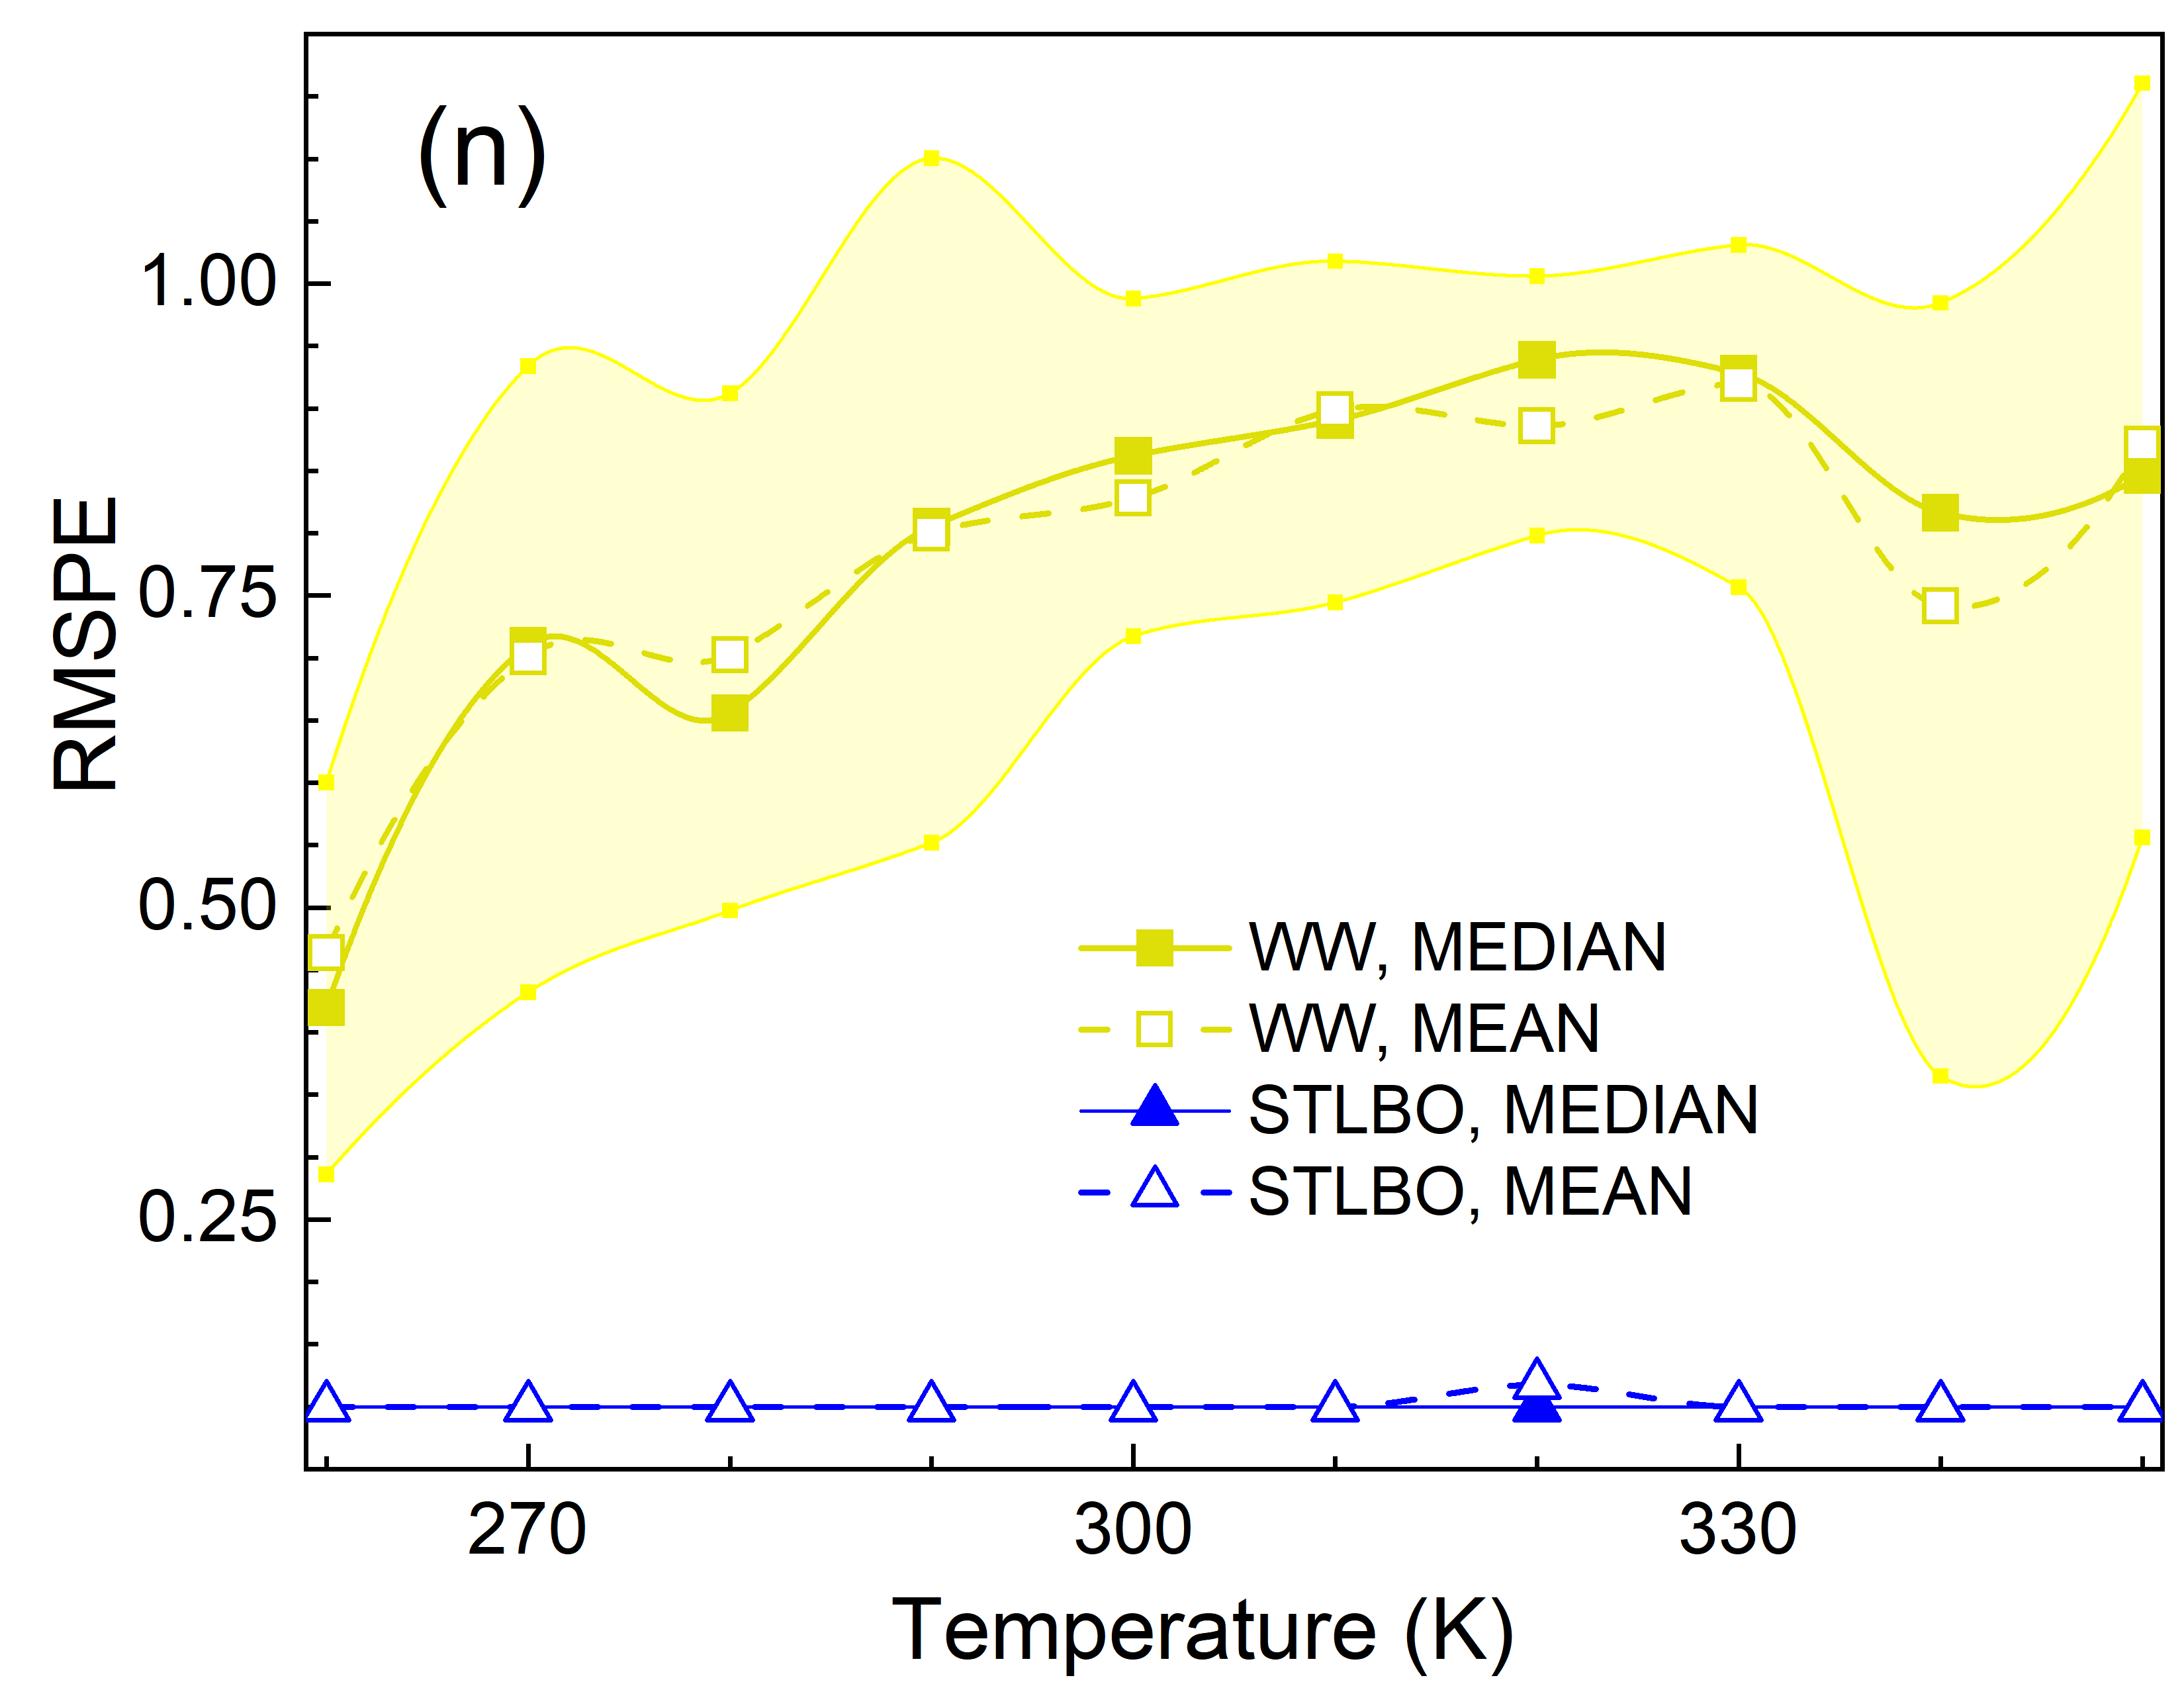
\includegraphics[width=.32\textwidth]{AfigN}
        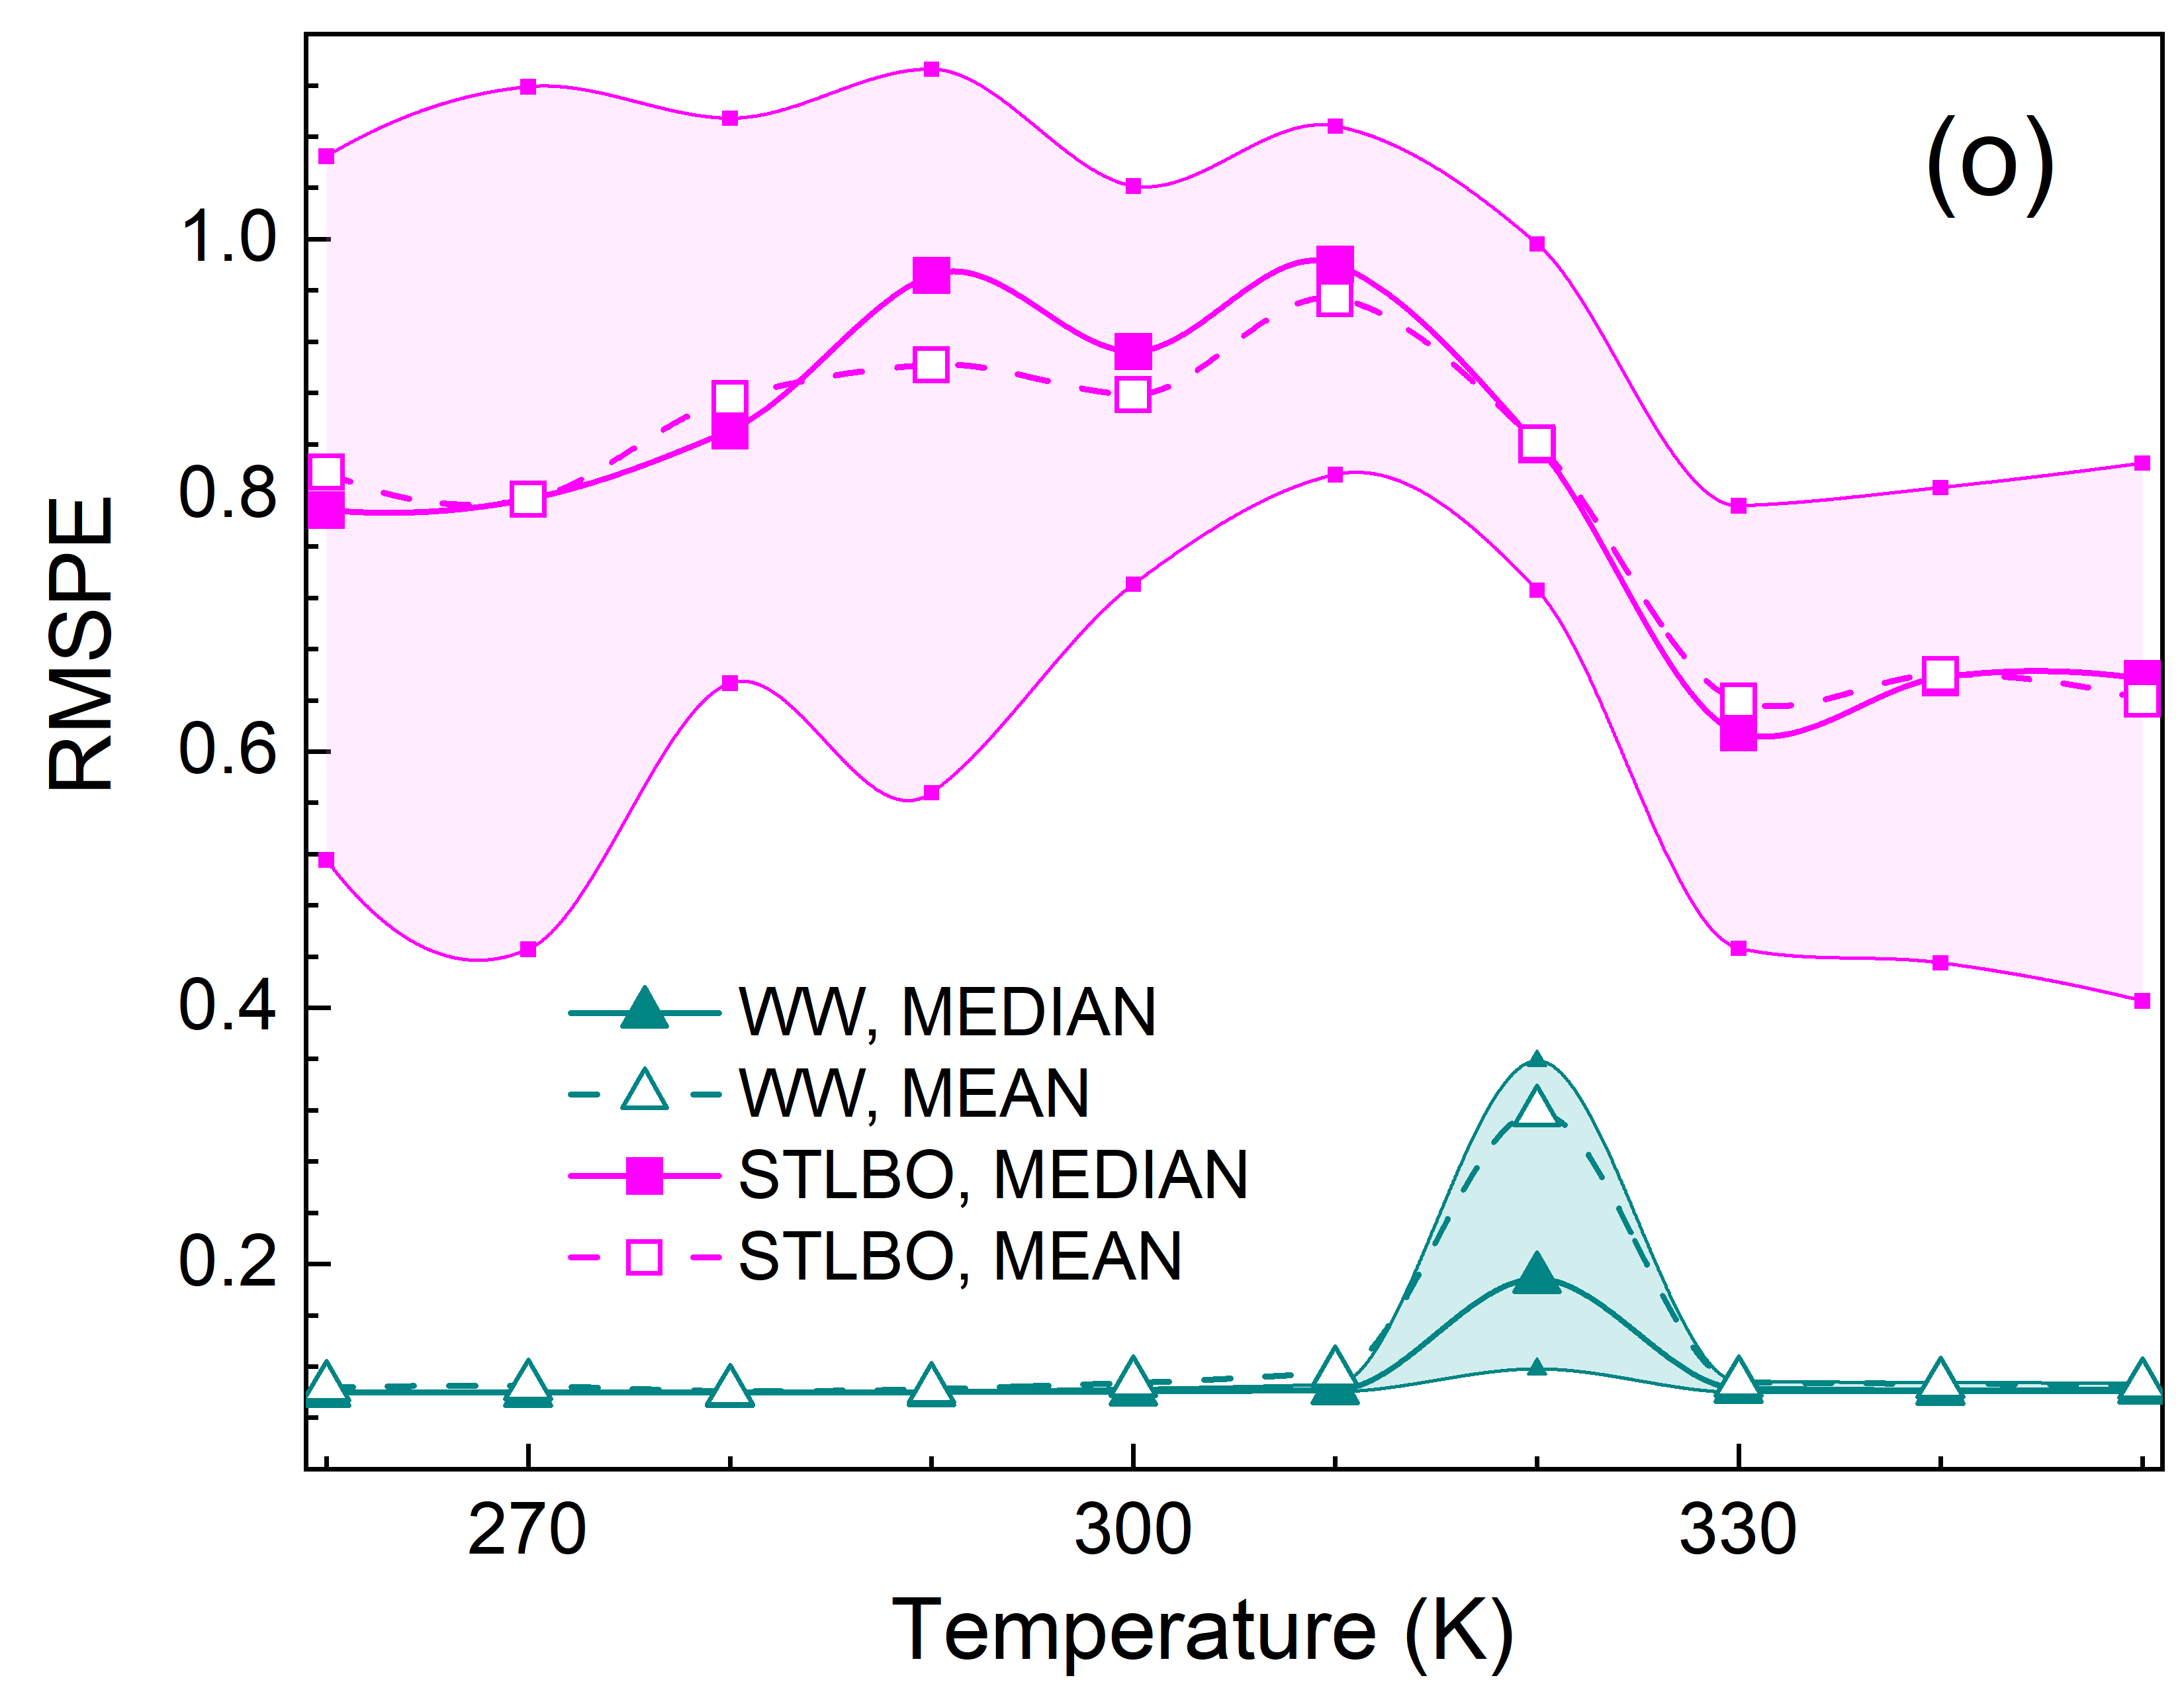
\includegraphics[width=.32\textwidth]{AfigO}
	  \caption{Dependences of the $I_{01}$ (a, b), $n_1$ (c), $R_\mathrm{p1}$ (d), $I_{02}$ (e, f),
               $n_2$ (g, h), $R_\mathrm{p2}$ (i, j), $R_\mathrm{s}$ (k), $I_\mathrm{ph}$ (l, m), and RMSPE (n, o)
               estimation by different algorithm on the synthesis temperature.
               The IV-set is used.
               The circles represent the values, which have been used in IV curve simulations,
               the filled marks represent the median values, and the empty marks represent the mean values.
               The colored regions correspond to the IQR.
               The lines only serve as guide to the eye.
               }\label{figTDepIVset}
\end{figure*}

Fig.~\ref{figSetIV} shows several typical fitting results of a set of synthetic IV curves
simulated according to the opposed two-diode model using the parameter values described in Sec.~\ref{SetIV}.
A more comprehensive and enhanced version, including the fitting results obtained using each algorithm,
is provided in the supplementary materials (figure S4).
Similar to the single--IV case,
the algorithms EBLSHADE, ADELI, NDE, IJAYA, TLBO, and STLBO show
the highest agreement between the fitting curves and the points of synthesized current-voltage curves.
Fig.~\ref{figTDepIVset} represents a portion of the results obtained from evaluating solar cell parameters using various algorithms,
along with the corresponding RMSPE data.
The supplementary material provides the dependencies of all parameters on synthesis temperature
as determined by all the algorithms --- see figures~S5-S13.
The results in terms of MEAN, MEDIAN, STD, and IQR are tabulated as well (table~S154 in the supplementary material).

It should be noted that in several cases, the accuracy of parameter estimation depends on temperature, even for constant parameters.
For instance, as the temperature increases, the errors in determining $R_\mathrm{p1}$ by NDE, MABC, GOTLBO, IJAYA, ISCA, and WW decrease.
However, under the same conditions, the estimation quality of $I_{01}$ using DE, ISCA, and WW worsens.
These results indicate that the accuracy of parameter estimation depends not only on the parameter value itself but also on its ratio with other parameters.
A comprehensive investigation into the specific dependencies of parameter estimation accuracy for each algorithm has not been conducted.
This study aimed to determine the best algorithms rather than elucidate the peculiarities of their application in the context of opposed the two-diode model.

\begin{table*}[<options>]
\caption{The results of Wilcoxon signed-rank test with a level of significance $\alpha = 0.05$ in the IV-set case.
         The ``+'' indicated that the null hypothesis was rejected, and the control algorithm (in the row) performed better
         then the comparison algorithm (in the column).
         The ``0'' indicates to rejection of the hypothesis about outperforming the control algorithm.
         }\label{tblWilIVset}
\begin{tabular*}{\tblwidth}{@{}LCCCCCCCCCCCCCCC@{}}
\toprule
Control & \multicolumn{14}{C}{Comparison algorithm}&Total \\
algorithm  &DE&EBLSHADE&ADELI&NDE&MABC&TLBO&GOTLBO&STLBO&PSO&IJAYA&ISCA&NNA&CWOA&WW&$(+/=/-)$\\ % Table header row
\midrule
DE&$\blacksquare$&0&0&0&+&0&+&0&+&0&+&+&+&+&7/0/6\\
EBLSHADE&+&$\blacksquare$&0&+&+&0&+&0&+&+&+&+&+&+&10/0/3\\
ADELI&+&+&$\blacksquare$&+&+&+&+&+&+&+&+&+&+&+&13/0/0\\
NDE&+&0&0&$\blacksquare$&+&0&+&0&+&+&+&+&+&+&9/0/4\\
MABC&0&0&0&0&$\blacksquare$&0&+&0&+&0&+&+&+&+&6/0/7\\
TLBO&+&+&0&+&+&$\blacksquare$&+&0&+&+&+&+&+&+&11/1/1\\
GOTLBO&0&0&0&0&0&0&$\blacksquare$&0&+&0&+&+&+&+&5/0/8\\
STLBO&+&+&0&+&+&0&+&$\blacksquare$&+&+&+&+&+&+&11/1/1\\
PSO&0&0&0&0&0&0&0&0&$\blacksquare$&0&0&0&0&0&0/4/9\\
IJAYA&+&0&0&0&+&0&+&0&+&$\blacksquare$&+&+&+&+&8/0/5\\
ISCA&0&0&0&0&0&0&0&0&0&0&$\blacksquare$&0&0&0&0/3/10\\
NNA&0&0&0&0&0&0&0&0&0&0&0&$\blacksquare$&0&0&0/3/10\\
CWOA&0&0&0&0&0&0&0&0&0&0&0&0&$\blacksquare$&0&0/4/9\\
WW&0&0&0&0&0&0&0&0&0&0&0&+&0&$\blacksquare$&1/3/9\\
\bottomrule
\end{tabular*}
\end{table*}

\begin{figure}[]
	\centering
		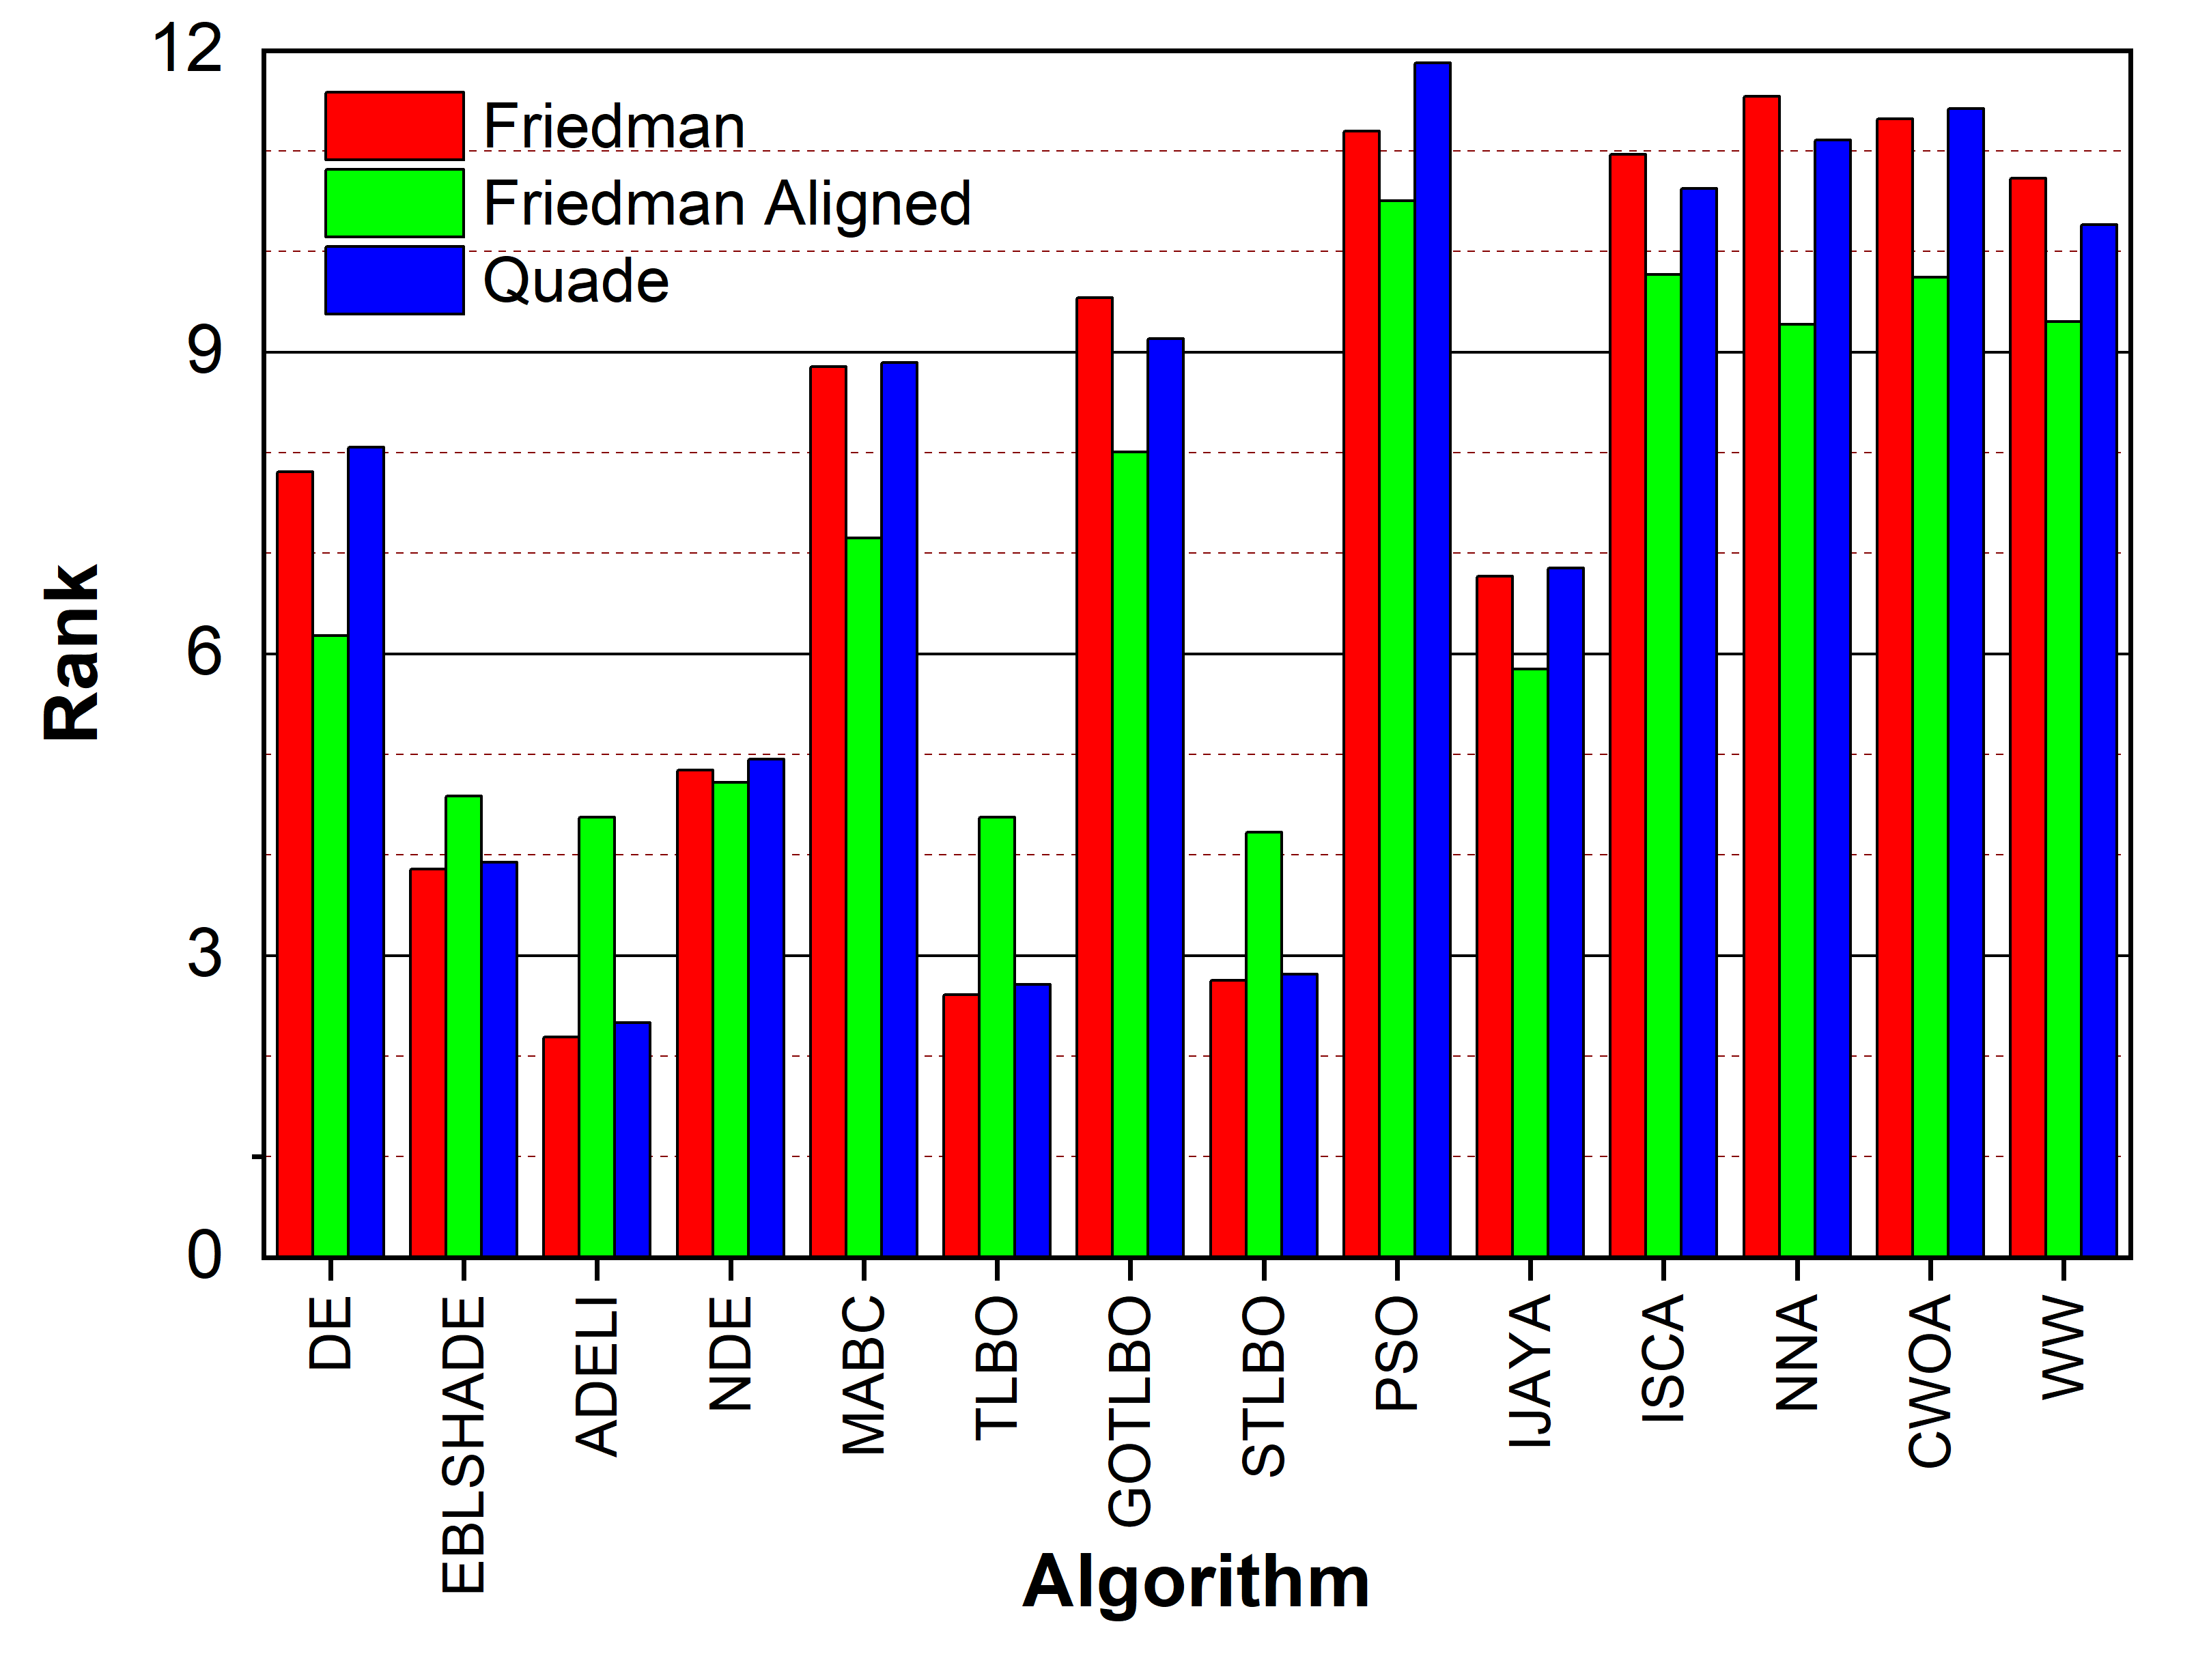
\includegraphics[width=1.0\columnwidth]{FigRankT}
	  \caption{Ranking of the algorithms according to Friedman, Friedman Aligned, and Quade tests in the IV-set case.}\label{figRankIVset}
\end{figure}

The presented data display several characteristics that were also observed in the single-IV case.
For instance, the error in parameters estimating by mean values is higher compared to that of median values in the majority of cases.
Exceptions are observed at some temperatures only when evaluating $I_{01}$ using IJAYA,
$n_1$ using IJAYA and DE,
$R_\mathrm{p1}$ using DE and MABC,
and $R_s$ using DE and WW.
However, for high-precision algorithms, the deviation of MEDIAN from the true value does not exceed the deviation of MEAN.
Additionally, these algorithms exhibit small IQR values that do not exceed STD.
Similar to the previous case, small RMSPE values do not always indicate high accuracy in determining the parameters of a solar cell.

At the same time, the number of algorithms exhibiting minimal errors has decreased.
Significant deviations from true values are observed for median values
of $I_{01}$, $n_{1}$, $R_\mathrm{p1}$, $n_2$, $R_s$, and $I_\mathrm{ph}$ evaluated by EBLSHADE at various temperatures,
as well as for median values of diode D1 characteristics and series resistor determined using TLBO at 260~K.
Thus, only ADELI and STLBO remain as algorithms without visible errors.
Although this claim of infallibility applies only to median values,
substantial errors are observed for mean values in several cases.
Simultaneously, EBLSHADE, TLBO, IJAYA, and NDE form a group of algorithms with low RMSPE values but imperfect model parameter estimation.

%a comprehensive nonparametric statistical analysis of algorithms efficiency was performed on all parameters collected from all simulated curves.
In the IV--set case, to assess the statistical performance of compared algorithms,
the run time and all $\mathrm{APE}_\mathrm{MEDIAN}$ and $\mathrm{RMSPE}_\mathrm{MEDIAN}$ for each IV curve were taken into account.
This approach is similar to the use of the Comp parameter in the previous subsection;
however, in this scenario, $N_\mathrm{pr}=81$ is employed:
\begin{equation*}
N_\mathrm{pr}= 10\,T_\mathrm{values}\times(8\,\mathrm{APE}_\mathrm{MEDIAN}+1\,\mathrm{RMSPE}_\mathrm{MEDIAN})+1\,t_\mathrm{run}\,.
\end{equation*}
%10 temperature values $\times(\mathrm{APE}_\mathrm{MEDIAN}+1\mathrm{RMSPE}_\mathrm{MEDIAN})+1t_\mathrm{run}$.
Therefore, such an approach is well-suited for nonparametric statistical analysis of $k=14$ meta-heuristic algorithms.
Certainly, at first sight, it would be interesting to consider incorporating an additional 80 values of the interquartile range into the dataset.
This approach could provide consideration into the stability of algorithm performance as well.
However, it is known \cite{Derrac2011} that for multiple comparisons, a value of $N_\mathrm{pr}\geq 8\cdot k=112$ could be too high, obtaining
no significant comparisons as a result.

Table~\ref{tblWilIVset}  gives the statistical results produced by the Wilcoxon sign--rank test.
As the table states, ADELI outperforms all other algorithms with a level of significance $\alpha = 0.05$.
STLBO and TLBO show an improvement over
DE, EBLSHADE, NDE, MABC, GOTLBO, PSO, IJAYA, ISCA, NNA, CWOA, and WW.
The counts of statistical significant cases $(+/=/-)$ are presented in the last row of Table~\ref{tblWilIVset}.
It can be seen than PSO, ISCA, NNA, and CWOA did not outperform any of the algorithms,
whereas WW statistically significantly improved over  NNA only.
Therefore, although these algorithms have promising run times,
they are not recommended for parameter estimation of a solar cell based on the opposed two-diode model.

The $p$-values required to test the null hypothesis,
computed using the Friedman, Friedman Aligned, Quade tests, and the Iman--Davenport extension,
can be found in table~S2 of the supplementary materials.
None of these values exceeds $2.3\cdot10^{-6}$, thereby rejecting the hypothesis of equivalent medians in all tests.

Ranks achieved by the Friedman, Friedman Aligned, and Quade tests are shown in Fig.~\ref{figRankIVset} and table~S3 in the supplementary material.
As per the given results, ADELI has been placed at first rank by Friedman and Quade tests,
and STLBO has ranked first by the Friedman Aligned test.
TLBO has been recorded the as second-best algorithm by all three tests.
Furthermore, PSO was recognized as the worst-performing algorithm by the tests' unanimous decision.


%\begin{table*}[<options>]
%\caption{Adjusted $p$-values for Friedman, Friedman Aligned, and Quade tests in IV--set case.
% STLBO is the control algorithm.}\label{tbl1NSTLBO}
%\begin{tabular*}{\tblwidth}{@{}LLCCCC@{}}
%\toprule
%\multirow{2}{*}{Algorithm}& \multirow{2}{*}{Test}& \multicolumn{4}{C}{post-hoc procedure} \\
%  & &Finner & Holm & Hochberg &Holland\\ % Table header row
%\midrule
%GOTLBO&	Friedman&<1E-13&<1E-13&<1E-13&<1E-13\\
%&Friedman Aligned&1.35278E-10&5.09895E-10&5.09895E-10&5.09895E-10\\
%&Quade&1.11445E-03&4.11614E-03&4.11614E-03&4.10873E-03\\
%PSO&Friedman&<1E-13&<1E-13&<1E-13&<1E-13\\
%&Friedman Aligned&<1E-13&<1E-13&<1E-13&<1E-13\\
%&Quade&8.22938E-06&8.22941E-06&8.22941E-06&8.22938E-06\\
%NNA&Friedman&<1E-13&<1E-13&<1E-13&<1E-13\\
%&Friedman Aligned&<1E-13&<1E-13&<1E-13&<1E-13\\
%&Quade&2.21284E-05&5.61727E-05&5.61727E-05&5.61713E-05\\
%CWOA&Friedman&<1E-13&<1E-13&<1E-13&<1E-13\\
%&Friedman Aligned&<1E-13&<1E-13&<1E-13&<1E-13\\
%&Quade&1.48311E-05&2.73807E-05&2.73807E-05&2.73803E-05\\
%DE&Friedman&2.32081E-13&8.03357E-13&8.03357E-13&8.03357E-13\\
%&Friedman Aligned&1.74950E-09&6.45968E-09&6.45968E-09&6.45968E-09\\
%&Quade&6.44257E-03&2.38175E-02&2.38175E-02&2.35824E-02\\
%IJAYA&Friedman&2.17645E-10&8.03613E-10&8.03613E-10&8.03613E-10\\
%&Friedman Aligned&3.63299E-09&1.25757E-08&1.25757E-08&1.25757E-08\\
%&Quade&3.78757E-02&1.31885E-01&1.31885E-01&1.25109E-01\\
%MABC&Friedman&1.75608E-09&6.61909E-09&6.61909E-09&6.61909E-09\\
%&Friedman Aligned&<1E-13&<1E-13&<1E-13&<1E-13\\
%&Quade&1.54776E-03&5.83595E-03&5.83595E-03&5.82137E-03\\
%WW&Friedman&7.44635E-09&2.74942E-08&2.74942E-08&2.74942E-08\\
%&Friedman Aligned&<1E-13&<1E-13&<1E-13&<1E-13\\
%&Quade&1.10078E-04&3.81053E-04&3.81053E-04&3.80989E-04\\
%ISCA&Friedman&1.32325E-08&4.58048E-08&4.58048E-08&4.58048E-08\\
%&Friedman Aligned&<1E-13&<1E-13&<1E-13&<1E-13\\
%&Quade&5.64886E-05&1.73815E-04&1.73815E-04&1.73801E-04\\
%NDE&Friedman&9.57698E-04&2.94709E-03&2.94709E-03&2.94383E-03\\
%&Friedman Aligned&2.69373E-03&8.29097E-03&8.29097E-03&8.26522E-03\\
%&Quade&2.98714E-01&9.55486E-01&9.55486E-01&6.64392E-01\\
%EBLSHADE&Friedman&8.62842E-02&2.20533E-01&2.20533E-01&2.04719E-01\\
%&Friedman Aligned&3.10807E-02&7.90881E-02&7.90881E-02&7.70214E-02\\
%&Quade&5.99120E-01&1.0&1.0&9.01765E-01\\
%ADELI&Friedman&1.0&1.0&1.0&1.0\\
%&Friedman Aligned&3.64522E-01&6.83937E-01&3.45600E-01&5.66995E-01\\
%&Quade&1.0&1.0&1.0&1.0\\
%TLBO&Friedman&1.0&1.0&1.0&1.0\\
%&Friedman Aligned&3.64522E-01&6.83937E-01&3.45600E-01&5.66995E-01\\
%&Quade&1.0&1.0&1.0&1.0\\
%\bottomrule
%\end{tabular*}
%\end{table*}




\begin{figure}[]
	\centering
		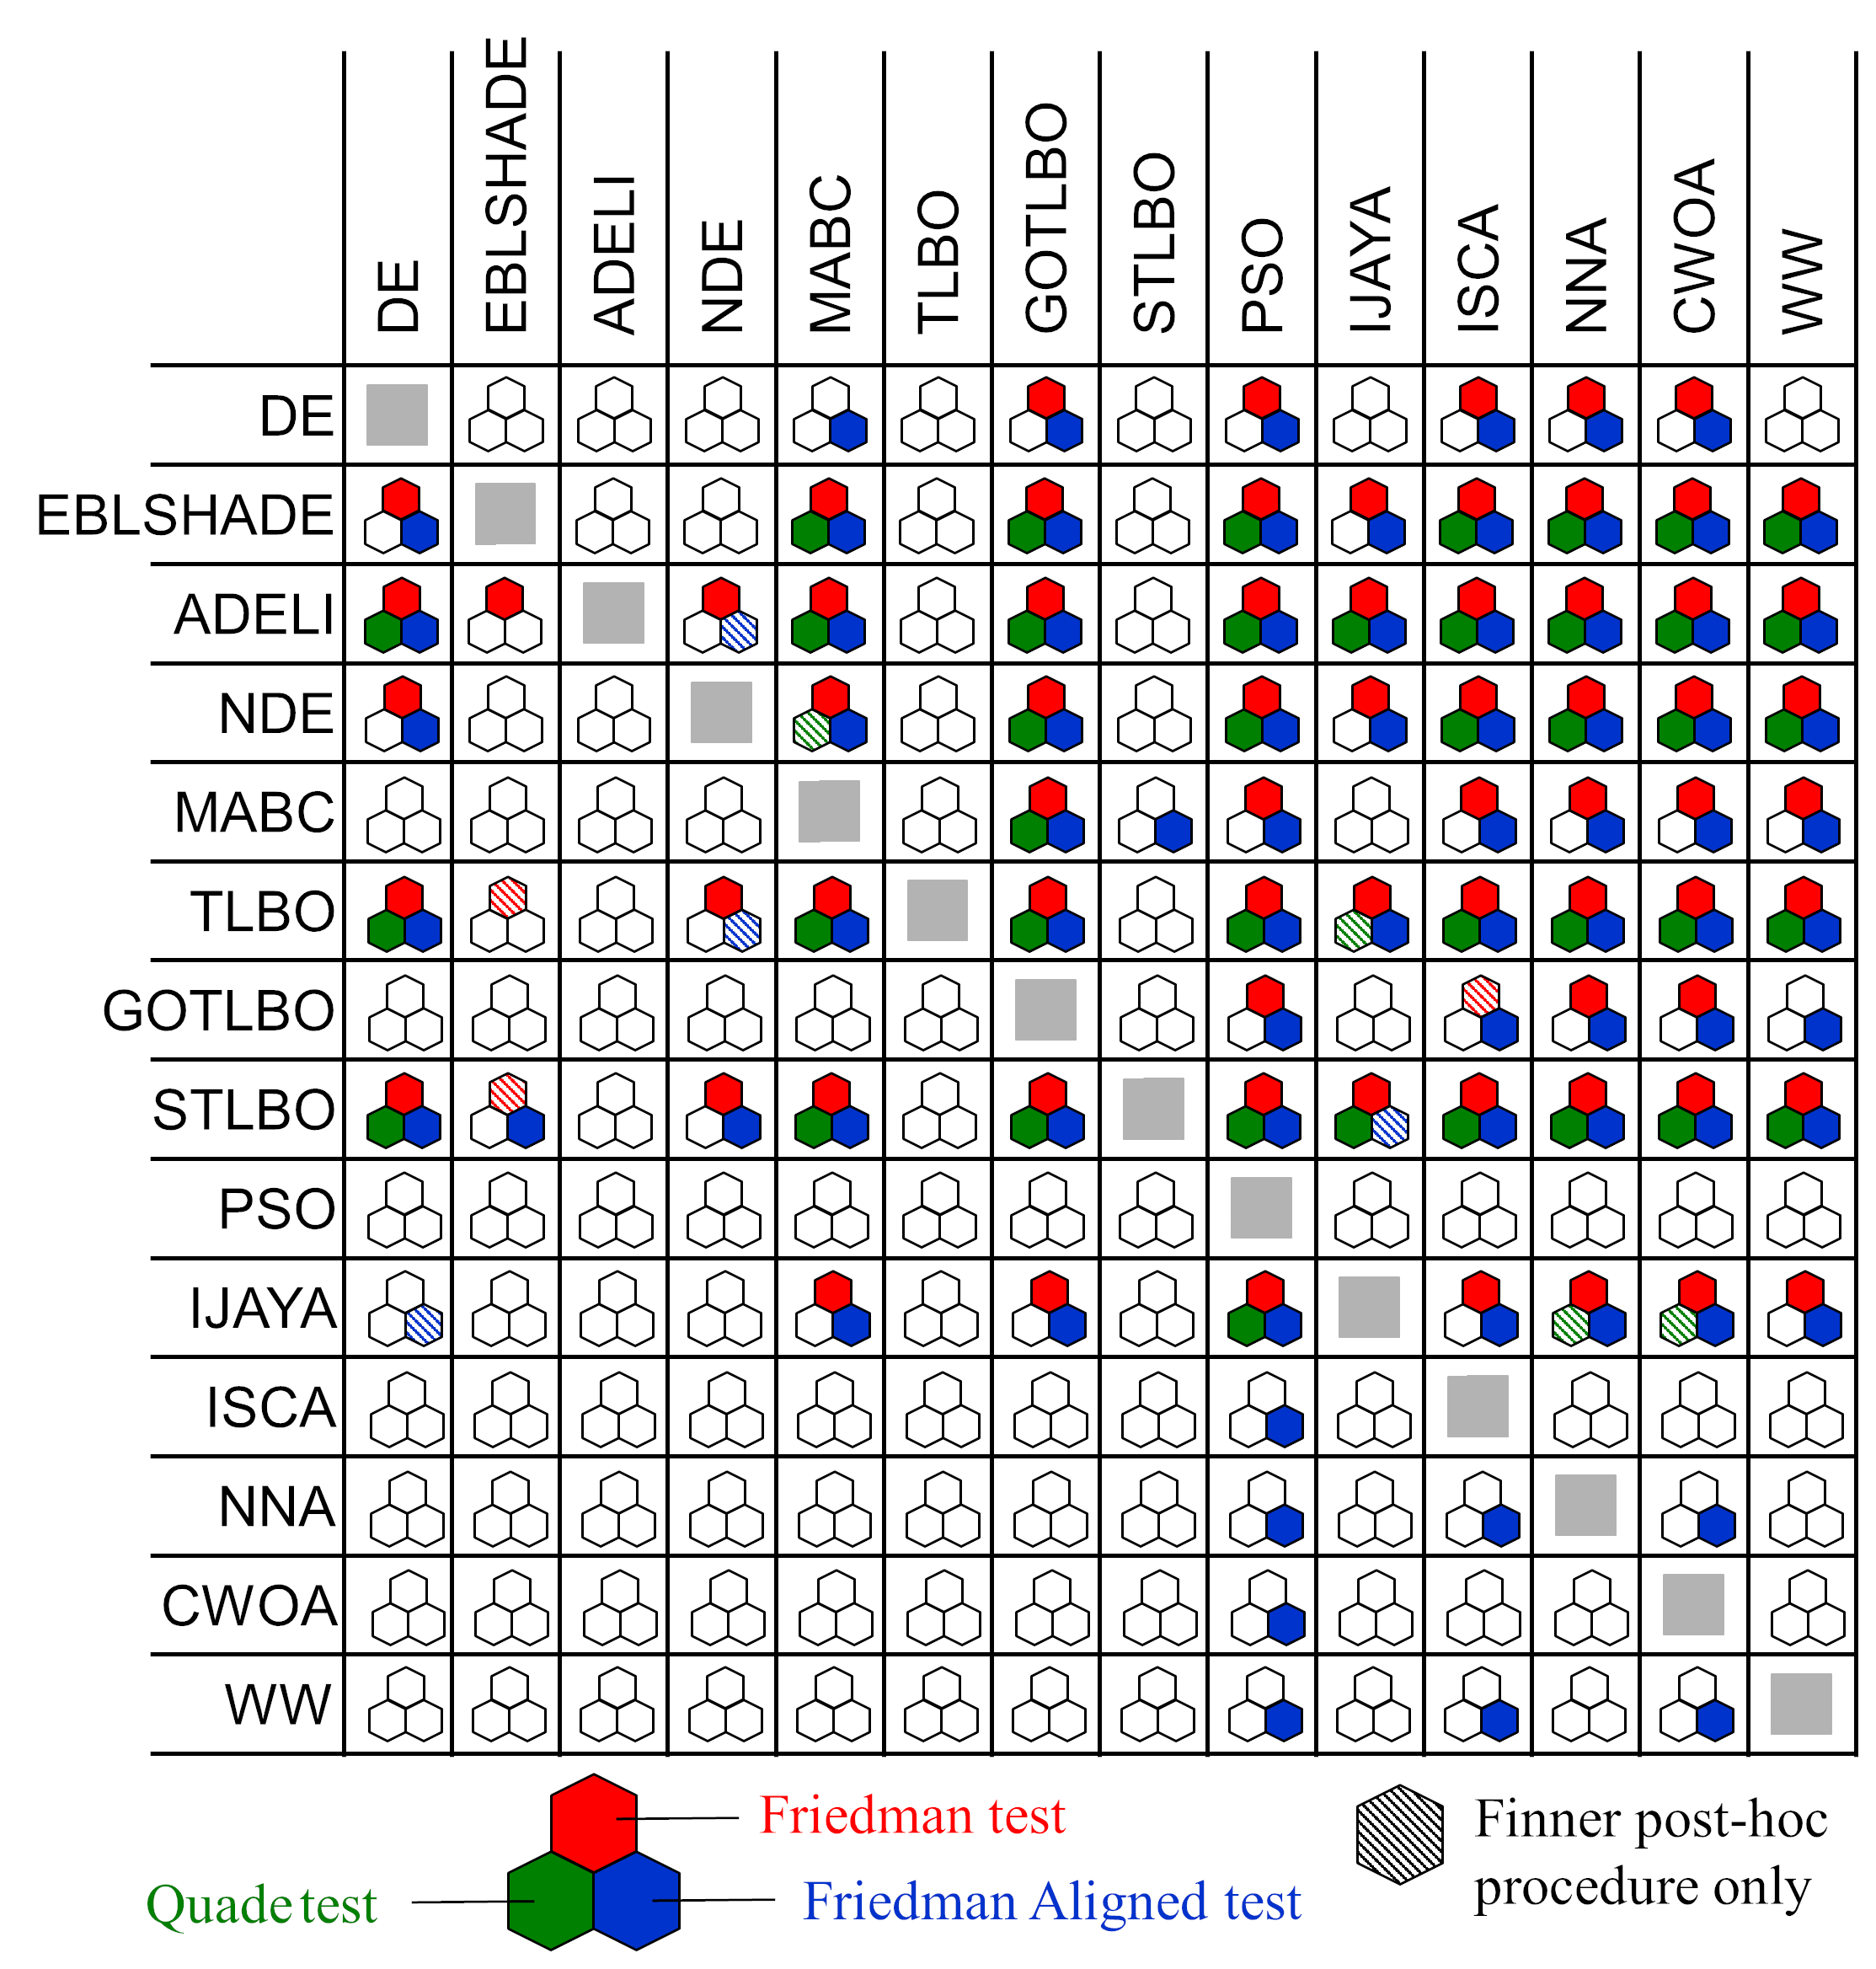
\includegraphics[width=1.0\columnwidth]{N1Tresult}
	  \caption{The results of algorithm $1\times N$ comparisons by Friedman, Friedman Aligned, and Quade tests in the IV-set case.
               The colored hexagon indicates that the adjusted $p$-value,
               which tests the hypothesis that an algorithm in a row outperforms the algorithm in a column,
               is not greater than $p_{cr}=0.1$.
               The solid fill signifies that every post-hoc procedure resulted in $p<p_{cr}$;
               the dashed fill indicates that the Finner post-hoc procedure was the only method that produced this result.
               The correspondence between the color and position of the hexagon to a test
               is shown in a legend at the bottom of the figure.
               }\label{figN1RezIVset}
\end{figure}


\begin{figure}[]
	\centering
		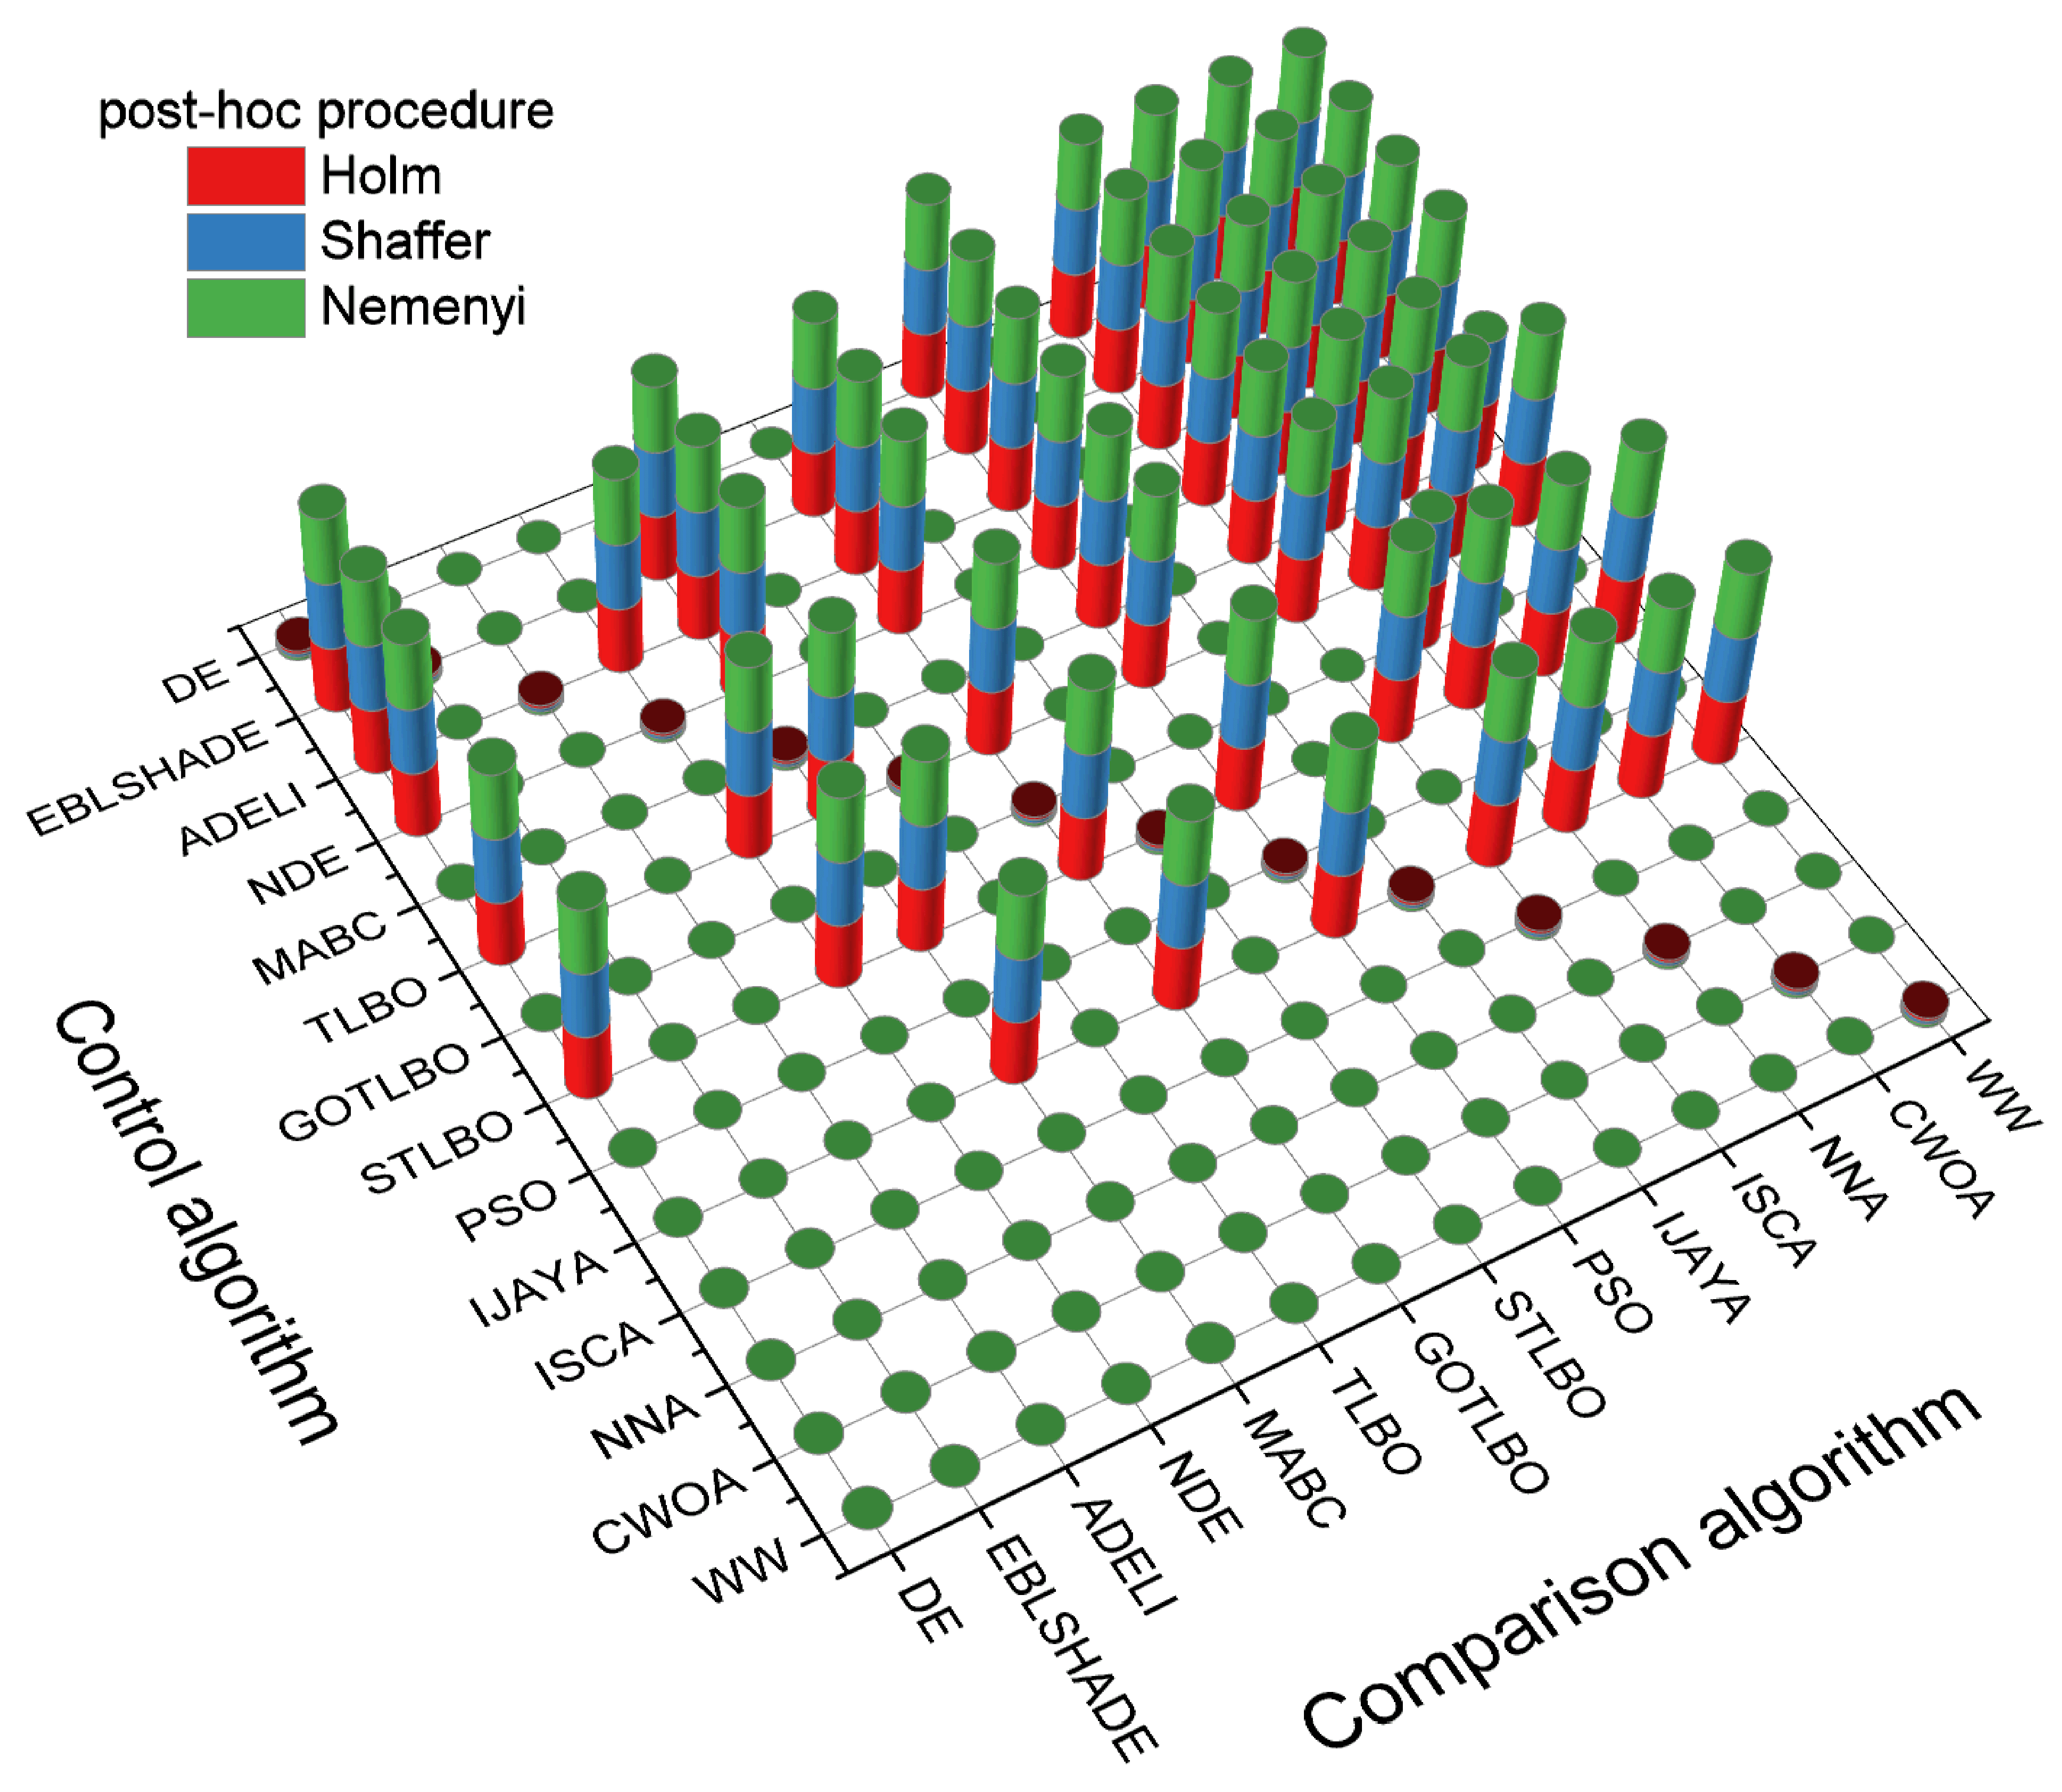
\includegraphics[width=1.0\columnwidth]{NNresult}
	  \caption{The results of multiple comparisons among all algorithms in the IV-set case.
               The colored cylinder indicates that the adjusted p-value,
               which tests the control algorithm outperforms the comparison algorithm,
               is not greater than $p_{cr}=0.1$.
               The correspondence between the color of the cylinder to a post-hoc procedure is shown in the figure's legend.
               }\label{figNNRezIVset}
\end{figure}

\begin{table}[<options>]
\caption{The total count of wins and losses for each algorithm in $1\times N$ and $N\times N$ multiple comparisons using the
all tests and post-hoc procedures in the IV-set case.
The criterion for victory was a adjusted $p$-value less than 0.1.
The best results are bolded.
}\label{tblAllWins}
\begin{tabular*}{\tblwidth}{@{}LCC@{}}
\toprule
\multirow{2}{*}{Algorithm}& \multicolumn{2}{C}{Wins / Loses} \\
  & $1\times N$ comparisons& $N\times N$ comparisons\\ % Table header row
\midrule
DE & 44/53 & 15/15\\
EBLSHADE & 100/6 & 24/\textbf{0} \\
ADELI & 117/\textbf{0} & \textbf{27}/\textbf{0}\\
NDE & 97/18 & 24/9\\
MABC &  44/69 & 14/18\\
TLBO & 111/\textbf{0} & \textbf{27}/\textbf{0}\\
GOTLBO & 25/80 & 2/18\\
STLBO & \textbf{118}/\textbf{0} & \textbf{27}/\textbf{0}\\
PSO & 0/112 & 0/24\\
IJAYA &  63/46 & 21/\textbf{0}\\
ISCA & 4/97 & 0/24\\
NNA & 12/93 & 0/26\\
CWOA & 4/101 & 0/24\\
WW & 12/80 & 0/23\\
\bottomrule
\end{tabular*}
\end{table}




%\begin{table*}[<options>]
%\caption{Adjusted $p$-values for tests for multiple $N\times N$ comparisons among all methods
%         in the IV--set case ($p<p_{lim}$ are only shown).}\label{tblNNpValue}
%\begin{tabular*}{\tblwidth}{@{}LCCC@{}}
%\toprule
%\multirow{2}{*}{Hypothesis}& \multicolumn{3}{C}{post-hoc procedure} \\
%  &Nemenyi & Holm & Shaffer\\ % Table header row
%\midrule
%EBLSHADE versus WW,
%ADELI versus MABC,&&&\\
%ADELI versus PSO,
%ADELI versus ISCA,&&&\\
%ADELI versus NNA,
%ADELI versus CWOA,&&&\\
%ADELI versus WW,
%NDE versus NNA,&&&\\
%TLBO versus GOTLBO,
%TLBO versus PSO,&&&\\
%TLBO versus ISCA,
%TLBO versus NNA,&&&\\
%TLBO versus CWOA,
%STLBO versus GOTLBO, &&&\\
%STLBO versus PSO,
%STLBO versus NNA, &&&\\
%STLBO versus CWOA&<1E-13&<1E-13&<1E-13\\
%IJAYA versus NNA&1.61648E-12&1.31450E-12&1.19016E-12\\
%EBLSHADE versus MABC&3.75833E-12&3.01492E-12&2.76712E-12\\
%NDE versus GOTLBO&4.20286E-12&3.32534E-12&3.09441E-12\\
%STLBO versus DE&8.12284E-12&6.33760E-12&5.98055E-12\\
%IJAYA versus CWOA&2.31157E-11&1.75273E-11&1.70193E-11\\
%TLBO versus DE&4.02505E-11&3.00773E-11&2.96350E-11\\
%IJAYA versus PSO&9.52918E-11&7.01599E-11&7.01599E-11\\
%IJAYA versus ISCA&1.29115E-09&9.36436E-10&9.36436E-10\\
%ADELI versus DE&2.22329E-09&1.56363E-09&1.41704E-09\\
%EBLSHADE versus GOTLBO&3.53238E-09&2.44550E-09&2.25141E-09\\
%NDE versus MABC&9.68759E-09&6.49388E-09&6.17451E-09\\
%IJAYA versus WW&1.72440E-08&1.13697E-08&1.09907E-08\\
%NDE versus WW&1.75252E-08&1.13697E-08&1.11699E-08\\
%EBLSHADE versus DE&1.82602E-08&1.16384E-08&1.16384E-08\\
%EBLSHADE versus ISCA&1.88327E-08&1.17963E-08&1.16384E-08\\
%EBLSHADE versus PSO&4.78066E-08&2.94194E-08&2.94194E-08\\
%ADELI versus GOTLBO&4.98663E-08&3.01390E-08&3.01390E-08\\
%EBLSHADE versus CWOA&7.52618E-08&4.46609E-08&4.21797E-08\\
%STLBO versus MABC&8.60481E-08&5.01159E-08&4.82248E-08\\
%NDE versus ISCA&9.60138E-08&5.48650E-08&5.38099E-08\\
%DE versus NNA&1.60867E-07&9.01562E-08&9.01562E-08\\
%EBLSHADE versus NNA&1.68788E-07&9.27404E-08&9.01562E-08\\
%TLBO versus MABC&2.16163E-07&1.16396E-07&1.14020E-07\\
%NDE versus PSO&4.07575E-07&2.14985E-07&2.14985E-07\\
%STLBO versus WW&4.16995E-07&2.15371E-07&2.15371E-07\\
%TLBO versus WW&6.32636E-07&3.19794E-07&3.19794E-07\\
%NDE versus CWOA&8.17751E-07&4.04382E-07&4.04382E-07\\
%STLBO versus ISCA&8.33647E-07&4.04382E-07&4.04382E-07\\
%DE versus CWOA&1.47836E-06&6.98567E-07&6.98567E-07\\
%DE versus PSO&4.48549E-06&2.07023E-06&2.07023E-06\\
%DE versus ISCA&3.33823E-05&1.50404E-05&1.46735E-05\\
%NDE versus DE&1.56228E-04&6.86718E-05&6.86718E-05\\
%DE versus WW&2.41908E-04&1.03675E-04&1.03675E-04\\
%IJAYA versus GOTLBO&7.27786E-04&2.95913E-04&2.95913E-04\\
%MABC versus NNA&1.28945E-03&5.10114E-04&5.10114E-04\\
%ADELI versus NDE&1.70688E-03&6.56493E-04&6.56493E-04\\
%MABC versus CWOA&6.56486E-03&2.45281E-03&2.45281E-03\\
%MABC versus PSO&1.46075E-02&5.29723E-03&5.13671E-03\\
%TLBO versus NDE&2.83112E-02&9.95560E-03&9.95560E-03\\
%MABC versus ISCA&6.08528E-02&2.07301E-02&2.07301E-02\\
%STLBO versus NDE&6.70463E-02&2.21032E-02&2.21032E-02\\
%IJAYA versus MABC&6.92376E-02&2.21032E-02&2.21032E-02\\
%GOTLBO versus NNA&1.07776E-01&3.31618E-02&3.31618E-02\\
%MABC versus WW&2.35963E-01&6.74180E-02&6.74180E-02\\
%\bottomrule
%\end{tabular*}
%\end{table*}


%\label{figN1RezIVset}
%\label{figNNRezIVset}
%\label{tblAllWins}

The $p$-values, obtained for $1\times N$ multiple comparisons are shown in tables~S155-168 in the supplementary material.
There are results of applying  Finner, Holm, Hochberg, and Holland procedures,
as a post-hoc method after Friedman, Friedman Aligned, and Quade tests.
The reader is referred to supplementary material (table~S169) for $p$-values of
applying  Shaffer, Nemenyi, and Holm post-hoc procedures after the Friedman test in the
case of $N\times N$ multiple comparisons.
The results, which determine whether one algorithm yielded a statistically better estimation of parameters
than the other (with a $p$-value $\leq p_{cr}=0.1$), are summarized in Fig.~\ref{figN1RezIVset} and \ref{figNNRezIVset}
for $1\times N$ and $N\times N$ comparisons, respectively.
The counts of statistically  significant cases are presented in the Table~\ref{tblAllWins}.

As can be seen,
ADELI, TLBO, and STLBO were never outperformed by any of the algorithms,
both in the case of $1\times N$ and $N\times N$ multiple comparisons.
By the way, for $N\times N$ comparisons, the same property is observed with EBLSHADE and IJAYA.
Overall, the parameter estimation results obtained from the set of IV curves
using ADELI, TLBO, and STLBO algorithms for $N\times N$ comparisons in the opposed two-diode model are practically indistinguishable
(when it comes to precise $p$-values, only minor differences can be observed).
In $1\times N$ comparisons, TLBO demonstrates lower performance compared to ADELI and STLBO,
in terms of efficiency when compared to the EBLSHADE algorithm.
Specifically, the improvement of TLBO over EBLSHADE is proved only by the Finner procedure applied in the Friedman test.
Based on $1\times N$ comparisons, it is observed as well that there are slight differences between ADELI and STLBO,
primarily when compared to the non-worst algorithms.
For instance, the Quade test confirms the improvement of ADELI over EBLSHADE for every post-hoc procedure,
however, the Friedman and Friedman Aligned tests did not show statistically significant differences between these algorithms.
Meanwhile, the Friedman Aligned and Quade tests find a difference between STLBO and EBLSHADE
for every post-hoc procedure and Finner procedure only, respectively.
Regarding comparison with NDE, the Friedman Aligned test demonstrated that STLBO is better according to all post-hoc procedures.
In contrast, for ADELI, this outperforming was only observed using the Finner method.
In the case of IJAYA,
the results of the Friedman Aligned test show a reversal:
only the Finner procedure indicates an improvement for STLBO,
whereas ADELI outperforms all post-hoc methods utilized.

In deciding the optimal algorithm for parameter estimation of solar cell parameters
from the IV curve using the opposed two-diode model,
the practical choices boil down to EBLSHADE, ADELI, TLBO, and STLBO.
However, TLBO exhibited lower performance when applied in the single-IV case.
The parameter estimation error when using EBLSHADE was not always minimal in the IV-set case.
Despite the minimal advantage in terms of win counts in $1\times N$ comparisons
(see Table~\ref{tblAllWins}),
we hesitate to declare STLBO as the best.
In our opinion, STLBO and ADELI both hold the top position in the competition conducted in this study.





\section{Conclusion}

In this paper, the possibility of using a meta--heuristic algorithms
to solve the parameter estimation problems of photovoltaic cells
with S--shaped current--voltage characteristics has been explored.
The parameter estimation has been performed within the framework of the opposed two-diode model.
A total of 16 meta--heuristic algorithms from various classes were implemented
to extract the solar cell parameters from synthetic IV curves, which were generated with a range of parameter values.
The obtained results have been compared using nonparametric statistical procedures,
including pairwise comparisons, $1\times N$ multiple comparisons, and $N\times N$ multiple comparisons.

Research has demonstrated that utilizing a squared error-based fitness function offers clear advantages in tackling a provided problem.
The overall performance results of various algorithms generally fit the No Free Lunch theory.
%‘‘No-Free-Lunch’’ theorem.
GOTLBO, PSO, ISCA, NNA, CWOA, and WW are completely unsuitable for parameter estimation according to the opposed two-diode model.
The results of DE, NDE, MABC, and IJAYA are not as poor as those in the previous group;
however, in general, it is still not recommended to use these algorithms for solving parameter identification problems.
Generally, the EBLSHADE and TLBO are effective in accurately determining parameter values in most cases.
However, investigation has shown that these algorithms may make mistakes under certain conditions.
Therefore, EBLSHADE and TLBO applications in the case of solar cells with S-shaped IV curves should be approached with caution.
Finally, results have illustrated that STLBO and ADELI have superior performance in terms of accuracy and reliability
when compared with other used algorithms.
In particular, these two algorithms successfully solve the task of accurately determining parameters
from similar IV curves corresponding to photovoltaic cells with distinct characteristics.

It is important to note that in this study,
the parameters were obtained from idealized IV curves,
where the voltage-current relationships were precisely defined by Eq.~(\ref{eqIV_g}).
In a real experiment, there is a potential for errors in the measurement of both current and voltage.
Hence,  it would be worthwhile to explore the efficacy of various meta--heuristic algorithms
in determining parameters from IV data corrupted by noise in future research.

This work of test and comparative analysis of
different meta--heuristic algorithms  for determination
of solar cell parameters should be useful for further research and development on photovoltaic systems.


% To print the credit authorship contribution details
%\printcredits

%% Loading bibliography style file
%\bibliographystyle{elsarticle-num-names}
\bibliographystyle{model1-num-names}
\bibliography{olikh_Methods}


\end{document}

%According to No Free Lunch (NFL), it is logically proved that
%no metaheuristic can respond to all correct optimization problems. In other words, the especial metaheuristic method can
%demonstrate promising results to solve some problems. But this
%algorithm may show the weaker performance and efficiency for
%some other problems. Hence the researchers try to create the
%better optimization techniques each year

%On the other hand, The No Free Lunch theory (NFL) states that
%no metaheuristic algorithm is able to solve all optimization tasks.
%In other words, the optimization algorithm can have brilliant
%results in a specific class of problems and at the same time fails
%to solve other classes of problems [85].
%The above-mentioned facts motivate and encourage us to propose a novel population-based algorithm with swarm intelligence
%characteristics to solve global optimization problems. The proposed algorithm called Snake Optimizer (SO) is inspired by the
%mating behavior of the snakes. To the best of our knowledge,
%there is no such study exist in the literature and this is the first
%time to propose such a behavior.


